\documentclass[a4paper,12 pt]{article}
\usepackage[margin=2cm]{geometry} % margin 	% use "amsart" instead of "article" for AMSLaTeX format
            

\usepackage{amssymb}
\usepackage{mathrsfs}
\usepackage{gensymb}
\usepackage{latexsym}
\usepackage[english]{babel}
\usepackage{bbold}
\usepackage{titlesec}
\usepackage{enumerate}
\usepackage[shortlabels]{enumitem}
\usepackage{amsfonts}
\usepackage{pifont}
\usepackage{array}
\usepackage{amsmath}
\usepackage{booktabs} 
\usepackage{amsthm}
\usepackage{multicol} % multiple columns
\usepackage{pgfplots} % graphs
\usepackage{float}
\usepackage{caption} % figure and subfigure
\usepackage{subcaption}
\usepackage{verbatim}
\usepackage[applemac]{inputenc}
\usepackage{gauss}
\newlist{todolist}{itemize}{2}
\setlist[todolist]{label=$\square$}
\usepackage{graphicx}
\usepackage{booktabs} % toprule, midrule
\usepackage{mathdots} 
\usepackage[colorlinks=true, urlcolor=black, linkcolor=black, citecolor=black, filecolor=black]{hyperref} % hyperref
\usepackage{tikz}
\usepackage{bodegraph}
\numberwithin{equation}{section}

\usepackage{pgfplots} % graphs
\usetikzlibrary{positioning}
\usetikzlibrary{calc}
\newlist{arrowlist}{itemize}{1}
\setlist[arrowlist]{label=$\rightarrow$}

\tikzstyle{block} = [draw, rectangle, minimum height=2.5em, minimum width=3.5em]
\tikzstyle{block1} = [draw, rectangle, minimum height=1.5em, minimum width=2.5em]
\tikzstyle{coord} = [coordinate]
\tikzstyle{sum} = [draw,circle]
\tikzstyle{input} = [coordinate]
\tikzstyle{output} = [coordinate]
\tikzstyle{pinstyle} = [pin edge={to-,thin,black}]
\newcommand{\grad}{\text{grad}}
\newcommand{\divv}{\text{div}}
\newcommand{\rot}{\text{rot}}
\newcommand{\pt}[1]{\frac{\partial}{\partial t}#1}
\newcommand{\px}[1]{\frac{\partial}{\partial x}#1}
\newcommand{\py}[1]{\frac{\partial}{\partial y}#1}
\newcommand{\pz}[1]{\frac{\partial}{\partial z}#1}
\theoremstyle{definition}
\newtheorem{bsp}{Example}
\theoremstyle{remark}
\newtheorem*{bmk}{Remark}
\theoremstyle{definition}
\newtheorem*{lsg}{Solution}
\theoremstyle{definition}
\newtheorem{df}{Definition}
\theoremstyle{definition}
\newtheorem{satz}{Theorem}
\theoremstyle{remark}
\newtheorem*{knt}{Kontrolle}
\newcommand{\dd}[2]{\frac{\text{d}#1}{\text{d}#2}}
\newcommand{\DD}[2]{\frac{\text{D}#1}{\text{D}#2}}
\newcommand{\deidei}[2]{\frac{\partial#1}{\partial#2}}
\newcommand{\Lbrace}[1]{\left\{\begin{array}{ll}#1\end{array}\right.} % left brace with text
\newcommand{\Lnobrace}[1]{\begin{array}{ll}#1\end{array}}  %same as Lbrace, without brace.
\newcommand{\hfillmit}[1]{\hfill \text{ mit }\Lnobrace{#1}}
\newcommand{\cels}{^\circ \text{C}} %Degree Celsius
\newcommand{\vek}[1]{\underline{#1}} %underlined vector
\newcommand{\gem}[1]{\overline{#1}} %overline (gemittelt)
\newcommand{\larray}[1]{\[ \begin{array}{l} #1\end{array}\]} % eq. with several lines, aligned left.
\DeclareMathOperator{\Adj}{Adj}

\newcommand{\cmark}{\ding{51}}%
\newcommand{\xmark}{\ding{55}}%
\newcommand{\done}{\rlap{$\square$}{\raisebox{2pt}{\large\hspace{1pt}\cmark}}%
\hspace{-2.5pt}}
\newcommand{\wontfix}{\rlap{$\square$}{\large\hspace{1pt}\xmark}}

\usepackage{fancyhdr} % HEADING
\pagestyle{fancy}
\lhead{Gioele Zardini}
\chead{Control Systems II}
\rhead{FS 2017}


%SetFonts

%SetFonts


\begin{document}
\title{\Huge \textbf{Control Systems II}} % TITEL
\author{Gioele Zardini \\ \emph{gzardini@student.ethz.ch}}
%\date{}							% Activate to display a given date or no date


\maketitle
%%%%%%%%%%%%%%%%%%%

\newpage
%%%%%%%%%%%%%%%%
\section*{Abstract} % VORWORT
%%%%%%%%%%%%%%%%

This "Skript" is made of my notes from the lecture \textit{Control Systems II} of Dr. Gregor Ochsner (literature of Prof. Dr. Lino Guzzella) and from my lectures as teaching assistant of 2017 for the lecture of Dr. Guillaume Ducard. \\
This document, should give the chance to repeat one more time the contents of the lecture \textit{Control Systems II} and practice them through many examples and exercises. \\ \\
A special thanks goes to Mr. Nicolas Lanzetti, friend of mine and best teaching assistant I ever had: he taught me this course and created part of the material, as for example some of the drawings.
The updated version of the Skript is available on \emph{n.ethz.ch/$\sim$gzardini/}. \\ \\
I cannot guarantee on the correctness of what is included in this Skript: it is possible that small errors occur. For this reason I am very grateful to get feedbacks and corrections, in order to improve the quality of the literature. \\
Enjoy your Control Systems II!
\\\\\\
Gioele Zardini
\\
\\
\\
\\
\\
\\
\textbf{Version Update:}\\ \\
Version 1: June 2017



\newpage
%%%%%%%%%%%%%%%%
\tableofcontents % INHALTVERZEICHNIS
%%%%%%%%%%%%%%%%


\setcounter{secnumdepth}{4}

\newpage

%%%%%%%%%%%%%%%%


\setcounter{section}{0}
\setcounter{subsection}{0}
\section{Recapitulation Control Systems I}
In this section I've resumed all topics and concepts from the course  \textit{Control Systems I} that are important for \textit{Control Systems II} as well. This chapter gives one more time the chance to have a look to fundamental concepts.
\subsection{System Modeling}
A whole course next semester will be focused on this section (\textit{System Modeling}, Dr. Ducard).\\ The normalization and linearization (around the equilibrium $x_0,u_0$) of a model result in the \textbf{state space description}
 \begin{equation}
 \begin{split}
 \dd{}{t} x(t) = A \cdot x(t) + b \cdot u(t) \\
 y(t) = c \cdot x(t) + d \cdot u(t),
 \end{split}
 \label{eqstatespace}
 \end{equation}
 where
\begin{equation*}
A = \frac{\partial f_0}{\partial x}\Big\vert_{x=x_0,u=u_0} = \begin{pmatrix}\frac{\partial f_{0,1}}{\partial x_1}\Big\vert_{x=x_0,u=u_0} & \dots & \frac{\partial f_{0,1}}{\partial x_n}|_{x=x_0,u=u_0} \\ \vdots & \dots & \vdots \\ \frac{\partial f_{0,n}}{\partial x_1}\Big\vert_{x=x_0,u=u_0}& \dots & \frac{\partial f_{0,n}}{\partial x_n}\Big\vert_{x=x_0,u=u_0} \end{pmatrix},
 \end{equation*}
 \begin{eqnarray*}
\begin{split}
b &= \frac{\partial f_0}{\partial u}\Big\vert_{x=x_0,u=u_0} = \begin{pmatrix} \frac{\partial f_{0,1}}{\partial u}\Big\vert_{x=x_0,u=u_0}\\ \vdots \\ \frac{\partial f_{0,n}}{\partial u},\Big\vert_{x=x_0,u=u_0}\end{pmatrix}
\\ \\
 c &= \frac{\partial g_0}{\partial x}\Big\vert_{x=x_0,u=u_0} = \begin{pmatrix} \frac{\partial g_0}{\partial x_1}\Big\vert_{x=x_0,u=u_0}& \dots & \frac{\partial g_0}{\partial x_n}\Big\vert_{x=x_0,u=u_0}\end{pmatrix},
\\ \\
 d &=\frac{\partial g_0}{\partial u}\Big\vert_{x=x_0,u=u_0} = \begin{pmatrix}\frac{\partial g_0}{\partial u}\Big\vert_{x=x_0,u=u_0}\end{pmatrix}.
\end{split}
 \end{eqnarray*}
The \textbf{transfer function} of the system is given by
  \begin{equation}P(s)=c(s\mathbb{I}-A)^{-1}b+d=b_m\cdot \frac{(s-\zeta_1)\cdot (s-\zeta_2)\cdot \hdots \cdot (s-\zeta_m)}{(s-\pi_1)\cdot (s-\pi_2)\cdot \hdots \cdot (s-\pi_n)}.\end{equation}
  \begin{itemize}
  \item $\pi_i$ are the \textbf{poles} of the system.
  \item $\zeta_i$ are the \textbf{zeros} of the system.
  \end{itemize}
    Both zeros and poles strong determine the system's behaviour.

 
  \begin{bmk} \
  \begin{itemize}
  \item The transfer function does not depend on the chosen system of coordinates.
  \item Fundamental system properties like \textbf{stability} and \textbf{controllability}, as well.
  \end{itemize}

  \end{bmk}
  
  \subsection{Linear System Analysis}
  \subsubsection{Stability (Lyapunov)}
  Lyapunov stability analyses the behaviour of a system \textbf{near to an equilibrium point for $u(t)=0$} (no input). With the found formula $x(t)=x_0\cdot e^{At}$ one can show that Lyapunov stability can be determined through the calculation of the eigenvalues $\lambda_i$ of $A$. The outcomes are
  
  \begin{itemize}
  \item \textbf{Stable:} $||x(t)||<\infty \ \forall t\geq 0 \Leftrightarrow Re(\lambda_i) \leq 0 \ \forall i$
  \item \textbf{Asymptotically stable:} $\lim_{t\rightarrow \infty}||x(t)||=0 \Leftrightarrow Re(\lambda_i) <0 \ \forall i$
  \item \textbf{Unstable:} $\lim_{t\rightarrow \infty}||x(t)||)=\infty \Leftrightarrow Re(\lambda_i)>0 \text{ for at least one }i$
  \end{itemize}
  
  \subsubsection{Controllability}
  \textit{Controllable}: is it possible to control all the states of a system with an input $u(t)$? \\
A system is said to be \textbf{completely controllable}, if the \textbf{Controllability Matrix} $R$ has full rank
 \begin{equation}R=\begin{pmatrix} b & A\cdot b &A^2\cdot b &\hdots &A^{n-1} \cdot b \end{pmatrix}.\end{equation}
  
  \subsubsection{Observability}
  \textit{Observable}: is it possible to reconstruct the initial conditions of all the states of a system from the output $y(t)$? \\
A system is said to be \textbf{completely observable}, if the \textbf{Observability Matrix} $O$ has full rank
  \begin{equation}O=\begin{pmatrix} c \\ c\cdot A \\ c\cdot A^2 \\ \vdots \\ c\cdot A^{n-1} \end{pmatrix}.\end{equation}
\textit{Detectability}: A linear time-invariant system is detectable if all unstable modes are observable.\\
\textit{Stabilizability}: A linear time-invariant system is stabilizable if all unstable modes are controllable.
\newpage
\subsection{Feedback System Analysis}
\begin{figure}[htbp]

\begin{center}
\begin{tikzpicture}[auto,node distance=2.5cm]%[auto, node distance=2cm,>=latex']
    \node [input, name=input] {};
    \node [sum, right of=input] (sum) {};
    \node [block, right of=sum] (controller) {$C(s)$};
    \node [sum, right of=controller,pin={[pinstyle]above:$w$}] (sum1) {};
    \node [block, right of=sum1] (system) {$P(s)$};
    \node [sum, right of=system,pin={[pinstyle]above:$d$}] (sum2) {};
    \node [output, right of=sum2] (output) {};
    
    \draw [->] (input) -- node {$r$} (sum);
    \draw [->] (sum) -- node {$e$} (controller);
    \draw [->] (controller) -- node[] {} (sum1);
    \draw [->] (sum1) -- node[] {$u$} (system);
    \draw [->] (system) -- node[] {} (sum2);
    \draw [->] (sum2) -- node[name=y] {$y$} (output);
    
    \node [sum, below of=y,pin={[pinstyle]right:$n$}] (sum3) {};
    
    \draw [->] (y) -- node[] {} (sum3);
    \draw [->] (sum3) -| node[right,pos=0.98] {$-$} (sum);
\end{tikzpicture}
\caption{Standard feedback control system structure.}
\end{center}
\end{figure}



§
The \textbf{loop gain} $L(s)$ is the open-loop transfer function from $e\rightarrow y$ defined by \begin{equation}L(s)=P(s)\cdot C(s),\end{equation}
where $P(s)$ is the \textbf{plant} and $C(s)$ is the \textbf{controller}. \\
The \textbf{sensitivity} $S(s)$ is the closed-loop transfer function from $d\rightarrow y$ defined by
\begin{equation} 
S(s)=\frac{1}{1+L(s)}.
\end{equation}
The \textbf{complmentary sensitivity} $T(s)$ is the closed-loop transfer function from $r\rightarrow y$ defined by 
\begin{equation}
T(s)=\frac{L(s)}{1+L(s)}.
\end{equation}
It is quite easy to show that \begin{equation}
S(s)+T(s)=\frac{1}{1+L(s)}+\frac{L(s)}{1+L(s)}=1. 
 \end{equation}
holds.
One can define the transfer function of the \textbf{output} signal $Y(s)$ with
\begin{equation}
Y(s)=T(s)\cdot R(s) + S(s)\cdot D(s) -T(s)\cdot N(s) + S(s) \cdot P(s) \cdot W(s)
\end{equation}
and the tranfer function of the \textbf{error} signal with 
\begin{equation}
E(s)=S(s)\cdot \left( R(s)-D(s)-N(s)-P(s)\cdot W(s) \right),
\end{equation}
where $R(s),D(s),W(s),N(s)$ are the laplace transforms of the respective signals $r(t),d(t),w(t),n(t)$. 
\subsubsection{Crossover Frequency}
Normally, we want a high amplification at low frequencies for disturbance rejection and a low amplification at high frequencies for noise attenuation. \\
The \textbf{crossover frequency} $\omega_c$ is used as reference for the analysis of the system and is defined as the frequency for which it holds
\begin{equation}
|L(j\omega_c)|=1=0 \ dB.
\end{equation}

\begin{itemize}

\item \textit{Bode:} Frequency where $L(s)$ crosses the $0 \ dB$ line.
\item \textit{Nyquist:} Frequency where $L(s)$ crosses the unit circle.
\item The bigger $\omega_c$ is, the more aggressive the system is.

\end{itemize}

\subsubsection{Phase Margin $\varphi$}
\begin{equation}
\text{180}\degree \pm \angle L(j\omega_c).
\end{equation}
\begin{itemize}
\item \textit{Bode:} Distance from -\text{180} \degree line at crossover frequency $\omega_c$. See Figure \ref{fig:margins1}

\item \textit{Nyquist:} Angle distance between the -1 point and the point where $L(s)$ crosses the unit circle. See Figure \ref{fig:margins2}

\end{itemize}

\subsubsection{Gain Margin $\gamma$}
$\gamma$ is the inverse of the magnitude of $L(j\omega)$ if $\angle L(j\omega)=$-180$\degree$. We call its frequency $\omega_{\gamma}$,$\omega^*$.
\begin{equation}
\frac{1}{\gamma}=| \text{Re}( L(j\omega_{\gamma}))|, \qquad 0=|\text{Im} (L(j\omega_{\gamma}))|.
\end{equation}
\begin{itemize}
\item \textit{Bode:} Distance from the 0dB line at frequency $\omega_\gamma$. See Figure \ref{fig:margins1}.
\item \textit{Nyquist:} Inverse of the distance between the origin and the intersection point of $L(s)$ and the real axis.See Figure \ref{fig:margins2}
\end{itemize}
You have to think of the phase and the gain margin as \textbf{safety margins} for your system. These two are an indicator that tells you how close is the system to oscillation (instability). The \textbf{gain margin} and the \textbf{phase margin} are the gain and the phase which can be varied before the system becomes marginally stable, that is, just before instability.\\ This can be seen in Figure \ref{fig:margins1} and Figure \ref{fig:margins2}.
\begin{figure}[h!]
\begin{center}
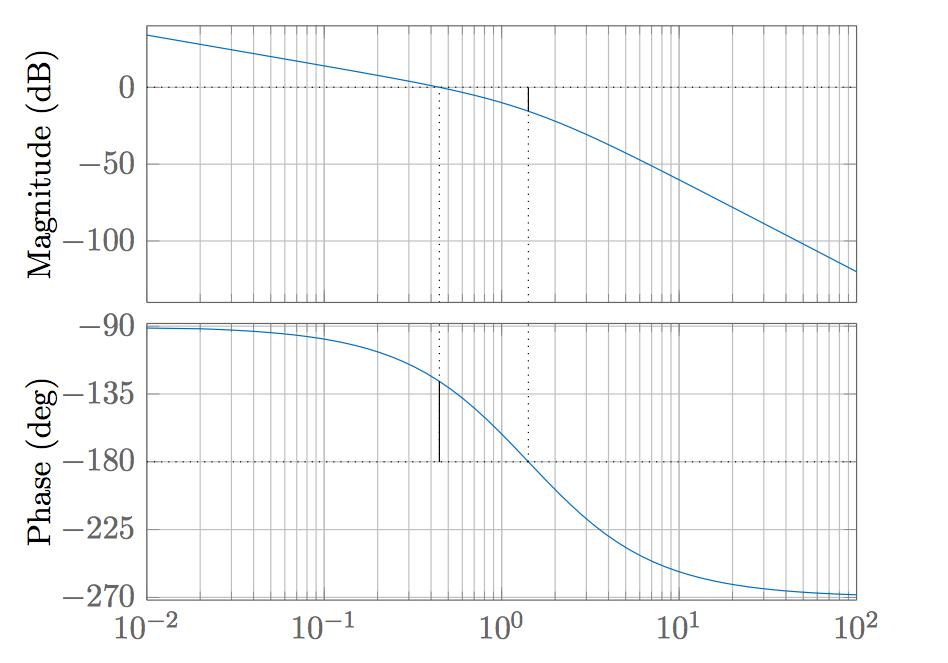
\includegraphics[width=0.7\columnwidth]{margins1.png}
\caption{Bodeplot with phase and gain margin}
\label{fig:margins1}
\end{center}
\end{figure}
\begin{figure}[h!]
\begin{center}
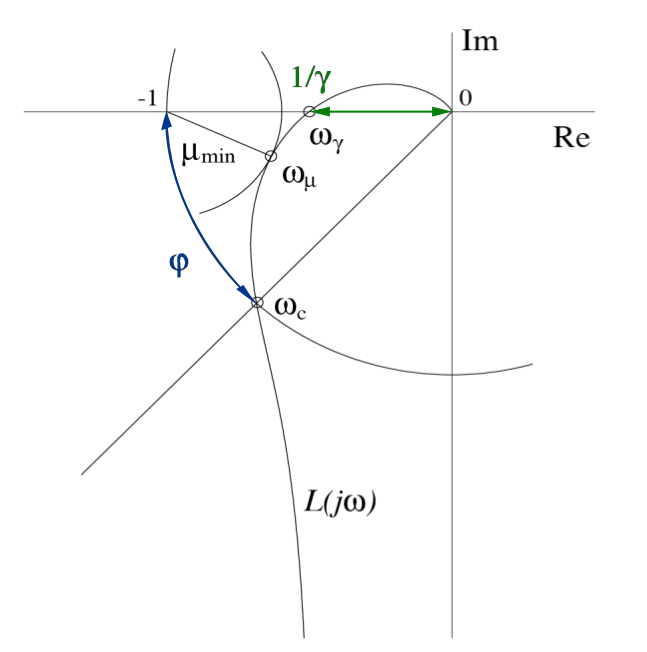
\includegraphics[width=0.65\columnwidth]{margins2.png}
\caption{Nyquist plot with phase and gain margin}
\label{fig:margins2}
\end{center}
\end{figure}

\newpage
 \subsection{Nyquist theorem}
A closed-loop system $T(s)$ is asymptotically stable if
\begin{equation}
n_c=n_+ +\frac{n_0}{2}.
\end{equation}
holds, where
\begin{itemize}
\item $n_c$: Number of mathematical positive encirclements of $L(s)$ about critical point $-1$ (counterclockwise).
\item $n_+$: Number of unstable poles of $L(s)$ ($Re(\pi)>0$).
\item $n_0$: Number marginal stable poles of $L(s)$ ($Re(\pi)=0$).

\end{itemize}

\subsection{Specifications for the closed-loop}
The main objective of control systems is to design a controller. Before one does this, one should be sure that the system is controllable. We learned that the controllability and observability are powerful tools to do that, but they are not enough: there are some others conditions for the \textbf{crossover-frequency} $\omega_c$ that should be fulfilled for the system in order to design a controller. It holds
\begin{equation}
\max(10\cdot \omega_d,2\cdot \omega_{\pi^+})<\omega_c<\min(0.5\cdot \omega_{\zeta^+},0.1\cdot \omega_n,0.5\cdot \omega_{\text{delay}},0.2\cdot \omega_2),
\end{equation}
where
\begin{itemize}
\item \makebox[2.5cm][l]{$\omega_{\pi^+}=\text{Re}({\pi^+})$:} Dominant (biggest with $\text{Re}(\pi)>0$) unstable Pole;
\item\makebox[2.5cm][l]{$\omega_{\zeta^+}=\text{Re}({\zeta^+})$:} Dominant (smallest with $\text{Re}(\zeta)>0$) nonminimumphase zero;
\item\makebox[2.5cm][l]{$\omega_d$:} Biggest disturbance-frequency of the system;
\item\makebox[2.5cm][l]{$\omega_n$:} Smallest noise-frequency of the system;
\item\makebox[2.5cm][l]{$\omega_2$:} Frequency with 100\% uncertainty ($|W_2(j\cdot \omega_2)|=1$),
\item\makebox[2.5cm][l]{$\omega_\text{delay}=\frac{1}{T_\text{delay}}$:} Biggest delay of the System.
\end{itemize}
\newpage
\subsection{Examples}
\begin{bsp}
The dynamic equations of a system are given as
\begin{equation*}
\begin{align}
\dot{x}_1(t)&=x_1(t)-5x_2(t)+u(t),\\
\dot{x}_2(t)&=-2x_1(t),\\
\dot{x}_3(t)&=-x_2(t)-2x_3(t),\\
y(t)&=3x_3(t).
\end{align}
\end{equation*}

\begin{enumerate}[(a)]
\item Draw the \textbf{Signal Diagram} of the system.
\item Find the \textbf{state space description} of the above system and write it in \textsc{Matlab}.
\item Find out if the system is \textbf{Lyapunov} stable or not, in \textsc{Matlab}.
\item Find the \textbf{Controllability} matrix and determine if the system is controllable in, \textsc{Matlab}.
\item Find the \textbf{Observability} matrix and determine if the system is observable, in \textsc{Matlab}.
\item Find the \textbf{transfer function} of the system with its poles and zeros, in \textsc{Matlab} 

\end{enumerate}
\newpage
\begin{lsg}
\
\begin{enumerate}[(a)]
\item The \textbf{Signal Diagram} reads

\end{enumerate}

\begin{figure}[h!]
\begin{center}
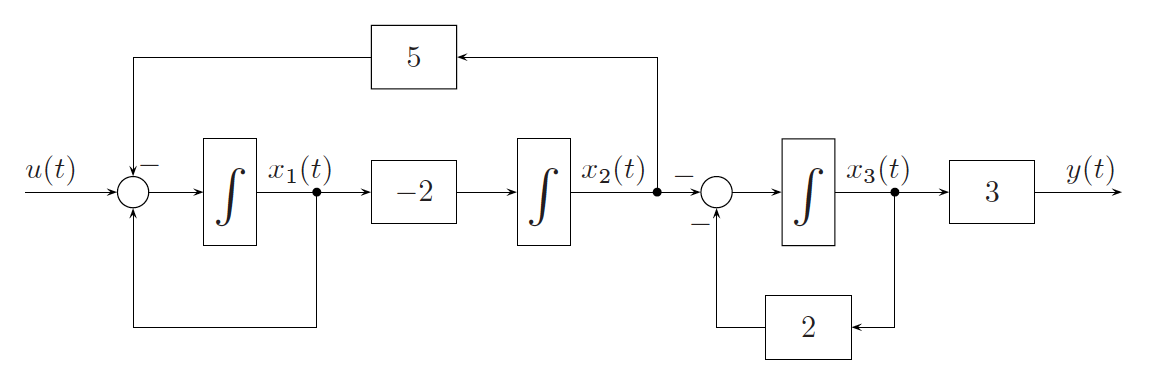
\includegraphics[width=0.85\columnwidth]{signal.png}
\caption{Signal Diagram of \textbf{Example 1.} }
\label{fig:signal}
\end{center}
\end{figure}

\begin{enumerate}[(b)]
\item The state space description has the following matrices:
\end{enumerate}
\begin{equation*}
A=\begin{pmatrix}
1&-5&0\\
-2&0&0\\
0&-1&-2\\
\end{pmatrix}, \qquad b=\begin{pmatrix}
1\\
0\\
0\\
\end{pmatrix}, \qquad c=\begin{pmatrix}
0&0&3
\end{pmatrix},\qquad d=0.
\end{equation*}
For the rest of solution \textbf{(b)} and solutions \textbf{(c)-(f)} see the attached \textsc{Matlab} script: \verb+Example_1_EC1.m+.
\end{lsg}
\end{bsp}
\newpage
\begin{bsp}
Given are a plant $P(s)=\frac{1}{(s+1)\cdot (s+2)}$ and its controller $C(s)=\frac{4}{(s+1)}$.
\begin{enumerate}[(a)]
\item Compute $L(s)$ and $T(s)$, with \textsc{Matlab}.
\item Find the \textbf{gain} and the \textbf{phase} margin numerically and plot them, with \textsc{Matlab}.
\item Write the \textbf{Bodeplot} of $P(s),C(s),L(s)$, \textsc{Matlab}.
\item Write the \textbf{Nyquist} plot of $P(s),L(s)$, with \textsc{Matlab}.
\item Plot the \textbf{Step response} for the open and closed loop, with \textsc{Matlab}
\item Plot the \textbf{Impulse response} for the open and the closed loop, with \textsc{Matlab}

\end{enumerate}

\begin{lsg}
See the attached \textsc{Matlab} script: \verb+Example_2_EC1.m+.

\end{lsg}


\end{bsp}
\newpage


\section{Synthesis of SISO Control Systems}
\subsection{Loop Shaping}
\subsubsection{Plant inversion}
This method isn't indicated for nonminimumphase plants and for unstable plants: in those cases this would lead to nonminimumphase or unstable controllers. This method is indicated for \textit{simple} systems for which it holds
\begin{itemize}
\item Plant is asymptotically stable.
\item Plant is minimumphase.
\end{itemize}
The method is then based on a simple step:
\begin{equation}
L(s)=C(s)\cdot P(s) \Rightarrow C(s)=L(s)\cdot P(s)^{-1}.
\end{equation}
The choice of the loop gain is free: it can be chosen such that it meets the specifications. 

\subsubsection{Loop shaping for Nonminimumphase systems}
A nonminimumphase system shows a wrong response: a change in the input results in a change in sign, that is, the system initially lies. Our controller should therefore be \textit{patient} and for this reason we use a \textit{slow} control system. This is obtained by a crossover frequency that is smaller than the nonminimumphase zero.
One begins to design the controller with a \textbf{PI-Controller}.
\begin{equation}
C(s)=k_p\cdot \frac{T_i\cdot s+1}{T_i\cdot s}.
\end{equation}
where parameters $k_p$ and $T_i$ can be chosen such that the loop gain $L(s)$ meets the known specifications. One can reach better robustness with \textbf{Lead/Lag} elements of the form
\begin{equation}
C(s)=\frac{T\cdot s+1}{\alpha \cdot T\cdot s+1}.
\end{equation}
where $\alpha,T \in \mathbb{R}^+.$ One can understand the Lead and the Lag as
\begin{itemize}
\item $\alpha<1$: \textbf{Lead-Element}: 
\begin{arrowlist}
 \item Phase margin increases.
 \item Loop gain increases.
\end{arrowlist}
\item $\alpha>1$: \textbf{Lag-Element}: 
\begin{arrowlist}
 \item Phase margin decreases.
 \item Loop gain decreases.
\end{arrowlist}
\end{itemize}
Like one can see in Figure \ref{fig:lead} and Figure \ref{fig:lag} the maximal benefits are reached at frequencies ($\hat{\omega}$) where the drawbacks are not yet fully developed.

\begin{figure}[h!]
\begin{center}
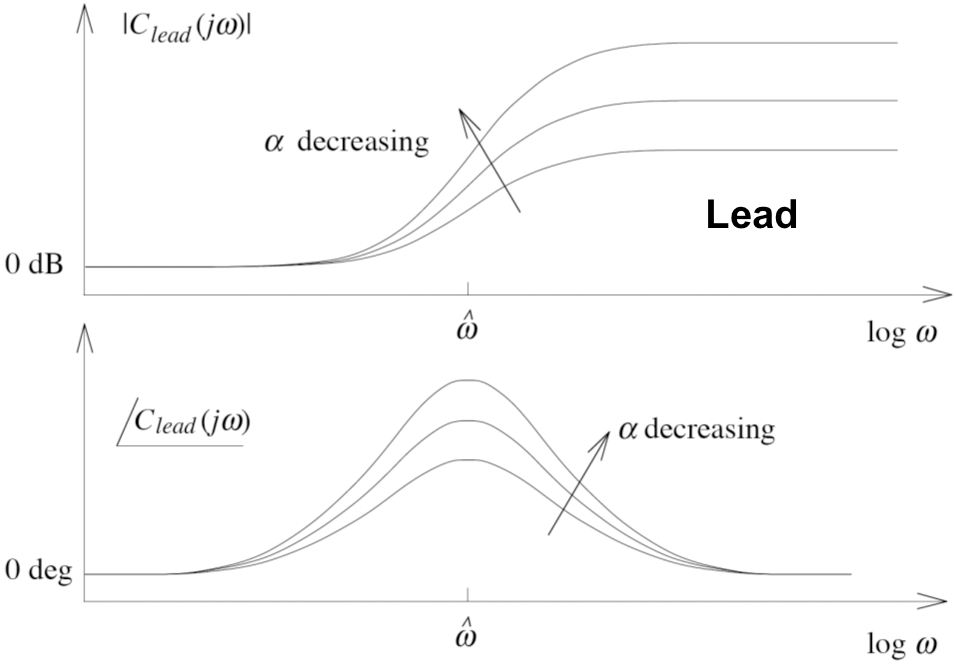
\includegraphics[width=0.65\columnwidth]{lead.png}
\caption{Bodeplot of lead Element}
\label{fig:lead}
\end{center}
\end{figure}

\begin{figure}[h!]
\begin{center}
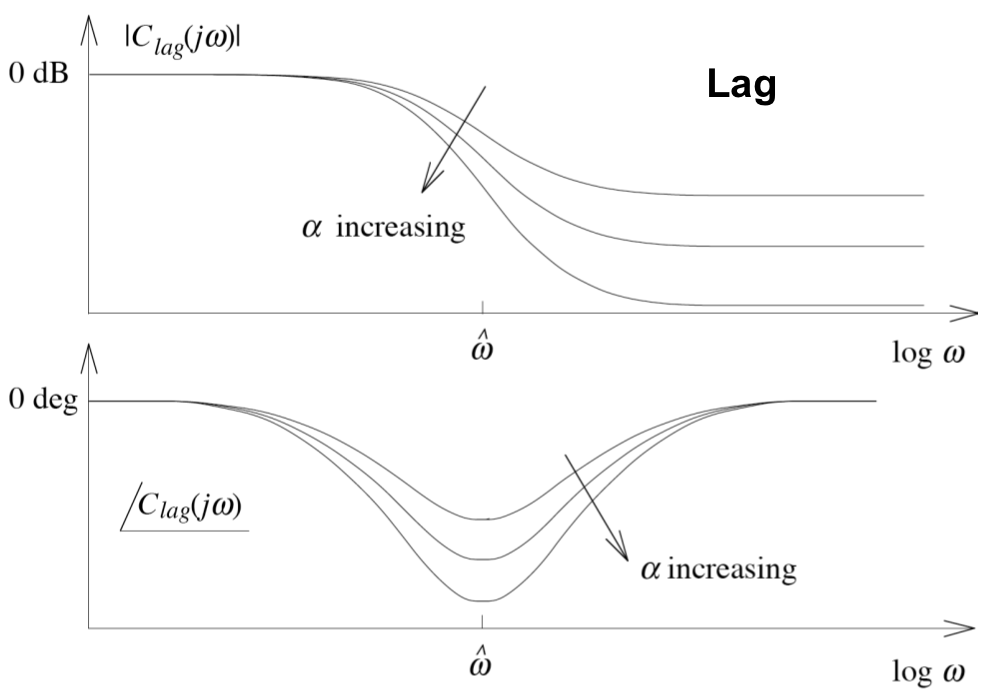
\includegraphics[width=0.65\columnwidth]{lag.png}
\caption{Bodeplot of lag Element}
\label{fig:lag}
\end{center}
\end{figure}
 
The element's parameters can be calculated as
\begin{equation}
\alpha=\left( \sqrt{\tan^2(\hat{\varphi})+1} -\tan(\varphi)\right)^2=\frac{1-\sin(\hat{\varphi})}{1+\sin(\hat{\varphi})}
\end{equation}
and
\begin{equation}
T=\frac{1}{\hat{\omega}\cdot \sqrt{\alpha}}.
\end{equation}
where $\hat{\omega}$ is the desired \textbf{center frequency} and $\hat{\varphi}=\varphi_{new}-\varphi$ is the desired \textbf{maximum phase shift} (in $rad$).
The classic loop-shaping method reads:
\begin{enumerate}
\item Design of a PI(D) controller.
\item Add Lead/Lag elements where needed\footnote{$L(j\omega)$ often suits not the learned requirements}
\item Set the gain of the controller $k_p$ such that we reach the desired crossover frequency.
\end{enumerate}
\newpage
\subsubsection{Loop shaping for unstable systems}
Since the Nyquist's theorem should always hold, if it isn't the case, one has to design the controller such that $n_c=n_+ +\frac{n_0}{2}$ is valid. To remember is: stable poles \textit{decrease} the phase by 90$\degree$ and minimumphase zeros \textit{increase} the phase by $ 90\degree$
\subsubsection{Feasibility}
Once the controller is designed, one has to look if this is really feasible and possible to implement. That is, if the number of poles is equal or bigger than the number of zeros of the system. If that is not the case, one has to add poles at high frequencies, such that they don't affect the system near the crossover frequency. One could e.g. add to a PID controller a \textit{Roll-Off Term} as
\begin{equation}
C(s)=\underbrace{k_p\cdot \left(1+\frac{1}{T_i \cdot s}+T_d\cdot s \right)}_{\text{PID Controller}}\cdot \underbrace{\frac{1}{(\tau \cdot s+1)^2}}_{\text{Roll-Off Term}}.
\end{equation}


\newpage

\subsection{Cascaded Control Systems}


Single input single output (SISO) systems use, in feedback control, the output $y$ as unique information to compute $u$. Clearly this doesn't represent a big part of the systems existing in the real world. \\
A first step towards a more precise solution, is to consider a situation where multiple outputs are available: the single input multiple output case (SIMO). To analyze such systems we need the theory and the methods that will be learned for the multiple input multiple output (MIMO) case. One can but still, without introducing this theory, use the concepts learned so far to handle such a system.

\subsubsection{Structure of cascaded systems}
The structure of a cascaded system can be seen in Figure \ref{fig:casc1}. Special cases that you could encounter in exercises can be seen in Figure \ref{fig:casc2} and Figure \ref{fig:casc3}. .
\begin{figure}[h]
\begin{center}
\begin{tikzpicture}[auto,node distance=2.5cm]%[auto, node distance=2cm,>=latex']
    \node [input, name=input] {};
    \node [sum, right of=input] (sum) {};
    \node [block, right = 1 cm of sum] (controller) {$C_\text{s}(s)$};
    \node [sum, right = 1cm of controller] (sum1) {};
    \node [block, right = 1cm of sum1] (controller1) {$C_\text{f}(s)$};
    \node [block, right of=controller1] (system) {$P_\text{f}(s)$};
    \node [block, right of=system] (system1) {$P_\text{s}(s)$};
    \node [output, right of=system1] (output) {};

    \draw [->] (input) -- node {$r_\text{s}$} (sum); % connections
    \draw [->] (sum) -- node {$e_\text{s}$} (controller);
    \draw [->] (controller) -- node {$r_\text{f}$} (sum1);
    \draw [->] (sum1) -- node {$e_\text{f}$} (controller1);
    \draw [->] (controller1) -- node {$u_\text{f}$} (system);
    \draw [->] ([yshift=5pt]system.east) -- node[name=us] {$u_\text{s}$} ([yshift=5pt]system1.west);
    
    \node [input, below = 1.5cm of us] (input1) {};
    
    \draw [-] ([yshift=-5pt]system) -| node[right,pos=0.80] {$y_\text{f}$} (input1);
    \draw [->] (input1) -| node[right,pos=0.97] {$-$} (sum1);
    
    \draw [->] (system1) -- node[name=ys] {$y_\text{s}$} (output);
    
    \node [input, below = 2cm of ys] (input2) {};
    
    \draw [-] (ys) -- node[name=ys] {} (input2);
    \draw [->] (input2) -| node[right,pos=0.98] {$-$} (sum);
    

\end{tikzpicture}
\caption{Control loop structure of a cascaded system.}
\label{fig:casc1}
\end{center}
\end{figure}


\begin{figure}[h]
\begin{center}
\begin{tikzpicture}[auto,node distance=2.5cm]%[auto, node distance=2cm,>=latex']
    \node [input, name=input] {};
    \node [sum, right of=input] (sum) {};
    \node [block, right = 1 cm of sum] (controller) {$C_\text{s}(s)$};
    \node [sum, right = 1cm of controller] (sum1) {};
    \node [block, right = 1cm of sum1] (controller1) {$C_\text{f}(s)$};
    \node [block, right of=controller1] (system) {$P_\text{f}(s)$};
    \node [block, right of=system] (system1) {$P_\text{s}(s)$};
    \node [output, right of=system1] (output) {};

    \draw [->] (input) -- node {$r_\text{s}$} (sum); % connections
    \draw [->] (sum) -- node {$e_\text{s}$} (controller);
    \draw [->] (controller) -- node {$r_\text{f}$} (sum1);
    \draw [->] (sum1) -- node {$e_\text{f}$} (controller1);
    \draw [->] (controller1) -- node {$u_\text{f}$} (system);
    \draw [->] (system.east) -- node[name=us] {} (system1.west);
    
    \node [input, below = 1.5cm of us] (input1) {};
    
    \draw [-] (system) -| node[right,pos=0.80] {$y_\text{f}$} (input1);
    \draw [->] (input1) -| node[right,pos=0.97] {$-$} (sum1);
    
    \draw [->] (system1) -- node[name=ys] {$y_\text{s}$} (output);
    
    \node [input, below = 2cm of ys] (input2) {};
    
    \draw [-] (ys) -- node[name=ys] {} (input2);
    \draw [->] (input2) -| node[right,pos=0.98] {$-$} (sum);
\end{tikzpicture}
\caption{Control loop structure of a cascaded system (with $u_\text{s}=y_\text{f}$).}
\label{fig:casc2}
\end{center}
\end{figure}


The main idea here is to divide the system basing on its \textit{time-scale}. Usually, one sets an inner \textit{faster} loop and an outer \textit{slower} loop. One can identify these elements in the fast dynamic's plant $P_f(s)$ and in the slow dynamic's plant $P_s(s)$. Basically, one wants to design a \textit{faster controller} $C_f(s)$ for the inner loop and a \textit{slower controller} $C_s(s)$ for the outer loop. 


\subsubsection{Time-Scale Estimation}
How can we distinguish between a \textit{slower} and a \textit{faster} control loop? A good way to do it consists in looking at the poles and the delays of the plant.
Let's have a look at the Inverse Laplace Transfrom of the output function $Y(s)$:
\begin{equation}\label{inverse3}
y(t)=\sum_{i=1}^p\sum_{k=1}^{\phi_i}\frac{\rho_{i,k}}{(k-1)!}\cdot t^{k-1}\cdot e^{\pi_i\cdot t}\cdot h(t).
\end{equation}
The dynamics of the plant are described by the absolutely \textit{smallest} pole. 

\begin{bsp}
We are given two plants $P_1(s)$ und $P_2(s)$. The poles $\pi_1$ und $\pi_2$ can be seen in the following table. We have to distinguish between $P_s(s)$ and $P_f(s)$. \\ \\
\begin{minipage}{.5\columnwidth}
\begin{center}
1)\qquad \begin{tabular}{ccc}\toprule
System & $\pi_1$ & $\pi_2$ \\ \midrule
$P_1(s)$ & $-1$ & $-100$ \\
$P_2(s)$ & $-10$ & $-50$ \\ \bottomrule
\end{tabular}
\end{center}
\end{minipage}
\begin{minipage}{.5\columnwidth}
\begin{center}
2)\qquad \begin{tabular}{ccc}\toprule
System & $\pi_1$ & $\pi_2$ \\ \midrule
$P_1(s)$ & $-1$ & $100$ \\
$P_2(s)$ & $-1$ & $10$ \\ \bottomrule
\end{tabular}
\end{center}
\end{minipage}
\begin{enumerate}[1)]
\item $P_1(s)$ has the smallest pole: this means $P_s(s)=P_1(s)$ and $P_f(s)=P_2(s)$.
\item Both systems share the same smallest pole. This means that as there isn't a different time-scale, the two systems should not be controlled with the cascaded control principle.
\end{enumerate}
\end{bsp}

\subsubsection{Design Process}
\subsubsection*{Faster Loop}
The faster controller $C_f(s)$ is (e.g. with Ziegler and Nichols) designed first without taking into account the slower loop. In order to exploit the most of the available bandwidth\footnote{An Integrator reduces the bandwidth. The bandwidth defines where our controller is working: we want the controller to have an action/reaction as big as possible.}, one chooses a P(D) controller, without the integrator.
\subsubsection*{Slower Loop}
The slower controller $C_s(s)$ is (e.g. with Ziegler and Nichols) designed as second: here, one has to consider the faster closed loop as part of the \textit{new} plant. Since this controller should obtain accuracy, one usually include the integrator here and chooses a PI(D) controller\footnote{The integrator reduces the static error!}.

\newpage
\subsubsection{Examples}

\begin{bsp}
Figure \ref{fig:casc3} shows a single input multiple output (SIMO) loop, that should be controlled with cascaded control. The given transfer functions are
\begin{equation}
\begin{split}
P_f(s)&=\frac{1}{s+1},\\
P_s(s)&=\frac{1}{5s^2+6s+1}, \\
C_f(s)&=2.
\end{split}
\end{equation}

\begin{figure}[h]
\begin{center}
\begin{tikzpicture}[auto,node distance=2.5cm]%[auto, node distance=2cm,>=latex']
    \node [input, name=input] {};
    \node [sum, right of=input] (sum) {};
    \node [block, right = 1 cm of sum] (controller) {$C_\text{s}(s)$};
    \node [sum, right = 1cm of controller] (sum1) {};
    \node [block, right = 1cm of sum1] (controller1) {$C_\text{f}(s)$};
    \node [block, right of=controller1] (system) {$P_\text{s}(s)$};
    \node [block, below = 0.5cm of system] (system1) {$P_\text{f}(s)$};
    \node [output, right of=system] (output) {};
    \node [output, right = 0.5cm of system1] (output1) {};
    \node [output, below = 0.5cm of system1] (output2) {};

    \draw [->] (input) -- node {$r_\text{s}$} (sum); % connections
    \draw [->] (sum) -- node {$e_\text{s}$} (controller);
    \draw [->] (controller) -- node {$r_\text{f}$} (sum1);
    \draw [->] (sum1) -- node {$e_\text{f}$} (controller1);
    \draw [->] (controller1) -- node [name=uf] {$u_\text{f}$}  (system);
    \draw [->] (uf) |- node {} (system1);
    %\draw [->] (system.east) -- node[name=us] {} (system1.west);
    
    \node [input, below = 1.5cm of us] (input1) {};
    
    \draw [-] (system1.east) |- node[above,pos=0.9] {$y_\text{f}$} (output1);
    \draw [-] (output1) |- node[left] {} (output2);
    \draw [->] (output2) -| node[right,pos=0.97] {$-$} (sum1);
    
    \draw [->] (system) -- node[name=ys] {$y_\text{s}$} (output);
    
    \node [input, below = 3cm of ys] (input2) {};
    
    \draw [-] (ys) -- node[name=ys] {} (input2);
    \draw [->] (input2) -| node[right,pos=0.98] {$-$} (sum);
    

\end{tikzpicture}
\caption{Control loop structure of a cascaded system.}
\label{fig:casc3}
\end{center}
Compute the transfer function of $P_{out}(s):r_f\rightarrow y_s$.
\end{figure}



\newpage
\begin{lsg}
To solve such problems, one has to work step by step. First, we use the frequency domain to determine the signals' dependencies. It holds:
\begin{equation}
\begin{split}
Y_s(s)&=P_s(s)\cdot U_f(s),\\
\end{split}
\label{fig:prima}
\end{equation}

where
\begin{equation}
\begin{split}
U_f(s)&=C_f(s)\cdot \left( R_f(s)-P_f(s)\cdot U_f(s)\right)\\
U_f(s)\cdot \left( 1+P_f(s)\cdot C_f(s)\right)&=C_f(s)\cdot R_f(s)\\
U_f(s)&=\frac{C_f(s)\cdot R_f(s)}{1+P_f(s)\cdot C_f(s)}.
\end{split}
\label{fig:sec}
\end{equation}

\ref{fig:sec} in \ref{fig:prima} gives
\begin{equation}
\begin{split}
P_{out}(s)=\frac{Y_s(s)}{R_f(s)}&=P_s(s)\cdot \frac{C_f(s)}{1+P_f(s)\cdot C_f(s)}\\
&=\frac{1}{5s^2+6s+1} \cdot \frac{2\cdot (s+1)}{(s+3)}\\
&=\frac{2}{(5s+1)\cdot (s+3)}.
\end{split}
\end{equation}







\end{lsg}


\end{bsp}




\newpage

\begin{bsp}
\
Consider the heated water tank depicted in Figure \ref{fig:wt}. The goal of this exercise is to design a controller for this system. The \textbf{valve position} $u$ should be controlled such that the \textbf{outlet water temperature} $T_w$ follows a given reference $T_{w,ref}$. The water outlet temperature, as well as the \textbf{steam mass flow} $\dot{m}_S$, are measured. Cascaded control can be used and the chosen controller structure is depicted in Figure \ref{fig:wtblock}.

\begin{figure}[H]
\begin{center}
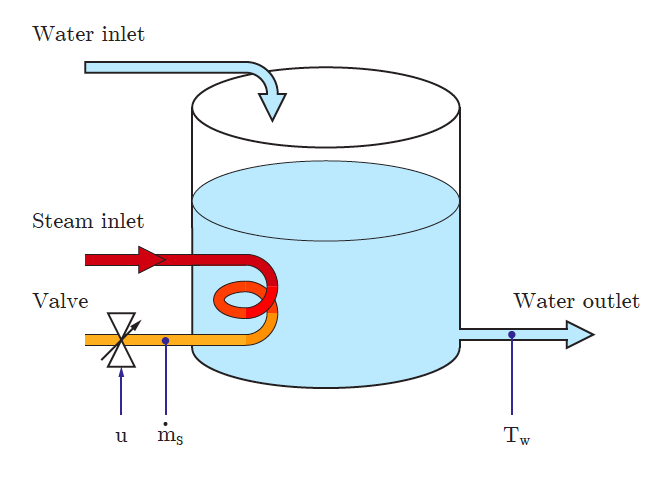
\includegraphics[width=0.75\columnwidth]{wt.png}
\caption{Heating water in the water tank.}
\label{fig:wt}
\end{center}
\end{figure}
\begin{figure}[h]
\begin{center}
\begin{tikzpicture}[auto,node distance=2.5cm]%[auto, node distance=2cm,>=latex']
    \node [input, name=input] {};
    \node [sum, right of=input] (sum) {};
    \node [block, right = 1 cm of sum] (controller) {$C_\text{s}(s)$};
    \node [sum, right = 1cm of controller] (sum1) {};
    \node [block, right = 1cm of sum1] (controller1) {$C_\text{f}(s)$};
    \node [block, right of=controller1] (system) {$P_\text{f}(s)$};
    \node [block, right of=system] (system1) {$P_\text{s}(s)$};
    \node [output, right of=system1] (output) {};

    \draw [->] (input) -- node {$r_\text{s}$} (sum); % connections
    \draw [->] (sum) -- node {$e_\text{s}$} (controller);
    \draw [->] (controller) -- node {$r_\text{f}$} (sum1);
    \draw [->] (sum1) -- node {$e_\text{f}$} (controller1);
    \draw [->] (controller1) -- node {$u_\text{f}$} (system);
    \draw [->] (system.east) -- node[name=us] {} (system1.west);
    
    \node [input, below = 1.5cm of us] (input1) {};
    
    \draw [-] (system) -| node[right,pos=0.80] {$y_\text{f}$} (input1);
    \draw [->] (input1) -| node[right,pos=0.97] {$-$} (sum1);
    
    \draw [->] (system1) -- node[name=ys] {$y_\text{s}$} (output);
    
    \node [input, below = 2cm of ys] (input2) {};
    
    \draw [-] (ys) -- node[name=ys] {} (input2);
    \draw [->] (input2) -| node[right,pos=0.98] {$-$} (sum);
\end{tikzpicture}
\caption{Control loop structure of the cascaded system.}
\label{fig:wtblock}
\end{center}
\end{figure}
\begin{enumerate}[(a)]
\item Which values of the system correspond to the signals $r_f,y_f,r_s$ and $y_s$?
\item Derive the outer/slow closed-loop transfer function $T_{r_s\rightarrow y_s}$ as a function of the closed-loop transfer function $T_{r_f\rightarrow y_f}$.
\end{enumerate}
\newpage
\begin{lsg}
\
\begin{enumerate}[(a)]
\item The two values that describe this system are the steam mass flow $\dot{m}_S$ and the water outlet temperature $T_w$. The temperature changes significantly slower than the steam mass flow, hence: the output of the outer/slower control loop $y_s$ corresponds to the water outlet temperature $T_w$. Its reference signal $r_s$ is the reference of this temperature $T_{w,ref}$. \\
The output of the inner/fast control loop $y_f$ corresponds to the steam mass flow $\dot{m}_S$. Its reference signal $r_f$ is the reference of the steam mass flow $\dot{m}_{S,ref}$.
\item The transfer function of the inner/fast closed-loop is
\begin{equation*}
\begin{split}
T_{r_f\rightarrow y_f}&=T_f\\
&=\frac{L_f}{1+L_f}\\
&=\frac{C_f\cdot P_f}{1+C_f\cdot P_f}.
\end{split}
\end{equation*}
The transfer function of the outer/slow closed-loop is
\begin{equation*}
\begin{split}
T_{r_f\rightarrow y_f}&=T_s\\
&=\frac{L_s}{1+L_s}\\
&=\frac{C_s\cdot T_f\cdot P_s}{1+C_s\cdot T_f\cdot P_s}.
\end{split}
\end{equation*}

\end{enumerate}

\end{lsg}


\end{bsp}
\newpage


\subsection{Predictive Control}
\subsubsection{Why predictive control}
If a system has \textit{substantial} delays, it is very difficult to control with a normal PID controller. The I part of the controller causes \textit{impatience}, that is, integrates overtime. As a practical example think of taking a shower at morning: one let the water flow and of course this hasn't the desired temperature. For this reason one chooses warmer water by turning the temperature controller, the water becomes too hot and so one turns it to colder water and so on, resulting in a non optimal strategy. Moreover, the D part of the controller is practically unuseful\footnote{Taking the derivative of a delay element doesn't help to control it}.
What does the expression \textit{substantial} delays mean? As indicative range one can say that it is worth using predictive control if
\begin{equation}
\frac{T}{T+\tau}>0.3,
\end{equation}
where $T$ is the delay and $\tau$ is the time constant of the system. Other prerequisites are
\begin{itemize}
\item The plant must be asymptotically stable.
\item A good model of the plant should be available.
\end{itemize}

\subsubsection{The Smith Predictor}
One can see the two \textit{equivalent} structures of the Smith Predictor in Figure \ref{fig:smith1} and Figure \ref{fig:smith2}.
\begin{figure}[h]
\begin{center}
\begin{tikzpicture}[auto,node distance=2.5cm]%[auto, node distance=2cm,>=latex']
    \node [input, name=input] {};
    \node [sum, right of=input] (sum) {};
    \node [block, right of=sum] (controller) {$C_\text{r}(s)$};
    \node [sum, right of=controller,pin={[pinstyle]above:$w$}] (sum1) {};
    \node [block, right of=sum1] (system) {$P_\text{r}(s)$};
    \node [block, right of=system] (totzeit) {$e^{-T\cdot s}$};
    \node [output, right of=totzeit] (output) {};
    \node [block, below =1 cm of totzeit] (totzeit1) {$e^{-\hat T\cdot s}$};
   
    \node [block, below = 1cm of system] (system1) {$\hat{P}_\text{r}(s)$};
    
    \draw [->] (controller) -- node[name=u] {$u$} (sum1); % connections
    \draw [->] (sum1) -- node[name=u1] {} (system);
    \draw [->] (system1) -- node [name=yr]{$\hat{y}_\text{r}$} (totzeit1);
    \draw [->] (totzeit) -- node [name=y] {$y$}(output);
    
    \node [sum, below = 1cm of yr] (sum2) {}; % extra node
    \node [sum, right = 0.73 cm of totzeit1] (sum3) {};
    
    \draw [->] (input) -- node {$r$} (sum);
    \draw [->] (sum) -- node {} (controller);
    \draw [->] (u) |- node {} (system1);
    \draw [->] (system) -- node {$y_\text{r}$} (totzeit);
    \draw [->] (yr) -- node {} (sum2);
    \draw [->] (y) -- node {} (sum3);
    \draw [->] (totzeit1) -- node[below,pos=0.90] {$-$}  (sum3); 
    \draw [->] (sum2) -| node[right,pos=0.98] {$-$} (sum); 
    \draw [->] (sum3) |- node[above,pos=0.55] {$\epsilon$} (sum2); 
\end{tikzpicture}
\caption{Structure of the Smith predictor.}
\label{fig:smith1}
\end{center}
\end{figure}

\begin{figure}[h]
\begin{center}
\begin{tikzpicture}[auto,node distance=2.5cm]%[auto, node distance=2cm,>=latex']
    \node [input, name=input] {};
    \node [sum, right of=input] (sum) {};
    \node [sum, right = 0.75cm of sum] (sum1) {};
    \node [block, right = 0.75 cm of sum1] (controller) {$C_\text{r}(s)$};
    \node [block, below = 1cm of controller] (system1) {$\hat P_\text{r}(s)$};
    \node [sum, right = 0.5cm of system1] (sum2) {};
    \node [input, right = 1cm of sum2] (input2) {};
    \node [block, below = 1cm of input2] (totzeit1) {$e^{-s\cdot \hat T}$};
    \node [block, right = 3.5cm of controller] (system) {$P_\text{r}(s)$};
    \node [block, right of=system] (totzeit) {$e^{-s\cdot T}$};
    \node [output, right of=totzeit] (output) {};
    \node [input, below of=system1] (input1) {};
    \node [input, right = 3 cm of controller] (x) {};
    
    \draw [->] (input) -- node {$r$} (sum);
    \draw [->] (sum) -- node {$e$} (sum1);
    \draw [->] (sum1) -- node {} (controller);
    \draw [->] (controller) -- node {$u$} (system);
    \draw [->] (system) -- node {} (totzeit);
    \draw [->] (totzeit) -- node[name=y] {$y$} (output);
    \draw [->] (x) |- node  {} (sum2);
    \draw [->] (sum2) -- node  {} (system1);
    \draw [->] (system1) -| node[right,pos=0.98] {$-$}  (sum1);
    \draw [-] (y) |- node {}  (input1);
    \draw [->] (input1) -| node[right,pos=0.99] {$-$}  (sum);
    \draw [->] (x) |- node {} (totzeit1);
    \draw [->] (totzeit1) -| node[right,pos=0.97] {$-$}  (sum2);
    
    
    
    
   
\end{tikzpicture}
\caption{Structure of the Smith predictor.}
\label{fig:smith2}
\end{center}
\end{figure}

If the system has big delays, one can assume that it is possible to write the delay element and the nondelayed plant as a product in the frequency domain: that's what is done in the upper right side of Figure \ref{fig:smith1}. This means that the transfer function $u\rightarrow y$ can be written as
\begin{equation}
P(s)=P_r(s)\cdot e^{-sT}.
\end{equation}
\subsubsection*{Main Idea:} As long as we have no disturbance $w$ ($w=0$) and our model is good enough (this means $P_r(s)=\hat{P}_r(s),\ T=\hat{T}$)\footnote{We use $\hat{\hdots}$ to identify the parameters of the model}, we can model a non delayed plant and get the non delayed output $\hat{y}_r(t)$ (one can see this on the lower right side of Figure \ref{fig:smith1}). The feedback signal results from the sum of $\hat{y}_r(t)$ and the correction signal $\epsilon$.
\subsubsection{Analysis}
The controller of the system is the transfer function $e\rightarrow u$ , which can be computed as
\begin{equation}
\begin{split}
U(s)&=C_r(s)\cdot (R(s)-\hat{P}_r(s)\cdot U(s)+\hat{P}_r(s)\cdot e^{-s\hat{T}}\cdot U(s) -Y(s))\\
&=C_r(s)\cdot \underbrace{(R(s)-Y(s))}_{E(s)} - C_r(s)\cdot \hat{P}_r(s)\cdot (1-e^{-s\hat{T}})\cdot U(s).\\
\end{split}
\end{equation}
If one solves for $U(s)$:
\begin{equation}
U(s)=\frac{C_r(s)}{1+C_r(s)\cdot \hat{P}_r(s)\cdot(1-e^{-s\cdot\hat{T}})}\cdot E(s)
\end{equation}
and so the transfer function of the controller reads
\begin{equation}
C(s)=\frac{C_r(s)}{1+C_r(s)\cdot\hat P_r(s).\cdot(1-e^{-s\cdot\hat T})}.
\end{equation}
This means that the loop gain is
\begin{equation}
L(s)=P(s)\cdot C(s)=\frac{C_r(s)\cdot P_r(s)\cdot e^{-s\cdot T}}{1+C_r(s)\cdot\hat P_r(s)\cdot(1-e^{-s\cdot\hat T})}.
\end{equation}
If one assumes as stated, that the model is good enough s.t. $P_r(s)=\hat{P}_r(s),\ T=\hat{T}$, one gets
\begin{equation}
\begin{split}
T(s)&=\frac{L(s)}{1+L(s)} \\
&=\frac{\frac{C_\text{r}(s)\cdot P_\text{r}(s)\cdot e^{-s\cdot T}}{1+C_\text{r}(s)\cdot P_\text{r}(s)\cdot(1-e^{-s\cdot T})}}{1+\frac{C_\text{r}(s)\cdot P_\text{r}(s)\cdot e^{-s\cdot T}}{1+C_\text{r}(s)\cdot P_\text{r}(s)\cdot(1-e^{-s\cdot T})}} \\
&=\frac{C_\text{r}(s)\cdot P_\text{r}(s)\cdot e^{-s\cdot T}}{1+C_\text{r}(s)\cdot P_\text{r}(s)\cdot(1-e^{-s\cdot T})+C_\text{r}(s)\cdot P_\text{r}(s)\cdot e^{-s\cdot T}} \\
&=\frac{C_\text{r}(s)\cdot P_\text{r}(s)}{1+C_\text{r}(s)\cdot P_\text{r}(s)}\cdot e^{-s\cdot T} \\
&=T_\mathrm{ref}(s)\cdot e^{-s\cdot T}.
\end{split}
\end{equation}
\newpage
\begin{bmk}
\
\begin{itemize}
\item This result is very important: we have shown that the delay cannot be completely eliminated and that every tranfer function (here $T(s)$ but also $S(s)$) will have the same delay as the plant $P(s)$.
\item Advantages of the prediction are:
\begin{itemize}
\item Very fast.
\item Same Robustness.
\end{itemize}
\item Disadvantages of the prediction are:
\begin{itemize}
\item Very difficult to implement.
\item Very difficult to analyze.
\item Problems if there are model errors.
\end{itemize}

\end{itemize}
\end{bmk}

\newpage
\subsubsection{Examples}

\begin{bsp}
We want to control the plant $P(s)=P_r(s)\cdot e^{-s\tau}$ with a Smith Predictor. The structure of the predictor can be seen in Figure \ref{fig:smith3}.
\begin{figure}[h!]
\begin{center}
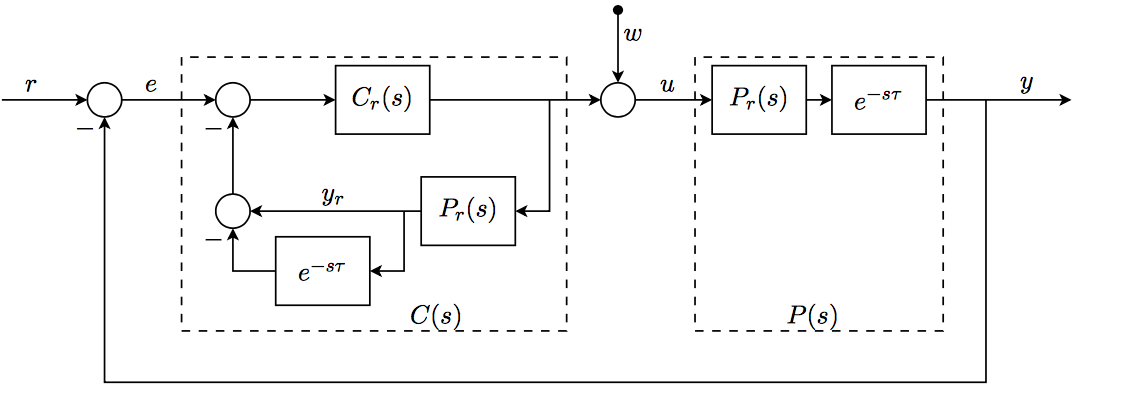
\includegraphics[width=0.86\columnwidth]{smith3.png}
\caption{Smith Predictor Structure}
\label{fig:smith3}
\end{center}
\end{figure}

\begin{enumerate}[(a)]
\item Assume that the model isn't that good and derive the transfer functions of
\begin{enumerate}[i)]
\item The controller.
\item The loop gain.
\item The complementary sensitivity.
\end{enumerate}

\end{enumerate}

\begin{enumerate}[(b)]
\item Let's say the model is now perfect. $T_r(s)$ should behave like a \textit{first order low-pass system} with cutoff frequency $a$. The gain should be chosen s.t. no static error is produced. Find such a $T_r(s)$. 
\end{enumerate}

\begin{enumerate}[(c)]
\item The plant has been modeled by a friend of you: he had no time for a complete job because of a hockey playoff match and he derived just the state space description of the system. This reads
\begin{equation*}
\dot{x}(t)=\begin{pmatrix}
0 & 1\\
0&0\\
\end{pmatrix} \cdot x(t)+\begin{pmatrix}
0\\
\frac{1}{m}
\end{pmatrix}\cdot u(t)
\end{equation*}
and
\begin{equation*}
\hat{y}(t)=\begin{pmatrix}
1&0
\end{pmatrix} \cdot x(t), \  y(t)=\hat{y}(t-\tau).
\end{equation*}

Find the transfer function of the plant.
\end{enumerate}

\begin{enumerate}[(d)]
\item Calculate the transfer function of the controller $C_r(s)$.
\end{enumerate}
\newpage
\begin{lsg} \
\begin{enumerate}[(a)]
\item \begin{enumerate}[i)]
\item Controller:\\
With the same derivation seen in the theory, one gets
\begin{equation*}
C(s)=\frac{C_r(s)}{1+C_r(s)\cdot\hat P_r(s)\cdot(1-e^{-s\cdot\hat{\tau}})}.
\end{equation*}
\item Loop Gain:\\
With the same derivation seen in the theory, one gets
\begin{equation*}
L(s)=\frac{C_r(s)\cdot P_r(s)\cdot e^{-s\cdot \tau}}{1+C_r(s)\cdot\hat P_r(s)\cdot(1-e^{-s\cdot\hat{\tau}})}.
\end{equation*}
\item Complementary Sensitivity:\\
With the same derivation seen in the theory, one gets
\begin{equation*}
\begin{split}
T(s)&=\frac{L(s)}{1+L(s)}\\
&=\frac{C_r(s)\cdot P_r(s)\cdot e^{-s\tau}}{1+C_r(s)\cdot \hat{P}_r(s)\cdot(1-e^{-s\hat{\tau}})+P_r(s)\cdot C_r(s)\cdot e^{-s\tau}}.
\end{split}
\end{equation*}


\end{enumerate}
\item With a perfect model, one gets
\begin{equation*}
\begin{split}
T(s)&=\frac{P_r(s)\cdot C_r(s)}{1+P_r(s)\cdot C_r(s)}\cdot e^{-s\tau}\\
&= T_r(s)\cdot e^{-s\tau}.
\end{split}
\end{equation*}
The general form for a lowpass system is
\begin{equation*}
\Sigma(s)=\frac{k}{\tau s+1}.
\end{equation*}
where $\omega=\frac{1}{\tau}$ the is cutoff frequency and $k$ is the gain. If we don't want a static error, the gain should be 1 ($k=1$).  This last step can be shown if one calculates the static error with the well-known formula. With the informations about the cutoff frequency one gets
\begin{equation*}
\begin{split}
T_r(s)&=\frac{1}{\frac{s}{a}+1}\\
&=\frac{a}{s+a}.
\end{split}
\end{equation*}

\item Here one should use Laplace Analysis. The two differential equations reads
\begin{equation*}
\begin{split}
\dot{x}_1(t)&=x_2(t), \\
\dot{x}_2(t)&=\frac{1}{m}\cdot u(t)
\end{split}
\end{equation*}
with
\begin{equation*}
\begin{split}
\hat{y}(t)&=x_1(t), \\
y(t)&=\hat{y}(t-\tau).
\end{split}
\end{equation*}
The Laplace transform leads to
\begin{equation*}
\begin{split}
sX_1(s)&=X_2(s)\\
sX_2(s)&=\frac{1}{m}\cdot U(s)
\end{split}
\end{equation*}
and
\begin{equation*}
\hat{Y}(s)=X_1(s), \ \ Y(s)=\hat{Y}(s)\cdot e^{-s\tau}
\end{equation*}
together:
$$s^2X_1(s)=\frac{1}{m}U(s)$$
and so
$$U(s)=ms^2X_1(s)$$
For the transfer function, it holds
\begin{equation*}
\begin{split}
P(s)&=\frac{Y(s)}{U(s)}\\
&=\frac{X_1(s)\cdot e^{-s\tau}}{X_1(s)\cdot ms^2}\\
&=\frac{1}{ms^2}\cdot e^{-s\tau}\\
&=P_r(s)\cdot e^{-s\tau}.
\end{split}

\end{equation*}

\item Since
\begin{equation*}
T_r(s)=\frac{P_r(s)\cdot C_r(s)}{1+P_r(s)\cdot C_r(s)}
\end{equation*}
by solving for $C_r(s)$ one gets
\begin{equation*}
\begin{split}
C_r(s)&=\frac{T_r(s)}{P_r(s)\cdot (1-T_r(s))}\\
&= \frac{\frac{a}{s+a}}{\frac{1}{ms^2}\cdot \left(1-\frac{a}{s+a}\right)}\\
&=\frac{ams^2}{s}\\
&=am\cdot s.
\end{split}
\end{equation*}





\end{enumerate}


\end{lsg}


\end{bsp}

\newpage
\subsection{Robustness}

\subsubsection{Robust Stability}
In order to determine the stability of the closed loop loop gain we have used the Nyquist theorem. That isn't enough: we have to consider that the model for $L(s)$ could be unprecise. In order to ensure stability, it should hold
\begin{equation}
|W_2(j\cdot \omega)\cdot L(j\cdot \omega)|<|1+L(j\cdot \omega)| \ \forall \omega \in [0,\infty].
\end{equation}
This condition can be reformulated, in order to use the complementary sensitivity $T(s)$:
\begin{equation}
\begin{split}
|W_2(j\cdot \omega)\cdot L(j\cdot \omega)|&<|1+L(j\cdot \omega)| \ \forall \omega \in [0,\infty]\\
\frac{|L(j\cdot \omega)|}{|1+L(j\cdot \omega)|}&<\frac{1}{|W_2(j\cdot \omega)|}\\
|T(j\cdot \omega)|&<\frac{1}{|W_2(j\cdot \omega)|}\\
|T(j\cdot \omega)|\cdot |W_2(j\cdot \omega)|&<1.
\end{split}
\end{equation}
This can be interpreted as an upper bound for the complementary sensitivity.

\subsubsection{Nominal Performance}
The conditions for the sensitivity $S(s)$ can be resumed in the transfer function $W_1(s)$ and so it must hold
\begin{equation}
\begin{split}
|W_1(j\cdot \omega)\cdot S(j\cdot \omega)|&<1\\
\frac{1}{|1+L(j\cdot \omega)|}\cdot |W_1(j\cdot \omega)|&<1\\
|W_1(j\cdot \omega)|&<|1+L(j\cdot \omega)|.
\end{split}
\end{equation}
which can be used in with the Nyquist plot: for each frequency $\omega$ the return difference should have a distance from the critical point -1 that is larger than $|W_1(j\cdot \omega)|$. Such a system is referred to as satisfying the \textit{nominal performance condition}.

\subsubsection{Robust Performance}
If a controller $C(s)$ also satisfies
\begin{equation}
|W_1(j\cdot \omega) \cdot S(j\cdot \omega)|+|W_2(j\cdot \omega) \cdot T(j\cdot \omega)|<1.
\end{equation}
then it satisfies the \textit{robust performance condition}, where, as reminder
\begin{itemize}
\item $|W_1(j\cdot \omega)|$: Bound for the sensitivity, from specifications.
\item $|W_2(j\cdot \omega)|$: Bound for the complementary sensitivity, from specifications.
\end{itemize}


Multiplying both sides by $|1+L(j\cdot \omega)|$ one gets the rearranged condition
\begin{equation}
|W_1(j\cdot \omega)| +|W_2(j\cdot \omega) \cdot L(j\cdot \omega)|<|1+L(j\cdot \omega)|.
\end{equation}

\begin{bmk}
The nominal and the robust perfomance conditions don't guarantee the stability of the system: this should be determined separately, e.g. with the Nyquist theorem.
These conditions can be easily checked with Figure \ref{fig:rob}
\end{bmk}
\begin{figure}[H]
\begin{center}
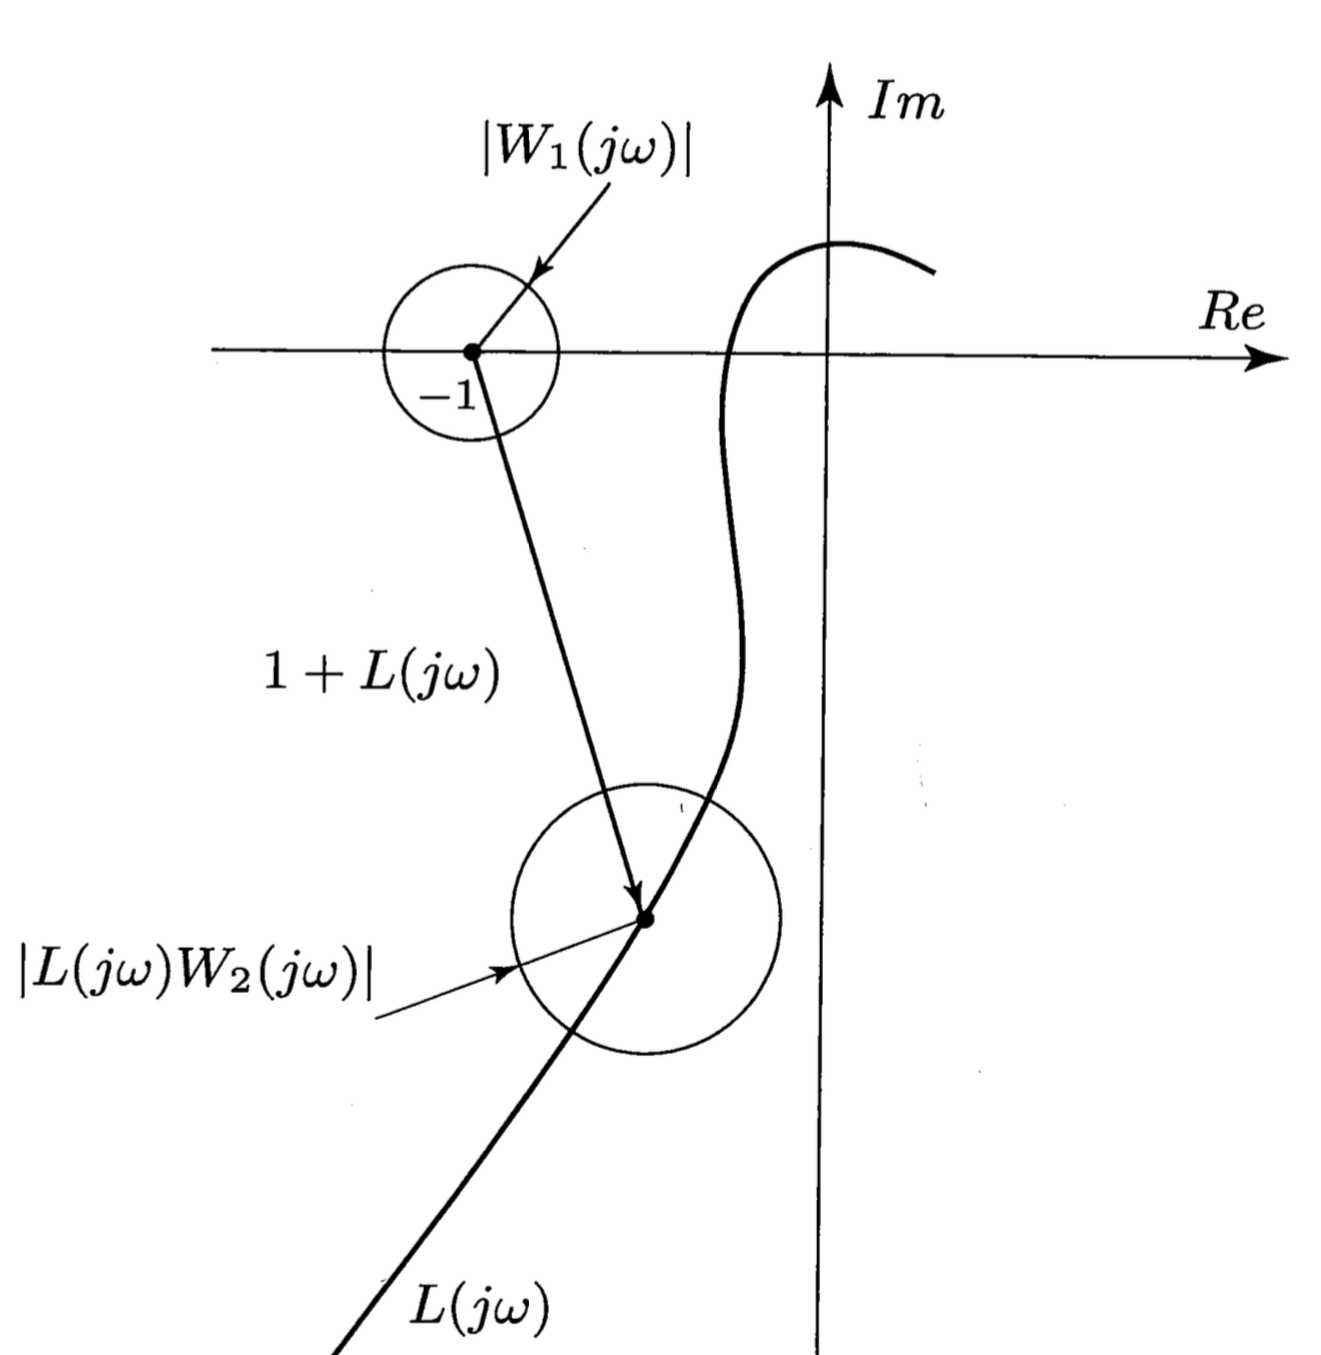
\includegraphics[width=0.7\columnwidth]{robust2.png}
\caption{Nyquist with conditions}
\label{fig:rob}
\end{center}
\end{figure}

\pagebreak

\subsubsection{Examples}
\begin{bsp}
In order to design a controller for the plant $P(s)$, a bound for the sensitivity of the control system is set:
\begin{equation*}
W_1(s)=60\cdot \frac{2\cdot s +1}{200\cdot s+1}.
\end{equation*}
Iteratively, one finds a good controller that results in the complementary sensitivity
\begin{equation*}
T(s)=\frac{\omega_0^2}{s^2+2\cdot \delta \cdot \omega_0 \cdot s+\omega_0^2}.
\end{equation*}
where $\omega_0=1\frac{\text{rad}}{\text{s}}$ and $\delta=1$.

\begin{enumerate}[(a)]
\item One can show that the maximal value of the sensitivity $|S(j\omega^*)|$ occurs at $\omega^*=\sqrt{2}$. Compute the value of $|S(j\omega^*)|$.
\item Show that the condition for nominal performance is fulfilled in $\omega^*$.
\item What is the limit value of $|W_2(j\omega^*)|$ in order to fulfill the condition for robust performance?\\
\textbf{Hint:} It holds $|L(j\omega^*)|=0.29$.
\end{enumerate}
\newpage
\begin{lsg}\
\begin{enumerate}[(a)]
\item 
\end{enumerate}
It holds
\begin{equation*}
\begin{split}
S(s)&=1-T(s)\\
&=1-\frac{1}{s^2+2\cdot s+1}\\
&=\frac{s^2+2\cdot s}{s^2+2\cdot s+1}.\\
S(j\omega)&=\frac{-\omega^2+2j\omega}{-\omega^2+2j\omega +1}\\
&=\frac{(-\omega^2+2j\omega)\cdot (1-\omega^2-2j\omega)}{(-\omega^2+2j\omega+1)\cdot (1-\omega^2-2j\omega)}\\
&=\frac{\omega^4+3\omega^2+2j\omega}{(1-\omega^2)^2+4\omega^2}.\\
|S(j\omega^*)|&=\left| \frac{10+j2\sqrt{2}}{9} \right|\\
&=\sqrt{\frac{108}{81}}=1.16.
\end{split}

\end{equation*}

\begin{enumerate}[(b)]
\item 
\end{enumerate}
The condition reads
\begin{equation*}
\begin{split}
|S(j\omega^*)|\cdot |W_1(j\omega^*)|&<1\\
\Rightarrow|S(j\omega^*)|&< \frac{1}{|W_1(j\omega^*)|}.
\end{split}

\end{equation*}
It holds
\begin{equation*}
\begin{split}
|W_1(j\omega^*)|&=\left| 60\cdot \frac{2j\omega^*+1}{200j\omega^*+1} \right|\\
&=60\cdot \left| \frac{(2j\omega^*+1)\cdot (1-200j\omega^*)}{(200j\omega^*+1)\cdot (1-200j\omega^*)} \right|\\
&=60\cdot \left| \frac{(1+400{\omega^*}^2-198j\omega^*)}{1+(200\cdot \omega^*)^2}\right|\\
&=60\cdot \frac{\sqrt{(1+400{\omega^*}^2)^2+(198\omega^*)^2}}{1+(200\cdot \omega^*)^2}\\
&=0.64.
\end{split}
\end{equation*}
Since
$$1.16<\frac{1}{0.64}=1.56$$
the condition is fulfilled for $\omega^*$.
\begin{enumerate}[(c)]
\newpage
\item 
\end{enumerate}
The condition reads
\begin{equation*}
\begin{split}
|W_1(j\cdot \omega^*)| +|W_2(j\cdot \omega^*) \cdot L(j\cdot \omega^*)|&<|1+L(j\cdot \omega^*)|\\
|W_1(j\cdot \omega^*)| +|W_2(j\cdot \omega^*) \cdot L(j\cdot \omega^*)|&<\left| \frac{1}{S(j\omega^*)} \right| \\
|W_2(j\cdot \omega^*)|&< \frac{1}{|L(j\cdot \omega^*)|}\cdot \left( \left| \frac{1}{S(j\omega^*)}\right|-|W_1(j\cdot \omega^*)|\right)\\
|W_2(j\cdot \omega^*)|&<\frac{1}{0.29}\cdot \left( \frac{1}{1.16}-0.64 \right)\\
|W_2(j\cdot \omega^*)|&<0.77.
\end{split}
\end{equation*}



\end{lsg}


\end{bsp}
\newpage
\section{Implementation of Controllers}
\subsection{Setpoint Weighting for PID}
\subsubsection{Recap Goals}


\begin{figure}[htbp]

\begin{center}
\begin{tikzpicture}[auto,node distance=2.5cm]%[auto, node distance=2cm,>=latex']
    \node [input, name=input] {};
    \node [sum, right of=input] (sum) {};
    \node [block, right of=sum] (controller) {$C(s)$};
    \node [sum, right of=controller,pin={[pinstyle]above:$w$}] (sum1) {};
    \node [block, right of=sum1] (system) {$P(s)$};
    \node [sum, right of=system,pin={[pinstyle]above:$d$}] (sum2) {};
    \node [output, right of=sum2] (output) {};
    
    \draw [->] (input) -- node {$r$} (sum);
    \draw [->] (sum) -- node {$e$} (controller);
    \draw [->] (controller) -- node[] {} (sum1);
    \draw [->] (sum1) -- node[] {$u$} (system);
    \draw [->] (system) -- node[] {} (sum2);
    \draw [->] (sum2) -- node[name=y] {$y$} (output);
    
    \node [sum, below of=y,pin={[pinstyle]right:$n$}] (sum3) {};
    
    \draw [->] (y) -- node[] {} (sum3);
    \draw [->] (sum3) -| node[right,pos=0.98] {$-$} (sum);
\end{tikzpicture}
\caption{Standard feedback control system's structure}
\end{center}

%\caption{Schema eines Systems mit R\"uckf\"uhrung}
The two big different goals for a control system are \textbf{reference tracking} and \textbf{disturbance rejection}. \\
\textbf{Reference Tracking:} Let $y(t)$ \textit{track} $r(t)$. \\
\textbf{Disturbance Rejection:} Keep $y(t)$ at $r(t)$. \\
\end{figure}
\subsubsection{Method}
Since these two goals are often not achievable with a single controller, we define a method to adapt easily the PID controller to different needs, by introducing the \textbf{weights} $a,b,c$.
\begin{figure}[h]
\begin{center}\includegraphics[width=5cm,angle=-90]{hagglund}\end{center}
\caption{Setpoint weighting PID structure.}
\end{figure}

By \textit{tuning} the weights $a,b,c$ one can achieve the desired control action. \\
One can write, mathematically:
\begin{equation}
U(s)=k_p\cdot(a\cdot R(s)-Y(s))+\frac{k_p}{T_i\cdot s}\cdot(b\cdot R(s)-Y(s))+k_p\cdot T_d\cdot s\cdot(c\cdot R(s)-Y(s)).
\end{equation}
\begin{bmk}
From this equation, one can show that the choice of $a,b,c$ has no influence on the loop gain, that is, no influence on the stability of the system.
\end{bmk}
\subsubsection{Application to Reference Tracking}
Although the PID controller was designed by thinking of some disturbance rejection problem, this method could also be used to ensure reference tracking. If \textbf{disturbances} are small compared to \textbf{reference changes} and the actuator is a \textbf{limiting factor} (see saturation, next chapters), usually one does the following choice:
\begin{itemize}
\item \textbf{P}: The parameter a is chosen such that: $0<a<1$.
\begin{itemize}
\item We can control the \textit{aggressivity} of the controller.
\end{itemize}
\item \textbf{I}: The parameter b is chosen such that: $b=1$.
\begin{itemize}
\item  with $r=y$ one has that $e_\infty \rightarrow 0$.
\end{itemize}
\item \textbf{D}: The parameter c is chosen such that: $c=0$.
\begin{itemize}
\item If there are disturbances, it is good not to have their influences on derivative terms.
\end{itemize}
\end{itemize}
\newpage
\subsubsection{Examples}
\begin{bsp}
A plant $P(s)$ should be controlled with a PID controller. One should consider the setpoint weighting in order to better design the controller. The plant reads
\begin{equation*}
P(s)=\frac{10}{(s+1)(s+2)(s+3)}.
\end{equation*}
\begin{enumerate}[(a)]
\item Find 
\begin{enumerate}[i)]
\item The critical time constant $T^*$,
\item The critical gain $k_p^*$,
\item The static gain of the plant.
\end{enumerate}
\item Derive the transfer function between $r\rightarrow y$. 
\end{enumerate}
\newpage
\begin{lsg} 
\
\begin{enumerate}[(a)]
\item
\end{enumerate}

With the rules learned in Control Systems I, it holds:
\begin{equation*}
\begin{split}
k_p^*\cdot P(j\omega^*) &= -1 + 0\cdot j\\
T^*&=\frac{2\pi}{\omega^*}.
\end{split}
\end{equation*}

With the defined plant:

\begin{equation*}
\begin{split}
k_p^*\cdot P(j\omega^*)&=\frac{10\cdot k_p^*}{(j\omega^*+1)\cdot(j\omega^*+2)\cdot(j\omega^*+3)}\\
&=\frac{10\cdot k_p^*}{-6\omega^{*^2}+6+j\cdot (-\omega^{*^3}+11\omega^*)}.
\end{split}
\end{equation*}
The imaginary part should be 0. It holds
\begin{equation*}
-\omega^{*^3}+11\omega^*=0 \Rightarrow \omega^*=\sqrt{11}.
\end{equation*}
The real part should be -1. It holds
\begin{equation*}
\frac{10\cdot k_p^*}{-6\omega^{*^2}+6}=-1 \Rightarrow k_p*=6.
\end{equation*}

The static gain is

\begin{equation*}
P(0)=\frac{10}{6}.
\end{equation*}

\begin{enumerate}[(b)]
\item
\end{enumerate}

It holds
\begin{equation*}
\begin{split}
Y(s)&=P(s)\cdot U(s)\\
&=P(s)\cdot \left( (aR(s)-Y(s))\cdot k_p + (bR(s)-Y(s))\cdot \frac{k_p}{T_i}\cdot \frac{1}{s}+(cR(s)-Y(s))\cdot k_p\cdot T_d\cdot s \right).
\end{split}
\end{equation*}
One can write
\begin{equation*}
R(s)\cdot P(s) \cdot k_p \cdot \left( a+\frac{b}{T_i \cdot s}+cT_d \right)=Y(s)\cdot \left(1+P(s)\cdot k_p\cdot (1+\frac{1}{T_i\cdot s}+T_d \cdot s)\right)
\end{equation*}
From the definition:
\begin{equation*}
\begin{split}
T(s)&=\frac{Y(s)}{R(s)}\\
&= \frac{P(s) \cdot k_p \cdot \left( a+\frac{b}{T_i \cdot s}+cT_d \right)}{1+P(s)\cdot k_p\cdot (1+\frac{1}{T_i \cdot s}+k_p\cdot T_d \cdot s)}\\
&= \frac{10k_p\cdot (aT_i\cdot s + b + c\cdot T_i \cdot T_d \cdot s^2)}{T_i\cdot (s+1)\cdot (s+2)\cdot (s+3) + 10k_p(T_i\cdot s+1+T_i\cdot T_d \cdot s^2)}.
\end{split}

\end{equation*}

\begin{bmk}
From this equation one can see that the stability isn't affected from the choice of $a,b,c$.
\end{bmk}



\end{lsg}


\end{bsp}
\newpage
\subsection{Feed Forward}
The concept of different controllers for different goals in generalized in the feed forward structure.

\begin{figure}[H]
\begin{center}
\begin{tikzpicture}[auto,node distance=2.5cm]%[auto, node distance=2cm,>=latex']
    \node [input, name=input] {};
    \node [sum, right of=input] (sum) {};
    \node [block, right of=sum] (controller) {$C(s)$};
    \node [sum, right of=controller] (max) {};
    \node[block,above=0.7 cm of controller] (ff) {$F(s)$};
    
    \node [block, right of=max] (system) {$P(s)$};
    \node [output, right of=system] (output) {};
    
    \draw [->] (input) -- node {$r$} (sum);
    \draw [->] (sum) -- node {$e$} (controller);
    \draw [->] (controller) -- node[] {} (max);
    \draw [->] (max) -- node[] {$u$} (system);
    \draw [->] (system) --  node[name=y] {$y$} (output);
    \draw [->] (ff) -| node {} (max);
    \draw [->] (1.7cm,0cm) |- node {} (ff);
    
    \draw [->] (y)   |-    (2.5cm,-1.5cm) --++  (sum) node[right,pos=0.98] {$-$}  ;
\end{tikzpicture}
\end{center}
\caption{Feed Forward control system's strucure.} 
\end{figure}
Such a structure increases speed the of the system because $r$ has direct influence on $u$. This is really good if one wants to improve the reference tracking.\\
Mathematically, it holds
\begin{equation}
\begin{split}
Y(s)&=D(s)+P(s)\cdot F(s) \cdot R(s) + P(s)\cdot C(s) \cdot R(s)-P(s)\cdot C(s) \cdot \left(N(s)+Y(s) \right)\\
Y(s)\cdot \underbrace{\left( 1+P(s)\cdot C(s) \right)}_{S(s)^{-1}}&=D(s)+\left( P(s)\cdot F(s) + P(s) \cdot C(s) \right)\cdot R(s) -P(s)\cdot C(s) \cdot N(s)\\
\Rightarrow Y(s)&=\left( P(s)\cdot F(s) \cdot S(s)+ \underbrace{P(s)\cdot C(s) \cdot S(s)}_{T(s)} \right)\cdot R(s)-\underbrace{P(s)\cdot C(s) \cdot S(s)}_{T(s)}\cdot N(s)\\
\Rightarrow Y(s)&=\left(P(s)\cdot S(s) \cdot F(s) + T(s) \right) \cdot R(s) -T(s)\cdot N(s) + S(s)\cdot D(s).
\end{split}
\end{equation}
\begin{bmk}
\begin{itemize}\
\item The closed loop stability is not affected by $F$.
\item The tracking performance increases. Speed up the output response to input changes.
\end{itemize}
\end{bmk}

\newpage
\subsection{Saturation Problem}
The plants treated so far, were linear systems: these of course represent just a small part of the existing real systems, where \textbf{nonlinearities} occur. An important  intuitive nonlinear effect is the limitation of some actuators at the plant's input. \\ In general, \textit{physical signals} cannot have all desired values because of natural limitations: easy examples are, the maximal opening area of a valve ($0\leq A \leq A_{max}$) and the maximal torque of a motor ($|T|\leq |T_{max}|$). In order to take into account these limitations, one has to include in the loop a \textit{saturation element}.
\begin{figure}[H]
\begin{center}
\begin{tikzpicture}[auto,node distance=2.5cm]%[auto, node distance=2cm,>=latex']
    \node [input, name=input] {};
    \node [sum, right of=input] (sum) {};
    \node [block, right of=sum] (controller) {$C(s)$};
    \node [block, right of=controller] (max) {
    \begin{tikzpicture}
    \begin{axis} [scale=.12,axis lines=middle,enlargelimits,xtick={0},ytick={0}]
        \addplot[domain=-1:-.48,color=black,smooth]{-.5};
        \addplot[domain=-.5:.5,color=black,smooth]{x};
        \addplot[domain=.48:1,color=black,smooth]{.5};
    \end{axis}\end{tikzpicture}
    };
    
    \node [block, right of=max] (system) {$P(s)$};
    \node [output, right of=system] (output) {};
    
    \draw [->] (input) -- node {$r$} (sum);
    \draw [->] (sum) -- node {$e$} (controller);
    \draw [->] (controller) -- node[] {$u$} (max);
    \draw [->] (max) -- node[] {$\bar{u}$} (system);
    \draw [->] (system) --  node[name=y] {$y$} (output);
    
    \draw [->] (y)   |-    (2.5cm,-1.5cm) --++  (sum) node[right,pos=0.98] {$-$}  ;
\end{tikzpicture}
\end{center}
\caption{Actuator Saturation.} 
\end{figure}
This element defines the input to give to the plant as
\begin{equation}
\bar{u}(t)=\begin{cases}
u_{max}, &\text{if } u(t)>u_{max}\\
u(t), &\text{if } u_{max}>u(t)>u_{min}\\
u_{min}, &\text{if } u(t)<u_{min}.
\end{cases}
\end{equation}
A critical situation occurs when the integrative controller's output is at its saturation state: with a further integration (that is needed because on a non-zero error) one cannot decrease the error by more increasing/decreasing of $u(t)$ (that is limited). \\ 
To understand this, let's take a step back: the integral part of a PID controller makes the controller generate an output until the reference value is reached. To do this, the integral part \textit{accumulates} in the memory the error remaining after each cycle. It is clear, that if this error won't be zero because of the saturation, the accumulation becomes a problem. \\
One can solve the problem with the help of a \textbf{Anti-Reset Windups} (\textbf{ARW}) element. The idea behind such a structure is to stop accumulating the error and \textit{empty} the integrator. \\Since the error is accumulating and we want
\begin{equation}
\int_0^t e(\tau) d\tau \approx 0.
\end{equation}
we need for a certain big amount of time a negative error: we call this method \textbf{integral windup/reset windup}. This causes oscillations that are not welcome (see Figure \ref{fig:osc}). With the \textbf{ARW} one can empty the integrator faster and the behaviour of the system is better.
\begin{figure}[H]
\begin{center}
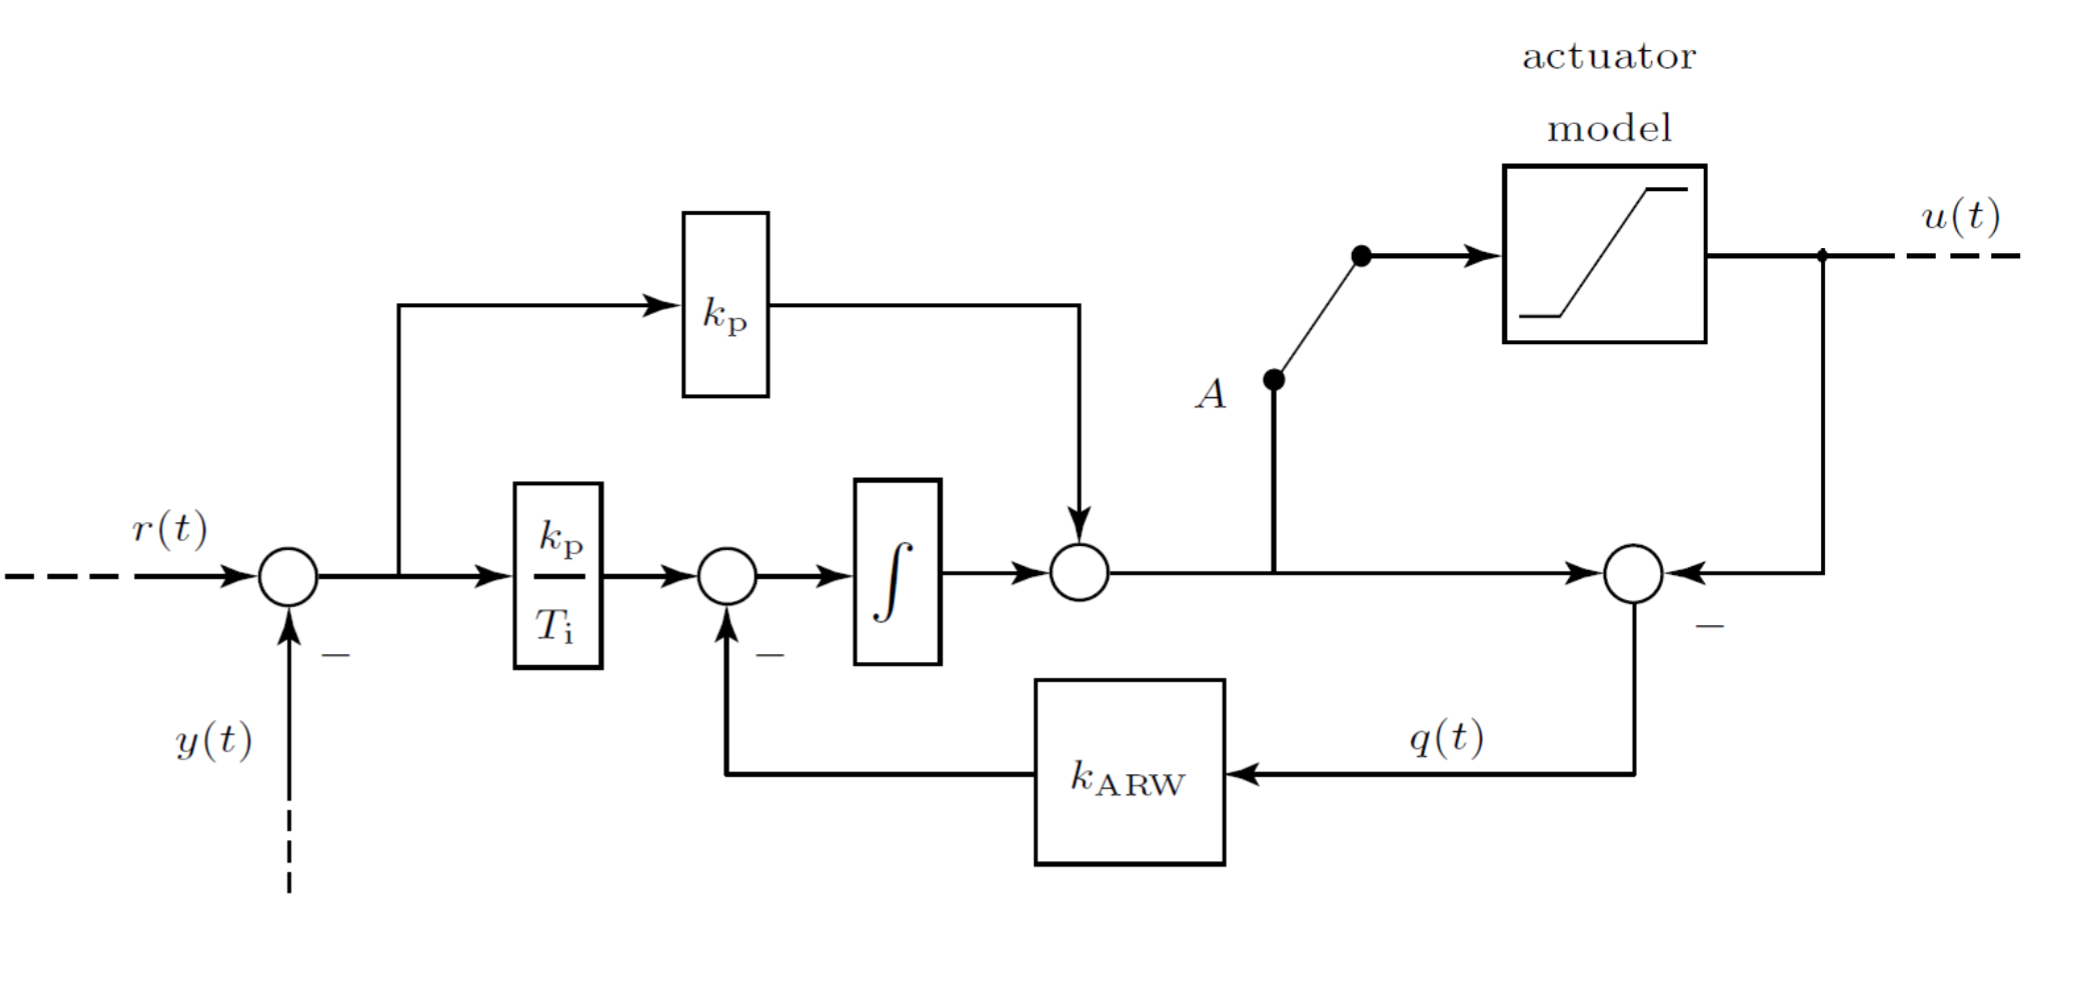
\includegraphics[width=0.8\columnwidth]{arw1}
\end{center}
\caption{Anti-Reset Windups' structure.}
\end{figure}


\begin{figure}[H]
\begin{center}
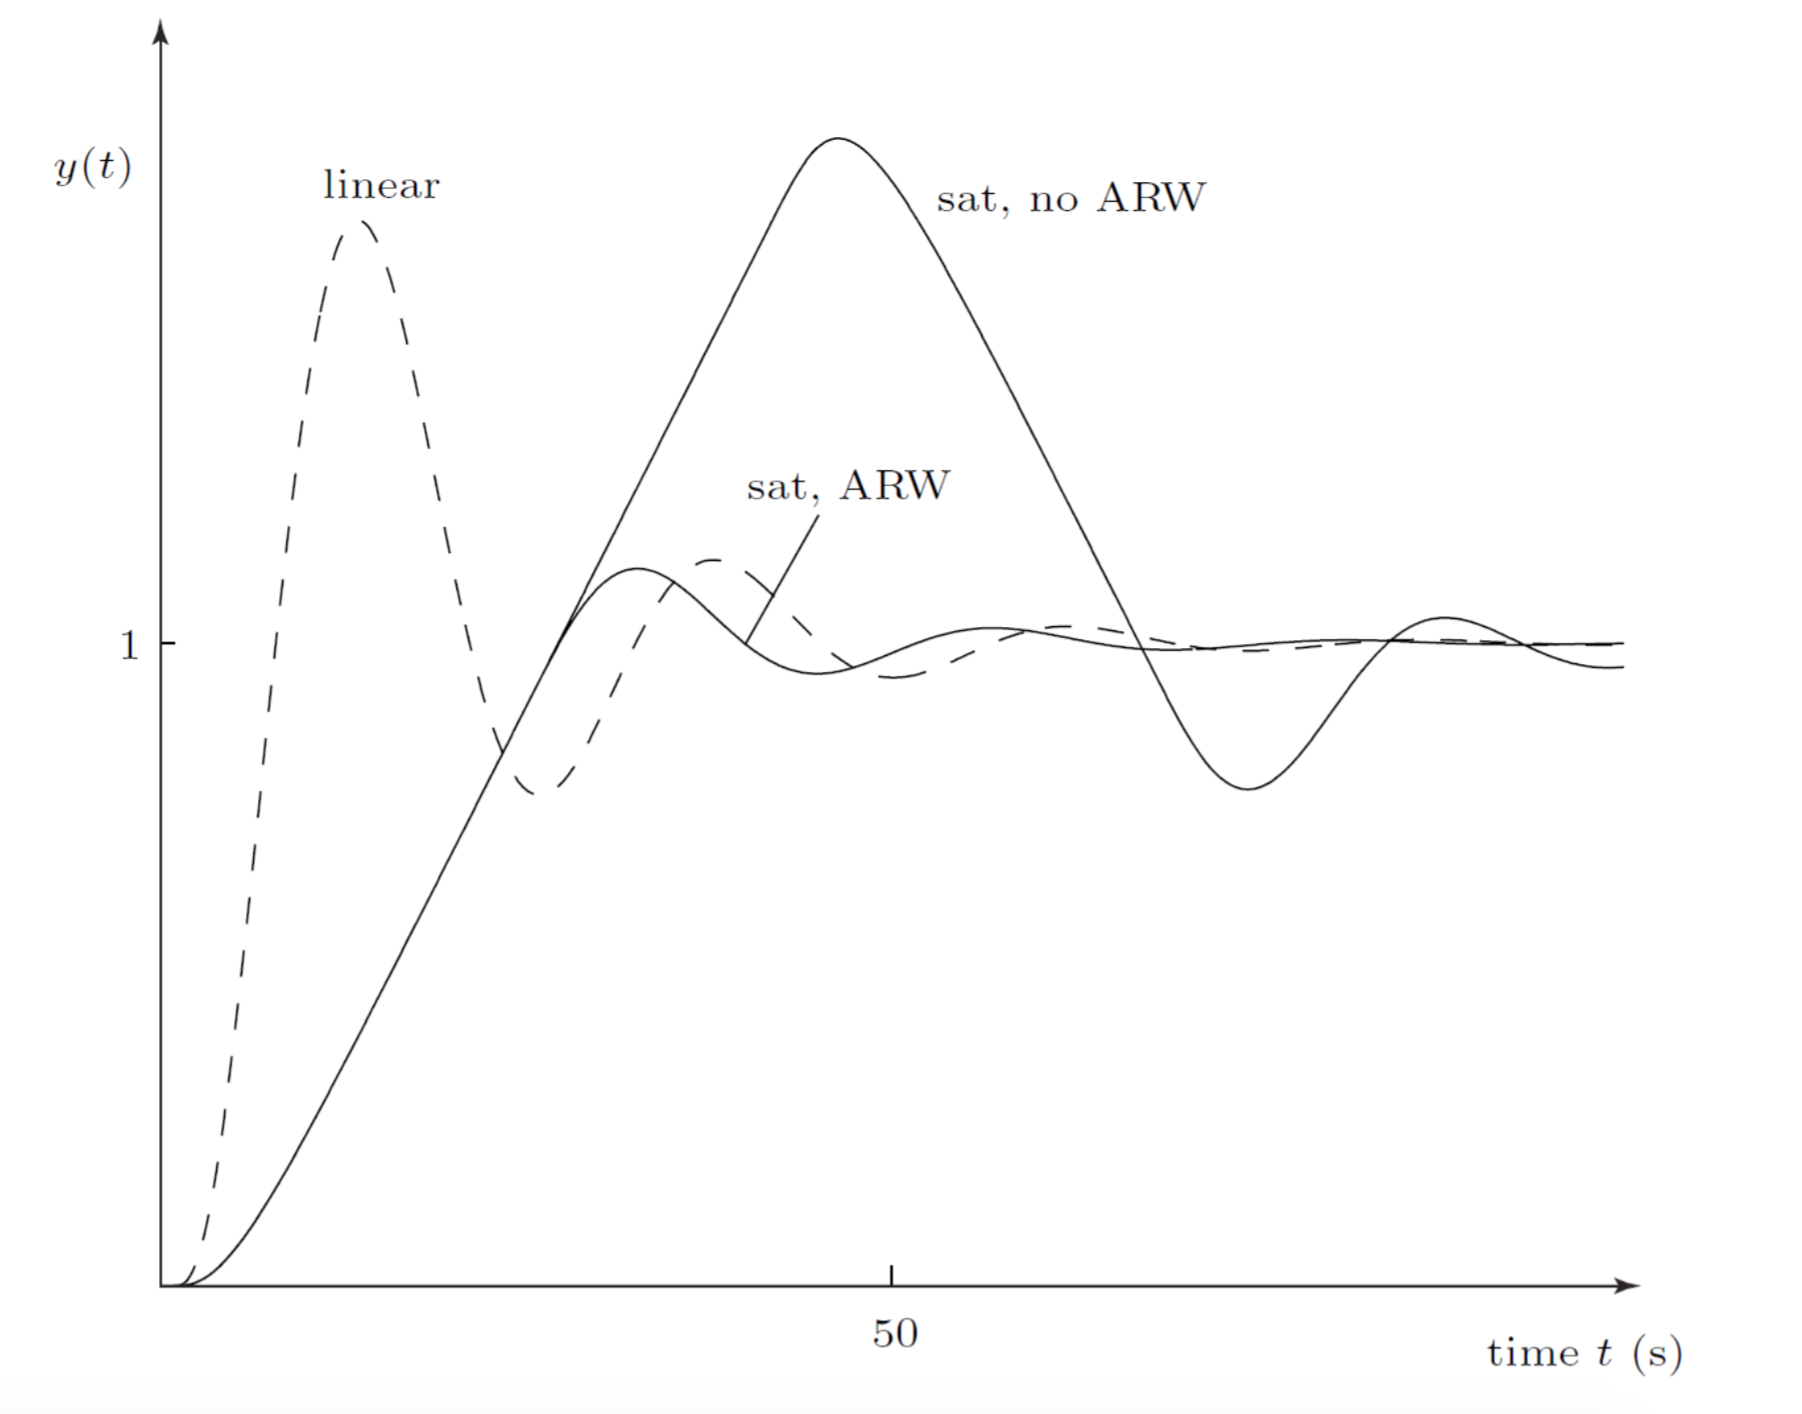
\includegraphics[width=0.6\columnwidth]{arw2}
\end{center}
\caption{Effects of the Anti-Reset Windups.}
\label{fig:osc}
\end{figure}
\newpage
\subsubsection{Examples}
\begin{bsp}

The plant 
$$P(s)=e^{-s}.$$
should be controlled with the PI controller
$$C(s)=0.2+\frac{1}{2s}.$$
An input limitation/saturation is given as
\begin{equation*}
u_b(t)
\begin{cases}
0.1, &if \ u(t)\geq 0.1\\
u(t), &if \ |u(t)|<0.1\\
-0.1, &if \ u(t)\leq 0.1.
\end{cases}
\end{equation*}

\begin{enumerate}[(a)]
\item Draw the signals $y(t)$, $u(t)$, $u_b(t)$ in the given diagram.
\item Which problem can be noticed in this problem? How could one solve this problem?
\end{enumerate}

\begin{figure}[H]
\begin{center}
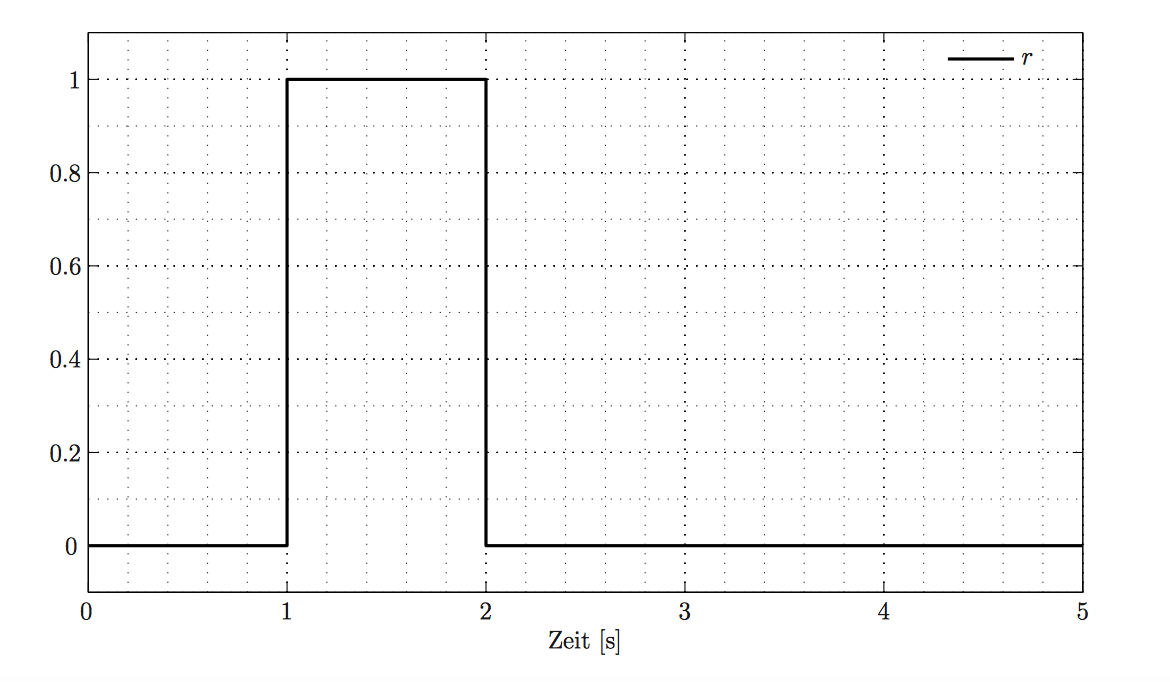
\includegraphics[width=0.9\columnwidth]{ex}
\end{center}
\caption{Diagram for the drawing. The signal $r(t)$ is given.}
\label{fig:osc}
\end{figure}
\newpage
\begin{lsg} 
\
\begin{enumerate}[(a)]
\item 
\end{enumerate}

First of all, we refer to a classical feedback loop with saturation (see Figure \ref{fig:sat}). \\ For the rest of the calculations, please refer to Figure \ref{fig:sol}
\end{lsg}



\begin{figure}[H]
\begin{center}
\begin{tikzpicture}[auto,node distance=2.5cm]%[auto, node distance=2cm,>=latex']
    \node [input, name=input] {};
    \node [sum, right of=input] (sum) {};
    \node [block, right of=sum] (controller) {$C(s)$};
    \node [block, right of=controller] (max) {
    \begin{tikzpicture}
    \begin{axis} [scale=.12,axis lines=middle,enlargelimits,xtick={0},ytick={0}]
        \addplot[domain=-1:-.48,color=black,smooth]{-.5};
        \addplot[domain=-.5:.5,color=black,smooth]{x};
        \addplot[domain=.48:1,color=black,smooth]{.5};
    \end{axis}\end{tikzpicture}
    };
    
    \node [block, right of=max] (system) {$P(s)$};
    \node [output, right of=system] (output) {};
    
    \draw [->] (input) -- node {$r$} (sum);
    \draw [->] (sum) -- node {$e$} (controller);
    \draw [->] (controller) -- node[] {$u$} (max);
    \draw [->] (max) -- node[] {${u_b}$} (system);
    \draw [->] (system) --  node[name=y] {$y$} (output);
    
    \draw [->] (y)   |-    (2.5cm,-1.5cm) --++  (sum) node[right,pos=0.98] {$-$}  ;
\end{tikzpicture}
\end{center}
\caption{Actuator Saturation.} 
\label{fig:sat}
\end{figure}

First of all, let's define how one can get $u(t)$. From the very definition:
$$U(s)=C(s)\cdot E(s).$$
This holds in frequency domain. If we want to draw a diagram in time domain, we have to compute the inverse Laplace transform of $U(s)$:
\begin{equation*}
\begin{split}
u(t)=\mathcal{L}^{-1}(U(s))&=\mathcal{L}^{-1}(C(s)\cdot E(s))\\
&=\mathcal{L}^{-1}(0.2\cdot E(s) +\frac{1}{2} \cdot \frac{1}{s} \cdot E(s)).
\end{split}
\end{equation*}
With the known Laplace inversions it follows
\begin{equation*}
u(t)=\mathcal{L}^{-1}(0.2\cdot E(s) +\frac{1}{2} \cdot \frac{1}{s} \cdot E(s))=0.2\cdot e(t)+\frac{1}{2}\int_0^t e(\tau)d\tau.
\end{equation*}

Now, let's analyze and draw the signals: we do this in intervals, in order to track every signals' change.
\begin{itemize}
\item $t\in [0,1]$
\end{itemize}
The reference signal $r$ is zero and so all the other signals.
\begin{itemize}
\item $t\in [1,2]$
\end{itemize}
Since the plant is a delay element of 1 second ($e^{-s}$), the output $y(t)$ would be still 0. This means that in this interval, the error is $e(t)=r(t)-y(t)=1$. We use this information to get the behaviour of $u(t)$:
\begin{equation*}
\begin{split}
u(t)&=0.2\cdot e(t) +\frac{1}{2} \int_0^te(\tau)d\tau\\
&=0.2\cdot 1 + \frac{1}{2} \cdot \int_1^t 1 d \tau\\
&= 0.2+ 0.5 \cdot (t-1).
\end{split}
\end{equation*}
In order to draw this, we evaluate $u(t)$ at $t=1$ and $t=2$. It holds
\begin{equation*}
\begin{split}
u(1)&=0.2,\\
u(2)&=0.7.\\
\end{split}
\end{equation*}
So, $u(t)$ is an increasing linear function from 0.2 to 0.7. \\
Since $u_b(t)$ is a function of $u(t)$, we can now find its shape: since $u(t)>0.1$ in the whole interval, we use the definition and say $u_b(t)=0.1$ (constant value).

\begin{itemize}
\item $t\in [2,3)$
\end{itemize}
There should be a step in $y(t)$ here: this can be seen in 
$$y(t)=u_b(t-1)=0.1.$$
This means that the error $e(t)=r(t)-y(t)=-0.1.$ We use this information to get the behaviour of u(t):
\begin{equation*}
\begin{split}
u(t)&=0.2\cdot e(t) +\frac{1}{2} \int_0^te(\tau)d\tau\\
&=0.2\cdot (-0.1) + \frac{1}{2} \cdot \left(\int_1^2 1 d \tau + \int_2^t (-0.1) d \tau\right)\\
&= -0.02+ 0.5+ 0.5 \cdot (-0.1)\cdot (t-2)\\
&=0.48-0.05\cdot (t-2).
\end{split}
\end{equation*}
In order to draw this, we evaluate $u(t)$ at $t=2$ and $t=3$. It holds
\begin{equation*}
\begin{split}
u(2)&=0.48,\\
u(3)&=0.43.\\
\end{split}
\end{equation*}
So, $u(t)$ is a decreasing linear function from 0.48 to 0.43. \\
Since $u_b(t)$ is a function of $u(t)$, we can now find its shape: since $u(t)>0.1$ in the whole interval, we use the definition and say $u_b(t)=0.1$ (constant value).
\begin{itemize}
\item $t\in [3,5)$
\end{itemize}
The error remains $e(t)=r(t)-y(t)=-0.1.$ since $y(t)=u_b(t-1)=0.1$. We use this information to get the behaviour of u(t):
\begin{equation*}
\begin{split}
u(t)&=0.2\cdot e(t) +\frac{1}{2} \int_0^te(\tau)d\tau\\
&=0.2\cdot (-0.1) + \frac{1}{2} \cdot \left(\int_1^2 1 d \tau + \int_2^t (-0.1) d \tau\right)\\
&= -0.02+ 0.5+ 0.5 \cdot (-0.1)\cdot (t-2)\\
&=0.48-0.05\cdot (t-2).
\end{split}
\end{equation*}
which reads exactly the same as before. In order to draw this, we evaluate $u(t)$ at $t=2$ and $t=3$. It holds
\begin{equation*}
\begin{split}
u(3)&=0.43\\
u(5)&=0.33.\\
\end{split}
\end{equation*}
So, $u(t)$ is the same decreasing linear function as before. \\ Since $u_b(t)$ is a function of $u(t)$, we can now find its shape: since $u(t)>0.1$ in the whole interval, we use the definition and say $u_b(t)=0.1$ (constant value).


\begin{figure}[H]
\begin{center}
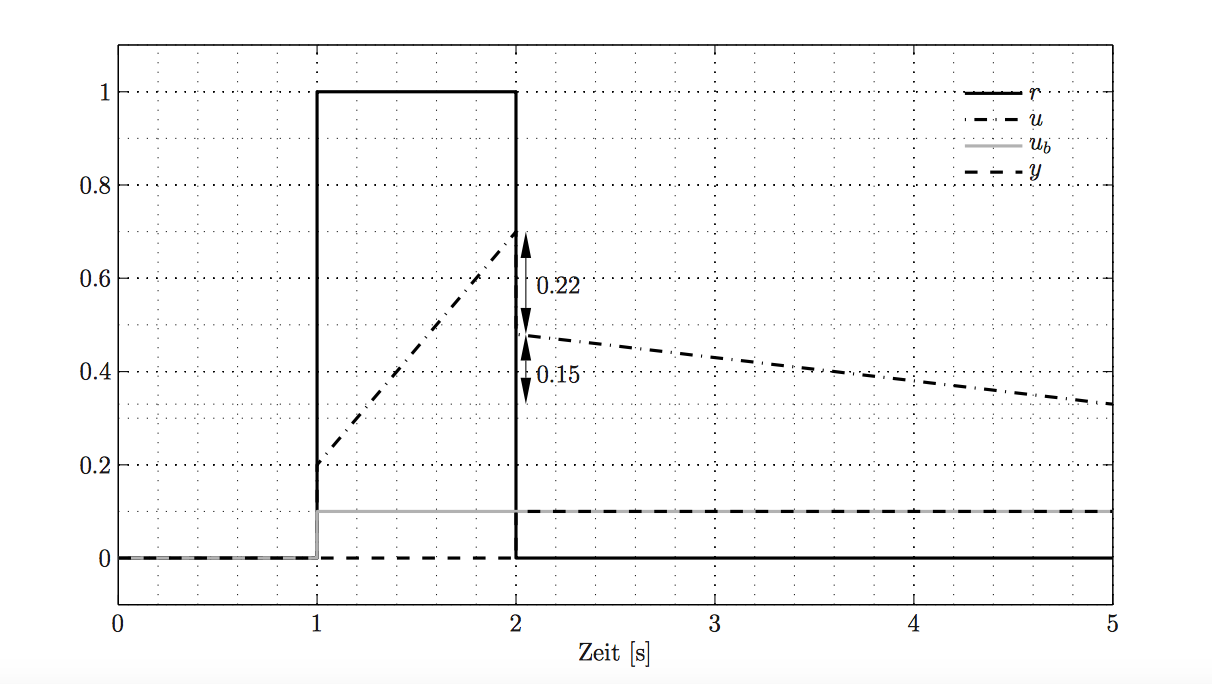
\includegraphics[width=0.9\columnwidth]{sol}
\end{center}
\caption{Solution.}
\label{fig:sol}
\end{figure}

\begin{enumerate}[(b)]
\item
\end{enumerate}
This example, shows the problem that is introduced by saturation. The from the controller asked input $u(t)$ is bigger than the real feasible input $u_b(t)$. This creates the windup situation and we can use an ARW structure to avoid this. 

\end{bsp}
\newpage
\subsection{Digital Control}
\subsubsection{Signals and Systems}
A whole course is dedicated to this topic (see Signals and Systems of professor D'Andrea). A \textit{signal} is a function of time that represents a physical quantity. \\ \textbf{Continuous-Time} signals are described by a function $x(t)$ such that this takes continuous values. \\\textbf{Discrete-Time} Signals are described by a function $x[n]=x(n\cdot T_s)$ where $T_s$ is the \textbf{sampling time}. The \textbf{sampling frequency} is defined as $f_s=\frac{1}{T_s}$. \\
One can see the difference between the two descriptions in Figure \ref{fig:ctdt}.


\begin{figure}[h]
\begin{center}\begin{tikzpicture}
 \begin{axis} [scale=1,axis lines=middle,enlargelimits,xtick={0},ytick={0},xlabel={$t$},ylabel={$x(t)$}]
    \addplot[domain=0:2,color=black,smooth]{ln(x+1)-.5*x*x+0.2*x^3};
        
    \addplot[color=black,mark=*, mark options={fill=black}]
    coordinates {(1,0)(1,0.393147)};
    \addplot[color=black,mark=*, mark options={fill=black}]
    coordinates {(.5,0)(.5,0.305465)};
    \addplot[color=black,mark=*, mark options={fill=black}]
    coordinates {(.25,0)(.25,0.195019)};
    \addplot[color=black,mark=*, mark options={fill=black}]
    coordinates {(.75,0)(.75,0.362741)};
    \addplot[color=black,mark=*, mark options={fill=black}]
    coordinates {(1.25,0)(1.25,0.420305)};
    \addplot[color=black,mark=*, mark options={fill=black}]
    coordinates {(1.5,0)(1.5,0.466291)};
    \addplot[color=black,mark=*, mark options={fill=black}]
    coordinates {(1.75,0)(1.75,0.552226)};
    \addplot[color=black,mark=*, mark options={fill=black}]
    coordinates {(2,0)(2,0.698612)};
\end{axis}\end{tikzpicture}\end{center}
\caption{Continuous-Time versus Discrete-Time representation}
\label{fig:ctdt}
\end{figure}

\subsubsection*{Advantages of Discrete-Time analysis}
\begin{itemize}
\item Calculations are easier. Moreover, integrals become sums and differentiations become finite differences. 
\item One can implement complex algorithms.
\end{itemize}



\subsubsection*{Disadvantages of Discrete-Time analysis}
\begin{itemize}
\item The sampling introduces a delay in the signal ($\approx e^{-\frac{sT_s}{2}}$)
\item The informations between two samplings, that is between $x[n]$ and $x[n+1]$ is lost.
\end{itemize}
Every real-world signal is some sort of discrete-time signal.

\subsubsection{Discrete-Time State-Space Description}
If in continuous-time we have to deal with differential equations, in discrete-time we have to work with \textbf{difference equations}: the discrete-time state-space description is very similar to the continuous-time one: 
\begin{equation}
\begin{split}
x[k+1]&=A\cdot x[k] +b\cdot u[k]\\
y[k]&=c\cdot x[k] + d \cdot u[k].
\end{split}
\end{equation}
\subsubsection*{Lyapunov Stability}
A system is \textbf{asymptotically stable} if and only if 
\begin{equation}
|\lambda_i|<1 \ \forall i.
\end{equation}
where $\lambda_i$ are the eigenvalues of $A$. This, in other words, means that the eigenvalues should remain inside the unity circle.
\subsubsection{Discrete-Time Control Systems}
Nowadays, controls systems are implemented in microcontroller or in microprocessors in discrete-time and really rarely (see the lecture \textit{Elektrotechnik II}) in continuous-time. Like defined, although the processes are faster and easier, the informations are still sampled and there is a certain loss of data.
\subsubsection*{Aliasing}
If the sampling frequency is chosed too low, i.e. one measures less times pro second, the signal can become poorly determined and the loss of information is too big to reconstruct it uniquely. This situation is called \textbf{aliasing} and one can find many examples of that in the real world. Let's take an easy example: you are finished with the summer's session and you are flying to Ibiza, to finally enjoy the sun after a summer at ETH. You decide to film the turbine of the plane because, although you are on holiday, you have an engineer's spirit. You arrive to Ibiza and as you get into your hotel room, you want you have a look at your film. The rotation you observe looks different to what it is supposed to be, and since you haven't drunk yet, there must be some scientific reason. In fact, the sampling frequency of your phone camera is much lower than the turning frequency of the turbine: this results in a loss of information and hence in a wrong perception of what is going on.\\ \\ 
Let's assume some signal 
\begin{equation}
x_1(t)=\cos(\omega \cdot t).
\end{equation}
After discretization, the sampled signal reads
\begin{equation}
x_1[n]=\cos(\omega \cdot T_s \cdot n)=\cos(\Omega \cdot n), \quad \Omega=\omega \cdot T_s.
\end{equation}
Let's assume a second signal
\begin{equation}
x_2(t)=\cos \left(\left(\omega +\frac{2\pi}{T_s}\right)\cdot t\right),
\end{equation}
where the frequency
\begin{equation}
\omega_2=\omega+\frac{2\pi}{T_s}.
\end{equation}
is given. The discretization of this second signal reads
\begin{equation}
\begin{split}
x_2[n]&=\cos \left( \left( \omega + \frac{2\pi}{T_s}\right) \cdot T_s \cdot n\right)\\
&=\cos \left( \omega \cdot T_s \cdot n+ 2\pi \cdot n \right)\\
&=\cos(\omega \cdot T_s \cdot n)\\
&=x_1[n].
\end{split}
\end{equation}
Although the two signals have different frequencies, they are equal when discretized. For this reason, one has to define an interval of \textit{good} frequencies, where aliasing doesn't occur. In particular it holds
\begin{equation}
|\omega|<\frac{\pi}{T_s}
\end{equation}
or
\begin{equation}
f<\frac{1}{2\cdot T_s} \Leftrightarrow f_s>2\cdot f_{max}.
\end{equation}
The maximal frequency accepted is $f=\frac{1}{2\cdot T_s}$ and is named \textbf{Nyquist Frequency}. In order to ensure good results, one uses in practice a factor of 10
\begin{equation}
f<\frac{1}{10\cdot T_s} \Leftrightarrow f_s>10\cdot f_{max}.
\end{equation}
For control systems the crossover frequency should follow
\begin{equation}
f_s\geq 10\cdot \frac{\omega_c}{2\pi}.
\end{equation}
\subsubsection*{Anti Aliasing Filter (AAF)}
The Anti Aliasing Filter is an \textbf{analog} filter and not a discrete one. In fact, we want to eliminate unwanted frequencies before sampling, because after that is \textit{too late} (see Figure \ref{fig:micro}). But how can one define unwanted frequencies? Those frequencies are normally the higher frequencies of a signal \footnote{Keep in mind: high signal frequency means problems by lower sampling frequency!}. Because of that, as AAF one uses normally a \textbf{low-pass filter}. This type of filter, \textit{lets} low frequencies \textit{pass} and blocks higher ones\footnote{This topic is exhaustively treated in the course Signals and Systems}. The mathematic formulation of a first-order low-pass filter is given by
\begin{equation}
lp(s)=\frac{k}{\tau\cdot s +1}.
\end{equation}
where $k$ is the gain and $\tau$ is the time constant of the system.
The drawback of such a filter is problematic: the filter introduces additional unwanted phase that can lead to unstable behaviours.


\subsubsection*{Analog to Digital Converter (ADC)}
At each discrete time step $t=k\cdot T$ the \textbf{ADC} converts a voltage $e(t)$ to a digital number following a sampling frequency. 
\subsubsection*{Microcontroller ($\mu P$)}
This is a discrete-time controller that uses the sampled discrete-signal and gives back a dicrete output.
\subsubsection*{Digital to Analog Converter (DAC)}
In order to convert back the signal, the \textbf{DAC} applies a \textbf{zero-order-hold (ZOH)}. This introduces an extra delay of $\frac{T}{2}$ (see Figure \ref{fig:del}).
\begin{figure}[h]
\centering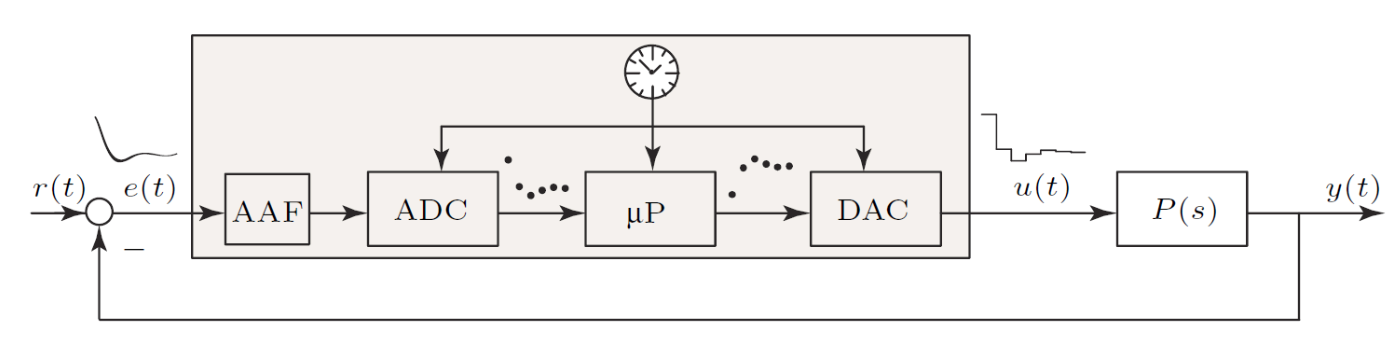
\includegraphics[width=0.9\columnwidth]{aaf}
\caption{Control Loop with AAF.}
\label{fig:micro}
\end{figure}

\begin{figure}[h]
\centering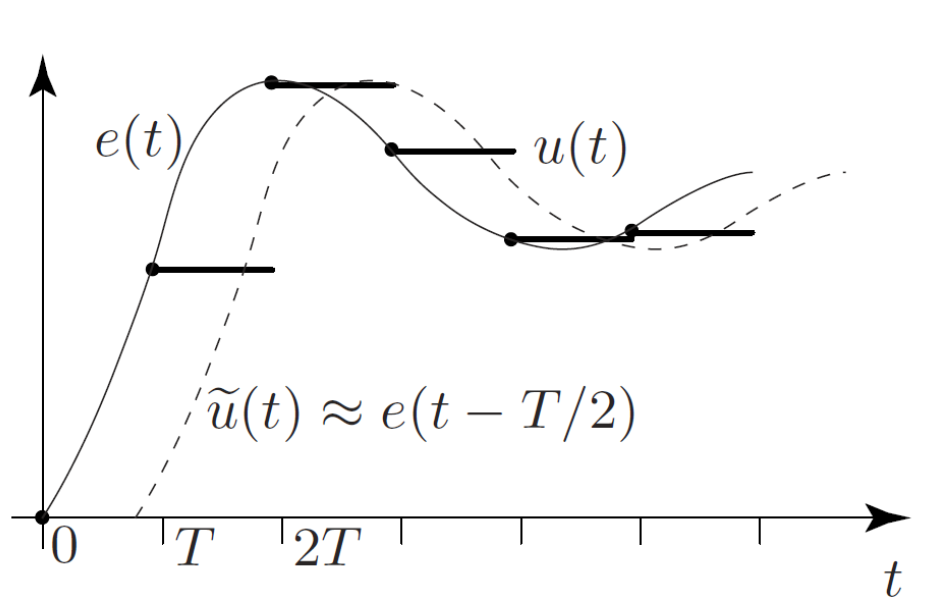
\includegraphics[width=0.7\columnwidth]{del}
\caption{Zero-Order-Hold.}
\label{fig:del}
\end{figure}

\subsubsection{Controller Discretization/Emulation}
Discrete-Time controllers can be defined by using the \textbf{z-Transform}: this transform method is to understand as some kind of Laplace transform (see the course \textit{Analysis III}). \\ In general, it holds
\begin{align}
y(t+T_s)&=y[n+1] \quad \Leftrightarrow\quad z\cdot Y(z).\\
\end{align}
The meaning of the variable $z$ can change with respect to the chosen discretization approach. Here, just discretization results are presented: if you are interested in the theory behind difference rules and discretization, have a look at courses like \textit{Computational Methods for Eng. Applications I/II}. A list of the most used transformations is:
\begin{center}\begin{tabular}{cll}\toprule
\textbf{Exakt} & $\displaystyle s=\frac{1}{T_s}\cdot \ln(z)$ &  $\displaystyle z=e^{s\cdot T_s}$ \\ \midrule
\textbf{Euler forward} & $\displaystyle s=\frac{z-1}{T_s}$ & $\displaystyle z=s\cdot T_s+1$ \\ \midrule
\textbf{Euler backward} & $\displaystyle s=\frac{z-1}{z\cdot T_s}$ &  $\displaystyle z=\frac{1}{1-s\cdot T_s}$ \\ \midrule
\textbf{Tustin} & $\displaystyle s=\frac{2}{T_s}\cdot \frac{z-1}{z+1}$ &
$\displaystyle z=\frac{1+s\cdot \frac{T_s}{2}}{1-s\cdot \frac{T_s}{2}}$ \\ \bottomrule
\end{tabular}\end{center}
The different approaches are results of different Taylor's approximations\footnote{As reminder: $e^x\approx 1+x$.}:

\begin{itemize}
\item Forward Euler:
\begin{equation}
z=e^{s\cdot T_s}\approx 1+s\cdot T_s.
\end{equation}
\item Backward Euler:
\begin{equation}
z=e^{s\cdot T_s}=\frac{1}{e^{-s\cdot T_s}}\approx\frac{1}{1-s\cdot T_s}.
\end{equation}
\item Tustin:
\begin{equation}
z=\frac{e^{s\cdot \frac{T_s}{2}}}{e^{-s\cdot \frac{T_s}{2}}}\approx\frac{1+s\cdot \frac{T_s}{2}}{1-s\cdot \frac{T_s}{2}}.
\end{equation}
\end{itemize}
In practice, the most used approach is the Tustin transformation, but there are cases where the other transformations could be useful.

\subsubsection*{Stability}
It is nice to investigate, how and if the stability conditions change in discretized systems. As a reminder, continuous-time systems are stable if their poles have a negative real part. Discrete-time systems are stable if their poles are bounded in the unity circle (see Figure \ref{fig:polemapping}).
With Euler Backward and Tustin the stability conditions remain the same; with Forward Euler it is however possible, that the systems becomes unstable (see Figure \ref{fig:polemapping}).

\begin{figure}[h!]
\centering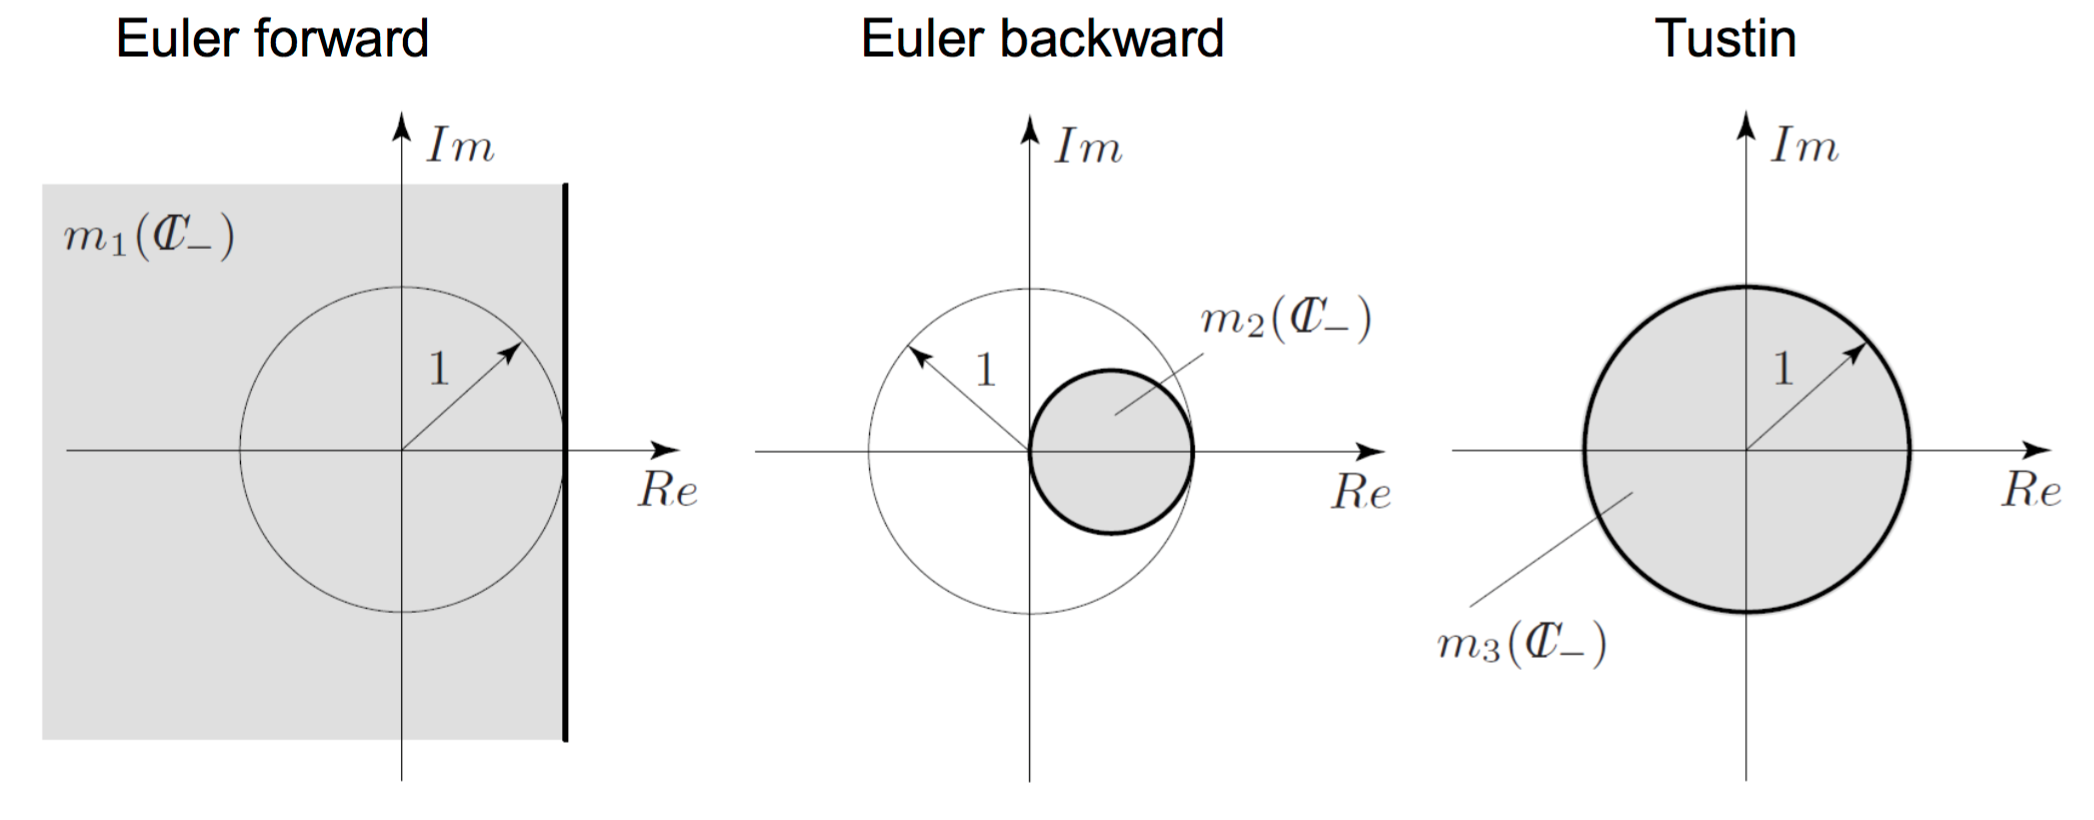
\includegraphics[width=0.75\columnwidth]{polemapping}
\caption{Pole mapping.}
\label{fig:polemapping}
\end{figure}
\pagebreak
\pagebreak

\subsubsection{Discrete Time Controller Synthesis}
As you learned in class, there are two ways to discretize systems: see Figure \ref{fig:methods}. \\
In the previous chapter, we learned how to emulate a system: in this chapter we learn the discrete time controller synthesis (direct synthesis).
\begin{figure}[h!]
\begin{center}
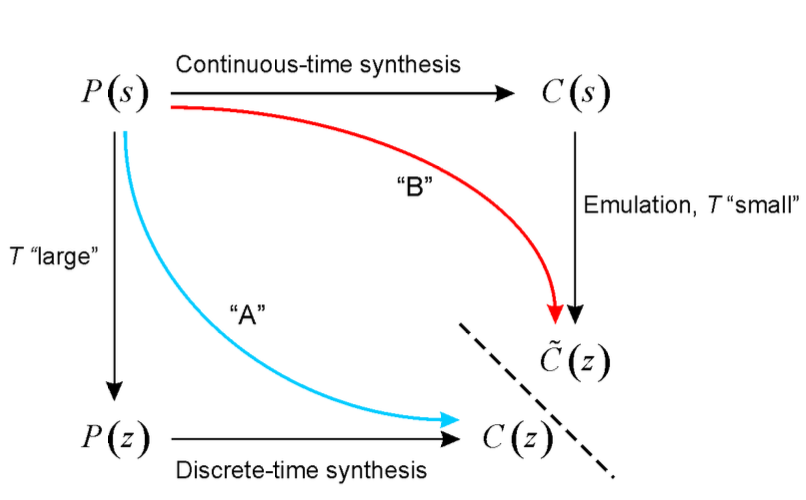
\includegraphics[width=0.65\columnwidth]{methods.png}
\caption{Emulation and Discrete time controller synthesis.}
\label{fig:methods}
\end{center}
\end{figure}
\begin{figure}[h!]
\begin{center}
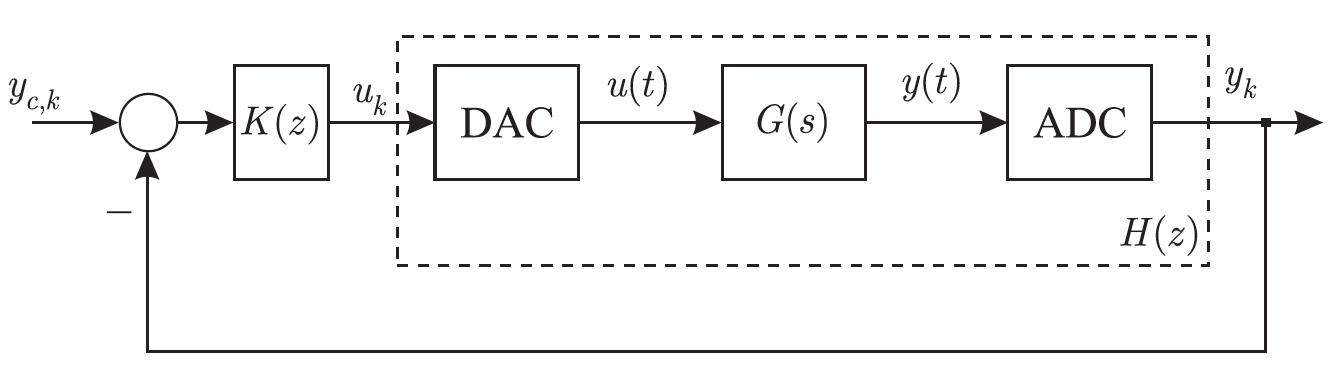
\includegraphics[width=0.85\columnwidth]{ex_3.png}
\caption{Discrete-time control loop.}
\label{fig:ex}
\end{center}
\end{figure}
\\
The general situation is the following: a control loop is given as in Figure \ref{fig:ex}. \\ The continuous time transfer function $G(s)$ is given. \\
We want to compute the equivalent discrete-time  transfer function $H(z)$. The loop is composed from a Digital-to-Analog Converter (DAC), the continuous-time transfer function $G(s)$ and an Analog to Digital Converter (ADC). \\
We want to reach a structure that looks like Figure \ref{fig:dis}.\\
The first thing to do, is to consider an input to analyze. What is usually chosen, is a \textbf{unit-step}
\begin{equation}
u(kT)=\{\hdots,0,1,1,\hdots\}.
\end{equation}
Since the $z-$Transform is defined as
\begin{equation}
X(z)=\sum_{n=0}^\infty x(n)\cdot z^{-n}
\end{equation}

we get for $u$
\begin{equation}
U(z)=1+z^{-1}+z^{-2}+z^{-3}+\hdots+ z^{-n}.
\end{equation}
This sum can be written as (see geometric series)
\begin{equation}
U(z)=\frac{1}{1-z^{-1}}.
\end{equation}
For $U(z)$ to be defined, this sum must converge. This can be verified by exploring the properties of the geometric series.
\subsubsection*{Recall: sum of geometric series}
Let $S_n$ denote the sum over the first $n$ elements of a geometric series:
\begin{equation*}
\begin{split}
S_n&=U_0+U_0\cdot a+U_0\cdot a^2+\hdots+U_0\cdot a^{n-1}\\
&=U_0\cdot (1+a+a^2+\hdots +a^{n-1}).
\end{split}
\end{equation*}
Then
\begin{equation*}
a\cdot S_n=U_0\cdot (a+a^2+a^3+\hdots +a^n)
\end{equation*}
and 
\begin{equation*}
S_n-a\cdot S_n=U_0\cdot (1-a^n),
\end{equation*}
which leands to
\begin{equation*}
S_n=U_0\cdot \frac{1-a^n}{1-a}.
\end{equation*}
From here, it can be seen that the limit for $n$ going to infinity convergese if and only if the absolute value of $a$ is smaller than one:
\begin{equation}
\lim_{n\rightarrow \infty}S_n=U_0\cdot \frac{1}{1-a}, \text{\textbf{iff} } |a|<1. 
\end{equation}
Therefore the limiting case $|a|=1=:r$ is called \textbf{radius of convergence}. The according \textbf{convergence criterion} is $|a|<r$. \\
$H(z)$ contains the converters: at first, we have the \textit{digital -to-analog} converter. The \textit{Laplace-Transform} of the unit-step reads generally
\begin{equation}
\frac{1}{s}.
\end{equation}
Hence, the transfer function before the \textit{analog-to-digital} converter reads
\begin{equation}
\frac{G(s)}{s}.
\end{equation}
In order to consider the \textit{analog-to-digital} converter, we have to apply the inverse Laplace transfrom to get
\begin{equation}
y(t)=\mathscr{L}^{-1}\left( \frac{G(s)}{s}\right).
\end{equation}
Through a $z-$ transform one can now get $Y(z)$. It holds
\begin{equation}
\begin{split}
Y(z)&=\mathscr{Z}\left(y(kT)\right)\\
&=\mathscr{Z}\left( \mathscr{L}^{-1}\left( \frac{G(s)}{s}\right) \right).
\end{split}
\end{equation}
The transfer function is then given as
\begin{equation}
H(z)=\frac{Y(z)}{H(z)}.
\end{equation}





\begin{figure}[htbp]
\begin{center}
\begin{tikzpicture}[auto,node distance=2.5cm]%[auto, node distance=2cm,>=latex']
    \node [input, name=input] {};
    \node [sum, right of=input] (sum) {};
    \node [block, right of=sum] (controller) {$K(z)$};
   % \node [sum, right of=controller,pin={[pinstyle]above:$w$}] (sum1) {};
    \node [block, right of=controller] (system) {$H(z)$};
  %  \node [sum, right of=system,pin={[pinstyle]above:$d$}] (sum2) {};
    \node [output, right of=system] (output) {};
    
    \draw [->] (input) -- node {$y_r$} (sum);
    \draw [->] (sum) -- node {$\varepsilon(z)$} (controller);
 %   \draw [->] (controller) -- node[] {} (controller);
    \draw [->] (controller) -- node[] {$U(z)$} (system);
  %  \draw [->] (system) -- node[] {} (system);
    \draw [->] (system) -- node[name=y] {$Y(z)$} (output);
    
   \node [sum, below of=y,pin={[pinstyle]right:$n=0$}] (sum3) {};
    
   \draw [->] (y) -- node[] {} (sum3);
    \draw [->] (sum3) -| node[right,pos=0.98] {$-$} (sum);
\end{tikzpicture}
\caption{Discrete Syhtesis.}
\label{fig:dis}
\end{center}
\end{figure}
\vfill
\pagebreak
\newpage



\subsubsection{Examples}
\begin{bsp} Show that the stability conditions of a system remain the same if stable continuous-time poles are mapped to discrete-time poles.
\newpage 
\begin{lsg}
\
 If one looks at Tustin it holds
\begin{equation*}
\begin{split}
z&=\frac{1+s\cdot \frac{T_s}{2}}{1-s\cdot \frac{T_s}{2}}\\
&=\frac{1+(x+i\cdot y)\cdot \frac{T_s}{2}}{1-(x+i\cdot y)\cdot \frac{T_s}{2}}\\
&=\frac{1+x\cdot \frac{T_s}{2}+i\cdot y\cdot \frac{T_s}{2}}{1-x\cdot \frac{T_s}{2}-i\cdot y\cdot \frac{T_s}{2}}.
\end{split}
\end{equation*}
If we compute the modulus, we get
\begin{equation*}
|z|=\sqrt{\frac{(1+x\cdot \frac{T_s}{2})^2+y^2\cdot(\frac{T_s}{2})^2}{(1-x\cdot \frac{T_s}{2})^2+y^2\cdot(\frac{T_s}{2})^2}}.
\end{equation*}
Since the continuous-time system should be stable, it should hold
$$x<0$$
This means
\begin{equation*}
(1+x\cdot \frac{T_s}{2})^2+y^2\cdot(\frac{T_s}{2})^2<(1-x\cdot \frac{T_s}{2})^2+y^2\cdot(\frac{T_s}{2})^2,
\end{equation*}
and so $$|z|<1.$$ The discrete-time is therefore stable.
\end{lsg}
\end{bsp}

\newpage

\begin{bsp}
One of your colleagues has developed the following continuous-time controller for a continuous-time plant
\begin{equation*}
C(s)=\frac{2s+1}{s+\alpha}
\end{equation*}
where $\alpha \in \mathbb{R}$ is a tuning factor.
\begin{enumerate}[(a)]
\item You now want to implement the controller on a microprocessor using the \textbf{Euler backward} emulation approach. What is the resulting function $C(z)$ for a generic sampling time $T \in \mathbb{R^+}$?
\item What is the range of the tuning factor $\alpha$ that produces an asymptotically stable discrete.time controller when applying the Euler backward emulation approach?
\item What is the condition on $\alpha$ to obtain an asymptotically stable continuous-time controller $C(s)$ and an asymptotically stable discrete-time controller $C(z)$ using the Euler backward emulation approach?
\end{enumerate}

\newpage
\begin{lsg}
\
\begin{enumerate}[(a)]
\item The Euler backward emulation approach reads
\begin{equation*}
s=\frac{z-1}{T\cdot z}.
\end{equation*}
If one substitutes this into the transfer function of the continuous-time controller, one gets
\begin{equation*}
\begin{split}
C(z)&=\frac{2\cdot \frac{z-1}{T\cdot z}+1}{\frac{z-1}{T\cdot z}+\alpha}\\
&=\frac{z\cdot (2+T)-2}{z\cdot(1+\alpha \cdot T)-1}.
\end{split}
\end{equation*}
\item The controller $C(z)$ is asymptotically stable if its pole $\pi_d$ fulfills the condition
$$|\pi_d|<1.$$
The pole reads
\begin{equation*}
\begin{split}
z\cdot(1+\alpha \cdot T)-1&=0\\
\pi_d &= \frac{1}{1+\alpha \cdot T}.
\end{split}
\end{equation*}
This, together with the condition for stability gives
\begin{equation*}
-1<\frac{1}{1+\alpha \cdot T}<1 \Rightarrow \alpha >0 \text{ or } \alpha<-\frac{2}{T}.
\end{equation*}
\item For $C(s)$ to be asymptotically stable, its pole $\pi_c=-\alpha$ must lie in the left half of the complex plane:
\begin{equation*}
\text{Re}\{ \pi_c \}<0 \Rightarrow \alpha>0.
\end{equation*}
Together with the results from (b), the condition on $\alpha$ is $\alpha>0$.




\end{enumerate}

\end{lsg}

\end{bsp}



\newpage

\begin{bsp}
\
\begin{enumerate}[(a)]
\item Choose all the signals that can be sampled without aliasing. The sampling time is $T_s=1s$.
 \begin{todolist}
  \item $x(t)=\cos(4\pi\cdot t)$.
  \item $x(t)=\cos(4\pi\cdot t +\pi)$.
  \item $x(t)=2\cdot \cos(4\pi\cdot t+ \pi)$.
  \item  $x(t)=\cos(0.2\pi\cdot t)$.
  \item  $x(t)=\cos(0.2\pi\cdot t + \pi)$.
  \item  $x(t)=3\cdot \cos(0.2\pi\cdot t + \pi)$.
  \item $x(t)=\cos(\pi\cdot t)$.
  \item $x(t)=\cos(\pi\cdot t+\pi)$.
  \item $x(t)=2\cdot \cos(\pi\cdot t+\pi)$.
  \item $x(t)=\cos(0.2\pi\cdot t)+\cos(4\pi\cdot t)$.
  \item $x(t)=\sin(0.2\pi\cdot t)+\sin(0.4\pi\cdot t)$.
  \item $x(t)=\sum_{i=1}^{100}\cos\left(\frac{2\pi}{i+1}\cdot t \right)$.
  \item  $x(t)=\sum_{i=1}^{100}\cos\left(\frac{2\pi}{i+2}\cdot t \right)$.
  \end{todolist}
  
\item The signal
$$x(t)=2\cdot \cos(20\cdot \pi \cdot t+\pi)+\cos(40\cdot \pi \cdot t)+\cos(30\cdot \pi \cdot t).$$
is sampled with sampling frequency $f_s$. What is the minimal $f_s$ such that no aliasing occurs?
\end{enumerate}
\newpage
\begin{lsg}
\
\begin{enumerate}[(a)]
\item

 \begin{todolist}
  \item $x(t)=\cos(4\pi\cdot t)$.
  \item $x(t)=\cos(4\pi\cdot t +\pi)$.
  \item $x(t)=2\cdot \cos(4\pi\cdot t+ \pi)$.
  \item [\done] $x(t)=\cos(0.2\pi\cdot t)$.
  \item [\done] $x(t)=\cos(0.2\pi\cdot t + \pi)$.
  \item [\done] $x(t)=3\cdot \cos(0.2\pi\cdot t + \pi)$.
  \item $x(t)=\cos(\pi\cdot t)$.
  \item $x(t)=\cos(\pi\cdot t+\pi)$.
  \item $x(t)=2\cdot \cos(\pi\cdot t+\pi)$.
  \item $x(t)=\cos(0.2\pi\cdot t)+\cos(4\pi\cdot t)$.
  \item [\done] $x(t)=\sin(0.2\pi\cdot t)+\sin(0.4\pi\cdot t)$.
  \item $x(t)=\sum_{i=1}^{100}\cos\left(\frac{2\pi}{i+1}\cdot t \right)$.
  \item [\done] $x(t)=\sum_{i=1}^{100}\cos\left(\frac{2\pi}{i+2}\cdot t \right)$.
  \end{todolist}
\textbf{Explanation:}\\
If one goes back to the definition of the ranges to ensure no aliasing occurs, one gets the formula
$$f<\frac{1}{2\cdot T_s}.$$
In this case the condition reads
$$f<\frac{1}{2\cdot 1s}=0.5Hz.$$
One can read the frequency of a signal from its formula: the value that multiplies $t$ is $\omega$ and $$\frac{\omega}{2\pi}=f.$$ The first three signals have $$f=\frac{4\pi}{2\pi}=2Hz.$$ which is greater than $0.5Hz$. Moreover, additional phase and gain don't play an important role in this sense. The next three signals have a frequency of $$f=\frac{0.2\pi}{2\pi}=0.1Hz.$$ that is lower than $0.5Hz$ and hence perfect, in order to not encounter aliasing. The next three signals have the critical frequency and theoretically speaking, one sets this as already aliased. The reason for that is that the Nyquist theorem sets a strict $<$ in the condition. \\
For the next two signals a special procedure applies: if one has a combination of signals, one has to look at the bigger frequency of the signal. In the first case this reads $2Hz$, that exceeds the limit frequency. In the second case this reads $0.2Hz$, that is acceptable. The last two cases are a general form of combination of signals. The leading frequency of the first sum, decreases with $\frac{1}{i+1}$ and has its biggest value with $i=1$, namely $0.5Hz$. This is already at the limit frequency, hence not acceptable. The leading frequency of the second sum, decreases with $\frac{1}{i+2}$ and has its biggest value with $i=1$, namely $0.33Hz$. This is lower that the limit frequency, hence acceptable.
\item The general formula reads
$$f_s>2\cdot f_{max}.$$
Here it holds
$$f_{max}=\frac{40\pi}{2\pi}=20Hz.$$
It follows
$$f_s>2\cdot 20Hz=40Hz.$$
  \end{enumerate}
\end{lsg}

\end{bsp}
\newpage
\begin{bsp}
\
\begin{enumerate}[(a)]
\item For which $A$ and $B$ is the system asymptotically stable?
 \begin{todolist}
 \item $A=\begin{pmatrix}
 1&2\\
 1&2\\
 \end{pmatrix}$, $B=\begin{pmatrix} 
1\\2
\end{pmatrix}$.

 \item $A=\begin{pmatrix}
 -1&-2\\
 -1&-2\\
 \end{pmatrix}$, $B=\begin{pmatrix} 
1\\2
\end{pmatrix}$.

 \item $A=\begin{pmatrix}
 0&0\\
 0&0\\
 \end{pmatrix}$, $B=\begin{pmatrix} 
0.1\\0
\end{pmatrix}$.

 \item $A=\begin{pmatrix}
 -1&-2\\
 1&-0.5\\
 \end{pmatrix}$, $B=\begin{pmatrix} 
1\\2
\end{pmatrix}$.

 \item $A=\begin{pmatrix}
 -1&-2\\
 0&-0.5\\
 \end{pmatrix}$, $B=\begin{pmatrix} 
1\\2
\end{pmatrix}$.

 \item $A=\begin{pmatrix}
 1&-2\\
 0&0.5\\
 \end{pmatrix}$, $B=\begin{pmatrix} 
1\\2
\end{pmatrix}$.
 \item $A=\begin{pmatrix}
 -0.1&-2\\
 0&-0.5\\
 \end{pmatrix}$, $B=\begin{pmatrix} 
1\\2
\end{pmatrix}$.
 \item $A=\begin{pmatrix}
 -0.1&-2\\
 0&-0.5\\
 \end{pmatrix}$, $B=\begin{pmatrix} 
0.1\\0
\end{pmatrix}$.

 \item  $A=\begin{pmatrix}
 0.1&-2\\
 0&0.5\\
 \end{pmatrix}$, $B=\begin{pmatrix} 
1\\2
\end{pmatrix}$.

 \item $A=\begin{pmatrix}
 0.1&-2\\
 0&0.5\\
 \end{pmatrix}$, $B=\begin{pmatrix} 
0.1\\0
\end{pmatrix}$.

 \end{todolist}
\item The previous exercise can be solved independently of $B$.
\begin{todolist}
\item True.
\item False.
\end{todolist}
\end{enumerate}
\newpage
\begin{lsg}
\
\begin{enumerate}[(a)]
\item 

\begin{todolist}
 \item $A=\begin{pmatrix}
 1&2\\
 1&2\\
 \end{pmatrix}$, $B=\begin{pmatrix} 
1\\2
\end{pmatrix}$.

 \item $A=\begin{pmatrix}
 -1&-2\\
 -1&-2\\
 \end{pmatrix}$, $B=\begin{pmatrix} 
1\\2
\end{pmatrix}$.

 \item [\done] $A=\begin{pmatrix}
 0&0\\
 0&0\\
 \end{pmatrix}$, $B=\begin{pmatrix} 
0.1\\0
\end{pmatrix}$.

 \item $A=\begin{pmatrix}
 -1&-2\\
 1&-0.5\\
 \end{pmatrix}$, $B=\begin{pmatrix} 
1\\2
\end{pmatrix}$.

 \item $A=\begin{pmatrix}
 -1&-2\\
 0&-0.5\\
 \end{pmatrix}$, $B=\begin{pmatrix} 
1\\2
\end{pmatrix}$.

 \item [\done] $A=\begin{pmatrix}
 -0.1&-2\\
 0&-0.5\\
 \end{pmatrix}$, $B=\begin{pmatrix} 
1\\2
\end{pmatrix}$.
 \item [\done]$A=\begin{pmatrix}
 -0.1&-2\\
 0&-0.5\\
 \end{pmatrix}$, $B=\begin{pmatrix} 
0.1\\0
\end{pmatrix}$.

 \item [\done] $A=\begin{pmatrix}
 0.1&-2\\
 0&0.5\\
 \end{pmatrix}$, $B=\begin{pmatrix} 
1\\2
\end{pmatrix}$.

 \item [\done]$A=\begin{pmatrix}
 0.1&-2\\
 0&0.5\\
 \end{pmatrix}$, $B=\begin{pmatrix} 
0.1\\0
\end{pmatrix}$.
\end{todolist}
\textbf{Explanation:}\\
The eigenvalues of $A$ should fulfill
$$|\lambda_i|<1.$$
\item 
\
\begin{todolist}
\item [\done] True.
\item False.
\end{todolist}
\end{enumerate}

\end{lsg}


\end{bsp}
\newpage

\begin{bsp}
A continuous-time system with the following transfer function is considered:
\begin{equation*}
G(s)=\frac{9}{s+3}.
\end{equation*}
\begin{enumerate}[(a)]
\item Calculate the equivalent discrete-time transfer function $H(z)$. The latter is composed of a Digital-to-Analog Converter (DAC), the continuous-time transfer function $G(s)$ and an Analog-to-Digital Converter (ADC). Both converters, i.e. the DAC and ADC, have a sampling time $T_s=1s$.
\item Calculate the static error if a proportional controller $K(z)=k_p$ is used and the reference input $y_{c,k}$ is a step signal. \\
\textit{Hint: Heavyside with amplitude equal to 1.}
\end{enumerate}

\newpage
\begin{lsg}
\
\begin{enumerate}[(a)]
\item Rather than taking into account all the individuals elements which make up the continuous-time part of the system (DAC, plant, ADC), in a first step, these elements are lumped together and are represented by the discrete-time description $H(z)$. In this case, the discrete-time output of the system is given by
\begin{equation*}
Y(z)=H(z)\cdot U(z),
\end{equation*}
where $U(z)$ is the z-transform of the discrete input $u_k$ given to the system. Therefore , the discrete-time representation of the plant is given by the ratio of the output to the input
\begin{equation*}
H(z)=\frac{Y(z)}{U(z)}.
\end{equation*}
For the sake of convenience, $u_k$ is chosen to be the discrete-time \textit{Heaviside} function 
\begin{equation*}
\begin{cases}
u_k[k]=1, \ &k\geq 0\\
0,  \ &\text{else}.
\end{cases}
\end{equation*}
This input function needs to be z-transformed. Recall the definition of the z-transform 
\begin{equation*}
X(z)=\sum_{n=0}^\infty x(n)\cdot z^{-n}.
\end{equation*}
and applying it to the above equation, with the input $u_k$ gives ($u_k[k]=1$ for $k\geq 0$)
\begin{equation*}
\begin{split}
U(z)&=X(u_k)\\
&=\sum_{k=0}^\infty z^{-k}\\
&=\sum_{k=0}^\infty (z^{-1})^k.
\end{split}
\end{equation*}
For $U(z)$ to be defined, this sum must converge. Recalling the properties of geometric series one can see
\begin{equation*}
U(z)=\frac{1}{a-z^{-1}},
\end{equation*}
as long as the convergence criterion is satisfied, i.e. as long as $|z^{-1}|<1$ or better $|z|>1$. This signal is then transformed to continuous time using a zero-order hold DAC. The output of this transformation is again a Heaviside function $u_h(t)$. Since the signal is now in continuous time, the Laplace transform is used to for the analysis. The Laplace transform of the step function is well known to be
\begin{equation*}
\mathscr{L}(u_h(t))(s)=\frac{1}{s}=U(s).
\end{equation*}
The plant output in continuous time is given by
\begin{equation*}
\begin{split}
Y(s)&=G(s)\cdot U(s)\\
&=\frac{G(s)}{s}.
\end{split}.
\end{equation*}
After the plant $G(s)$, the signal is sampled and transformed into discrete time once more. Therefore, the z-transform of the output has to be calculated. However, the signal $Y(s)$ cannot be  transformed directly, since it is expressed in the frequency domain. Thus, first, it has to be transformed back into the time domain ($y(t)$) using the inverse Laplace transform, where it is them sampled every $t=k\cdot T$. The resulting series of samples $\{y[k]\}$ is then transformed back into the z-domain, i.e.
\begin{equation*}
Y(z)=X\left(\ \{ \mathscr{L}^{-1}\left(\frac{G(s)}{s} \right)(kT) \}\right).
\end{equation*}
To find the inverse Laplace transform of the output, its frequency domain representation is decomposed into a sum of simpler functions
\begin{equation*}
\begin{split}
\frac{G(s)}{s}&=\frac{9}{s\cdot (s+3)}\\
&=\frac{\alpha}{s}+\frac{\beta}{s+3}\\
&=\frac{s\cdot (\alpha + \beta)+3\cdot \alpha}{s\cdot (s+3)}.
\end{split}
\end{equation*}
The comparison of the numerators yields
$$\alpha=3,\ \ \beta=-3.$$
and thus
\begin{equation*}
\begin{split}
\frac{G(s)}{s}&=\frac{3}{s}-\frac{3}{s+3}\\
&=3\cdot \left(\frac{1}{s}-\frac{1}{s+3}\right).
\end{split}
\end{equation*}
Now the terms can be individually transformed with the result
\begin{equation*}
\begin{split}
\mathscr{L}^{-1}\left( \frac{G(s)}{s}\right)&=3\cdot \left(1-e^{-3t}\right) \cdot u_h(t)\\
&=y(t).
\end{split}
\end{equation*}
The z-transform of the output sampled at discrete time istants $y(kT)$ is given by
\begin{equation*}
\begin{split}
X(\{ y(kT)\})&=3\cdot \left[ \sum_{k=0}^{\infty}z^{-k}-\sum_{k=0}^\infty e^{-3kT} \cdot z^{-k}\right]\\
&=3\cdot \left[ \sum_{k=0}^{\infty}z^{-1}^k-\sum_{k=0}^\infty (e^{-3T} \cdot z^{-1})^k\right]\\
&=Y(z).
\end{split}
\end{equation*}
From above, the two necessary convergence criteria are known
\begin{equation*}
\begin{split}
|z^{-1}|<1 &\Rightarrow |z|>1\\
|e^{-3T}\cdot z^{-1}|&\Rightarrow |z|>|e^{-3T}|.
\end{split}
\end{equation*}
Using the above equations the output transfrom converges to (giben that the two convergence criteria are satisfied)
\begin{equation*}
Y(z)=3\cdot \left( \frac{1}{1-z^{-1}}-\frac{1}{1-e^{-3T}\cdot z^{-1}} \right).
\end{equation*}
Finally, the target transfer function $H(z)$ is given by
\begin{equation*}
\begin{split}
H(z)&=\frac{Y(z)}{U(z)}\\
&=(1-z^{-1})\cdot Y(z)\\
&=3\cdot \left( 1-\frac{1-z^{-1}}{1-e^{-3T}\cdot z^{-1}} \right)\\
&=3\cdot \frac{(1-e^{-3T})\cdot z^{-1}}{1-e^{-3T}\cdot z^{-1}}.
\end{split}
\end{equation*}
\item From the signal flow diagram, it can be seen that the error $\varepsilon(z)$ is composed of 
\begin{equation*}
\begin{split}
\varepsilon(z)&=Y_c(z)-Y(z)\\
&=Y_c(z)-H(z)\cdot K(z)\cdot \varepsilon(z)\\
&=\frac{Y_c(z)}{1+k_p\cdot H(z)}.
\end{split}
\end{equation*}
The input $y_c(t)$ is a discrete step signal, for which the z-transform was calculated in (a):
\begin{equation*}
Y_c(z)=\frac{1}{1+z^{-1}}.
\end{equation*}
Therefore, the error signal reads
\begin{equation*}
\varepsilon(z)=\frac{\frac{1}{1+z^{-1}}}{1+3\cdot k_p \cdot \frac{(1-e^{-3T})\cdot z^{-1}}{1-e^{-3T}\cdot z^{-1}}}.
\end{equation*}
To calculate the steady-state error, i.e. the error after infinite time, the discrete-time final value theorem\footnote{$\lim_{t\rightarrow \infty}\varepsilon (t)=\lim_{s\rightarrow 0}s\cdot \varepsilon (s)$} is used:
\begin{equation*}
\lim_{t\rightarrow \infty}\varepsilon (t)=\lim_{z\rightarrow 1}(1-z^{-1})\cdot \varepsilon(z),
\end{equation*}
but as $z$ goes to 1, so does $z^{-1}$ and thereforem 1 is substituted for each $z^{-1}$ in $\varepsilon (z)$ and the stati error becomes
\begin{equation*}
\varepsilon_\infty =\frac{1}{1+3\cdot k_p}.
\end{equation*}
Note that the error does not completely vanish but can be made smaller by increasing $k_p$. This is the same behaviour which would have been expected from a purely proportional controller in continuous time. To drive the static error to zero, a discrete-time integrator of the form $\frac{1}{T_i\cdot (1-z^{-1})}$ would be necessary.
\end{enumerate}

\end{lsg}
\newpage

\end{bsp}

\section{MIMO Systems}
MIMO systems are systems with multiple inputs and multiple outputs. In this chapter we will introduce some analytical tools to deal with those systems.
\subsection{System Description}
\subsubsection{State Space Descriprion}
The state-space description of a MIMO system is very similar to the one of a SISO system. \\ For a linear, time invariant MIMO system with $m$ input signals and $p$ output signals, it holds
\begin{equation}
 \begin{split}
 \dd{}{t} x(t) &= A \cdot x(t) + B \cdot u(t), \qquad x(t) \in \mathbb{R}^n, u(t) \in \mathbb{R}^m \\
 y(t) &= C \cdot x(t) + D \cdot u(t), \qquad \qquad \qquad y(t) \in \mathbb{R}^p
 \end{split}
 \label{eqMIMOstatespace}
 \end{equation}
where
\begin{equation} 
x(t) \in \mathbb{R}^{n\times 1},\ u(t) \in \mathbb{R}^{m\times 1},\ y(t) \in \mathbb{R}^{p\times 1},\ A \in \mathbb{R}^{n\times n}, \ B \in \mathbb{R}^{n\times m}, \ C \in \mathbb{R}^{p\times n}, \ D \in \mathbb{R}^{p\times m}.
\end{equation}
\begin{bmk}
The dimensions of the matrices $A,B,C,D$ are very important and they are a key concept to understand problems. \\ \\
The big difference from SISO systems is that $u(t)$ and $y(t)$ are here vectors and no more just numbers. For this reason $B,C,D$ are now matrices.
\end{bmk}
\subsubsection{Transfer Function}
One can compute the transfer function of a MIMO system with the well known formula
\begin{equation}
P(s)=C\cdot (s\cdot \mathbb{1}-A)^{-1}\cdot B+D.
\end{equation}
This is no more a scalar, but a $p\times m$-matrix. The elements of that matrix are rational functions. \\ Mathematically:
\begin{equation}
P(s)=\begin{pmatrix} P_{11}(s) & \cdots & P_{1m}(s) \\ \vdots & \ddots & \vdots \\ P_{p1}(s) & \cdots & P_{pm}(s)
\end{pmatrix}, \qquad P_{ij}(s)=\frac{b_{ij}(s)}{a_{ij}(s)}.
\end{equation}
Here $P_{ij}(s)$ is the transfer function from the $j$-th input to the $i$-th output.
\begin{bmk}
In the SISO case, the only matrix we had to care about was $A$. Since now $B$,$C$ are matrices, one has to pay attention to some mathematical properties: the matrix multiplication is not \textbf{commutative} ($A\cdot B \neq B\cdot A$). Since now $P(s)$ and $C(s)$ are matrices, it holds
\begin{equation}
L(s)=P(s)\cdot C(s)\neq C(s)\cdot P(s).
\end{equation}
\end{bmk}
Moreover, one can no more define the complementary sensitivity and the sensitivity as
\begin{equation}
T(s)=\frac{L(s)}{1+L(s)}, \ S(s)=\frac{1}{1+L(s)}.
\end{equation}
because no matrix division is defined. 
There are however similar expressions to describe those transfer functions: let's try to derive them.\\
We start from the standard control system's structure (see Figure \ref{fig:std}). \\
To keep things general, let's say the plant $P(s) \in \mathbb{C}^{p\times m}$ and the controller $C(s) \in \mathbb{C}^{m\times p}$. The reference $r\in \mathbb{R}^p$, the input $u \in \mathbb{R^m}$ and the disturbance $d \in \mathbb{R}^p$. The output $Y(s)$ can as always be written as
\begin{equation}
Y(s)=T(s)\cdot R(s)+ S(s)\cdot D(s).
\label{eq:gen}
\end{equation}
where $T(s)$ is the transfer function  of the complementary sensitivity and $S(s)$ is the transfer function of the sensitivity.\\
\begin{figure}[htbp]
\begin{center}
\begin{tikzpicture}[auto,node distance=2.5cm]%[auto, node distance=2cm,>=latex']
    \node [input, name=input] {};
    \node [sum, right of=input] (sum) {};
    \node [block, right of=sum] (controller) {$C(s)$};
    \node [sum, right of=controller,pin={[pinstyle]above:$w=0$}] (sum1) {};
    \node [block, right of=sum1] (system) {$P(s)$};
    \node [sum, right of=system,pin={[pinstyle]above:$d$}] (sum2) {};
    \node [output, right of=sum2] (output) {};
    
    \draw [->] (input) -- node {$r$} (sum);
    \draw [->] (sum) -- node {$e$} (controller);
    \draw [->] (controller) -- node[] {} (sum1);
    \draw [->] (sum1) -- node[] {$u$} (system);
    \draw [->] (system) -- node[] {} (sum2);
    \draw [->] (sum2) -- node[name=y] {$y$} (output);
    
   \node [sum, below of=y,pin={[pinstyle]right:$n=0$}] (sum3) {};
    
    \draw [->] (y) -- node[] {} (sum3);
    \draw [->] (sum3) -| node[right,pos=0.98] {$-$} (sum);
\end{tikzpicture}
\caption{Standard feedback control system structure.}
\label{fig:std}
\end{center}
\end{figure}


\subsubsection*{Starting from the error $E(s)$} If one wants to determine the matrices of those transfer functions, one can start writing (by paying attention to the direction of multiplications) with respect to $E(s)$
\begin{equation}
\begin{split}
E(s)&=R(s)-P(s)\cdot C(s) \cdot E(s)-D(s),\\
Y(s)&=P(s)\cdot C(s)\cdot E(s)+D(s).
\end{split}
\end{equation}
This gives in the first place
\begin{equation}
E(s)=\left( \mathbb{1}+ P(s)\cdot C(s) \right)^{-1}\cdot \left(R(s)-D(s)\right).\\
\end{equation}
Inserting and writing the functions as $F(s)=F$ for simplicity, one gets
\begin{equation}
\begin{split}
Y&=P \cdot C\cdot E+ D\\
&=P\cdot C \cdot  \left( \mathbb{1}+P\cdot C\right) ^{-1}\cdot \left( R-D\right) +D\\
&=P\cdot C\cdot \left( \mathbb{1}+P\cdot C\right) ^{-1} \cdot R -P\cdot C  \left( \mathbb{1}+P\cdot C\right) ^{-1} \cdot D + \underbrace{\left( \mathbb{1}+P\cdot C\right)  \left( \mathbb{1}+P\cdot C \right) ^{-1}}_{\mathbb{1}}\cdot D\\
&=P\cdot C\cdot \left( \mathbb{1}+P\cdot C\right) ^{-1} \cdot R + \left( \mathbb{1}+P\cdot C - P\cdot C \right)\cdot \left( \mathbb{1} + P\cdot C\right)^{-1} \cdot D\\
&= P\cdot C\cdot \left( \mathbb{1}+P\cdot C\right) ^{-1} \cdot R + \left( \mathbb{1} + P\cdot C\right)^{-1} \cdot D.
\end{split}
\end{equation}
Recalling the general equation (\ref{eq:gen}) one gets the two transfer functions:
\begin{equation}
\begin{split}
T_1(s)&=P(s)\cdot C(s)\cdot \left( \mathbb{1}+P(s)\cdot C(s)\right)^{-1},\\
S_1(s)&=\left(\mathbb{1}+P(s)\cdot C(s) \right)^{-1}.
\end{split}
\end{equation}
\subsubsection*{Starting from the input $U(s)$}
If one starts with respect to $U(s)$, one gets
\begin{equation}
\begin{split}
U(s)&=C(s)\cdot \left( R(s)-D(s) \right)-C(s)\cdot P(s)\cdot U(s),\\
Y(s)&=P(s)\cdot U(s) + D(s).
\end{split}
\end{equation}
This gives in the first place
\begin{equation}
U(s)=\left( \mathbb{1}+ C(s)\cdot P(s) \right)^{-1}\cdot C(s)\cdot \left(R(s)-D(s)\right).\\
\end{equation}
Inserting and writing the functions as $F(s)=F$ for simplicity, one gets
\begin{equation}
\begin{split}
Y&=P\cdot U+D\\
&=P\cdot \left( \mathbb{1}+C\cdot P\right)^{-1}\cdot C \cdot (R-D)+D\\
&=P\cdot \left( \mathbb{1}+C\cdot P\right)^{-1}\cdot C \cdot R + \left( \mathbb{1}-P\cdot \left( \mathbb{1}+C\cdot P \right) ^{-1}\cdot C\right)\cdot D.
\end{split}
\end{equation}
Recalling the general equation (\ref{eq:gen}) one gets the two transfer functions:
\begin{equation}
\begin{split}
T_2(s)&=P(s)\cdot \left(\mathbb{1}+ C(s)\cdot P(s)\right)^{-1}\cdot C(s),\\
S_2(s)&= \mathbb{1}-P(s)\cdot \left( \mathbb{1}+C(s)\cdot P(s) \right) ^{-1}\cdot C(s).
\end{split}
\end{equation}
It can be shown that this two different results actually are the equivalent. It holds
\begin{equation}
\begin{split}
S_1&=S_2\\
\left(\mathbb{1}+P\cdot C\right)^{-1}&=\mathbb{1}-P\cdot \left( \mathbb{1}+C\cdot P\right)^{-1}\cdot C\\
\mathbb{1}&=\mathbb{1}+P\cdot C-P\cdot \left( \mathbb{1}+C\cdot P\right)^{-1}\cdot C \cdot \left(\mathbb{1}+P\cdot C\right)\\
\mathbb{1}&=\mathbb{1}+P\cdot C -P\cdot \left( \mathbb{1}+C\cdot P\right)^{-1} \cdot \left(C+C\cdot P\cdot C\right)\\
\mathbb{1}&=\mathbb{1}+P\cdot C -P\cdot \left( \mathbb{1}+C\cdot P\right)^{-1} \cdot \left(\mathbb{1}+C\cdot P\right)\cdot C\\
\mathbb{1}&=\mathbb{1}+P\cdot C-P\cdot C\\
\mathbb{1}&=\mathbb{1}
\\
\\
T_1&=T_2\\
P\cdot C \cdot \left( \mathbb{1}+P\cdot C\right)^{-1}&=P\cdot \left( \mathbb{1}+C\cdot P\right)^{-1}\cdot C\\
P\cdot C &=P\cdot \left( \mathbb{1}+C\cdot P\right)^{-1}\cdot C\cdot \left( \mathbb{1}+P\cdot C\right)\\
P\cdot C &=P\cdot \left( \mathbb{1}+C\cdot P\right)^{-1}\cdot  \left( C+C\cdot P\cdot C\right)\\
P\cdot C &=P\cdot \left( \mathbb{1}+C\cdot P\right)^{-1}\cdot \left( \mathbb{1}+C\cdot P\right)\cdot C\\
P\cdot C&=C\cdot P\\
\mathbb{1}&=\mathbb{1}.
\end{split}
\end{equation}
Finally, one can show that 
\begin{equation}
\begin{split}
S(s)+T(s)&=\left(\mathbb{1}+P\cdot C\right)^{-1}+P\cdot C \cdot \left( \mathbb{1}+P\cdot C\right)^{-1}\\
&=\left(\mathbb{1}+P\cdot C\right)\cdot \left(\mathbb{1}+P\cdot C\right)^{-1}\\
&=\mathbb{1}.
\end{split}
\end{equation}
\subsection{System Analysis}
\subsubsection{Lyapunov Stability}
The Lyapunov stability theorem analyses the behaviour of a system near to its equilibrium points when $u(t)=0$. Because of this, we don't care if the system is MIMO or SISO. The three cases read
\begin{itemize}
\item \makebox[4.5cm][l]{Asymptotically stable:} $\lim_{t\rightarrow\infty}||x(t)||=0$;
\item \makebox[4.5cm][l]{Stable:} $||x(t)||<\infty \,\forall\, t\geq 0$;
\item \makebox[4.5cm][l]{Unstable:} $\lim_{t\rightarrow\infty}||x(t)||=\infty$.
\end{itemize}
As it was done for the SISO case, one can show by using $x(t)=e^{A\cdot t}\cdot x_0$ that the stability can be related to the eigenvalues of A through:
\begin{itemize}
\item \makebox[4.5cm][l]{Asymptotcally stable:} $\text{Re}(\lambda_i)<0\,\forall\,i$;
\item \makebox[4.5cm][l]{Stable:} $\text{Re}(\lambda_i)\leq0\,\forall\,i$;
\item \makebox[4.5cm][l]{Unstable:} $\text{Re}(\lambda_i)>0$ for at least one $i$.
\end{itemize}
\subsubsection{Controllability}
\textit{Controllable}: is it possible to control all the states of a system with an input $u(t)$? \\
A system is said to be \textbf{completely controllable}, if the \textbf{Controllability Matrix}  \begin{equation}R=\begin{pmatrix} B & A\cdot B &A^2\cdot B &\hdots &A^{n-1} \cdot B \end{pmatrix} \in \mathbb{R}^{n\times(n\cdot m)}.\end{equation}
has full rank $n$.

  
\subsubsection{Observability}
  \textit{Observable}: is it possible to reconstruct the initial conditions of all the states of a system from the output $y(t)$? \\
A system is said to be \textbf{completely observable}, if the \textbf{Observability Matrix}  \begin{equation}O=\begin{pmatrix} C \\ C\cdot A \\ C\cdot A^2 \\ \vdots \\ C\cdot A^{n-1} \end{pmatrix} \in \mathbb{R}^{(n\cdot p)\times n}.\end{equation}
has full rank n. \\
\newpage
\subsection{Poles and Zeros}
Since we have to deals with matrices, one has to use the theory of \textit{minors} (see \textit{Lineare Algebra I/II}) in order to compute the zeros and the poles of a transfer function. \\
The first step of this computation is to calculate all the minors of the transfer function $P(s)$. The minors of a matrix $F\in \mathbb{R}^{n\times m}$ are the determinants of all square submatrices. By \textbf{maximal minor} it is meant the minor with the biggest dimension. From the minors one can calculate the poles and the zeros as follows:
\subsubsection{Zeros}
The zeros are the zeros of the numerator's \textit{greatest common divisor} of the maximal minors, after their normalization with respect to the same denominator (\textit{polepolynom}).
\subsubsection{Poles}
The poles are the zeros of the \textit{least common denominator} of all the minors of $P(s)$.
\subsubsection{Directions}
In MIMO systems, the poles and the zeros are related to a \textbf{direction}. Moreover, a zero-pole cancellation occurs only if zero and pole have the same magnitude and input-output direction. The directions $\delta_{\pi,i}^{in,out}$ associated with a pole $\pi_i$ are defined by
\begin{equation}
P(s)\big|_{s=\pi_i}\cdot\delta_{\pi,i}^\text{in}=\infty\cdot\delta_{\pi,i}^\text{out}.
\end{equation}
The directions $\delta_{\xi,i}^\text{in,out}$ associated with a zero $\xi_i$ are defined by
\begin{equation}
P(s)\big|_{s=\xi_i}\cdot\delta_{\xi,i}^\text{in}=0\cdot\delta_{\xi,i}^\text{out}.
\end{equation}
The directions can be computed with the \textbf{singular value decomposition} (see next week) of the matrix $P(S)$.
\subsection{Nyquist Theorem for MIMO Systems}
The Nyquist theorem can also be written for MIMO systems. The closed-loop $T(s)$ is asymptitotically stable if
\begin{equation}
n_c=n_++\frac{1}{2}\cdot n_0
\end{equation}
where
\begin{itemize}
\item $n_c$: Encirclements about the origin of
\begin{equation}
N(i\cdot \omega)=det(\mathbb{1}+P(i\cdot \omega )\cdot C(i\cdot \omega)).
\end{equation}
\item $n_+$: number of unstable poles.
\item $n_0$: number of marginal stable poles.
\end{itemize}


\subsection{Examples}
\begin{bsp}
The minors of a given matrix
\begin{equation*} P(s) = \begin{pmatrix}a & b & c \\ d & e & f\end{pmatrix}
\end{equation*}
are:\\
\textbf{First order:}
$$ a, b, c, d, e, f$$
\textbf{Second order:}
\begin{equation*} det\begin{pmatrix}a & b \\ d & e\end{pmatrix}, \ det\begin{pmatrix}a & c \\ d & f\end{pmatrix}, \ det \begin{pmatrix}b & c \\ e & f\end{pmatrix}.
\end{equation*}
\end{bsp}
\newpage
\begin{bsp}
One wants to find the poles and the zeros of the given transfer function
\begin{equation*}
P(s)=\begin{pmatrix}
\frac{s+2}{s+3}&0\\ 0 & \frac{(s+1)\cdot (s+3)}{s+2}
\end{pmatrix}.
\end{equation*}
\newpage
\begin{lsg}
First of all, we list \textbf{all} the minors of the transfer function:
\subsubsection*{Minors:}
\begin{itemize}
\item First order: $\frac{s+2}{s+3}$, $\frac{(s+1)\cdot (s+3)}{s+2}
$, 0, 0 ;
\item Second order: $s+1$.
\end{itemize}
\subsubsection*{Poles:}
The least common denominator of all the minors is 
$$(s+3)\cdot (s+2)$$
This means that the poles are 
\begin{equation*}
\begin{split}
\pi_1&=-2\\
\pi_2&=-3.
\end{split}
\end{equation*}
\subsubsection*{Zeros:}
The maximal minor is $s+1$ and we have to normalize it with respect to the polepolynom $(s+3)\cdot (s+2)$. It holds
$$(s+1)\ \Rightarrow \ \frac{(s+1)\cdot (s+2)\cdot (s+3)}{(s+2)\cdot (s+3)}$$
The numerator reads
$$(s+1)\cdot (s+2)\cdot (s+3)$$
and so the zeros are
\begin{equation*}
\begin{split}
\zeta_1&=-1\\
\zeta_2&=-2\\
\zeta_3&=-3.\\
\end{split}
\end{equation*}
\end{lsg}
\end{bsp}
\newpage
\begin{bsp}
One wants to find the poles and the zeros of the given transfer function
$$P(s)=\begin{pmatrix}
\frac{1}{s+1} && \frac{1}{s+2} && \frac{2\cdot(s+1)}{(s+2)\cdot(s+3)} \\
0 && \frac{s+3}{(s+1)^2} && \frac{s+4}{s+1} \end{pmatrix}.$$
\newpage
\begin{lsg}
First of all, we list \textbf{all} the minors of the transfer function:
\subsubsection*{Minors:}
\begin{itemize}
\item First order:  $\frac{1}{s+1}, \frac{1}{s+2}, \frac{2\cdot(s+1)}{(s+2)\cdot(s+3)}, 0, \frac{s+3}{(s+1)^2}, \frac{s+4}{s+1}$;
\item Second order: $\frac{s+3}{(s+1)^3},\frac{s+4}{(s+1)\cdot(s+2)}-\frac{2}{(s+2)\cdot(s+1)}=\frac{1}{s+1},-\frac{s+4}{(s+1)^2}.$
\end{itemize}
\subsubsection*{Poles:}
The least common denominator of all the minors is 
\begin{equation*}
(s+1)^3\cdot(s+2)\cdot(s+3).
\end{equation*}
This means that the poles are 
\begin{equation*}
\begin{split}
\pi_1&=-1\\
\pi_2&=-1\\
\pi_3&=-1\\
\pi_4&=-2\\
\pi_5&=-3.\\
\end{split}
\end{equation*}
\subsubsection*{Zeros:}
The numerators of the maximal minors are $(s+3)$, $1$ and $-(s+4)$. We have to normalize them with respect to the polepolynom $(s+1)^3\cdot(s+2)\cdot(s+3)$. It holds
\begin{align*}
(s+3)\quad &\Rightarrow\quad \frac{(s+3)^2\cdot(s+2)}{(s+1)^3\cdot(s+2)\cdot(s+3)},\\
1\quad &\Rightarrow \quad \frac{(s+1)^2\cdot(s+2)\cdot(s+3)}{(s+1)^3\cdot(s+2)\cdot(s+3)},\\
-(s+4)\quad &\Rightarrow\quad -\frac{(s+4)\cdot(s+1)\cdot(s+2)\cdot(s+3)}{(s+1)^3\cdot(s+2)\cdot(s+3)}.
\end{align*}
The greatest common divisor of these is
\begin{equation*}
(s+3)\cdot(s+2).
\end{equation*}
Hence, the zeros are
\begin{equation*}
\begin{split}
\zeta_1&=-2,\\
\zeta_2&=-3.
\end{split}
 \end{equation*}


\end{lsg}
\end{bsp}

\newpage
\begin{bsp}
The dynamics of a system are given as
\begin{equation}
\begin{split}
\dot{x}(t)&=\begin{pmatrix}
4&1&0\\
-1&2&0\\
0&0&2
\end{pmatrix}\cdot x(t)+\begin{pmatrix}
1&0\\
0&0\\
0&1
\end{pmatrix}\cdot u(t)\\
y(t)&=\begin{pmatrix} 1&0&0\\ 0&1&1\end{pmatrix} \cdot x(t).
\end{split}
\end{equation}
Moreover the transfer function is given as
\begin{equation}
P(s)=\begin{pmatrix}
\frac{(s-2)}{s^2-6s+9}&0\\[6pt]
\frac{-1}{s^2-6s+9}&\frac{1}{s-2}
\end{pmatrix}.
\end{equation}

\begin{enumerate}[(a)]
\item Is the system Lyapunov stable, asymptotically stable or unstable?
\item Is the system completely controllable?
\item Is the system completely observable?
\item The poles of the system are $\pi_1=2$ and $\pi_{2,3}=3$. The zero of the system is $\zeta_1=2$. Are there any zero-pole cancellations? 
\item Write a \textsc{Matlab} code that computes the transfer function basing on $A,B,C,D$.
\end{enumerate}

\newpage
\begin{lsg}
\
\begin{enumerate}[(a)]
\item
\end{enumerate}
First of all, one identifies the matrices as:
\begin{equation}
\begin{split}
\dot{x}(t)&=\underbrace{\begin{pmatrix}
4&1&0\\
-1&2&0\\
0&0&2
\end{pmatrix}}_{A}\cdot x(t)+\underbrace{\begin{pmatrix}
1&0\\
0&0\\
0&1
\end{pmatrix}}_{B}\cdot u(t)\\
y(t)&=\underbrace{\begin{pmatrix} 1&0&0\\ 0&1&1\end{pmatrix}}_{C} \cdot x(t)+\underbrace{\begin{pmatrix} 0&0\\ 0&0\end{pmatrix}}_{D}\cdot u(t).
\end{split}
\end{equation}
We have to compute the eingevalues of A. It holds
\begin{equation*}
\begin{split}
det(A-\lambda\cdot \mathbb{1})&=|\begin{pmatrix} 
4-\lambda&1&0\\
-1&2-\lambda&0\\
0&0&2-\lambda
\end{pmatrix}|\\
&=(2-\lambda)\cdot |\begin{pmatrix} 4-\lambda&1\\
-1&2-\lambda \end{pmatrix}|\\
&= (2-\lambda)\cdot \left( (4-\lambda)\cdot(2-\lambda)+1\right)\\
&=(2-\lambda)\cdot (\lambda^2-6\lambda+9)\\
&=(2-\lambda)\cdot (\lambda-3)^2.
\end{split}
\end{equation*}
Since all the three eigenvalues are bigger than zero, the system is Lyapunov \textbf{unstable}.
\begin{enumerate}[(b)]
\item
\end{enumerate}
The controllability matrix can be found with the well-known multiplications:
\begin{equation*}
\begin{split}
A\cdot B&=\begin{pmatrix}
4&1&0\\
-1&2&0\\
0&0&2
\end{pmatrix}\cdot \begin{pmatrix}
1&0\\
0&0\\
0&1
\end{pmatrix}\\
&=\begin{pmatrix}
4&0\\
-1&0\\
0&2
\end{pmatrix},\\
A^2\cdot B&=\begin{pmatrix}
4&1&0\\
-1&2&0\\
0&0&2
\end{pmatrix}\cdot \begin{pmatrix}
4&0\\
-1&0\\
0&2
\end{pmatrix} \\
&=\begin{pmatrix}
15&0\\
-6&0\\
0&4
\end{pmatrix}.
\end{split}
\end{equation*}
Hence, the controllability matrix reads
\begin{equation*}
R=\begin{pmatrix}
1&0&4&0&15&0\\
0&0&-1&0&-6&0\\
0&1&0&2&0&4\\
\end{pmatrix}.
\end{equation*}
This has full rank 3: the system ist completely controllable.
\begin{enumerate}[(c)]
\item
\end{enumerate}
The observability matrix can be found with the well-known multiplications:
\begin{equation*}
\begin{split}
C\cdot A&=\begin{pmatrix} 1&0&0\\ 0&1&1\end{pmatrix} \cdot \begin{pmatrix}
4&1&0\\
-1&2&0\\
0&0&2
\end{pmatrix}\\
&=\begin{pmatrix}
4&1&0\\
-1&2&2
\end{pmatrix},\\
C\cdot A^2&=\begin{pmatrix}
4&1&0\\
-1&2&2
\end{pmatrix}\cdot \begin{pmatrix}
4&1&0\\
-1&2&0\\
0&0&2
\end{pmatrix} \\
&=\begin{pmatrix}
15&6&0\\
-6&3&4\\
\end{pmatrix}.
\end{split}
\end{equation*}
Hence, the observability matrix reads
\begin{equation*}
O=\begin{pmatrix}
1&0&0\\
0&1&1\\
4&1&0\\
-1&2&2\\
15&6&0\\
-6&3&4
\end{pmatrix}.
\end{equation*}
This has full rank 3: the system ist completely observable.
\begin{enumerate}[(d)]
\item
\end{enumerate}
Although $\zeta_1=2$ and $\pi_1=2$ have the same magnitude, they don't cancel out. Why? Since the system ist completely controllable and completely observable, we have already the minimal realization of the system. This means that no more cancellation is possible. The reason for that is that the directions of the two don't coincide. We will learn more about this in the next chapter.
\begin{enumerate}[(e)]
\item
\end{enumerate}
The code reads
\begin{verbatim}
P=tf(ss(A,B,C,D));
\end{verbatim}
or alternatively
\begin{verbatim}
P=tf('s');
P=C*inv(s*eye(3)-A)*B+D;
\end{verbatim}

\end{lsg}

\end{bsp}
\newpage
\begin{bsp}
Given is the system
\begin{equation*}
\begin{split}
\dot{x}(t)&=\begin{pmatrix}
-2&0&0\\
0&-2&5\\
0&-1&0
\end{pmatrix}\cdot x(t)+\begin{pmatrix} 1&0\\
0&0\\
1&1
\end{pmatrix}\cdot u(t)\\
y(t)&=\begin{pmatrix}
-1&0&1\\ 0&1&0 
\end{pmatrix}\cdot x(t),
\end{split}
\end{equation*}
with two inputs $u_1(t)$ and $u_2(t)$ and two outputs $y_1(t)$ and $y_2(t)$. The transfer function of the system reads
\begin{equation*}
P(s)=\begin{pmatrix}
\frac{2s-1}{(s^2+2s+5)\cdot (s+2)}&\frac{s+2}{s^2+2s+5}\\[6pt]
\frac{5}{s^2+2s+5}&\frac{5}{s^2+2s+5}
\end{pmatrix}.
\end{equation*}
\begin{enumerate}[(a)]
\item How many state variables are needed, in order to describe the input/output behaviour of the system?
\item How many outputs are needed, in order to reconstruct the initial state $x(0)$?
\item For every $x(0)\neq 0$ we have to ensure $\lim_{t\rightarrow \infty}x(t)=0$. How many inputs are needed, in order to ensure this condition?
\end{enumerate}


\newpage
\begin{lsg}
\
\begin{enumerate}[(a)]
\item We want to find the minimal order of the system, that is, the number of poles. \\
\subsubsection*{Minors 1st. Order}
\begin{equation*}
\frac{2s-1}{(s^2+2s+5)\cdot (s+2)},\ \frac{s+2}{s^2+2s+5},\ \frac{5}{s^2+2s+5}.
\end{equation*}
\subsubsection*{Minors 2nd. Order}
\begin{equation*}
\begin{split}
&\frac{2s-1}{(s^2+2s+5)\cdot (s+2)} \cdot \frac{5}{s^2+2s+5}-\frac{s+2}{s^2+2s+5}\cdot \frac{5}{s^2+2s+5}\\
&=\frac{5}{s^2+2s+5}\cdot \left( \frac{2s-1}{(s^2+2s+5)\cdot (s+2)} -\frac{s+2}{s^2+2s+5}\right)\\
&=\frac{5}{s^2+2s+5}\cdot \frac{-s^2-2s-5}{(s^2+2s+5)\cdot (s+2)}\\
&=\frac{-5}{(s^2+2s+5)\cdot (s+2)}.
\end{split}
\end{equation*}
The pole-polynom reads
\begin{equation*}
(s^2+2s+5)\cdot (s+2).
\end{equation*}
and the poles
\begin{equation*}
\begin{split}
\pi_1 &=-2\\
\pi_{2,3}&=-1\pm 2j.
\end{split}
\end{equation*}
The minimal order of the system is $n=3$, since we have 3 poles. The given description is already in the minimal realization.
\subsubsection*{Alternative}
As alternative one can compute the controllability matrix and the observability matrix as follows: for the controllability matrix it holds:
\begin{equation*}
\begin{split}
A\cdot B&=\begin{pmatrix}
-2&0&0\\
0&-2&5\\
0&-1&0
\end{pmatrix}\cdot \begin{pmatrix} 1&0\\
0&0\\
1&1
\end{pmatrix}\\
&=\begin{pmatrix}
-2&0\\
5&5\\
0&0
\end{pmatrix}.\\
A^2\cdot B&=\begin{pmatrix}
-2&0&0\\
0&-2&5\\
0&-1&0
\end{pmatrix} \cdot \begin{pmatrix}
-2&0\\
5&5\\
0&0
\end{pmatrix}\\
&=\begin{pmatrix}
4&0\\
-10&-10\\
-5&-5
\end{pmatrix}.
\end{split}
\end{equation*}
The matrix reads
\begin{equation*}
R=\begin{pmatrix}
1&0&-2&0&4&0\\
0&0&5&5&-10&-10\\
1&1&0&0&-5&-5
\end{pmatrix}.
\end{equation*}
This matrix has full rank $r=3=n$: the system is completely controllable.\\
For the observability matrix it holds:
\begin{equation*}
\begin{split}
C\cdot A&=\begin{pmatrix}
-1&0&1\\ 
0&1&0 
\end{pmatrix}\cdot \begin{pmatrix}
-2&0&0\\
0&-2&5\\
0&-1&0
\end{pmatrix}\\
&=\begin{pmatrix}
2&-1&0\\
0&-2&5
\end{pmatrix}.\\
C\cdot A^2&=\begin{pmatrix}
2&-1&0\\
0&-2&5
\end{pmatrix}\cdot \begin{pmatrix}
-2&0&0\\
0&-2&5\\
0&-1&0
\end{pmatrix}\\
&=\begin{pmatrix}
-4&2&-5\\
0&-1&-10
\end{pmatrix}.
\end{split}
\end{equation*}
The matrix reads
\begin{equation*}
O=\begin{pmatrix}
-1&0&1\\
0&1&0\\
2&-1&0\\
0&-2&5\\
-4&2&-5\\
0&-1&-10
\end{pmatrix}.
\end{equation*}
This matrix has full rank $r=3=n$: the system is completely observable.\\
Since the system is completely observable and controllable, the given state-space description is already in its minimal realization, which means that the minimal order is $n=3$.
\item If we take into account just the first output $y_1(t)$, we get
\begin{equation*}
C_1=\begin{pmatrix} -1&0&1\end{pmatrix}
\end{equation*}
with its observability matrix
\begin{equation*}
\begin{pmatrix}
-1&0&1\\
2&-1&0\\
-4&2&-5
\end{pmatrix}.
\end{equation*}
This matrix has full rank and the partial system is completely observable: this means that $x(0)$ cab be reconstructed from the first output.
\begin{bmk}
This holds e.g. not for the second output $y_2(t)$. One would get
\begin{equation*}
C_2=\begin{pmatrix} 0&1&0\end{pmatrix}
\end{equation*}
with its observability matrix
\begin{equation*}
\begin{pmatrix}
0&1&0\\
0&-2&5\\
0&-1&-10
\end{pmatrix}.
\end{equation*}
This observability matrix has rank $r=2$ and so the system is not completely observable: $x(0)$ cannot be reconstructed from the second output only.
\end{bmk}
\item None. The eigenvalues of the system are
\begin{equation*}
\begin{split}
\lambda_1 &=-2\\
\lambda_{2,3}&=-1\pm 2j.
\end{split}
\end{equation*}
These eigenvalues are all asymptotically stable: this means that no matter which input is given, the state will come back to its initial state.
\begin{bmk}
If this wouldn't be the case, we would proceed like in task (b): if one takes into account just input $u_1(t)$, one gets
\begin{equation*}
B_1\begin{pmatrix}
1\\
0\\
1
\end{pmatrix}
\end{equation*}
and its controllability matrix
\begin{equation*}
\begin{pmatrix}
1&-2&4\\
0&5&-10\\
1&0&-5
\end{pmatrix}.
\end{equation*}
This controllability matrix has full rank and would satisfy the condition. You can check yourselves that this wouldn't be the case for $u_2(t)$.
\end{bmk}

\end{enumerate}
\end{lsg}
\end{bsp}
\newpage
\subsection{Relative-Gain Array (RGA)}
Although we introduced the structure of MIMO systems, one could still ask himself why do we have to worry about all these new concepts and why don't we easily consider a MIMO system as a superposition of different SISO systems. In some cases, this reasoning is actually the good one, but how can one distinguish when to use this approach? \\
The RGA-matrix tells us how the different subplants of a MIMO plant interact: this matrix is a good indicator of \textit{how SISO} a system is. \\
This matrix can be generally calculated as
\begin{equation}
\text{RGA}(s)=P(s).\times P(s)^{-T}
\end{equation}
where
\begin{equation}
P(s)^{-T}=(P(s)^T)^{-1}.
\end{equation}
and 
$A.\times A$ represents the \textbf{element-wise} multiplication (\verb+A.*A+ in \textsc{Matlab}). \\
In general, each element of the matrix gives us a special information:
\begin{equation}
[\text{RGA}]_{ab}=\frac{\text{gain from $u_a$ to $y_b$ with all other loops open}}{\text{gain from $u_a$ to $y_b$ with all other loops closed (perfect control)}}.
\end{equation}
\begin{bmk}
It's intuitive to notice, that if 
\begin{equation}
[\text{RGA}]_{ab}\approx 1
\end{equation}
the numerator and the denominator are equal, i.e. SISO control is enough to bring $u_a$ at $y_b$.
\end{bmk}


\begin{bmk}
The theory behind the relative-gain array goes far beyond the aim of this course and one should be happy with the given examples. If however you are interested in this topic, you can have a look \href{http://folk.ntnu.no/skoge/vgprosessregulering/papers-pensum/ch3-ch10-2ndedition.pdf}{here}.
\end{bmk}
Let's take the example of a $2\times 2$ plant: in order to compute the first element $(1,1)$ of the $\text{RGA}(s)$ we consider the system in Figure \ref{fig:rgader}. We close with a SISO controller $C_{22}(s)$ the loop from $y_2$ to $u_2$ and try to compute the transfer function from $u_1$ to $y_1$.\\
Everyone has his special way to decouple a MIMO system; I've always used this procedure: starting from the general equation in frequency domain 
\begin{equation}
\begin{pmatrix}
Y_1(s)\\
Y_2(s)
\end{pmatrix}=\begin{pmatrix}
P_{11}(s)&P_{12}(s)\\
P_{21}(s)&P_{22}(s)
\end{pmatrix}\cdot 
\begin{pmatrix}
U_1(s)\\
U_2(s)
\end{pmatrix}.
\end{equation}
one can read
\begin{equation}
\begin{split}
Y_1(s)&=P_{11}(s)\cdot U_1(s)+P_{12}(s)\cdot U_2(s)\\
Y_2(s)&=P_{21}(s)\cdot U_1(s)+P_{22}(s)\cdot U_2(s).
\end{split}
\end{equation}
Since we want to relate $u_1$ and $y_1$ let's express $u_2$ as something we know. Using the controller $C_{22}(s)$ we see
\begin{equation}
\begin{split}
U_2(s)&=-C_{22}(s)\cdot Y_2(s)\\
&=-C_{22}(s)\cdot P_{21}(s)\cdot U_1(s)-C_{22}(s)\cdot P_{22}(s)\cdot U_2(s)\\
\Rightarrow U_2(s)&=\frac{-C_{22}(s)\cdot P_{21}(s) \cdot U_1(s)}{1+P_{22}(s)\cdot C_{22}(s)}.
\end{split}
\end{equation}
With the general equation one can then write
\begin{equation}
\begin{split}
Y_1(s)&=P_{11}(s)\cdot U_1(s)+P_{12}(s)\cdot U_2(s)\\
&=P_{11}(s)\cdot U_1(s)+P_{12}(s)\cdot \frac{-C_{22}(s)\cdot P_{21}(s) \cdot U_1(s)}{1+P_{22}(s)\cdot C_{22}(s)}\\
&=\frac{P_{11}(s)\cdot (1+P_{22}(s)\cdot C_{22}(s))-P_{12}(s)\cdot C_{22}(s)\cdot P_{21}(s)}{1+P_{22}(s)\cdot C_{22}(s)}\cdot U_1(s). 
\end{split}
\end{equation}
We have found the general transfer function that relates $u_1$ to $y_1$. We now consider two extreme cases:
\begin{itemize}
\item We assume open loop conditions, i.e. \textit{all other loops open}: $C_{22}\approx 0$. One gets
\begin{equation}
Y_1(s)=P_{11}(s)\cdot U_1(s).
\end{equation}
\item We assume high controller gains, i.e. \textit{all other loops closed}: $P_{22}(s)\cdot C_{22}(s) \gg 1$. One gets
\begin{equation}
\begin{split}
\lim_{C_{22}(s)\rightarrow \infty} & \frac{P_{11}(s)\cdot (1+P_{22}(s)\cdot C_{22}(s))-P_{12}(s)\cdot C_{22}(s)\cdot P_{21}(s)}{1+P_{22}(s)\cdot C_{22}(s)}\\
&=\frac{P_{11}(s)\cdot P_{22}(s)-P_{11}(s)\cdot P_{21}(s)}{P_{22}(s)}.
\end{split}
\end{equation}
\end{itemize}
As stated before, the first element of the RGA is the division of these two. It holds
\begin{equation}
\begin{split}
[\text{RGA}]_{11}&=\frac{P_{11}(s)}{\frac{P_{11}(s)\cdot P_{22}(s)-P_{11}(s)\cdot P_{21}(s)}{P_{22}(s)}}\\
&=\frac{P_{11}(s)\cdot P_{22}(s)}{P_{11}(s)\cdot P_{22}(s)-P_{11}(s)\cdot P_{21}(s)}.
\end{split}
\end{equation}
\begin{bmk}
As you can see, the definition of the element of the RGA matrix does not depend on the chosen controller $C_{22}(s)$. This makes this method extremely powerful.
\end{bmk}

By repeating the procedure one can try to find $[\text{RGA}]_{22}$. In order to do that one has to close the loop from $y_1$ to $u_1$: the result will be exactly the same:
\begin{equation}
[\text{RGA}]_{11}=[\text{RGA}]_{22}.
\end{equation}
Let's go a step further. In order to compute the element $[\text{RGA}]_{21}$, one has to close the loop from $y_1$ to $u_2$ and find the transfer function from $u_1$ to $y_2$.
\begin{bmk}
This could be a nice exercise to test your understanding!
\end{bmk}
With a similar procedure one gets
\begin{equation}
[\text{RGA}]_{21}=\frac{-P_{12}(s)\cdot P_{21}(s)}{P_{22}(s)\cdot P_{11}(s)-P_{21}(s)\cdot P_{12}(s)}.
\end{equation}
and as before
\begin{equation}
[\text{RGA}]_{21}=[\text{RGA}]_{12}.
\end{equation}
How can we now use this matrix, to know is SISO control would be enough? As already stated before, $[\text{RGA}]_{ab}\approx 1$ means SISO control is enough. Moreover, if the diagonal terms differ substantially from 1, the MIMO interactions (also called $\textit{cross couplings}$) are too important and a SISO control is no more recommended. \\ If
\begin{equation}
\text{RGA}\approx \mathbb{1}
\end{equation}
 evaluated at the relevant frequencies of the system, i.e. at $\omega_c \pm$ \textbf{one decade}, one can ignore the crosscouplings and can control the system with SISO tools \textit{One loop at time}. If this is not the case, one has to design a MIMO controller.
A bunch of observations could be useful by calculations:
\begin{itemize}
\item Rows and Columns add up to 1. This means one can write the matrix as
\begin{equation}
\begin{pmatrix}
[\text{RGA}]_{11}&[\text{RGA}]_{12}\\
[\text{RGA}]_{21}&[\text{RGA}]_{22}
\end{pmatrix}=\begin{pmatrix}
[\text{RGA}]_{11}&1-[\text{RGA}]_{11}\\
[1-\text{RGA}]_{11}&[\text{RGA}]_{11}
\end{pmatrix}.
\end{equation}
This allows to calculate just one element of the matrix. 
\item If one looks at $RGA(s=0)$ and the diagonal entries of the matrix are positive, SISO control is possible.
\item The RGA of a triangular matrix $P(s)$ is the identity matrix.
\item The RGA is invariant to scaling, i.e. for every diagonal matrix $D_i$ it holds
\begin{equation}
[\text{RGA}](P(s))=[\text{RGA}](D_1\cdot P(s) \cdot D_2).
\end{equation}
\end{itemize}

\begin{figure}[h]
\begin{center}
\begin{tikzpicture}
\draw (-2, -1.5) rectangle (2,1.5);
\draw (0, -1.5) -- (0, 1.5);
\draw (-2, 0) -- (2, 0);
\node at (-.90, .85) {$P_{11}$};
\node at (-.90, -.70) {$P_{12}$};
\node at (.90, .85) {$P_{21}$};
\node at (.90, -.70){$P_{22}$};
\draw[thick, ->] (3,.85)--(2, .85) node[right, pos=0] (u1) {$u_1$} ; 
\draw[thick, ->] (-2, .85) -- (-3, .85) node [left] (y1) {$y_1$};
\draw[thick, ->] (-2, -.70)  -- ++(-1, 0) node[above right] {$y_2$} -- ++(0, -2) -- ++(2, 0) node at ++(0, .75)(C1){};
\draw (C1) rectangle ++(2, -1.5);
\node at  ($(C1)+(1, -.75)$)(CentroC22) {$-C_{22}$};
\draw [thick, ->] ($(CentroC22)+(1, 0)$) -- ++(2,0) -- ++(0, 2) node [above left]{$u_2$}-- ++ (-1, 0);
\end{tikzpicture}
\end{center}
\caption{Derivation of the RGA-Matrix for the $2\times 2$ case.}
\label{fig:rgader}
\end{figure}

\newpage
\begin{bsp}
For a MIMO system with two inputs and two outputs just the first element of the RGA matrix is given. This is a function of a system parameter $p$ and is given as
\begin{equation*}
[\text{RGA}(s)]_{11}=\frac{1}{ps^2+2ps+1}.
\end{equation*}
\begin{enumerate}[(a)]
\item Find the other elements of the RGA matrix.
\item For which values of p is the system for all frequencies $\omega \in [0,\infty)$ controllable with two independent SISO control loops (\textit{one loop at the time})?
\end{enumerate}
Now, you are given the following transfer function of another MIMO system:
\begin{equation*}
\begin{pmatrix}
\frac{1}{s}&\frac{s+2}{s+1}\\
1&-\frac{1}{s+1}
\end{pmatrix}.
\end{equation*}
\begin{enumerate}[(c)]
\item Find the RGA matrix of this MIMO system.
\item Use the computed matrix to see if for frequencies in the range $\omega \in [3,10]$ \text{rad/s} the system is controllable with two separate SISO controllers.
\end{enumerate}

\newpage
\begin{lsg}
\
\begin{enumerate}[(a)]
\item Using the theory we learned, it holds
\begin{equation*}
[\text{RGA}(s)]_{11}=[\text{RGA}(s)]_{22}=\frac{1}{ps^2+2ps+1}
\end{equation*}
and
\begin{equation*}
\begin{split}
[\text{RGA}(s)]_{12}&=[\text{RGA}(s)]_{21}\\
&=1-[\text{RGA}(s)]_{11}\\
&=1-\frac{1}{ps^2+2ps+1}\\
&=\frac{ps\cdot (s+2)}{ps^2+2ps+1}.
\end{split}
\end{equation*}
\item In order to use two independend SISO control loops, the diagonal elements of the RGA matrix should be $\approx 1$ and the anti diagonal elements should be $\approx 0$. It's easy to see that this is the case for $p=0$. In fact, if one sets $p=0$ one gets
$$\text{RGA}(s)=\mathbb{1}.$$
Hence, independently of the frequency one has, i.e. $\omega \in [0,\infty)$, the control problem can be solved with two independent SISO controllers.
\item Using the learned theory, it holds
\begin{equation*}
\begin{split}
[\text{RGA}(s)]_{11}&=[\text{RGA}(s)]_{22}\\
&=\frac{P_{11}(s)\cdot P_{22}(s)}{P_{11}(s)\cdot P_{22}(s)-P_{12}(s)\cdot P_{21}(s)}\\
&=\frac{-\frac{1}{s\cdot(s+1)}}{-\frac{1}{s\cdot(s+1)}-\frac{s+2}{s+1}}\\
&=\frac{1}{1+s\cdot (s+2)}\\
&=\frac{1}{s^2+2s+1}\\
&=\frac{1}{(s+1)^2}.
\end{split}
\end{equation*}
and
\begin{equation*}
\begin{split}
[\text{RGA}(s)]_{12}&=[\text{RGA}(s)]_{21}\\
&=1-[\text{RGA}(s)]_{11}\\
&=1-\frac{1}{(s+1)^2}\\
&= \frac{s\cdot (s+2)}{(s+1)^2}.
\end{split}
\end{equation*}
\item In order to evaluate the RGA matrix in this range, we have to express it with it's frequency dependence, i.e. $s=j\omega$. For the magnitudes it holds
\begin{equation*}
\begin{split}
|[\text{RGA}(j\omega)]_{11}|&=|[\text{RGA}(j\omega)]_{22}|\\
&=\frac{1}{|j\omega+1|^2}\\
&=\frac{1}{1+\omega^2}.
\end{split}
\end{equation*}
and
\begin{equation*}
\begin{split}
|[\text{RGA}(j\omega)]_{12}|&=|[\text{RGA}(j\omega)]_{21}|\\
&=\frac{1}{|j\omega+1|^2}\cdot |j\omega| \cdot |j\omega+2|\\
&=\frac{\omega \cdot \sqrt{4+\omega^2}}{1+\omega^2}.
\end{split}
\end{equation*}
We can know insert the two limit values of the given range and get
\begin{equation*}
\begin{split}
|[\text{RGA}(j\cdot 3)]_{11}|&=|[\text{RGA}(j\cdot 3)]_{22}|\\
&=\frac{1}{10}\\
&=0.10.\\
|[\text{RGA}(j\cdot 3)]_{12}|&=|[\text{RGA}(j\cdot 3)]_{21}|\\
&=\frac{3\cdot \sqrt{13}}{10}\\
&\approx 1.08.
\end{split}
\end{equation*}
and
\begin{equation*}
\begin{split}
|[\text{RGA}(j\cdot 10)]_{11}|&=|[\text{RGA}(j\cdot 10)]_{22}|\\
&=\frac{1}{101}\\
&=0.01.\\
|[\text{RGA}(j\cdot 10)]_{12}|&=|[\text{RGA}(j\cdot 10)]_{21}|\\
&=\frac{10\cdot \sqrt{104}}{101}\\
&\approx 1.01.
\end{split}
\end{equation*}
In both cases the diagonal elements are close to 0 and the antidiagonal elements are close to 1. This means that the system is \textbf{diagonal dominant} and SISO control \textit{one loop at time} is permitted. We just need to pay attention to what should be controlled: since the antidiagonal elements are close to 1, we need to use $u_1$ for $y_2$ and $u_2$ for $y_1$.
\end{enumerate}


\end{lsg}

\end{bsp}

\newpage

\begin{bsp}
Figure \ref{fig:rgabsp} shows a $2\times 2$ MIMO system. Sadly, we don't know anything about the transfer functions $P_{ij}(s)$ but 
$$P_{12}(s)=0.$$
Your boss wants you to use a \textit{one loop at the time} approach as you see in the picture.
\begin{enumerate}[(a)]
\item Why is your boss' suggestion correct?
\item Just a reference $r_i$ is affecting both outputs $y_i$, which one?
\item Compute the transfer function $r_i\rightarrow y_j$ for $i\neq j$?
\end{enumerate}

\begin{figure}[ht]
\begin{center}
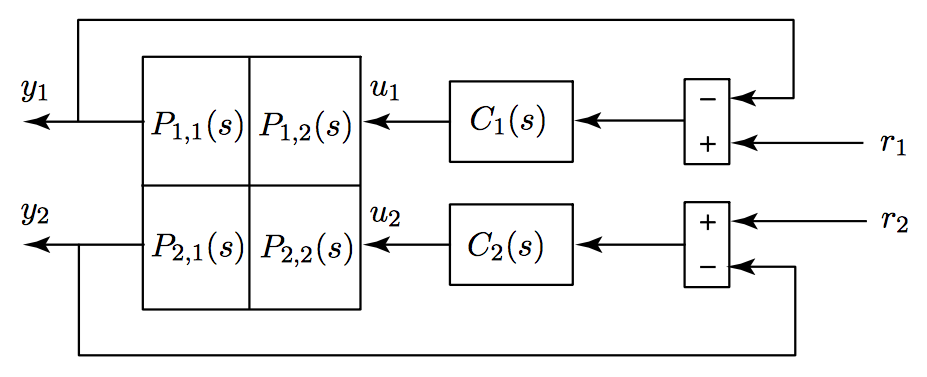
\includegraphics[width=0.7\columnwidth]{rgabsp}
\caption{Structure of MIMO system.}
\label{fig:rgabsp}
\end{center}
\end{figure}
\newpage

\begin{lsg}
\
\begin{enumerate}[(a)]
\item To check if the suggestion is correct let's have a look at the RGA matrix: it holds
\begin{equation*}
\begin{split}
[\text{RGA}]_{11}&=[\text{RGA}]_{22}\\
&=\frac{P_{11}(s)\cdot P_{22}(s)}{P_{11}(s)\cdot P_{22}(s)-P_{12}(s)\cdot P_{21}(s)}\\
&=1.\\
[\text{RGA}]_{12}&=[\text{RGA}]_{21}\\
&=1-[\text{RGA}]_{11}\\
&=0.
\end{split}
\end{equation*}
since $P_{12}(s)=0$. This means that the RGA matrix is identical to the identity matrix, resulting in a perfect diagonal dominant system, which can be controlled with the \textit{one loop at the time} approach.
\item Let's analyze the signals from Figure \ref{fig:rgabsp}. Since $P_{12}(s)=0$, the output $y_1$ is not affected from $u_2$. Moreover, this means that the reference signal $r_2$, which influences $u_2$, cannot affect the output $y_1$. The only reference that acts on both $y_1$ and $y_2$ is $r_1$: directly through $C_1(s)$ on $y_1$ and with crosscouplings through $P_{21}(s)$ on $y_2$.
\item As usual we set to 0 the reference values we don't analyze: here $r_2=0$. Starting from the general equation in frequency domain 
\begin{equation*}
\begin{split}
\begin{pmatrix}
Y_1(s)\\
Y_2(s)
\end{pmatrix}&=\begin{pmatrix}
P_{11}(s)&P_{12}(s)\\
P_{21}(s)&P_{22}(s)
\end{pmatrix}\cdot 
\begin{pmatrix}
U_1(s)\\
U_2(s)
\end{pmatrix}\\
&=\begin{pmatrix}
P_{11}(s)&0\\
P_{21}(s)&P_{22}(s)
\end{pmatrix}\cdot 
\begin{pmatrix}
U_1(s)\\
U_2(s)
\end{pmatrix}.
\end{split}
\end{equation*}
one can read
\begin{equation*}
\begin{split}
Y_1(s)&=P_{11}(s)\cdot U_1(s)\\
Y_2(s)&=P_{21}(s)\cdot U_1(s)+P_{22}(s)\cdot U_2(s).
\end{split}
\end{equation*}
Since we want to relate $r_1$ and $y_2$ let's express $u_1$ as something we know. \\ Using Figure \ref{fig:rgabsp} one gets
\begin{equation*}
\begin{split}
R_1(s)\cdot C_1(s)&=U_1(s)+P_{11}(s)\cdot C_1(s)\cdot U_1(s)\\
U_1&=\frac{R_1(s)\cdot C_1(s)}{1+P_{11}(s)\cdot C_1(s)}.
\end{split}
\end{equation*}
Inserting this into the second equation one gets
\begin{equation*}
Y_2(s)=P_{21}(s)\cdot \frac{R_1(s)\cdot C_1(s)}{1+P_{11}(s)\cdot C_1(s)}+P_{22}(s)\cdot U_2(s).
\end{equation*}
One have to find an expression for $U_2(s)$. To do that, we look at the second loop in Figure \ref{fig:rgabsp} an see
\begin{equation*}
\begin{split}
\underbrace{R_2(s)}_{=0}\cdot C_2(s)-Y_2(s)\cdot C_2(s)&=U_2(s)\\
U_2(s)&=-Y_2(s)\cdot C_2(s).
\end{split}
\end{equation*}
Inserting this into the second equation one gets
\begin{equation*}
\begin{split}
Y_2(s)&=P_{21}(s)\cdot \frac{R_1(s)\cdot C_1(s)}{1+P_{11}(s)\cdot C_1(s)}+P_{22}(s)\cdot U_2(s)\\
&=P_{21}(s)\cdot \frac{R_1(s)\cdot C_1(s)}{1+P_{11}(s)\cdot C_1(s)}+P_{22}(s)\cdot (-Y_2(s)\cdot C_2(s))\\
Y_2(s)\cdot (1+P_{22}(s)\cdot C_2(s))&=P_{21}(s)\cdot \frac{R_1(s)\cdot C_1(s)}{1+P_{11}(s)\cdot C_1(s)}\\
Y_2(s)&=\underbrace{\frac{P_{21}(s)\cdot C_1(s)}{(1+P_{11}(s)\cdot C_1(s))\cdot(1+P_{22}(s)\cdot C_2(s))}}_{F(s)}\cdot R_1(s).
\end{split}
\end{equation*}
where $F(s)$ is the transfer function we wanted.


\end{enumerate}

\end{lsg}

\end{bsp}

\newpage
\begin{bsp}
Figure \ref{fig:rgatransf} shows the structure of a MIMO system, composed of three subsystems $P_1(s),P_2(s)$ and $P_3(s)$. It has inputs $u_1$ and $u_2$ and outputs $y_1$ and $y_2$.
\begin{figure}[ht]
\begin{center}
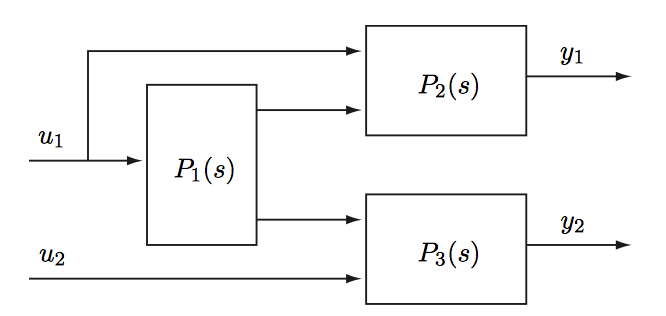
\includegraphics[width=0.65\columnwidth]{rgatransf}
\caption{Structure of MIMO system.}
\label{fig:rgatransf}
\end{center}
\end{figure}
The three subsystems are given as
\begin{equation*}
P_1(s)=\begin{pmatrix}
\frac{s-5}{s+3}\\[6pt]
\frac{1}{s+4}
\end{pmatrix}, \ \ P_2(s)=\begin{pmatrix}
\frac{1}{s+3}&\frac{s+4}{s-5}
\end{pmatrix}, \ \ P_3(s)=\begin{pmatrix} \frac{s+2}{s+5}&\frac{1}{s+1} \end{pmatrix}.
\end{equation*}
Compute the transfer function of the whole system.

\newpage
\begin{lsg}
One should think with matrix dimensions here. Let's redefine the subsystem's matrices more generally:
\begin{equation*}
P_1(s)=\begin{pmatrix}
P_1^{11}\\
P_1^{21}\\
\end{pmatrix}, \ \ P_2(s)=\begin{pmatrix}
P_2^{11}&P_2^{12}
\end{pmatrix}, \ \ P_3(s)=\begin{pmatrix} P_3^{11}&P_3^{12} \end{pmatrix}
\end{equation*}
Together with the structure of the system one gets
\begin{equation*}
\begin{split}
Y_1&=P_2^{11}\cdot U_1+P_2^{12}\cdot P_1^{11}\cdot U_1,\\
Y_2&=P_3^{11}\cdot P_1^{21}\cdot U_1+P_3^{12}\cdot U_2.
\end{split}
\end{equation*}
This can be written in the general matrix for the transfer function:
\begin{equation*}
\begin{split}
P(s)&=\begin{pmatrix}
P_2^{11}+P_2^{12}\cdot P_1^{11}&0 \\
P_3^{11}\cdot P_1^{21}&P_3^{12}
\end{pmatrix}\\
&=\begin{pmatrix}
\frac{1}{s+3}+\frac{s+4}{s-5}\cdot \frac{s-5}{s+3}&0 \\[6pt]
\frac{s+2}{s+5}\cdot \frac{1}{s+4}&\frac{1}{s+1}
\end{pmatrix}\\
&=\begin{pmatrix}
\frac{s+5}{s+3}&0\\[6pt]
\frac{s+2}{(s+5)\cdot (s+4)}&\frac{1}{s+1}
\end{pmatrix}.
\end{split}
\end{equation*}

\end{lsg}

\end{bsp}


\newpage
\begin{bsp}
Figure \ref{fig:rgatransfers} shows the structure of a MIMO system, composed of two subsystems $P_1(s),P_2(s)$. It has inputs $u_1$ and $u_2$ and outputs $y_1$ and $y_2$.
\begin{figure}[ht]
\begin{center}
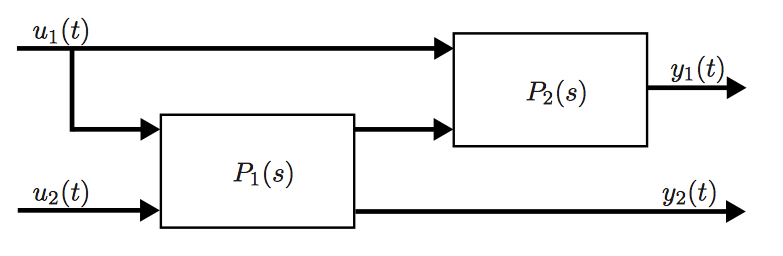
\includegraphics[width=0.65\columnwidth]{rgatransfers}
\caption{Structure of MIMO system.}
\label{fig:rgatransfers}
\end{center}
\end{figure}
The subsystem $P_1(s)$ is given with its state space description:
\begin{equation*}
A_1=\begin{pmatrix}
-3&0\\
2&1
\end{pmatrix}, \ \ B_1=\begin{pmatrix}
1&0\\
2&1
\end{pmatrix}, \ \ C_1=\begin{pmatrix}
0&2\\
3&1
\end{pmatrix}\ \ 
D_1=\begin{pmatrix}
0&1\\
0&0
\end{pmatrix}.
\end{equation*}
and the subsystem $P_2(s)$ is given as
\begin{equation*}
P_2(s)=\begin{pmatrix}
\frac{1}{s-2}&\frac{s-1}{(s+4)\cdot (s-2)}
\end{pmatrix}.
\end{equation*}
Compute the transfer function of the whole system.
\newpage

\begin{lsg}
First of all, we compute the transfer function in frequency domain of the first subsystem $P_1(s)$. It holds
\begin{equation*}
\begin{split}
P_1(s)&=C_1\cdot (s\cdot \mathbb{1}-A_1)^{-1}\cdot B_1 + D_1\\
&=\begin{pmatrix}
0&2\\
3&1
\end{pmatrix}\cdot 
\begin{pmatrix}
s+3&0\\
-2&s-1
\end{pmatrix}^{-1}\cdot \begin{pmatrix}
1&0\\
2&1
\end{pmatrix}+\begin{pmatrix}
0&1\\
0&0
\end{pmatrix}\\
&= \begin{pmatrix}
0&2\\
3&1
\end{pmatrix}\cdot 
\frac{1}{(s+3)\cdot (s-1)}\cdot
\begin{pmatrix}
s-1&0\\
2&s+3
\end{pmatrix}\cdot \begin{pmatrix}
1&0\\
2&1
\end{pmatrix}+\begin{pmatrix}
0&1\\
0&0
\end{pmatrix}\\
&=\frac{1}{(s+3)\cdot (s-1)} \cdot \begin{pmatrix}
0&2\\
3&1
\end{pmatrix}\cdot \begin{pmatrix}
 s-1&0\\
2s+8&s+3
 \end{pmatrix}+\begin{pmatrix}
0&1\\
0&0
\end{pmatrix}\\
&=\frac{1}{(s+3)\cdot (s-1)}\cdot \begin{pmatrix}
 4s+16&2s+6\\
 5s+5&s+3
 \end{pmatrix}\\
 &=\begin{pmatrix}
\frac{4s+16}{(s+3)\cdot (s-1)}&\frac{2}{s-1}\\[6pt]
\frac{5s+5}{(s+3)\cdot (s-1)}&\frac{1}{s-1}
\end{pmatrix}.
\end{split}
\end{equation*}
One should think with matrix dimensions here. Let's redefine the subsystem's matrices more generally:
\begin{equation*}
P_1(s)=\begin{pmatrix}
P_1^{11}&P_1^{12}\\
P_1^{21}&P_1^{22}\\
\end{pmatrix}, \ \ P_2(s)=\begin{pmatrix}
P_2^{11}&P_2^{12}
\end{pmatrix}.
\end{equation*}
Together with the structure of the system one gets
\begin{equation*}
\begin{split}
Y_1&=P_2^{11}\cdot U_1+P_1^{11}\cdot P_2^{12}\cdot U_1+P_1^{12}\cdot P_2^{12}\cdot U_2,\\
Y_2&=P_1^{21}\cdot U_1 +P_1^{22}\cdot U_2.
\end{split}
\end{equation*}
This can be written in the general matrix for the transfer function:
\begin{equation*}
\begin{split}
P(s)&=\begin{pmatrix}
P_2^{11}+P_1^{11}\cdot P_2^{12}&P_1^{12}\cdot P_2^{12} \\
P_1^{21}& P_1^{22}
\end{pmatrix}\\
&=\hdots \\
&= \begin{pmatrix}
 \frac{s+7}{(s+3)\cdot (s-2)}&\frac{s+1}{(s+4)(s-2)}\\[6pt]
 \frac{5s+5}{(s+3)\cdot (s-1)}&\frac{1}{s-1}
 \end{pmatrix}.
\end{split}
\end{equation*}

\end{lsg}




\end{bsp}
\newpage

\begin{bsp}
The system in Figure \ref{fig:mcrga} can be well controlled with two separate SISO controllers.
\begin{figure}[ht]
\begin{center}
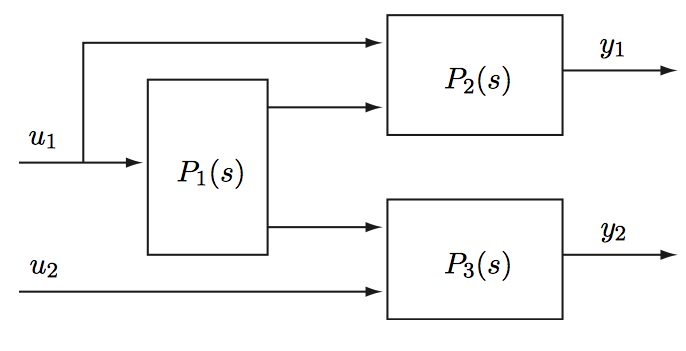
\includegraphics[width=0.65\columnwidth]{mcrga}
\caption{Structure of MIMO system.}
\label{fig:mcrga}
\end{center}
\end{figure}

\begin{todolist}
 \item True.
 \item False.
\end{todolist}
\newpage
\begin{lsg}
\ 
\begin{todolist}
 \item [\done] True.
 \item False.
\end{todolist}
\subsubsection*{Explanation:}
One can observe that the input $u_2$ affects only the output $y_2$. This means that the transfer function matrix has a \textbf{triangular} form and hence, that the RGA matrix is identical to the identity matrix: this means that we can reach good control with two separate SISO controllers.


\end{lsg}


\end{bsp}



\newpage
\section{Frequency Response of MIMO Systems}
\subsection{Singular Value Decomposition (SVD)}
The Singular Value Decomposition plays a central role in MIMO frequency response analysis. Let's recall some concepts from the course \textit{Lineare Algebra I/II}:
\subsubsection{Preliminary Definitions}
The \textbf{induced} norm $||A||$ of a matrix that describes a linear function like
\begin{equation}
y=A\cdot u
\label{eq:lin}
\end{equation}
is defined as
\begin{equation}
\begin{split}
||A||&=\max_{u\neq 0}\frac{||y||}{||u||}\\
&=\max_{||u||=1}||y||.
\end{split}
\label{eq:gen}
\end{equation}
\begin{bmk}
\
In the course \textit{Lineare Algebra I/II} you learned that there are many different norms and the expression $||A||$ could look too generic. However, in this course we will always use the euclidean norm $||A||=||A||_2$.
This norm is defined as
\begin{equation}
\begin{split}
||A||_2&=\sqrt{\mu_{max}}\\
&=\sqrt{\text{maximal eigenvalue of }A^*\cdot A}
\end{split}
\end{equation}
where $A^*$ is the \textbf{conjugate transpose} or \textbf{Hermitian transpose} of the matrix $A$. This is defined as
\begin{equation}
A^*=(conj(A))^T.
\end{equation}
\end{bmk}
\begin{bsp}
Let 
\begin{equation*}
A=\begin{pmatrix}
1&-2-i\\
1+i&i
\end{pmatrix}.
\end{equation*}
Then it holds
\begin{equation*}
\begin{split}
A^*&=(conj(A))^T\\
&=
\begin{pmatrix}
1&-2+i\\
1-i&-i
\end{pmatrix}^T\\
&=\begin{pmatrix}
1&1-i\\
-2+i&-i
\end{pmatrix}.
\end{split}
\end{equation*}
\end{bsp}
\begin{bmk}
If we deal with $A\in \mathbb{R}^{n\times m}$ holds of course
\end{bmk}
\begin{equation}
A^*=A^T.
\end{equation}
One can list a few useful properties of the euclidean norm:
\begin{enumerate}[(i)]
\item Remember: $A^T\cdot A$ is always a quadratic matrix!
\item If $A$ is orthogonal:
\begin{equation}
||A||_2=1.
\end{equation}
\item If $A$ is symmetric:
\begin{equation}
||A||_2=\max(|e_i|).
\end{equation}
\item If $A$ is invertible:
\begin{equation}
\begin{split}
||A^{-1}||_2&=\frac{1}{\sqrt{\mu_{min}}}\\
&=\frac{1}{\sqrt{\text{minimal eigenvalue of }A^*\cdot A}}.
\end{split}
\end{equation}
\item If $A$ is invertible and symmetric:
\begin{equation}
||A^{-1}||_2=\frac{1}{\min(|e_i|)}.
\end{equation}
\end{enumerate}
where $e_i$ are the eigenvalues of $A$. \\
In order to define the SVD we have to go a step further. Let's consider a Matrix $A$ and the linear function \ref{eq:lin}. It holds
\begin{equation}
\begin{split}
||A||^2&=\max_{||u||=1}y^*\cdot y\\
&=\max_{||u||=1} (A\cdot u)^*\cdot (A\cdot u)\\
&=\max_{||u||=1}u^*\cdot A^*\cdot A\cdot u\\
&=\max_i \mu(A^*\cdot A)\\
&= \max_i \sigma_i^2.
\end{split}
\end{equation}
where $\sigma_i$ are the \textbf{singular values} of matrix $A$. They are defined as
\begin{equation}
\sigma_i=\sqrt{\mu_i}
\label{eq:sv}
\end{equation}
where $\mu_i$ are the eigenvalues of $A^*\cdot A$. \\
Combining \ref{eq:gen} and \ref{eq:sv} one gets
\begin{equation}
\sigma_{min}(A)\leq \frac{||y||}{||u||}\leq \sigma_{max}(A).
\end{equation}

\begin{figure}[ht]
\begin{center}
\begin{tikzpicture}[scale=1.5]
\draw[->, thick] (-2, 0) -- (2, 0);
\draw[->, thick] (0, -2) -- (0, 2);
\draw[dashed] (0,0) circle (1);
\draw[->, thick] (0,0) -- (35:1) node [above right]{$u$};
\draw[black!35!blue,rotate = 35] (0,0) ellipse (2 and .7);
\draw[black!35!blue, ->, thick, rotate = 35] (0,0) -- (90:.7) node [left]{\footnotesize{$y = M\cdot u$}};
\end{tikzpicture}
\end{center}
\caption{Illustration of the singular values.}
\end{figure}

\subsubsection{Singular Value Decomposition}

Our goal is to write a general matrix  $A \in \mathbb{C}^{p \times m}$ as product of three matrices: $U$, $\Sigma $ and $V$. It holds

\begin{equation}
A=U\cdot \Sigma \cdot V^* \ \text{with } U \in \mathbb{C}^{p\times p},\ \Sigma \in \mathbb{R}^{p\times m},\ V\in \mathbb{C}^{m\times m}.
\end{equation}

\begin{bmk}
$U$ and $V$ are orthogonal, $\Sigma $ is a diagonal matrix.
\end{bmk}
\newpage
\subsubsection*{Kochrezept:}
Let  $A \in \mathbb{C}^{p\times m}$ be given:
\begin{enumerate}[(I)]
\item Compute all the eigenvalues and eigenvectors of the matrix 
$$A^*\cdot A  \in \mathbb{C}^{m\times m}.$$
and sort them as
\begin{equation}
\mu_1\geq \mu_2\geq \hdots \geq \mu_r>\mu_{r+1}=\hdots=\mu_m=0
\end{equation}
\item Compute an orthogonal basis from the eigenvectors $v_i$ and write it in a matrix as
\begin{equation}
V=(v_1\ \hdots \ v_m) \in \mathbb{C}^{m\times m}.
\end{equation}
\item We have already found the singular values: they are defined as
\begin{equation}
\sigma_i=\sqrt{\mu_i}
\text{ for } i=1,\hdots,\min\{p,m\}.
\end{equation}
We can then write $\Sigma $ as
\begin{equation}
\Sigma=\begin{pmatrix}
\sigma_1&&&0&\hdots&0 \\
&\ddots&&\vdots&&\vdots \\
&&\sigma_m&0&\hdots&0 \\
\end{pmatrix}\ \in \mathbb{R}^{p\times m},\ p<m
\end{equation}
\begin{equation}
\Sigma=\begin{pmatrix}
\sigma_1&&\\
&\ddots&\\
&&\sigma_n\\
0&\hdots&0\\
\vdots&&\vdots\\
0&\hdots&0\\
\end{pmatrix} \in \mathbb{R}^{p\times m},\ p>m.
\end{equation}
\item One finds $u_1,\hdots,u_r$ from \begin{equation}
u_i={1\over \sigma_i}\cdot A\cdot v_i \text{ for all } i=1,\hdots,r \text{ (for } \sigma_i\neq0)
\end{equation}
\item If $r<p$ one has to complete the basis  $u_1,\hdots,u_r$ (with ONB) to obtain an orthogonal basis, with $U$ orthogonal.
\item If you followed the previous steps, you can write
$$A=U\cdot \Sigma \cdot V^*.$$
\end{enumerate}
\textbf{Motivation for the computation of $\Sigma$, $U$ und $V$}.
\begin{equation}
\begin{split}
A^\ast\cdot A&=(U\cdot\Sigma\cdot V^\ast)^\ast\cdot(U\cdot\Sigma\cdot V^\ast)\\
&=V\cdot\Sigma^\ast\cdot U^\ast\cdot U\cdot\Sigma\cdot V^\ast\\
&=V\cdot\Sigma^\ast\cdot\Sigma\cdot V^\ast\\
&=V\cdot\Sigma^2\cdot V^\ast.
\end{split}
\end{equation}
This is nothing else than the \textbf{diagonalization} of the matrix $A^\ast\cdot A$. The columns of $V$ are the eigenvectors of $A^\ast\cdot A$ and the $\sigma_i^2$ the eigenvalues. \\ 
For $U$:
\begin{equation}
\begin{split}
A\cdot A^\ast &=(U\cdot\Sigma\cdot V^\ast)\cdot(U\cdot\Sigma\cdot V^\ast)^\ast\\
&=U\cdot\Sigma\cdot V^\ast\cdot V\cdot\Sigma\cdot U^\ast\\
&=U\cdot\Sigma^\ast\cdot\Sigma\cdot U^\ast\\
&=U\cdot\Sigma^2\cdot U^\ast.
\end{split}
\end{equation}
This is nothing else than the \textbf{diagonalization} of the matrix $A\cdot A^\ast$. The columns of $U$ are the eigenvectors of $A\cdot A^\ast$ and the $\sigma_i^2$ the eigenvalues. \\ 
\begin{bmk}
In order to derive the previous two equations I used that:
\begin{itemize}
\item The matrix $A^\ast\cdot A$ is symmetric, i.e.
\begin{equation*}
\begin{split}
(A^\ast\cdot A)^\ast &=A^\ast\cdot (A^\ast)^\ast\\
&=A^\ast \cdot A.
\end{split}
\end{equation*}
\item $U^{-1}=U^\ast$ (because $U$ is othogonal).
\item $V^{-1}=V^\ast$ (because $V$ is othogonal).
\end{itemize}
\end{bmk}
\begin{bmk}
Since the matrix $A^\ast\cdot A$ is always  symmetric and positive semidefinite, the singular values are always real numbers. 
\end{bmk}

\begin{bmk}
The \textsc{Matlab} command for the singular value decomposition is
\begin{verbatim}
[U,S,V]=svd
\end{verbatim}
One can write $A^T$ as \verb+ A.'=transpose(A)+ and $A^*$ as \verb+A'=conj(transpose(A))+. Those two are equivalent for real numbers.
\end{bmk}
\begin{bmk}
Although I've reported detailed informations about the calculation of $U$ and $V$, this \textbf{won't be relevant for the exam}. It is however good and useful to know the reasons that are behind this topic.
\end{bmk}

\newpage
\begin{bsp}
Let $u$ be
\begin{equation*}
u=\begin{pmatrix}
\cos(x)\\
\sin(x)
\end{pmatrix}
\end{equation*}
with $||u||=1$. The matrix $M$ is given as
\begin{equation*}
M=\begin{pmatrix}
2&0\\[6pt]
0&{1\over2}\\
\end{pmatrix}.
\end{equation*}
We know that the product of $M$ and $u$ defines a linear function
\begin{equation*}
\begin{split}
y&=M\cdot u\\
&=\begin{pmatrix}
2&0\\[6pt]
0&{1\over2}\\
\end{pmatrix}\cdot \begin{pmatrix}
\cos(x)\\
\sin(x)
\end{pmatrix}\\
&=\begin{pmatrix}
2\cdot \cos(x)\\[6pt]
\frac{1}{2} \cdot \sin(x) 
\end{pmatrix}.
\end{split}
\end{equation*}
We need the maximum of $||y||$. In order to avoid square roots, one can use that the $x$ that maximizes $||y||$ should also maximize $||y||^2$.
\begin{equation*}\label{maxbet}
\Vert y \Vert^2 = 4\cdot\cos^2(x)+\frac{1}{4}\cdot\sin^2(x)
\end{equation*}
has maximum
\begin{equation*}
\begin{split}
\frac{\text{d}|| y ||^2}{\text{d}x}&=-8\cdot\cos(x)\cdot\sin(x)+\frac{1}{2}\cdot\sin(x)\cdot\cos(x)\overset{!}{=}0\\
&\Rightarrow\quad x_\text{max}=\left\{0,\frac{\pi}{2},\pi,\frac{3\pi}{2}\right\}.
\end{split}
\end{equation*}
Inserting back for the maximal $||y||$ one gets:
\begin{equation*}
|| y||_\text{max}=2, \qquad  || y||_\text{max}=\frac{1}{2}.
\end{equation*}
The singular values can be calculated with $M^*\cdot M$:
\begin{equation*}
\begin{split}
M^\ast\cdot M&=M^\intercal\cdot M\\
&=\begin{pmatrix} 4 & 0 \\ 0 & \frac{1}{4} \end{pmatrix} \quad \Rightarrow\quad \lambda_i=\left\{4,\frac{1}{4}\right\} \quad \Rightarrow\quad \sigma_i=\left\{2,\frac{1}{2}\right\}.
\end{split}
\end{equation*}
As stated before, one can see that $|| y|| \in[\sigma_\text{min},\sigma_\text{max}]$.
The matrix $U$ has eigenvectors of $M\cdot M^\intercal$ as coulmns and the matrix $V$ has eigenvectors of $M^\intercal\cdot M$ as columns. \\
In this case $$M\cdot M^\intercal=M^\intercal\cdot M,$$ hence the two matrices are equal. Since their product is a diagonal matrix one should recall from the theory that the eigenvectors are easy to determine: they are nothing else than the standard basis vectors. This means
\begin{equation*}
U = \begin{bmatrix} 1 & 0 \\ 0 & 1\end{bmatrix}, \qquad \Sigma=\begin{bmatrix} 2 & 0 \\ 0 & \frac{1}{2}\end{bmatrix}, \qquad V=\begin{bmatrix} 1 & 0 \\ 0 & 1\end{bmatrix}.
\end{equation*}
\subsubsection*{Interpretation:}
Referring to Figure \ref{fig:svdex}, let's interprete these calculations. One can see that the maximal \textit{amplification} occurs at $v=V(:,1)$ and has direction $u=U(:,1)$, i.e. the vector $u$ is doubled ($\sigma_{max}$). The minimal \textit{amplification} occurs at $v=V(:,2)$ and has direction $u=U(:,2)$, i.e. the vector $u$ is halved ($\sigma_{min}$)

\begin{figure}[ht]
\begin{center}
\begin{tikzpicture}[scale=1.5]
\draw[->, thick] (-2.5, 0) -- (2.5, 0);
\draw[->, thick] (0, -2) -- (0, 2);
\draw[dashed] (0,0) circle (1);
\draw[black!35!blue] (0,0) ellipse (2 and 0.5);
\draw[->, thick] (0,0) -- (45:1) node [right]{$u$};
\draw[black!35!blue, ->, thick] (0,0) -- (14:1.45) node [above right] {$y = M\cdot u$};
\node[below right] at (2,0) {2};
\node[below right] at (1,0) {1};
\node[above left] at (0, 1) {1};
\node[above left] at (0, 0.5) {0.5};
\end{tikzpicture}
\end{center}
\caption{Illustration von der Singularwertzerlegung.}
\label{fig:svdex}
\end{figure}
\end{bsp}

\pagebreak

\begin{bsp}
Let
$$A=\begin{pmatrix}
-3&0\\
0&3\\
\sqrt{3}&2\\
\end{pmatrix}$$
be given.\\
\textbf{Question:} Find the singular values of $A$ and write down the matrix $\Sigma$.
\begin{lsg}
Let's compute $A^TA$:
$$A^TA=\begin{pmatrix}
-3&0&\sqrt{3}\\
0&3&2\\
\end{pmatrix}\cdot \begin{pmatrix}
-3&0\\
0&3\\
\sqrt{3}&2\\
\end{pmatrix}=\begin{pmatrix}
12&2\sqrt{3}\\
2\sqrt{3}&13\\
\end{pmatrix}$$
One can see easily that the eigenvalues are
$$\lambda_1=16,\ \lambda_2=9.$$
The singular values are
$$\sigma_1=4,\ \sigma_2=3.$$
One writes in this case$$\Sigma=\begin{pmatrix}
4&0\\
0&3\\
0&0\\
\end{pmatrix}.$$
\end{lsg}
\end{bsp}

\newpage
\begin{bsp}
A transfer function $G(s)$ is given as
\begin{equation*}
\begin{pmatrix}
\frac{1}{s+3}&\frac{s+1}{s+3}\\[6pt]
\frac{s+1}{s+3}&\frac{1}{s+3}
\end{pmatrix}
\end{equation*}
Find the singular values of $G(s)$ at $\omega=1 \frac{\text{rad}}{s}$.
\newpage

\begin{lsg}
The transfer function $G(s)$ evaluated at $\omega=1\frac{\text{rad}}{{s}}$ has the form
\begin{equation*}
G(j)=\begin{pmatrix}
\frac{1}{j+3}&\frac{j+1}{j+3}\\[6pt]
\frac{j+1}{j+3}&\frac{1}{j+3}
\end{pmatrix}
\end{equation*}
In order to calculate the singular values, we have to compute the eigenvalues of $H=G^*\cdot G$:
\begin{equation*}
\begin{split}
H&=G^*\cdot G\\
&=\begin{pmatrix}
\frac{1}{-j+3}&\frac{-j+1}{-j+3}\\[6pt]
\frac{-j+1}{-j+3}&\frac{1}{-j+3}
\end{pmatrix}\cdot \begin{pmatrix}
\frac{1}{j+3}&\frac{j+1}{j+3}\\[6pt]
\frac{j+1}{j+3}&\frac{1}{j+3}
\end{pmatrix}\\
&=\begin{pmatrix}
\frac{3}{10}&\frac{2}{10}\\[6pt]
\frac{2}{10}&\frac{3}{10}
\end{pmatrix}\\
&=\frac{1}{10}\cdot \begin{pmatrix}
3&2\\
2&3
\end{pmatrix}.
\end{split}
\end{equation*}
For the eigenvalues it holds
\begin{equation*}
\begin{split}
\det(H-\lambda \cdot \mathbb{1})&=\det \begin{pmatrix}
\frac{3}{10}-\lambda&\frac{2}{10}\\[6pt]
\frac{2}{10}&\frac{3}{10}-\lambda
\end{pmatrix}\\
&=\left(\frac{3}{10}-\lambda \right)^2-\left(-\frac{2}{10}\right)^2\\
&=\lambda^2-\frac{6}{10}\lambda +\frac{5}{100}\\
&=\left(\lambda -\frac{1}{10} \right)\cdot \left(\lambda -\frac{5}{10} \right).
\end{split}
\end{equation*}
It follows
\begin{equation*}
\begin{split}
\lambda_1 &= \frac{1}{10}\\
\lambda_2 &= \frac{1}{2}
\end{split}
\end{equation*}
and so
\begin{equation*}
\begin{split}
\sigma_1 &=\sqrt{ \frac{1}{10}}\\
&\approx 0.3162.\\
\sigma_2 &= \sqrt{\frac{1}{2}}\\
&\approx 0.7071.
\end{split}
\end{equation*}


\end{lsg}
\end{bsp}

\newpage

\begin{bsp}
Let be
\begin{equation*}
\begin{split}
A&=\begin{pmatrix}
1&2\\
0&1
\end{pmatrix}\\
B&=\begin{pmatrix}
j&1
\end{pmatrix}.
\end{split}
\end{equation*}
Find the singular values of the two matrices.
\newpage
\begin{lsg}
\
\begin{itemize}
\item Let's begin with matrix $A$. It holds
\end{itemize}
\begin{equation*}
\begin{split}
H&=A^*\cdot A\\
&=\begin{pmatrix}
1&0\\
2&1
\end{pmatrix}\cdot \begin{pmatrix}
1&2\\
0&1
\end{pmatrix}\\
&=\begin{pmatrix}
1&2\\
2&5
\end{pmatrix}.
\end{split}
\end{equation*}
In order to find the eigenvalues of $H$ we compute
\begin{equation*}
\begin{split}
\det(H-\lambda \cdot \mathbb{1})&=\det \begin{pmatrix}
 1-\lambda &2\\
2&5-\lambda
\end{pmatrix}\\
&=(1-\lambda)\cdot (5-\lambda)-4\\
&=\lambda^2-6\lambda +1.
\end{split}
\end{equation*}
This means that the eigenvalues are
\begin{equation*}
\begin{split}
\lambda_1 &=3+ 2\sqrt{2}\\
\lambda_2 &=3- 2\sqrt{2}.
\end{split}
\end{equation*}
The singular values are then
\begin{equation*}
\begin{split}
\sigma_1 &\approx 2.4142\\
\sigma_2 &\approx  0.4142.
\end{split}
\end{equation*}
\begin{itemize}
\item Let's look at matrix $B$. It holds
\end{itemize}
\begin{equation*}
\begin{split}
F&=B^*\cdot B\\
&=\begin{pmatrix}
-j\\
1
\end{pmatrix}\cdot \begin{pmatrix}
 j&1
 \end{pmatrix}\\
 &=\begin{pmatrix}
1&-j\\
j&1
\end{pmatrix}.
\end{split}
\end{equation*}
In order to find the eigenvalues of $F$ we compute
\begin{equation*}
\begin{split}
\det(F-\lambda \cdot \mathbb{1})&=\det \begin{pmatrix}
 1-\lambda &-j\\
j&1-\lambda
\end{pmatrix}\\
&=(1-\lambda)^2-1\\
&=\lambda^2-2\lambda\\
&=\lambda \cdot (\lambda -2).
\end{split}
\end{equation*}
This means that the eigenvalues are
\begin{equation*}
\begin{split}
\lambda_1 &=0\\
\lambda_2 &=2.
\end{split}
\end{equation*}
The singular values are then
\begin{equation*}
\begin{split}
\sigma_1 &= 0\\
\sigma_2 &=  \sqrt{2}.
\end{split}
\end{equation*}
\end{lsg}

\end{bsp}
\newpage
\subsection{Frequency Responses}
As we learned for SISO systems, if one excites a system with an \textit{harmonic} signal
\begin{equation}
u(t)=h(t)\cdot \cos(\omega \cdot t),
\end{equation}
the answer after a big amount of time is still an harmonic function with equal frequency $\omega$:
\begin{equation}
y_{\infty}(t)=|P(j\cdot \omega)| \cos(\omega \cdot t+\angle(P(j\cdot \omega))).
\end{equation}
One can generalize this and apply it to MIMO systems. With the assumption of $p=m$, i.e. equal number of inputs and outputs, one excite a system with
\begin{equation}
u(t)=\begin{pmatrix}
\mu_1\cdot \cos (\omega \cdot t + \phi_1)\\
\vdots\\
\mu_m\cdot \cos (\omega \cdot t + \phi_m)\\
\end{pmatrix}\cdot h(t)
\end{equation}
and get
\begin{equation}
y_{\infty}(t)=\begin{pmatrix}
\nu_1\cdot \cos (\omega \cdot t + \psi_1)\\
\vdots\\
\nu_m\cdot \cos (\omega \cdot t + \psi_m)\\
\end{pmatrix}.
\end{equation}
Let's define two diagonal matrices
\begin{equation}
\begin{split}
\Phi &=\text{diag}(\phi_1,\hdots,\phi_m)\in \mathbb{R}^{m\times m},\\
\Psi &=\text{diag}(\psi_1,\hdots,\psi_m)\in \mathbb{R}^{m\times m}
\end{split}
\end{equation}
and two vectors
\begin{equation}
\begin{split}
\mu &=\begin{pmatrix}
\mu_1 &\hdots &\mu_m
\end{pmatrix}^T,  \\
\nu &=\begin{pmatrix}
\nu_1 &\hdots &\nu_m
\end{pmatrix}^T.
\end{split}
\end{equation}
With these one can compute the Laplace Transform of the two signals as:
\begin{equation}
U(s)=e^{\frac{\Phi \cdot s}{\omega}}\cdot \mu \cdot \frac{s}{s^2+\omega^2}.
\end{equation}
and
\begin{equation}
Y(s)=e^{\frac{\Psi \cdot s}{\omega}}\cdot \nu \cdot \frac{s}{s^2+\omega^2}.
\end{equation}
With the general equation for a systems one gets
\begin{equation}
\begin{split}
Y(s)&=P(s)\cdot U(s)\\
e^{\frac{\Psi \cdot s}{\omega}}\cdot \nu \cdot \frac{s}{s^2+\omega^2}&=P(s)\cdot e^{\frac{\Phi \cdot s}{\omega}}\cdot \mu \cdot \frac{s}{s^2+\omega^2}\\
e^{\frac{\Psi \cdot j \cdot \omega}{\omega}}\cdot \nu &=P(s)\cdot e^{\frac{\Phi \cdot j\cdot \omega}{\omega}}\cdot \mu\\
e^{\Psi \cdot j}\cdot \nu &=P(s)\cdot e^{\Phi \cdot j}\cdot \mu.
\end{split}
\end{equation}
We then recall that the \textbf{induced norm} for the matrix of a linear transformation $y=A\cdot u$ from \ref{eq:gen}. Here it holds
\begin{equation}
\begin{split}
||P(j\cdot \omega)||&=\max_{e^{\Phi \cdot j}\cdot \mu \neq 0}\frac{||e^{\Psi \cdot j}\cdot \nu||}{||e^{\Phi \cdot j}\cdot \mu||}\\
&=\max_{||e^{\Phi \cdot j}\cdot \mu|| =1}||e^{\Psi \cdot j}\cdot \nu||.
\end{split}
\end{equation}
Since
\begin{equation}
||e^{\Phi \cdot j}\cdot \mu||=||\mu||
\end{equation}
and
\begin{equation}
||e^{\Psi \cdot j}\cdot \nu||=||\nu||.
\end{equation}
One gets
\begin{equation}
\begin{split}
||P(j\cdot \omega)||&=\max_{\mu \neq 0}\frac{ ||\nu||}{||\mu||}\\
&=\max_{||\mu||=1}||\nu||.\end{split}
\end{equation}
Here one should get the feeling of why we introduced the singular value decomposition. From the theory we've learned, it is clear that
\begin{equation}
\sigma_{min}(P(j\cdot \omega))\leq ||\nu||\leq \sigma_{max}(P(j\cdot \omega)).
\end{equation}
and if $||\mu|| \neq 1$
\begin{equation}
\sigma_{min}(P(j\cdot \omega))\leq \frac{||\nu||}{||\mu||}\leq \sigma_{max}(P(j\cdot \omega)).
\end{equation}
with $\sigma_i$ singular values of $P(j\cdot \omega)$.  These two are worst case ranges and is important to notice that there is no exact formula for $\nu=f(\mu)$.
\subsubsection{Maximal and minimal Gain}
You are given a singular value decomposition 
\begin{equation}
P(j\cdot \omega)=U\cdot \Sigma \cdot V^*.
\end{equation}
One can read out from this decomposition several informations: the maximal/minial gain will be reached with an excitation in the direction of the column vectors of $V$. The response of the system will then be in the direction of the coulmn vectors of $U$.\\
Let's look at an example and try to understand how to use these informations:

\begin{bsp}
We consider a system with $m=2$ inputs and $p=3$ outputs. We are given its singular value decomposition at $\omega=5 \frac{\text{rad}}{\text{s}}$:
\begin{equation*}
\begin{split}
\Sigma&=\begin{pmatrix} 0.4167 & 0 \\ 0  & 0.2631 \\ 0 & 0 \end{pmatrix}, \\
V&=\begin{pmatrix} 0.2908 & 0.9568\\ 0.9443 - 0.1542\cdot j & -0.2870 + 0.0469\cdot j\end{pmatrix}, \\
U&= \begin{pmatrix}-0.0496 - 0.1680\cdot j &  0.1767 - 0.6831\cdot j & -0.6621 - 0.1820\cdot j\\ 0.0146 - 0.9159\cdot j &  -0.1059 + 0.3510\cdot j & -0.1624 + 0.0122\cdot j\\ 0.0349 - 0.3593\cdot j &  0.1360 - 0.5910\cdot j & 0.6782 + 0.2048\cdot j \end{pmatrix}.
\end{split}
\end{equation*}
For the singular value $\sigma_\text{max}=0.4167$ the eigenvectors are $V(:,1)$ and $U(:,1)$:
\begin{align*}
V_1&=\begin{pmatrix} 0.2908\\ 0.9443 - 0.1542\cdot j \end{pmatrix}, &  |V_1|&=\begin{pmatrix} 0.2908 \\ 0.9568 \end{pmatrix}, & \angle(V_1)&=\begin{pmatrix}0 \\ -0.1618\end{pmatrix}, \\
U_1&= \begin{pmatrix}-0.0496 - 0.1680\cdot j \\ 0.0146 - 0.9159\cdot j \\ 0.0349 - 0.3593\cdot j \end{pmatrix}, & |U_1|&=\begin{pmatrix} 0.1752 \\ 0.9160 \\ 0.3609\end{pmatrix}, & \angle(U_1)&=\begin{pmatrix}-1.8581 \\ -1.5548 \\ -1.4741 \end{pmatrix}.
\end{align*}
The maximal gain is then reached with
\begin{equation*}
u(t)=\begin{pmatrix} 0.2908\cdot\cos(5\cdot t) \\ 0.9568\cdot\cos(5\cdot t-0.1618) \end{pmatrix}.
\end{equation*}
The response of the system is then
\begin{equation*}
y(t)=\sigma_\text{max}\cdot\begin{pmatrix}
0.1752\cdot\cos(5\cdot t - 1.8581) \\ 0.9160\cdot\cos(5\cdot t - 1.5548) \\ 0.3609\cdot\cos(5\cdot t - 1.4741)
\end{pmatrix}
=0.4167\cdot\begin{pmatrix}
0.1752\cdot\cos(5\cdot t - 1.8581) \\ 0.9160\cdot\cos(5\cdot t - 1.5548) \\ 0.3609\cdot\cos(5\cdot t - 1.4741)
\end{pmatrix}.
\end{equation*}
Since the three signals $y_1(t)$, $y_2(t)$ and $y_3(t)$ are not in phase, the maximal gain will never be reachen. One can show that
\begin{equation*}
\max_t\Vert y(t)\Vert\approx 0.4160<0.4167=\sigma_\text{max}
\end{equation*}
The reason for this difference stays in the phase deviation between  $y_1(t)$, $y_2(t)$ and $y_3(t)$. The same analysis can be computed for $\sigma_\text{min}$.
\end{bsp}
\subsubsection{Robustness and Disturbance Rejection}
Let's redefine the matrix norm $\Vert\cdot\Vert_\infty$ as
\begin{equation}
\Vert G(s)\Vert_\infty = \max\limits_{\omega}(\max\limits_{i}( \sigma_i(G(i\cdot \omega))).
\end{equation}
\begin{bmk}
It holds
\begin{equation}
\Vert G_1(s)\cdot G_2(s)\Vert_\infty \leq \Vert G_1(s)\Vert_\infty \cdot \Vert G_2(s)\Vert_\infty .
\end{equation}
\end{bmk}
As we did for SISO systems, we can resume some important indicators for robustness and noise amplification:

\begin{center}
\begin{tabular}{l|c|c} \toprule
  & SISO & MIMO \\ \midrule
Robustness & $\mu = \min\limits_{\omega} \left( |1+L(j \cdot \omega)| \right) $ & $\mu = \min\limits_{\omega} \left(\sigma_{\text{min}} (\mathbb{I} + L(j\cdot \omega)) \right)$ \\ \midrule
Noise Amplification & $||S||_\infty = \max\limits_{\omega} \left(|S(j \cdot \omega)| \right)$ & $\Vert S\Vert_\infty =\max\limits_{\omega} \left(\sigma_{\text{max}} (S(j \cdot \omega)) \right) $ \\
\bottomrule
\end{tabular}
\end{center}
\newpage
\begin{bsp}
Given the MIMO system
\begin{equation*}
P(s)=\begin{pmatrix}
\frac{1}{s+3}&\frac{1}{s+1}\\[6pt]
\frac{1}{s+1}&\frac{3}{s+1}
\end{pmatrix}.
\end{equation*}
Starting at $t=0$, the system is excited with the following input signal:
\begin{equation*}
u(t)=\begin{pmatrix}
\cos(t)\\
\mu_2 \cos(t+\varphi_2)
\end{pmatrix}.
\end{equation*}
Find the parameters $\varphi_2$ and $\mu_2$ such that for steady-state conditions the output signal
\begin{equation*}
\begin{pmatrix}
y_1(t)\\
y_2(t)
\end{pmatrix}
\end{equation*}
has $y_1(t)$ equal to zero.

\newpage
\begin{lsg}
For a system excited using a harmonic input signal
\begin{equation*}
u(t)=\begin{pmatrix}
\mu_1\cos(\omega t + \varphi_1)\\
\mu_2\cos(\omega t + \varphi_2)
\end{pmatrix}
\end{equation*}
the output signal $y(t)$, after a transient phase, will also be a harmonic signal and hence have the form
\begin{equation*}
y(t)=\begin{pmatrix}
\nu_1\cos(\omega t + \psi_1)\\
\nu_2\cos(\omega t + \psi_2)
\end{pmatrix}.
\end{equation*}
As we have learned, it holds
\begin{equation*}
e^{\Psi \cdot j}\cdot \nu =P(j\omega)\cdot e^{\Phi \cdot j}\cdot \mu.
\end{equation*}
One gets
\begin{equation*}
\begin{pmatrix}
e^{\psi_1 \cdot j}&0\\ 0&e^{\psi_2 \cdot j} \end{pmatrix}\cdot \begin{pmatrix}\nu_1 \\ \nu_2\end{pmatrix}=\begin{pmatrix} P_{11}(j\omega)&P_{12}(j\omega)\\ P_{11}(j\omega)& P_{21}(j\omega) \end{pmatrix} \cdot \begin{pmatrix} e^{\varphi_1 \cdot j}&0 \\ 0& e^{\varphi_2 \cdot j}\end{pmatrix} \cdot \begin{pmatrix} \mu_1 \\ \mu_2 \end{pmatrix}.
\end{equation*}
For the first component one gets
\begin{equation*}
e^{\psi_1 \cdot j}\cdot \nu_1 = P_{11}(j\omega) \cdot e^{\varphi_1 \cdot j}\cdot \mu_1 + P_{12}(j\omega) \cdot e^{\varphi_2 \cdot j}\cdot \mu_2.
\end{equation*}
For $y_1(t)=0$ to hold we must have $\nu_1=0$. In the given case, some parameters can be easily copied from the signals:
\begin{equation*}
\begin{split}
\mu_1&=1\\
\varphi_1 &=0\\
\omega&=1.
\end{split}
\end{equation*}
With the given transfer functions, one gets
\begin{equation*}
\begin{split}
0&=\frac{1}{j+3}+\mu_2\cdot \frac{1}{j+1}\cdot e^{\varphi_2 \cdot j}\\
0&=\frac{3-j}{10}+\mu_2\cdot \frac{1-j}{2}\cdot e^{\varphi_2 \cdot j}\\
0&=\frac{3-j}{10}+\mu_2\cdot \frac{1-j}{2}\cdot (\cos(\varphi_2)+j\sin(\varphi_2))\\
0&=\frac{3}{10}+\mu_2\cdot \frac{1}{2} \cdot (\cos(\varphi_2)+\sin(\varphi_2))+j\cdot \left( \mu_2\cdot \frac{1}{2}\cdot (\sin(\varphi_2)-\cos(\varphi_2)) -\frac{1}{10}\right).
\end{split}
\end{equation*}
Splitting the real to the imaginary part, one can get two equations that are easily solvable:
\begin{equation*}
\begin{split}
\mu_2\cdot \frac{1}{2}\cdot (\cos(\varphi_2)+\sin(\varphi_2))+\frac{3}{10}&=0\\
\mu_2\cdot \frac{1}{2}\cdot (\sin(\varphi_2)-\cos(\varphi_2))-\frac{1}{10}&=0.
\end{split}
\end{equation*}
Adding and subtracting the two equations one can reach two better equations:
\begin{equation*}
\begin{split}
\mu_2\cdot \sin(\varphi_2)+\frac{1}{5}&=0\\
\mu_2\cdot \cos(\varphi_2)+\frac{2}{5}&=0.
\end{split}
\end{equation*}
One of the solutions (periodicity) reads
\begin{equation*}
\begin{split}
\mu_2&=\frac{1}{\sqrt{5}}\\
\varphi_2&=\arctan\left( \frac{1}{2} \right)+\pi.
\end{split}
\end{equation*}



\end{lsg}

\end{bsp}

\newpage
\begin{bsp}
A $2\times 2$ linear time invariant MIMO system with transfer function
\begin{equation*}
P(s)=\begin{pmatrix}
\frac{1}{s+1}&\frac{2}{s+1}\\[6pt]
\frac{s^2+1}{s+10}&\frac{1}{s^2+2}
\end{pmatrix}
\end{equation*}
is excited with the signal
\begin{equation*}
u(t)=\begin{pmatrix}
\mu_1\cdot \cos(\omega \cdot t + \varphi_1)\\
\mu_2\cdot \cos(\omega \cdot t + \varphi_2)
\end{pmatrix}.
\end{equation*}
Because we bought a cheap signal generator, we cannot know exactly the constants $\mu_{1,2}$ and $\varphi_{1,2}$. A friend of you just found out with some measurements, that the excitation frequency is $\omega = 1\frac{\text{rad}}{\text{s}}$. The cheap generator, cannot produce signals with magnitude of $\mu$ bigger than 10, i.e. $\sqrt{\mu_1^2+\mu_2^2}\leq 10$. This works always at maximal power, i.e. at 10. Choose all possible responses of the system after infinite time.
 \begin{todolist}
  \item $y_\infty(t)=\begin{pmatrix} 
5\cdot \sin(t+0.114)\\
\cos(t)
\end{pmatrix}$.
\item $y_\infty(t)=\begin{pmatrix} 
5\cdot \sin(t+0.114)\\
\cos(2\cdot t)
\end{pmatrix}$.
\item $y_\infty(t)=\begin{pmatrix} 
 \sin(t+0.542)\\
\sin(t+0.459)
\end{pmatrix}$.
\item $y_\infty(t)=\begin{pmatrix} 
19\cdot \cos(t+0.114)\\
\cos(t+1.124)
\end{pmatrix}$.
\item $y_\infty(t)=\begin{pmatrix} 
5\cdot \cos(t+0.114)\\
5\cdot \cos(t)
\end{pmatrix}$.
\item $y_\infty(t)=\begin{pmatrix} 
10\cdot \sin(t+2.114)\\
11\cdot \sin(t+1.234)
\end{pmatrix}$.
  \end{todolist}
  
\newpage
\begin{lsg}
\
 \begin{todolist}
  \item [\done] $y_\infty(t)=\begin{pmatrix} 
5\cdot \sin(t+0.114)\\
\cos(t)
\end{pmatrix}$.
\item $y_\infty(t)=\begin{pmatrix} 
5\cdot \sin(t+0.114)\\
\cos(2\cdot t)
\end{pmatrix}$.
\item $y_\infty(t)=\begin{pmatrix} 
 \sin(t+0.542)\\
\sin(t+0.459)
\end{pmatrix}$.
\item  $y_\infty(t)=\begin{pmatrix} 
19\cdot \cos(t+0.114)\\
\cos(t+1.124)
\end{pmatrix}$.
\item [\done]$y_\infty(t)=\begin{pmatrix} 
5\cdot \cos(t+0.114)\\
5\cdot \cos(t)
\end{pmatrix}$.
\item [\done] $y_\infty(t)=\begin{pmatrix} 
10\cdot \sin(t+2.114)\\
11\cdot \sin(t+1.234)
\end{pmatrix}$.
  \end{todolist}
\subsubsection*{Explanation}
We have to compute the singular values of the matrix $P(j\cdot 1)$. These are
\begin{equation*}
\begin{split}
\sigma_{max}&=1.8305\\
\sigma_{min}&=0.3863.\\
\end{split}
\end{equation*}
With what we have learned it follows
\begin{equation*}
10\cdot \sigma_{min}=3.863\leq ||\nu||\leq 18.305=10\cdot \sigma_{max}.
\end{equation*}
The first response has $||\nu||=\sqrt{26}$ that is in this range. The second response also has $||\nu||=\sqrt{26}$ but the frequency in its second element changes and that isn't possible for linear systems. The third response has  $||\nu||=\sqrt{2}$ that is too small to be in the range. The fourth response has  $||\nu||=\sqrt{362}$ that is too big to be in the range. The fifth response has $||\nu||=\sqrt{50}$ that is in the range. The sixth response has $||\nu||=\sqrt{221}$ that is in the range.


\end{lsg}

\end{bsp}




\newpage

\begin{bsp}
A $3\times 2$ linear time invariant MIMO system is excited with the input
\begin{equation*}
u(t)=\begin{pmatrix} 
3\cdot \sin(30\cdot t)\\
4\cdot \cos(30\cdot t)
\end{pmatrix}.
\end{equation*}
You have forgot your PC and you don't know the transfer function of the system. Before coming to school, however, you have saved the \textsc{Matlab} plot of the singular values of the system on your phone (see Figure \ref{fig:phone}. Choose all the possible responses of the system.

\begin{figure}[h!]
\begin{center}
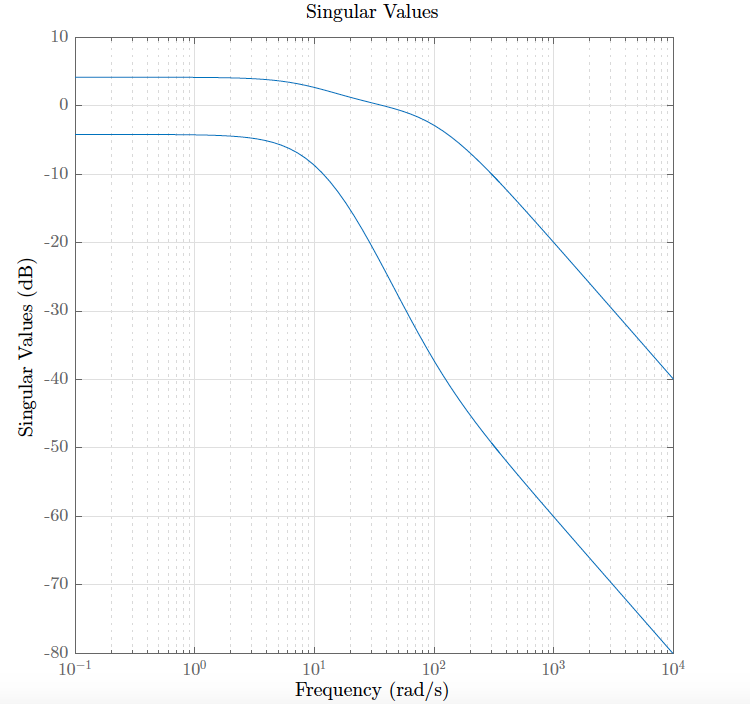
\includegraphics[width=0.6\columnwidth]{phone.png}
\caption{Singular values behaviour.}
\label{fig:phone}
\end{center}
\end{figure}
 \begin{todolist}
  \item $y_\infty(t)=\begin{pmatrix} 
0.5\cdot \sin(30\cdot t+0.314)\\
0.5\cdot \cos(30\cdot t)\\
0.5\cdot \cos(30\cdot t +1)
\end{pmatrix}$.
  \item $y_\infty(t)=\begin{pmatrix} 
4\cdot \sin(30\cdot t+0.314)\\
3\cdot \cos(30\cdot t)\\
2\cdot \cos(30\cdot t +1)
\end{pmatrix}$.
  \item $y_\infty(t)=\begin{pmatrix} 
0.1\cdot \sin(30\cdot t+0.314)\\
0.1\cdot \cos(30\cdot t)\\
0.1\cdot \cos(30\cdot t +1)
\end{pmatrix}$.
  \item $y_\infty(t)=\begin{pmatrix} 
0\\
4\cdot \cos(30\cdot t)\\
2\cdot \cos(30\cdot t +1)
\end{pmatrix}$.
  \item $y_\infty(t)=\begin{pmatrix} 
2\cdot \cos(30\cdot t+0.243)\\
2\cdot \cos(30\cdot t+0.142)\\
2\cdot \cos(30\cdot t +0.252)
\end{pmatrix}$.
  \end{todolist}
  \newpage

\begin{lsg}
\
 \begin{todolist}
  \item  [\done]$y_\infty(t)=\begin{pmatrix} 
0.5\cdot \sin(30\cdot t+0.314)\\
0.5\cdot \cos(30\cdot t)\\
0.5\cdot \cos(30\cdot t +1)
\end{pmatrix}$.
  \item $y_\infty(t)=\begin{pmatrix} 
4\cdot \sin(30\cdot t+0.314)\\
3\cdot \cos(30\cdot t)\\
2\cdot \cos(30\cdot t +1)
\end{pmatrix}$.
  \item $y_\infty(t)=\begin{pmatrix} 
0.1\cdot \sin(30\cdot t+0.314)\\
0.1\cdot \cos(30\cdot t)\\
0.1\cdot \cos(30\cdot t +1)
\end{pmatrix}$.
  \item  [\done]$y_\infty(t)=\begin{pmatrix} 
0\\
4\cdot \cos(30\cdot t)\\
2\cdot \cos(30\cdot t +1)
\end{pmatrix}$.
  \item  [\done]$y_\infty(t)=\begin{pmatrix} 
2\cdot \cos(30\cdot t+0.243)\\
2\cdot \cos(30\cdot t+0.142)\\
2\cdot \cos(30\cdot t +0.252)
\end{pmatrix}$.
  \end{todolist}
  \subsubsection*{Explanation}
  From the given input one can read
  \begin{equation*}
  ||\mu||=\sqrt{3^2+4^2}=5.
  \end{equation*}
  From the plot one can read at $\omega=30\frac{\text{rad}}{\text{s}}$ $\sigma_{min}=0.1$ and $\sigma_{max}=1$. It follows
  \begin{equation*}
  5\cdot \sigma_{min}=0.5\leq ||\nu||\leq 5=5\cdot \sigma_{max}.
  \end{equation*}
  The first response has $||\nu||=\sqrt{0.75}$ that is in the range. The second response has $||\nu||=\sqrt{29}$ that is too big to be in the range. The third response has $||\nu||=\sqrt{0.03}$ that is to small to be in the range. The fourth response has $||\nu||=\sqrt{20}$ that is in the range. The fifth response has $||\nu||=\sqrt{12}$ that is in the range. 

\end{lsg}

\end{bsp}

\newpage 
\section{Synthesis of MIMO Control Systems}
We have learned that MIMO systems are more complicated than SISO systems and therefore their control as well. In fact, it is very difficult to apply intuitive concepts like loop shaping, that apply to SISO systems, because of the cross couplings/interactions between the inputs and the outputs. This means that systematic methods should be used, in order to achieve good control properties. We define two big groups of methods, that are used nowadays:
\begin{itemize}
\item $\mathscr{H}_2$ methods: Optimization problems in time domain which try to minimize the error signal over all frequencies.
\item $\mathscr{H}_\infty$ methods: Optimization problems in frequency domain which try to minimize the error signal over all frequencies.
\end{itemize}
\subsection{The Linear Quadratic Regulator (LQR)}
We first look at one $\mathscr{H}_2$ method: the linear quadratic regulator.
\subsubsection{Definition}
With the given state-space description
\begin{equation}
\frac{\text{d}}{\text{d}t}x(t)=A\cdot x(t)+B\cdot u(t), \qquad A\in\mathbb{R}^{n\times n}, B\in\mathbb{R}^{n\times m},
x(t) \in\mathbb{R}^{n},
u(t) \in\mathbb{R}^{m}
\end{equation}
we are looking for a state-feedback controller
\begin{equation}
u(t)=f(x(t),t),
\end{equation}
that brings $x(t)$ asymptotically   to zero (with $x(0)\neq 0$). In other words it should hold.
\begin{equation}
\lim_{t\to\infty}x(t)=0.
\end{equation}
\begin{bmk}
The input $u(t)$ we want to control depends only on $x(t)$ and not on other dynamic state variables.
\end{bmk}
In order to achieve the best control, we want to minimize the criterium
\begin{equation}\label{krit}
J(x,u)=\int_0^\infty(
\underset{\text{error}}{\underbrace{x^\intercal\cdot Q\cdot x}} +
\underset{\text{{given energy}}}{\underbrace{u^\intercal\cdot R\cdot u}})\,\text{d}t,
\end{equation}
where
\begin{equation}
Q\in\mathbb{R}^{n\times n}
\end{equation}
is a \textit{symmetric positive semidefinite} matrix and
\begin{equation}
\qquad R\in\mathbb{R}^{m\times m}
\end{equation} is a \textit{symmetric positive definite matrix}. These two matrices represent the weights, i.e. the importance, of two things: how fast does the controller bring $x(t)$ to zero and how much energy should it use.\\
\begin{bmk}
In the SISO case, we deal with scalars and things are \textit{nicer}:
\begin{equation}
J(x,u)=\int_0^\infty(
q\cdot x^2+r\cdot u^2)\text{d}t,
\end{equation}

\end{bmk}
\begin{bsp}
Let's try to visualize this: a criterion could look like
\begin{equation*}
J(x,u)=\int_0^\infty \left( x_1^2+6\cdot x_1\cdot x_2+100\cdot x_2^2+6\cdot u_1^2+10\cdot u_2^2 \right)\text{d}t.
\end{equation*}
The matrices $Q$ and $R$ are
\begin{equation*}
Q=\begin{pmatrix}
1&3\\
3&100
\end{pmatrix}
\end{equation*}
and
\begin{equation*}
R=\begin{pmatrix}
6&0\\
0&10
\end{pmatrix}.
\end{equation*}


\end{bsp}
The solution\footnote{Here, it is assumed that $x(t)$ is already available. This is normally not the case and we will therefore introduce an element (observer) that gives us an estimation of it (see next chapters).} $u(t)=f(x(t),t)$ (that minimizes \eqref{krit} ) is given as
\begin{equation}
u(t)=-K\cdot x(t),
\end{equation} with
\begin{equation}
 K=R^{-1}\cdot B^\intercal\cdot \Phi.
\end{equation}
where $\Phi$  is the solution of the Riccati equation
\begin{equation}
\Phi\cdot B\cdot R^{-1}\cdot B^\intercal\cdot \Phi-\Phi\cdot A-A^\intercal\cdot \Phi-Q=0.
\end{equation}
\begin{bmk}
The actual procedure to determine this equation is not trivial. The main point you should be concerned with in this course is the following: we are trying to minimize the given criterium and we are dealing with matrices. This means that in the end, we calculate matrix derivations and minimize, obtaining matrix equations. If you are interested in the minimization procedure have a look \href{https://www.cds.caltech.edu/~murray/courses/cds110/wi06/lqr.pdf}{here}.
\end{bmk}
\begin{bmk}
Don't forget what we are trying to do! This equations give us the optimal controller $K$: this means but not that it will be always the best one.
\end{bmk}
The feedback loop of such a system can be seen in Figure \ref{fig:lqr}. 


\begin{figure}[h]
\begin{center}
\begin{tikzpicture}[auto,node distance=2.5cm]%[auto, node distance=2cm,>=latex']
    \node [input, name=input] {};
    \node [sum, right of=input] (sum) {};
    \node [block, right of=sum] (B) {$B$};
    \node [sum, right of=B] (sum1) {};
    \node [block, right of=sum1] (int) {$\int$};
    \node [block, right of=int,node distance=3cm] (C) {$C$};
    \node [output, right of=C] (output) {};
    \node [block, below of=int,node distance=2 cm] (A) {$A$};
    \node [block, below of=B,node distance=3 cm] (K) {$K$};
  
    \draw [->] (input) -- node {$r(t)=0$} (sum);
    \draw [->] (sum) -- node {} (B);
    \draw [->] (B) |- node {} (sum1);;
    \draw [->] (sum1) -- node {$\dot{x}(t)$} (int);
    \draw [->] (int) -- node [name=x] {$x(t)$} (C);
    \draw [->] (C) -- node {$y$} (output);
    \draw [->] (x) |- node {} (A);
    \draw [->] (A) -| node {} (sum1);
    \draw [->] (x) |- node {} (K);
    \draw [->] (K) -| node {} node[right,pos=0.98] {$-$} (sum);
\end{tikzpicture}
\end{center}
\caption{LQR Problem: Closed loop system.}
\label{fig:lqr}
\end{figure}
\newpage
\subsubsection{Kochrezept}

\begin{enumerate}[(I)]
\item Choose the matrices $Q$ and $R$:
\begin{itemize}
\item The matrix $Q$ is usually chosen as follows: 
\begin{equation}
Q=\bar{C}^T\cdot \bar{C}, \ \bar{C}\in \mathbb{R}^{p\times n}
\label{fullr}
\end{equation}
where
\begin{equation}
p=\text{rank}(Q)\leq n.
\end{equation}
Equation \ref{fullr} represents the \textbf{full-rank} decomposition of $Q$. This makes sure that the therm with $Q$ in the criterion contains enough informations about the state's behaviour. $\bar{C}$ has strictly speaking nothing to do with the state space description's matrix $C$. We will however discover, that the choice $\bar{C}=C$ is really interesting.
\item The matrix $R$ is usually chosen as follows:
\begin{equation}
R=r\cdot \mathbb{1}_{m\times m}.
\end{equation}
\end{itemize}
\item Find the \textbf{symmetric, positive definite} solution $\Phi$ of the Riccati equation
\begin{equation}
\Phi\cdot B\cdot R^{-1}\cdot B^\intercal\cdot \Phi-\Phi\cdot A-A^\intercal\cdot \Phi-Q=0.
\end{equation}
\begin{bmk}
Such a solution exists if
\begin{itemize}
\item The pair $\{ A,B\}$ is completely controllable and
\item The pair $\{ A,\bar{C}\}$ is completely observable.
\end{itemize}
This doesn't mean that these conditions should be always fulfilled: \textbf{sufficient, not necessary.}
\end{bmk}
\item Compute the matrix of the controller $K$ with
\begin{equation}
 K=R^{-1}\cdot B^\intercal\cdot \Phi.
\end{equation}
\end{enumerate}
\subsubsection{Frequency Domain}
By looking at Figure \ref{fig:lqr} one can write
\begin{equation}
L_{\text{LQR}}(s)=K\cdot (s\cdot \mathbb{1}-A)^{-1}\cdot B
\end{equation}
and
\begin{equation}
T_{\text{LQR}}(s)=C\cdot (s\cdot \mathbb{1}-(A-B\cdot K))^{-1}\cdot B.
\end{equation}
\subsubsection{Properties}
A bunch of nice properties can be listed:
\begin{itemize}
\item The matrix of the closed-loop system 
\begin{equation}
A-B\cdot K
\end{equation}
is guaranteed to be a \textbf{Hurwitz} matrix.
\begin{bmk}
A Hurwitz matrix is a matrix that has all eigenvalues with \textit{negative} real parts.
\end{bmk}
But wait, what does it mean? We have learned that eigenvalues with negative real parts contribute to the stability of the closed-loop system. In this case is the closed-loop system \textbf{asymptotically stable}.
\item If one chooses $R=r\cdot \mathbb{1}$ one gets for the minimal return difference
\item If $Q>> R$ we say that we have \textbf{cheap control energy}.
\item If $R>> Q$ we say that we have \textbf{expensive control energy}.

\begin{equation}
\mu_{\text{LQR}}=\min_\omega\{\sigma_{\text{min}}(\mathbb{1}+L_{LQR})\}\geq 1.
\end{equation}
\item Closed-loop behaviour:
\begin{align}
\max_\omega\{\sigma_{\text{max}}(S(j\cdot\omega))\}&\leq 1, \\
\max_\omega\{\sigma_{\text{max}}(T(j\cdot\omega))\}&\leq 2.
\end{align}

\item Of course you are not expected in real life to solve the Riccati equation by hand. Since these calculations contain many matrix multiplications, numerical algorithms are developed. \textsc{Matlab} offers the command
\begin{verbatim}
K=lqr(A,B,Q,R);
\end{verbatim}
\item Remind that 
\begin{equation}
\Phi=\Phi^T.
\end{equation}
\end{itemize}

\subsubsection{Pole Placement}
Another intuitive way of approaching this problem is the so called \textit{pole placement}. Given that one knows that the state feedback matrix is $A-B\cdot K$, one can choose such a $K$ matrix, that the desired poles are achieved. With this method one can have direct influence on the speed of the control system. The disadvantage, however, is that one has no guarantee of robustness. If one looks at Figure \ref{fig:statecontr}, one can derive the following complete state space description of the plant and of the controller:

\begin{equation}
\begin{split}
\dot{x}(t)&=A\cdot x(t)+B\cdot u(t),\\
y(t)&=C\cdot x(t)+D\cdot u(t),\\
\dot{z}(t)&=F\cdot z(t)+G\cdot e(t),\\
u(t)&=H\cdot z(t),
\end{split}
\end{equation}
where $e(t)$ is the error of the controller.
\subsubsection*{Open Loop Conditions}
By assuming for this case $D=0$ and plugging the information of the controller in the plant, one gets
\begin{equation}
\begin{split}
\dot{x}(t)&=A\cdot x(t)+B\cdot H\cdoz z(t),\\
y(t)&=C\cdot x(t),\\
\dot{z}(t)&=F\cdot z(t)+G\cdot e(t).
\end{split}
\end{equation}
By defining two new variables $\tilde{x}(t)=\begin{pmatrix} x(t)\\z(t) \end{pmatrix}$, $\tilde{u}(t)=\begin{pmatrix} u(t)\\e(t) \end{pmatrix}$ and referring to Figure \ref{fig:controp} one can write
\begin{equation}
\begin{split}
A_{\text{open loop}}&=\begin{pmatrix} A & B\cdot H \\
0&F
\end{pmatrix},\\
B_{\text{open loop}}&=\begin{pmatrix} 0 \\
G
\end{pmatrix},\\
C_{\text{open loop}}&=\begin{pmatrix} C &0
\end{pmatrix}.
\end{split}
\end{equation}
\begin{bmk}
Because of the rule for determinant of matrices build up from other submatrices, we automatically know that the eigenvalues of $A_{\text{open loop}}$ are the eigenvalues of $A$ and the eigenvalues of $F$. Mathematically
\begin{equation}
\lambda (A_{\text{open loop}})=\lambda(A)+\lambda(F).
\end{equation}
\end{bmk}
\subsubsection*{Closed Loop Conditions}
It is still assumed $D=0$. If one closes the loop it holds
\begin{equation}
e(t)=-y(t) \Rightarrow \ e(t)=-C\cdot x(t).
\end{equation}
This gives the state space description
\begin{equation}
\begin{split}
\dot{x}(t)&=A\cdot x(t)+B\cdot H\cdoz z(t),\\
y(t)&=C\cdot x(t),\\
\dot{z}(t)&=F\cdot z(t)+G\cdot (-C\cdot x(t)).
\end{split}
\end{equation}
By defining a new variable $\tilde{x}(t)=\begin{pmatrix} x(t)\\z(t) \end{pmatrix}$ and referring to Figure \ref{fig:contrcl} one can write
\begin{equation}
A_{\text{closed loop}}=\begin{pmatrix} A & B\cdot H \\
-G\cdot C&F
\end{pmatrix}.
\end{equation}
\begin{bmk}
The eigenvalues of $A_{\text{closed loop}}$ are not well defined. Moreover it holds
\begin{equation}
\lambda(A_{\text{closed loop}})=f(F,G,H).
\end{equation}
This makes this method extremely superficial and not generally useful.
\end{bmk}

\begin{figure}[h!]
\begin{center}
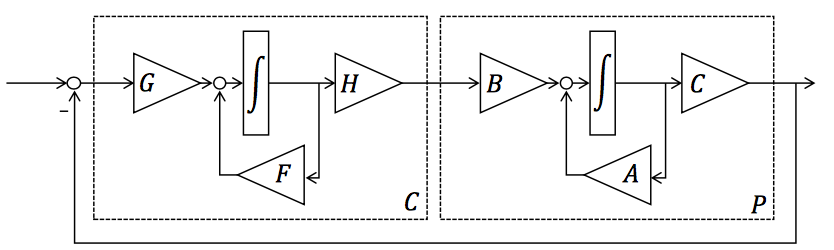
\includegraphics[width=0.7\columnwidth]{statecontr.png}
\caption{Signal Flow Diagram with Controller.}
\label{fig:statecontr}
\end{center}
\end{figure}

\begin{figure}[h!]
\begin{center}
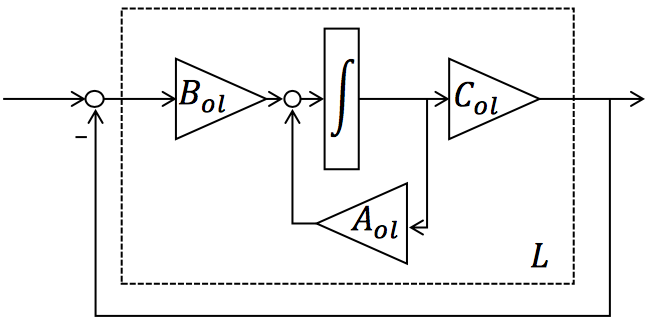
\includegraphics[width=0.4\columnwidth]{controp.png}
\caption{Open loop case.}
\label{fig:controp}
\end{center}
\end{figure}

\begin{figure}[h]
\begin{center}
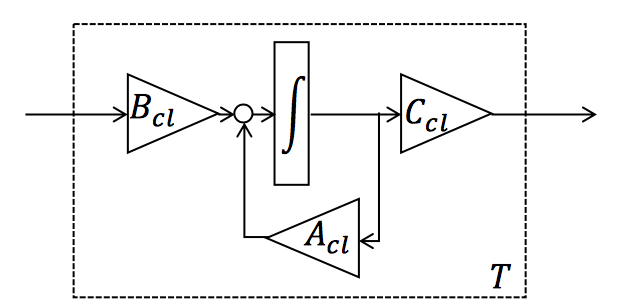
\includegraphics[width=0.4\columnwidth]{contrcl.png}
\caption{Closed loop case.}
\label{fig:contrcl}
\end{center}
\end{figure} 
\pagebreak



\subsubsection{Examples}
\begin{bsp}
Your task is to keep a space shuttle in its trajectory . The deviations from the desired trajectory are well described by
\begin{equation*}
\begin{split}
 \dd{}{t} x(t) &= A \cdot x(t) + b \cdot u(t) \\
&= \begin{pmatrix} 0&1\\ 0&0 \end{pmatrix} \cdot x(t) + \begin{pmatrix} 0\\ 1\end{pmatrix} \cdot u(t). \\
 \end{split}
\end{equation*}
$x_1(t)$ is the position of the space shuttle and $x_2(t)$ is its velocity. Moreover, $u(t)$ represents the propulsion. The position and the velocity are known for every moment and for this reason we can use a state-feedback regulator. In your first try, you want to implement a LQR with
\begin{equation*}
\begin{split}
Q&=\begin{pmatrix}
1&0\\
0&2.25
\end{pmatrix}\\
R&=4.
\end{split}
\end{equation*}
\begin{enumerate}[(a)]
\item Show that the system is completely controllable.
\item Find the state feedback matrix $K$.
\end{enumerate}
After some simulations, you decide that the controller you've found is not enough for your task. Your boss doesn't want you to change the matrices $Q$ and $R$ and for this reason you decide to try with direct pole placement. The specifications are
\begin{itemize}
\item The system should not overshoot.
\item The error of the regulator should decrease with $e^{-3\cdot t}$.
\end{itemize}
\begin{enumerate}[(c)]
\item Find the poles such that the specifications are met.
\end{enumerate}
\begin{enumerate}[(d)]
\item Find the new state feedback matrix $K_2$.
\end{enumerate}


\newpage
\begin{lsg}
\
\begin{enumerate}[(a)]
\item The controllybility of the system is easy to show: the controllability matrix is
\begin{equation*}
\begin{split}
R_2&=\begin{pmatrix}
b & A\cdot b
\end{pmatrix}\\
&=\begin{pmatrix}
0&1\\
1&0
\end{pmatrix}.
\end{split}
\end{equation*}
The rank of $R$ is clearly 2: completely controllable.
\item In order to find the matrix $K$, one has to compute the solution of the Riccati equation related to this problem. First, one has to look at the form that this solution should have. Here $b$ is a $2\times 1$ vector. This means that since $\Phi=\Phi^T$ we are dealing with a $2\times 2$ $\Phi$ of the form
\begin{equation*}
\Phi=\begin{pmatrix}
\varphi_1 & \varphi_2\\
\varphi_2 & \varphi_3
\end{pmatrix}
\end{equation*}
With the Riccati equation, it holds
\begin{equation*}
\Phi\cdot B\cdot R^{-1}\cdot B^\intercal\cdot \Phi-\Phi\cdot A-A^\intercal\cdot \Phi-Q=0
\end{equation*}
Plugging in the matrices one gets
\begin{equation*}
\begin{split}
\Phi \cdot \begin{pmatrix} 0\\ 1\end{pmatrix}\cdot 4^{-1}\cdot \begin{pmatrix} 0\\ 1\end{pmatrix}^T\cdot \Phi -\Phi \cdot \begin{pmatrix} 0&1\\ 0&0 \end{pmatrix}
-\begin{pmatrix} 0&1\\ 0&0 \end{pmatrix}^T\cdot \Phi -\begin{pmatrix}
1&0\\
0&2.25
\end{pmatrix}&=\begin{pmatrix} 0&0\\ 0&0 \end{pmatrix}\\
\frac{1}{4}\cdot \begin{pmatrix}
\varphi_2\\
\varphi_3
\end{pmatrix}\cdot \begin{pmatrix} 0&1\end{pmatrix}\cdot \begin{pmatrix}
\varphi_1 & \varphi_2\\
\varphi_2 & \varphi_3
\end{pmatrix}
- \begin{pmatrix}0&\varphi_1\\0&\varphi_2 \end{pmatrix} - 
\begin{pmatrix}
0&0\\
\varphi_1 & \varphi_2 
\end{pmatrix}-\begin{pmatrix}
1&0\\
0&2.25
\end{pmatrix}&=\begin{pmatrix} 0&0\\ 0&0 \end{pmatrix}\\
\frac{1}{4}\cdot \begin{pmatrix}
 0&\varphi_2\\
 0&\varphi_3
 \end{pmatrix}\cdot \begin{pmatrix}
\varphi_1 & \varphi_2\\
\varphi_2 & \varphi_3
\end{pmatrix}
 -\begin{pmatrix}
1&\varphi_1 \\
\varphi_1 & 2\cdot \varphi_2+2.25
\end{pmatrix}&=\begin{pmatrix} 0&0\\ 0&0 \end{pmatrix}\\
\frac{1}{4}\cdot
\begin{pmatrix}
\varphi_2^2&\varphi_2 \cdot \varphi_3\\
\varphi_2 \cdot \varphi_3 &\varphi_3^2
\end{pmatrix}-\begin{pmatrix}
1&\varphi_1 \\
\varphi_1 & 2\cdot \varphi_2+2.25
\end{pmatrix}&=\begin{pmatrix} 0&0\\ 0&0 \end{pmatrix}\\
 \begin{pmatrix}
\frac{\varphi_2^2}{4}-1&\frac{\varphi_2\cdot \varphi_3}{4}-\varphi_1\\[6pt]
\frac{\varphi_2\cdot \varphi_3}{4}-\varphi_1 &\frac{\varphi_3^2}{4}-2\cdot \varphi_2-2.25
\end{pmatrix}&=\begin{pmatrix}0&0\\ 0&0\end{pmatrix}.
\end{split}
\end{equation*}
From this it follows:
\begin{itemize}
\item $\frac{\varphi_2^2}{4}-1$ $ \Rightarrow$ $\varphi_2=\pm 2$. 
\item From the fourth term, we get two cases:
\begin{itemize}
\item $\varphi_2=2$: $\varphi_3=\sqrt{25}=\pm 5$.
\item $\varphi_2=-2$: $\varphi_3=j\cdot \sqrt{7}$. 
\end{itemize}
 \item Because of the \textit{Sylvester's Criterion}, $\varphi_1$ should be positive, in order to get a positive definite matrix. Plugging into the second term: $\varphi_1=\frac{\varphi_2\cdot \varphi_3}{4}=2.5$ is the only positive solution. This means that the only reasonable choice is $\varphi_2=2$ and $\varphi_3=5$.
\end{itemize}
We therefore get
\begin{equation*}
\Phi=\begin{pmatrix} 2.5&2\\ 2&5\end{pmatrix}.
\end{equation*}
Because of the \textit{Sylvester's Criterion} and the fact that $\Phi$ should be positive definite, this is a good matrix! \\
For the matrix $K$ it holds
\begin{equation*}
\begin{split}
 K&=R^{-1}\cdot B^\intercal\cdot \Phi\\
 &=\frac{1}{4}\cdot \begin{pmatrix} 0& 1 \end{pmatrix} \cdot \begin{pmatrix} 2.5&2\\ 2&5\end{pmatrix}\\
 &= \frac{1}{4}\cdot \begin{pmatrix} 2&5\end{pmatrix}.
 \end{split}
\end{equation*}
\item Overshoot or in general oscillations, are due to the complex part of some poles. The real part of these poles is given by the decrease function of the error: $$\pi_1=\pi_2=-3$$
\item The closed loop has feedback matrix 
$$A-B\cdot K_2.$$
We have to choose $K_2$ such that the eigenvalues of the state feedback matrix are both $-3$. The dimensions of $K_2$ are the same as the dimensions of $K$, namely $1\times 2$. It holds
\begin{equation*}
\begin{split}
A-B\cdot K_2&=\begin{pmatrix} 0&1\\ 0&0 \end{pmatrix} -\begin{pmatrix} 0\\ 1 \end{pmatrix} \cdot \begin{pmatrix}k_1& k_2 \end{pmatrix}\\
&= \begin{pmatrix} 0&1\\ 0&0 \end{pmatrix}-\begin{pmatrix} 0&0\\ k_1 & k_2 \end{pmatrix}\\
&=\begin{pmatrix}
0&1\\ -k_1&-k_2
\end{pmatrix}.
\end{split}
\end{equation*}
The eigenvalues of this matrix are
\begin{equation*}
\pi_{1,2}=\frac{-k_2\pm \sqrt{k_2^2-4k_1}}{2}.\\
\end{equation*}
Since the two eigenvalues should have the same value, we know the the part under the square rooth should vanish. This means that $-\frac{k_2}{2}=-3 \Rightarrow k_2=6$. Moreover:
\begin{equation*}
\begin{split}
k_1&=\frac{k_2^2}{4}\\
&=9.
\end{split}
\end{equation*}
The matrix finally reads
\begin{equation*}
K_2=\begin{pmatrix} 9&6\end{pmatrix}.
\end{equation*}
\end{enumerate}
\end{lsg}
\end{bsp}
\newpage


\begin{bsp}
A system is given as
\begin{equation*}
\begin{split}
\dot{x}_1&=3\cdot x_2\\
\dot{x}_2&=3\cdot x_1-2\cdot x_2 + \frac{1}{2} \cdot u\\
y&=4\cdot x_1+\frac{7}{3} \cdot x_2.
\end{split}
\end{equation*}
\begin{enumerate}[(a)]
\item Solve the LQR problem for the criterion
\begin{equation*}
J=\int_0^\infty 7\cdot x_1^2+3\cdot x_2^2+\frac{1}{4}\cdot u^2 \text{d}t
\end{equation*}
and find $K$.
\item Find the eigenvalues of the closed-loop and the LQ regulator $K$.
\item Does it change something if we use the new criterion?
\begin{equation*}
J_{\text{new}}=\int_0^\infty 70\cdot x_1^2+30\cdot x_2^2+\frac{10}{4}\cdot u^2 \text{d}t.
\end{equation*}

\end{enumerate}


\newpage
\begin{lsg}
\
\begin{enumerate}[(a)]
\item 
From the theory of the course $\textit{Lineare Algebra I/II}$ about the quadratic forms, one can read
\begin{equation*}
Q=\begin{pmatrix}
7&0\\ 0&3
\end{pmatrix}
\end{equation*}
and
\begin{equation*}
R=\frac{1}{4}.
\end{equation*}
The state-space description of the system can be rewritten as
\begin{equation*}
\begin{split}
\begin{pmatrix} 
\dot{x}_1\\ \dot{x}_2
\end{pmatrix}&=\underbrace{\begin{pmatrix} 0&3 \\ 3&-2 
\end{pmatrix}}_{A}\cdot \begin{pmatrix} x_1\\ x_2 
 \end{pmatrix}+ \underbrace{\begin{pmatrix} 0\\  \frac{1}{2} 
 \end{pmatrix}}_{B}\cdot u\\
 y&=\underbrace{\begin{pmatrix} 4&\frac{7}{3}
\end{pmatrix}}_{C}\cdot \begin{pmatrix} x_1\\ x_2 
 \end{pmatrix}+\underbrace{0}_{D}\cdot u.
\end{split}
\end{equation*}
Plugging this into the Riccati equation one gets:
\begin{equation*}
\begin{split}
\Phi \cdot \begin{pmatrix} 0\\  \frac{1}{2} 
 \end{pmatrix}\cdot 4 \cdot \begin{pmatrix} 0&  \frac{1}{2} 
 \end{pmatrix}\cdot \Phi-\Phi \cdot \begin{pmatrix} 0&3 \\ 3&-2 
\end{pmatrix}-\begin{pmatrix} 0&3 \\ 3&-2 
\end{pmatrix}\cdot \Phi-\begin{pmatrix}
7&0\\ 0&3
\end{pmatrix}&=\begin{pmatrix} 0&0 \\ 0&0 \end{pmatrix}\\
\begin{pmatrix}
2 \varphi_2 \\
2 \varphi_3
\end{pmatrix}\cdot 
\begin{pmatrix}
\frac{\varphi_2}{2}&\frac{\varphi_3}{2}
\end{pmatrix}-\begin{pmatrix}
3 \varphi_2 & 3  \varphi_1-2 \varphi_2\\
3 \varphi_3 &3 \varphi_2-2 \varphi_3
\end{pmatrix}-\begin{pmatrix}
3 \varphi_2 & 3 \varphi_3\\
3 \varphi_1 -2 \varphi_2 &3 \varphi_2-2 \varphi_3
\end{pmatrix}-\begin{pmatrix}
7&0\\ 0&3
\end{pmatrix}&=\begin{pmatrix} 0&0 \\ 0&0 \end{pmatrix}\\
 \begin{pmatrix}
\varphi_2^2 & \varphi_2 \varphi_3\\
\varphi_2 \varphi_3 & \varphi_3^2
 \end{pmatrix}-\begin{pmatrix}
6 \varphi_2 +7 &3 \varphi_1 -2 \varphi_2 +3 \varphi_3 \\
3 \varphi_1 -2 \varphi_2 +3 \varphi_3 &6 \varphi_2-4 \varphi_3+3
\end{pmatrix}&=\begin{pmatrix} 0&0 \\ 0&0 \end{pmatrix}.
\end{split}
\end{equation*}
Hence, one gets 3 equations (two elements are equal because of symmetry):
\begin{equation*}
\begin{split}
\varphi_2^2-6\cdot \varphi_2 -7 &=0\\
\varphi_2\cdot \varphi_3-3\cdot \varphi_1 +2\cdot \varphi_2 -3\cdot \varphi_3 &=0\\
\varphi_3^2-6\cdot \varphi_2+4\cdot \varphi_3-3&=0.
\end{split}
\end{equation*}
From here, with the same procedure we have used before, one gets
\begin{equation*}
\Phi=\begin{pmatrix}
\frac{34}{3}&7\\
7&5
\end{pmatrix}.
\end{equation*}
This gives $K$ as
\begin{equation*}
\begin{split}
K&=4\cdot \begin{pmatrix} 0&\frac{1}{2} \end{pmatrix} \cdot \begin{pmatrix}
\frac{34}{3}&7\\
7&5
\end{pmatrix}\\
&=\begin{pmatrix}
14&10 
\end{pmatrix}.
\end{split}
\end{equation*}
\item The matrix to analyze is
\begin{equation*}
\begin{split}
A-B\cdot K&=\begin{pmatrix} 0&3 \\ 3&-2 
\end{pmatrix}-\begin{pmatrix}
0\\ \frac{1}{2}
\end{pmatrix}\cdot \begin{pmatrix}
14&10 
\end{pmatrix}\\
&=\begin{pmatrix} 0&3 \\ 3&-2 
\end{pmatrix}- \begin{pmatrix}
 0&0\\
 7&5\\
 \end{pmatrix}\\
&=\begin{pmatrix} 0&0\\
-4&-7
\end{pmatrix}.
\end{split}
\end{equation*}
The eigenvalues of the closed loop system are given with
\begin{equation*}
\begin{split}
\det((A-B\cdot K)-\lambda \cdot \mathbb{1})&=0\\
\lambda^2+7\lambda +12&=0
\end{split}
\end{equation*}
from which it follows: $\lambda_1=-3$ and $\lambda_2=-4$.
\item No. $K$ remains the same, because it holds $J_{\text{new}}=10\cdot J$. 

\end{enumerate}
\end{lsg}

\end{bsp}
\newpage
\begin{bsp}
\
You have to design a LQ regulator for a plant with 2 inputs, 3 outputs and 6 state variables.
\begin{enumerate}[(a)]
\item What are the dimensions of $A$, $B$, $C$ and $D$?
\item What is the dimension of the transfer function $u\rightarrow y$?
\item What is the dimension of the matrix $Q$ of $J_{LQR}$?
\item What is the dimension of the matrix $R$ of $J_{LQR}$?
\item What is the dimension of the matrix $K$?
\end{enumerate}
\newpage
\begin{lsg}
\
\begin{enumerate}[(a)]
\item One can find the solution by analyzing the meaning of the matrices:
\begin{itemize}
\item Since we are given 6 states variables, the matrix $A$ should have 6 rows and 6 columns, i.e. $A\in \mathbb{R}^{6\times6}$.
\item Since we are given 2 inputs, the matrix $B$ should have 2 columns and 6 rows, i.e. $B\in \mathbb{R}^{6\times2}$.
\item Since we are given 3 outputs, the matrix $C$ should have 6 columns and 3 rows, i.e. $C\in \mathbb{R}^{3\times6}$.
\item Since we are given 2 inputs and 3 outputs, the matrix $D$ should have 2 columns and 3 rows, i.e. $D\in \mathbb{R}^{3\times2}$.
\end{itemize}
\item Since we are dealing with a system with 2 inputs and 3 outputs, $P(s)\in \mathbb{R}^{3\times2}$. Moreover, $P(s)$ should have the same dimensions of $D$ because of its formula.
\item From the formulation of $Q$ one can easily see that its dimensions are the same of the dimensions of $A$, i.e. $Q \in \mathbb{R}^{6\times6}$.
\item From 
$$u(t)=-K\cdot x(t).$$
we can see that $K$ should have 6 columns and 2 rows, i.e. $K\in \mathbb{R}^{2\times6}$.
\end{enumerate}

\end{lsg}

\end{bsp}


\newpage

\begin{bsp}
You design with \textsc{Matlab} a LQ Regulator:
\begin{verbatim}
1  A = [1 0 0 0; 1 1 0 0; 1 1 1 0;  0 0 1 1];
2  B = [1 1 1 1; 0 1 0 2];
3  C = [0 0 0 1; 0 0 1 1; 0 1 1 1];
4
5  nx = size(A,1); Number of state variables of the plant, in Script: n
6  nu = size(B,2); Number of input variables of the plant, in Script: m
7  ny = size(C,1); Number of output variables of the plant, in Script: p
8 
9  q = 1;
10 r = 1;
11 Q = q*eye(###);
12 R = r*eye(###);
13
14 K = lqr(A,B,Q,R);

\end{verbatim}
Fill the following rows:\\
\begin{verbatim}
11  : ### = 
12  : ### = 
\end{verbatim}
\newpage
\begin{lsg}
The matrix $Q$ is a weight for the states and the matrix $R$ is a weight for the inputs. The correct filling is
\begin{verbatim}
11  : ### = nx 
12  : ### = nu
\end{verbatim}
\end{lsg}

\end{bsp}
\newpage

\subsection{Extensions of the LQR problem}
\subsubsection{The LQRI}
This is an extension of what was presented in the previous section. In the previous formulation, \textbf{no integral action} was present: in this section we introduce it. The main idea is to introduce a (P)I element to each output channel, in order to control the static error.
\subsubsection*{Definition} Two possible structure's representations can be seen in Figure \ref{fig:lqri1} and Figure \ref{fig:lqri2}. Let's analyze this system by referring to Figure \ref{fig:lqri2}. Let's define a new state vector 
\begin{equation}
\tilde{x}(t)=\begin{pmatrix} x(t) \\ v(t) \end{pmatrix} \ \in \mathbb{R}^{n+m}.
\end{equation}
Two assumptions are then used:
\begin{itemize}
\item $D=0$,
\item we have the same number of inputs and outputs (square systems).
\end{itemize}
By subdividing different $B$ matrices for $u(t)$, $w(t)$ and $r(t)$ one gets the dynamics
\begin{equation}
\frac{\text d}{\text{d}t}\tilde x(t)=\tilde A \cdot \tilde x(t)+ \tilde B_u\cdot u(t)+\tilde B_r \cdot r(t)+\tilde B_w \cdot w(t),
\end{equation}
where
\begin{equation}
\tilde A=\begin{bmatrix} A & 0 \\ -C & 0 \end{bmatrix}, \qquad
\tilde B_u=\tilde B_w=\begin{bmatrix} B \\ 0 \end{bmatrix}, \qquad 
\tilde B_r=\begin{bmatrix} 0 \\ \mathbb{1} \end{bmatrix}.
\end{equation}
This can be solved using the LQR approach and the new weight matrices
\begin{equation}
\begin{split}
\tilde{C}&=\begin{pmatrix} \bar{C}&0\\ 0&\gamma \cdot \mathbb{1} \end{pmatrix}\\
\Rightarrow \tilde{Q}&=\tilde{C}^T\cdot \tilde{C}\\
&=\begin{pmatrix}
Q&0\\
0&\gamma^2 \cdot \mathbb{1}
\end{pmatrix}.
\end{split}
\end{equation}
and
\begin{equation}
\tilde{R}=R.
\end{equation}
The solution we want to find is then
\begin{equation}
\tilde{K}=\begin{pmatrix} 
K&-K_I
\end{pmatrix},
\end{equation}
where $K\in \mathbb{R}^{m\times n}$ and $K_I\in \mathbb{R}^{m\times p}$.
\begin{bmk}
\
\begin{itemize}
\item One could ask, why the matrix $R$ is unchanged. Recalling the role of $R$, one sees that it is the weight for the input, that remains unchanged with respect to the initial LQR problem. 
\item $\gamma >0$ is the tuning parameter, that defines how strong will the integral action be.
\end{itemize}
\end{bmk}




\begin{figure}[h]
\begin{center}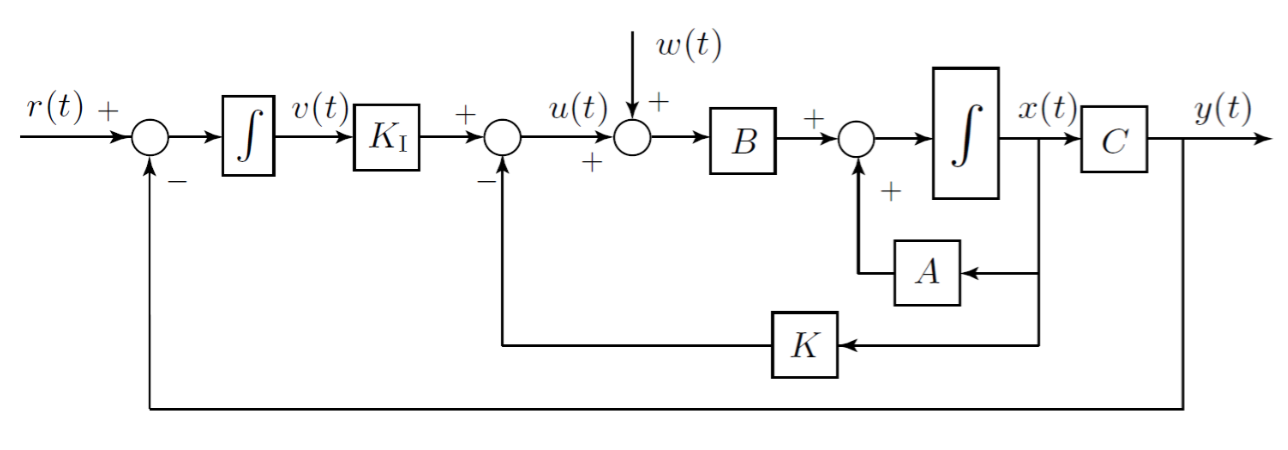
\includegraphics[width=0.8\columnwidth]{LQRI1}\end{center}
\caption{Structure of LQRI.}
\label{fig:lqri1}
\end{figure}

\begin{figure}[h]
\begin{center}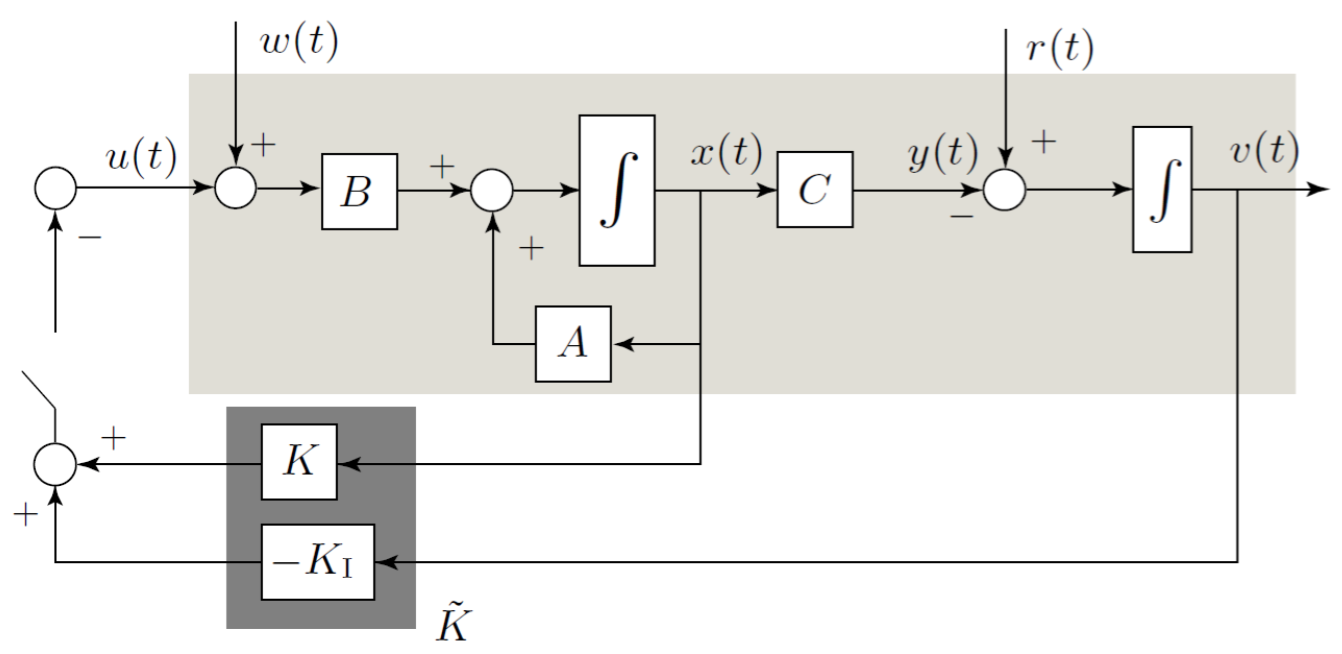
\includegraphics[width=0.7\columnwidth]{LQRI2}\end{center}
\caption{Structure of LQRI.}
\label{fig:lqri2}
\end{figure}

\subsubsection*{Kochrezept}
\begin{enumerate}[(I)]
\item Define the new system 
\begin{equation}
\frac{\text d}{\text{d}t}\tilde x(t)=\tilde A \cdot \tilde x(t)+ \tilde B_u\cdot u(t)+\tilde B_r \cdot r(t)+\tilde B_w \cdot w(t), \ \tilde{x}(t)=\begin{pmatrix} x(t) \\ v(t) \end{pmatrix}.
\end{equation}
with 
\begin{equation}
\tilde A=\begin{bmatrix} A & 0 \\ -C & 0 \end{bmatrix}, \qquad
\tilde B_u=\tilde B_w=\begin{bmatrix} B \\ 0 \end{bmatrix}, \qquad 
\tilde B_r=\begin{bmatrix} 0 \\ \mathbb{1} \end{bmatrix}.
\end{equation}
\item Choose the desired weight matrices 
\begin{equation}
\tilde{Q}=\begin{pmatrix}
Q&0\\
0&\gamma^2 \cdot \mathbb{1}
\end{pmatrix}, \ \tilde R=R.
\end{equation}
The controller is then 
\begin{equation}
\tilde{K}=\begin{pmatrix} 
K&-K_I
\end{pmatrix},
\end{equation}
\item Find $\tilde{K}$ using the standard LQR formulation with $\{ \tilde{A},\tilde{B}_u,\tilde{Q},\tilde{R} \}$ instead of $\{A,B,Q,R\}$.
\item Use the \textsc{Matlab} command
\begin{verbatim}
K_tilde=lqr(A_tilde,B_u_tilde,C_tilde'*C_tilde,r*eye(m,m)).
\end{verbatim}
\end{enumerate}
\newpage
\subsubsection*{Examples}
\begin{bsp}
The dynamics of a system are given as
\begin{equation*}
\begin{split}
\dot{x}(t)&=3\cdot x(t)+2\cdot u(t)\\
y(t)&=2\cdot x(t).
\end{split}
\end{equation*}
First, you try to solve the problem by using the standard LQR problem statement. However,after some measurements, you notice that the controller you've found actually is not so good: there is a stationary controller's error. You decide to use the LQRI formulation, in order to eliminate this error. Find the new controller $K_e$ using $R=1$, $\bar{C}=2$ and integral action $\gamma=1$.
\newpage

\begin{lsg}
The matrices that describe the dynamics of the system are
\begin{equation*}
\begin{split}
A&=(3),\\
B&=(2),\\
C&=(2).
\end{split}
\end{equation*}
The new matrices $\{\tilde{A},\tilde{B},\tilde{C} \}$ are
\begin{equation*}
\begin{split}
\tilde{A}&=\begin{pmatrix} A&0\\-C&0 \end{pmatrix}\\
&=\begin{pmatrix} 3&0\\-2&0\end{pmatrix},\\
\tilde{B}&=\begin{pmatrix} B\\ 0 \end{pmatrix}\\
&=\begin{pmatrix} 2\\ 0\end{pmatrix},\\
\tilde{C}&=\begin{pmatrix} \bar{C}&0 \\ 0&\gamma \cdot \mathbb{1} \end{pmatrix} \\
&=\begin{pmatrix} 2&0\\ 0&1 \end{pmatrix}.
\end{split}
\end{equation*}
The matrix $\tilde{Q}$ reads
\begin{equation*}
\begin{split}
\tilde{Q}&=\bar{C}^T\cdot \bar{C}\\
&=\begin{pmatrix} 2&0\\ 0&1 \end{pmatrix}^2\\
&=\begin{pmatrix} 4&0\\ 0&1 \end{pmatrix}.
\end{split}
\end{equation*}
With $\Phi=\begin{pmatrix} \varphi_1 & \varphi_2 \\ \varphi_2 & \varphi_3 \end{pmatrix}$ one gets for the Riccati equation:
\begin{equation*}
\begin{split}
\Phi\cdot \tilde{B}\cdot \tilde{R}^{-1}\cdot \tilde{B}^\intercal\cdot \Phi-\Phi\cdot \tilde{A}-\tilde{A}^\intercal\cdot \Phi-\tilde{Q}&=0\\
\Phi \cdot \begin{pmatrix} 2\\ 0\end{pmatrix} \cdot 1 \cdot \begin{pmatrix} 2& 0\end{pmatrix}\cdot \Phi - \Phi \cdot \begin{pmatrix} 3&0\\-2&0\end{pmatrix} -\begin{pmatrix} 3&-2\\ 0&0\end{pmatrix}\cdot \Phi - \begin{pmatrix} 4&0\\ 0&1 \end{pmatrix}&=\begin{pmatrix} 0&0 \\ 0&0 \end{pmatrix}\\
\begin{pmatrix} 4\varphi_1^2 & 4\varphi_1 \varphi_2 \\ 4\varphi_1 \varphi_2 & 4\varphi_2^2 \end{pmatrix} - \begin{pmatrix} 3\varphi_1-2\varphi_2 &0 \\ 3\varphi_2-2\varphi_3 &0 \end{pmatrix} -\begin{pmatrix} 3\varphi_1-2\varphi_2 & 3\varphi_2-2\varphi_3\\ 0 &0 \end{pmatrix}-\begin{pmatrix} 4&0\\ 0&1 \end{pmatrix}&=\begin{pmatrix} 0&0 \\ 0&0 \end{pmatrix}\\
\begin{pmatrix} 
4\varphi_1^2-6\varphi_1+4\varphi_2-4 & 4\varphi_1 \varphi_2 - 3\varphi_2+2\varphi_3\\
4\varphi_1 \varphi_2 - 3\varphi_2+2\varphi_3 & 4\varphi_2^2-1 
\end{pmatrix}&=\begin{pmatrix} 0&0 \\ 0&0 \end{pmatrix}.
\end{split}
\end{equation*}
Let's now analyze the equations:
\begin{itemize}
\item From the fourth term of the matrix, one can compute $\varphi_2$. One gets $\varphi_2=\pm \frac{1}{2}$. 
\item By plugging these two into the first term of the equation one can get the following results:
\begin{itemize}
\item $\varphi_2=\frac{1}{2}$, from which it follows $\varphi_1=\frac{3\pm \sqrt{17}}{4}$.
\item $\varphi_2=-\frac{1}{2}$, from which it follows $\varphi_1=\frac{3\pm \sqrt{33}}{4}$.
\end{itemize}

Because of the Sylvester's criterion, one has to eliminate all negative solutions for $\varphi_1$. This means we are left with two solutions:
\begin{itemize}
\item $\varphi_2=\frac{1}{2}$, $\varphi_1=\frac{3+\sqrt{17}}{4}$.
\item $\varphi_2=-\frac{1}{2}$, $\varphi_1=\frac{3+\sqrt{33}}{4}$.
\end{itemize}
\item Let's plug these solutions into the second term of the equation, where $\varphi_3=\frac{-4\varphi_1 \varphi_2 +3 \varphi_2}{2}$:
\begin{itemize}
\item $\varphi_2=\frac{1}{2}$, $\varphi_1=\frac{3+\sqrt{17}}{4}$, from which it follows 
\begin{equation*}
\begin{split}
\varphi_3&=-\frac{3+\sqrt{17}}{4}+\frac{3}{4}\\
&=-\frac{\sqrt{17}}{4}.
\end{split}
\end{equation*}
\item $\varphi_2=-\frac{1}{2}$, $\varphi_1=\frac{3+\sqrt{33}}{4}$, from which it follows 
\begin{equation*}
\begin{split}
\varphi_3&=\frac{3+\sqrt{33}}{4}-\frac{3}{4}\\
&=\frac{\sqrt{33}}{4}.
\end{split}
\end{equation*}
\end{itemize}
\end{itemize}
This means that the two possible solutions read
\begin{equation*}
\begin{split}
\Phi_1&=\begin{pmatrix}
\frac{3+\sqrt{17}}{4}&\frac{1}{2} \\[6pt]
\frac{1}{2}&-\frac{\sqrt{17}}{4} 
\end{pmatrix},\\
\Phi_2&=\begin{pmatrix}
\frac{3+\sqrt{33}}{4}&-\frac{1}{2} \\[6pt]
-\frac{1}{2}&\frac{\sqrt{33}}{4}
\end{pmatrix}.
\end{split}
\end{equation*}
Since these solutions already contain just the $\varphi_1$ that could lead to a positive definite matrix ($\varphi_1>0$), we can have a look at the determinants of them. In order to get a positive definite matrix, we should choose the matrix with a positive determinant. \\ It holds
\begin{equation*}
\begin{split}
\det(\Phi_1)&= \frac{3+\sqrt{17}}{4}\cdot -\frac{\sqrt{17}}{4} -\frac{1}{4}\\
&=-\frac{3\sqrt{17}+17}{16}-\frac{1}{4}\\
&<0,\\
\det(\Phi_2)&= \frac{3+\sqrt{33}}{4}\cdot \frac{\sqrt{33}}{4}  -\frac{1}{4}\\
&=\frac{3\sqrt{33}+33}{16}-\frac{1}{4}\\
&>0.
\end{split}
\end{equation*}
From which it follows that the only positive definite and therefore correct matrix is $\Phi_2$.\\
The new matrix $K_e$ can now be computed:
\begin{equation*}
\begin{split}
K_e&=\begin{pmatrix} K & K_I \end{pmatrix}\\
&=R^{-1}\cdot \tilde{B}^T \cdot \Phi_2 \\
&= \begin{pmatrix} 2&0\end{pmatrix} \cdot \begin{pmatrix}
\frac{3+\sqrt{33}}{4}&-\frac{1}{2} \\[6pt]
-\frac{1}{2}&\frac{\sqrt{33}}{4}
\end{pmatrix}\\
&= \begin{pmatrix} \frac{3+\sqrt{33}}{2}& -1 \end{pmatrix}.
\end{split}
\end{equation*}

\end{lsg}

\end{bsp}
\newpage
\subsubsection{Finite Horizon LQR}
\subsubsection*{Definition}

Assuming a \textbf{time-dependent} LQR problem, we can write a time-dependent description of the system:
\begin{equation}
\frac{\text{d}}{\text{d}t}x(t)=A(t)\cdot x(t) + B(t) \cdot u(t), \ x(t) \in \mathbb{R}^n, \ u(t) \in \mathbb{R}^m, t\in [t_a,t_b], \ x(t_a)=x_a,
\end{equation}
with the matrices same as before, but now time-dependent.
The criterion for the LQR formulation can be written as
\begin{equation}
J(u)=x^T(t_b)\cdot P \cdot x(t_b) + \int_{t_a}^{t_b}\left( x^T(u(t))\cdot Q(t) \cdot x(u(t))+u^T(t)\cdot R(t)\cdot u(t) \right) \text{d}t,
\end{equation}
with $P\in \mathbb{R}^{n\times n}$ and $P=P^T\geq 0$.
\begin{bmk}
This formulation isn't relevant for the course: you have to make only sure to understand the point in considering time-dependent systems.
\end{bmk}
The equations for $u(t)$ and for $K$ are the same as before and the Riccati equation will be a \textit{differential equation}. Referring to Figure \ref{fig:finitehor}, we see that a \textbf{memory} element is present. In fact, the new matrix $K(t)$ is \textbf{computed in advance}, stored at everystep in this memory and recovered everytime this is needed.

\begin{figure}[h]
\centering
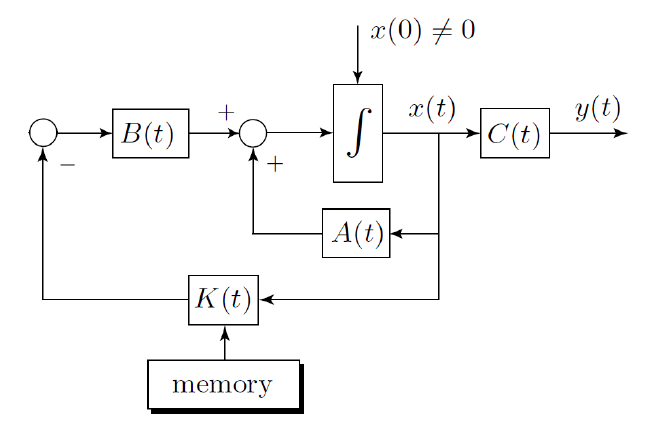
\includegraphics[width=0.65\columnwidth]{finitehor}
\caption{Structure of the finite horizon LQR. }
\label{fig:finitehor}.
\end{figure}

\newpage
\subsubsection{Feedforward LQR Control Systems}
\subsubsection*{Definition}
Referring to Figure \ref{fig:ff}, we can see the structure of the feedforward LQR. The problem is still set up in the interval $[t_a,t_b]$. The objective of the controller is to follow a known reference signal $r(t)$ and to not care how much energy will this cost to us. The feedforward input $u_{ff}(t)$ can be computed in advance as well and stored in another memory. \\
The method to do this, will be explained in the next section. 


\begin{figure}[h]
\centering
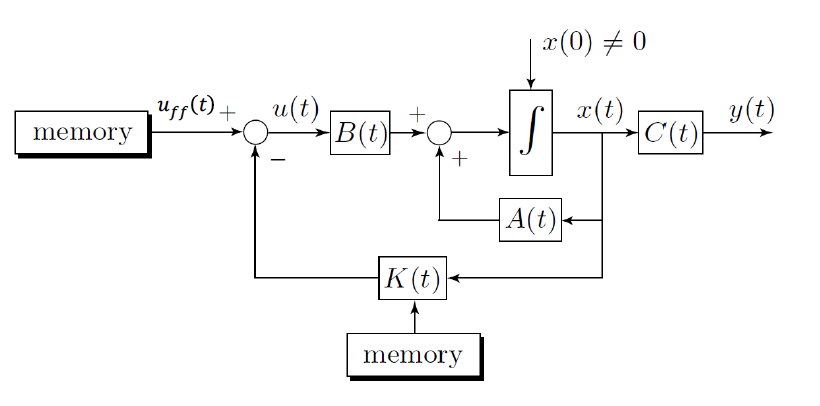
\includegraphics[width=0.75\columnwidth]{ff}
\caption{Structure of the feedforward LQR.}
\label{fig:ff}.
\end{figure}

\newpage

\subsection{Numerical Optimization}
\subsubsection{Definition}
The optimal input 
\begin{equation}
u^*(t\in [0,T])
\end{equation}
is computed numerically offline for the whole planning window  and is used as feedforward signal, i.e. $u_{ff}=u^*(t)$. The numerical optimization is possible, because the planning window has a limited dimension $T$. \\
The criterion we want to minimize is defined as
\begin{equation} \label{numopt}
\begin{split}
\min_{u(t)}J_T(x_0,u(t))&=\min_{u(t)}\int_0^T\underbrace{l(x(t),u(t))}_\text{Stage cost}\,\text{d}t+\underbrace{m(x(t))}_{\text{Terminal cost}} \\
\text{s.t. }  \dot x(t)&=f(t,x(t),u(t)), \\
x(0)&=x_0,\\
x(t)&\in\mathcal{X},u(t)\in\mathcal{U}, \\
x(T)&\in\mathcal{X}_f,
\end{split}
\end{equation}
where 
\begin{itemize}
\item $\dot x(t)=f(t,x(t),u(t))$: Model of the systems;
\item $x(0)=x_0$: Initial Condition;
\item $x(t)\in\mathcal{X},u(t)\in\mathcal{U}$: ``state and input constraint sets'';
\item $x(T)\in\mathcal{X}_f$: ``terminal state constraint set''.
\end{itemize}

\begin{figure}[h]
\centering
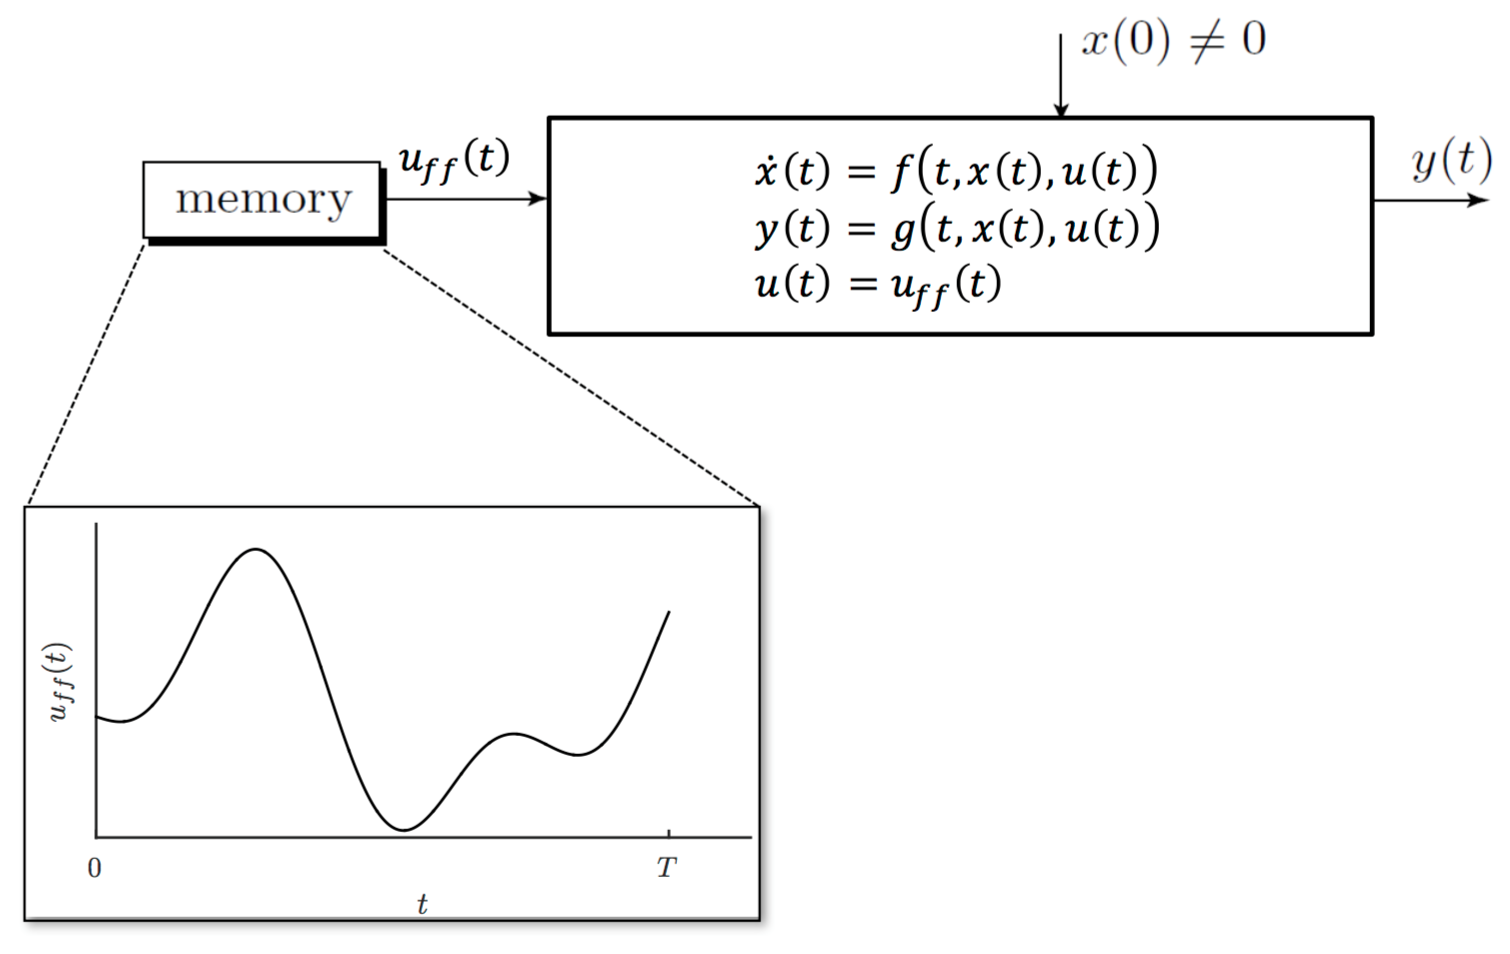
\includegraphics[width=0.7\columnwidth]{numopt}
\caption{Numerical Optimization.}
\end{figure}
\begin{bmk}
A bunch of other courses is offered in order to learn how to approach such an optimization problem. The aim of its introduction in this course, is only that of recognizing the elements thate compose it and understand how the connect to each other.
\end{bmk}
\newpage
\subsubsection{Examples}
\begin{bsp}
You would like to autonomously drive a train from Z\"urich to Lugano without stops in two and a half hours by consuming as little energy as possible. You therefore formulate the optimal control problem as
\begin{equation}
\begin{split}
&\min_{P_m(t\in [0,T])}\int_0^TP_{el}(P_m(t))\text{d}t\\
&\text{s.t.}  \dot s(t)=\sqrt{\frac{2}{m}\cdot E_{kin}(t)}, \\
&\dot{E}_{kin}(t)=P_m(t)-F_{drag}(s(t),E_{kin}(t))\cdot \sqrt{\frac{2}{m}\cdot E_{kin}(t)}, \\
&s(0)=E_{kin}(0)=E_{kin}(T)=0, \ s(T)=S_{end}\\
& |P_m(t)|\leq P_{max}\\
& E_{kin}(t)\leq \frac{m}{2}\cdot v_{max}(s(t))^2,
\end{split}
\end{equation}
where $P_m$ is the power generated by the electric motors, $P_{el}:\mathbb{R}\rightarrow \mathbb{R}$ a nonlinear function describing the relation between mechanical power and power extracted from the electric grid, $s(t)$ is the current position of the train, $E_{kin}(t)$ its current kinetic energy, $F_{drag}(s(t),E_{kin}(t))$ the total drag force, $S_{end}$ the total distance between Z\"urich and Lugano, $P_{max}$ the maximum power that can be exerted by the motors and $v_{max}(s(t))$ the position-dependent maximum speed profile.
\begin{enumerate}[(a)]
\item Identify the state variables $x(t)$ and the input variables $u(t)$.
\item Identify the system dynamics $\dot{x}(t)=f(x(t),u(t))$ and the initial conditions $x_0$. Is it a nonlinear system?
\item What is the stage cost function $l(x(t),u(t))$? Is it linear, quadratic or nonlinear? What about the terminal cost function $m(x(T))$ and the objective function $J_T(x_0,u(t))$?
\item What is the value of $T$ in seconds?
\item Identify the state, input and terminal state constraint sets $\mathcal{X}, \mathcal{U}, \mathcal{X}_f$.
\end{enumerate}

\newpage
\begin{lsg}
\
\begin{enumerate}[(a)]
\item The state variabes are easy to see: they are the train position and the its kinetic energy. The state vector reads
\begin{equation*}
x(t)=\begin{pmatrix} s(t)\\E_{kin}(t) \end{pmatrix}.
\end{equation*}
We are given only an input: the power exerted by the motors. Mathematically:
\begin{equation*}
u(t)=P_m(t).
\end{equation*}
\item The system dynamics are computed by taking the derivative of the state vector. Reading from the problem's description one gets
\begin{equation*}
\dot{x}(t)=\begin{pmatrix} 
\sqrt{\frac{2}{m}\cdot x_2(t)} \\[6pt]
u(t)-F_{drag}(x_1(t),x_2(t))\cdot \sqrt{\frac{2}{m}\cdot x_2(t)}
\end{pmatrix},
\end{equation*}
with $x_1(t)$, $x_2(t)$ state variables. Of course, this represents a nonlinear dynamical system. The initial conditions are $x_0=0$.
\item The stage cost function is $$l(x(t),u(t))=P_{el}(u(t))$$ and is nonlinear.\\ The terminal cost function is zero, i.e.
\begin{equation*}
m(x(T))=0.
\end{equation*}
The objective function reads
\begin{equation*}
J_T(x_0,u(t))=\int_0^{T}P_{el}(u(t))\text{d}t.
\end{equation*}
\item Since we would like to complete our journey within 2.5 hours, it holds
$$T=3600s/h\cdot 2.5h=9000s.$$
\item The state constraint set is 
\begin{equation*}
\mathcal{X}=\{x\in \mathbb{R}^2: 0\leq x_1\leq S_{end},\ x_2\leq \frac{m}{2}\cdot v^2_{max}(x_1)\}.
\end{equation*}
The input constraint set is
\begin{equation*}
\mathcal{U}=\{u\in \mathbb{R}: |u|\leq P_{max}\}.
\end{equation*}
The terminal state constraint set is
\begin{equation*}
\mathcal{X}_f=\{\begin{pmatrix} S_{end}\\ 0 \end{pmatrix} \}.
\end{equation*}




\end{enumerate}

\end{lsg}

\end{bsp}

\newpage

\subsection{Model Predictive Control (MPC)}
A whole course about this topic is offered in the master at IDSC (Prof. Zeilinger). 
\subsubsection{Definition}
Basically, with MPC one solves in each time step the numerical optimization problem defined in the previous section. The solution is always given as feedback to the system. 
\subsubsection*{Method}
For every $\Delta t$ this procedure is applied:
\begin{enumerate}[(I)]
\item Measure or estimate the actual state, i.e.
\begin{equation}
x(t)=z.
\end{equation}
\item Find the optimal input for the whole planning window $T$:
\begin{equation}
u^*([0,T])=\text{arg}\min_{u([0,T])}J_T(z,u([0,T])),
\end{equation}
with the model and the constraints introduced in \ref{numopt}.
\begin{bmk}
$\text{arg}\min f(x)$ is the argument that minimizes $f(x)$.
\end{bmk}

\item Implement just the first part 
\begin{equation}
u^*([0,\Delta t])
\end{equation}
of the calculated solution.
\end{enumerate}

\begin{figure}[h]
\centering
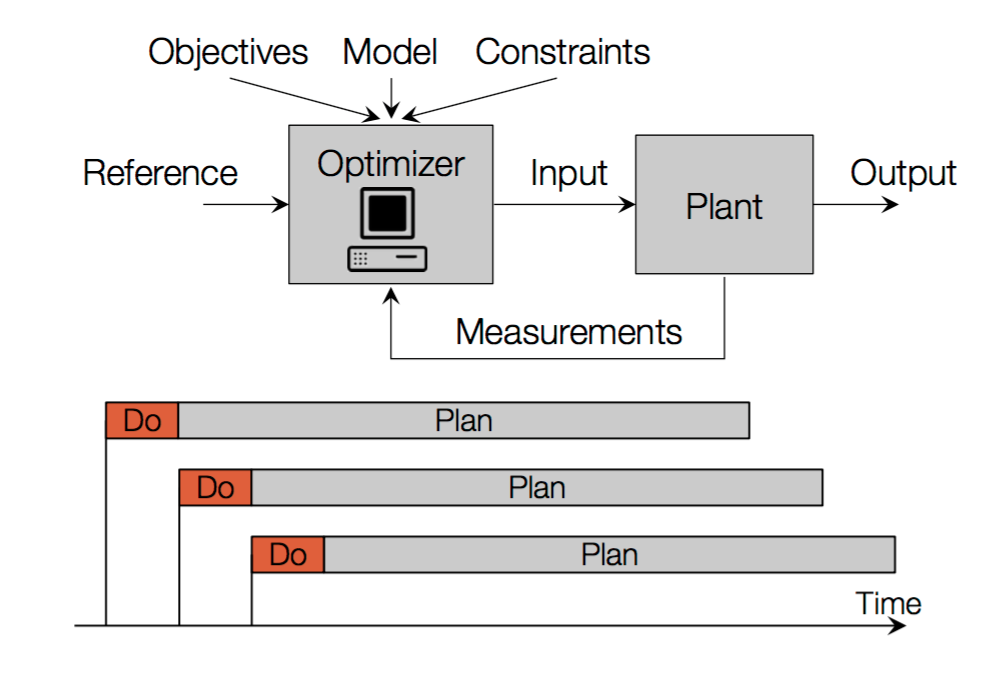
\includegraphics[width=0.75\columnwidth]{mpc}
\caption{MPC method description.}
\label{fig:mpc}.
\end{figure}
One of the big advantages of Model Predictive Control, is that this method can work with every model, i.e. also with nonlinear models and delay elements. Another advantage is that the criterion (objective function) can be freely chosen. However, stability is not guaranteed and good models are computationally demanding.

\subsubsection{Examples}
\begin{bsp}
Consider the Model Predictive Control scheme $\mathcal{P}(x_0)$
\begin{equation*}
\begin{split}
&\min_{u(t\in [0,T])}\int_0^T q\cdot x^2(t)+r\cdot u^2(t)\text{d}t\\
&\text{s.t.} \ \dot{x}(t)=u(t),\ x(0)=x_0\\
&u(t)\in \mathcal{U},\ x(t)\in \mathcal{X},\ x(T)\in \mathcal{X}_f.
\end{split}
\end{equation*}
\begin{enumerate}[(a)]
\item How can we solve the problem for $T\rightarrow \infty$ and $\mathcal{X}=\mathcal{U}=\mathcal{X}_f=\mathbb{R}$? What is the solution for $u^*(t)$?
\item What happens if the value of $r$ is decreased? And what if it is increased? Inlcue the notion of \textit{cheap} and \textit{expensive} control in your reasoning.
\item In this case would you need to iteratively solve the optimization problem? Why?
\item Consider now a finite horizon $T$ and the constraint sets
\begin{equation*}
\begin{split}
\mathcal{X}&=\mathbb{R}\\
\mathcal{U}&=\{ u\in \mathbb{R}: |u|\leq u_{max}\}\\
\mathcal{X}_f&=\{ 0\}.
\end{split}
\end{equation*}
Define the feasible set of this MPC scheme, i.e. find the set
\begin{equation*}
\mathcal{X}_T=\{ x_0\in \mathbb{R}:\mathcal{P}(x_0) \text{ admits a feasible solution}\}.
\end{equation*}
What happens if $x_0 \not \in \mathcal{X}_T$?
\item Now also consider 
\begin{equation*}
\mathcal{X}=\{x \in \mathbb{R}:0\leq x \leq x_{max} \}.
\end{equation*}
How does the $\mathcal{X}_T$ change?
\end{enumerate}
\newpage
\begin{lsg}
\
\begin{enumerate}[(a)]
\item The MPC optimization problem becomes
\begin{equation*}
\min_{u(t)}\int_0^\infty q\cdot x^2(t)+r\cdot u^2(t)\text{d}t\\
\text{s.t. } \dot{x}(t)=u(t),\ x(0)=x_0. 
\end{equation*}
This is a classic unconstrained infinite-horizon LQR problem that we can tackle solving the scalar version of the Continuous-time Algebraic Riccati Equation (CARE):
\begin{equation*}
\frac{1}{r}\cdot B^2 \cdot \Phi^2-2\cdot A\cdot \Phi -q=0.
\end{equation*}
Since in our case
\begin{equation*}
\begin{split}
A&=0\\
B&=1\\
\end{split}
\end{equation*}
and $\Phi>0$, we obtain
\begin{equation*}
\Phi=\sqrt{q\cdot r}.
\end{equation*}
Therefore, the static gain for the optimal state-feedback regulator is 
\begin{equation*}
\begin{split}
K&=\frac{B}{r}\cdot \Phi\\
&=\sqrt{\frac{q}{r}}.
\end{split}
\end{equation*}
We know that 
\begin{equation*}
u^*(t)=-K\cdot x(t),
\end{equation*}
where $x(t)$ can be computed from the dynamics of the closed loop
\begin{equation*}
\dot{x}(t)=-K\cdot x(t).
\end{equation*}
This is an easy differential equation and the solution reads
\begin{equation*}
\begin{split}
x^*(t)&=x_0\cdot e^{-K\cdot t}\\
&=x_0\cdot e^{-\sqrt{\frac{q}{r}}\cdot t}.
\end{split}
\end{equation*}
Plugging this into the wanted input we find
\begin{equation*}
\begin{split}
u^*(t)&=-K\cdot x^*(t)\\
&=-\sqrt{\frac{q}{r}}\cdot x_0 \cdot e^{-\sqrt{\frac{q}{r}}\cdot t}.
\end{split}
\end{equation*}
\item This case is interesting to analyze, since the control gain $K$ is the same as the convergence rate of the state variable. If the value of $r$ is decreased we would do cheap control: the \textit{cheaper} control energy would result in a fastest convergence rate $K=\sqrt{\frac{q}{r}}$ at the expense of a larger control gain. If we increase $r$, making the control enery more \textit{expensive}, the control gain will be reduced at the expensive of a slower convergence rate.
\item It is not necessary to solve the optimization problem iteratively, as for this special case the optimal input $u^*(t)$ can be computed as a closed form solution. Typically, this would not be possible, as the presence of state and input contraints would not allow to solve the optimization problem analytically. In that case, a numerical solver must be employed.
\item The state dynamics are given by the open integrator $\dot{x}(t)=u(t)$. Hence the maximum change achievable in $x$ over the ifnite horizon $T$ can be computed integrating the minimum and maximum values allowed for the input, i.e. $u(t)=\pm u_{max}$. Since the input constraint is symmetric, we obtain for the maximum achievable distance for both negative and positive directions
\begin{equation*}
\Delta x_{max}=\int_0^T u_{max} \text{d}t=u_{max} \cdot T.
\end{equation*}
As we do not have state constraints, but we are only forcing the state variable to be at the origin at the end of the horizon, i.e. $$x(T)\in \mathcal{X}_f=\{0\}\Rightarrow x(T)=0,$$ the feasible set is defined by all the initial conditions whose distance from the origin is less than the maxmum achievable distance $\Delta x_{max}$, i.e.
\begin{equation*}
\begin{split}
\mathcal{X}_T&=\{x_0\in \mathbb{R}: \mathcal{P}(x_0) \text{ admits a feasible solution}\\
&=\{ x_0 \in \mathbb{R}: |x_0|\leq u_{max}\cdot T\}.
\end{split}
\end{equation*}
If at some point $x_0 \not \in \mathcal{X}_T$, which means $|x_0|>\Delta x_{max}$, there will be no admissible control trajectory able to steer the state variable to the origin within the horizon $T$, and therefore the MPC problem will be unfeasible and no solution will be found.
\item Since we are now imposing the addition contraint 
\begin{equation*}
x(t)\in \mathcal{X}=\{x\in \mathbb{R}:0\leq x \leq x_{max}\},
\end{equation*}
$x_0$ must always be inside of $\mathcal{X}$. Hence, $\mathcal{X}_T$ results from the intersection of the admissible set computed in part (c) $\mathcal{X}_T^{\text{old}}$ and the state constraint set $\mathcal{X}$ as
\begin{equation*}
\mathcal{X}_T^\text{old}\cap \mathcal{X}=\{x_0\in \mathbb{R}:0\leq x_0 \leq \min\{u_{max}\cdot T,x_{max}\}.
\end{equation*}








\end{enumerate}

\end{lsg}


\end{bsp}
\newpage
\subsection{The Linear Quadratic Gaussian (LQG)}
In the previous section we assumed that all the state variables of the system were given. In non academic cases, however, this is not the case: one knows just the output $y(t)$ and the input $u(t)$. Hence, one has to figure out how to get the actual state $x(t)$. The idea is to use an \textbf{observer} to get an estimate of $x(t)$, also called $\hat{x}(t)$. A whole course about estimation if offered at IDSC in the master by Prof. D'Andrea: \textit{Recursive Estimation}.
\subsubsection{Observer}
For the following explanations, I refer to Figure \ref{fig:lqg}. The idea is to \textit{copy} the internal description of the plant and its dynamics, in order to predict $\hat{x}(t)$. This is done by connecting two feedback loops through the observer gain $L$, that can be tuned for different applications. First of all, let's define the observation error as
\begin{equation}
\bar{x}(t)=x(t)-\hat{x}(t) \ \in \mathbb{R}^n.
\end{equation}
The dynamics of the error are described by its derivative, namely
\begin{equation}
\begin{split}
\frac{\text{d}}{\text{d}t}\bar{x}(t)&=\frac{\text{d}}{\text{d}t}x(t)-\frac{\text{d}}{\text{d}t}\hat x(t) \\
&=A\cdot x(t)+B\cdot u(t)-(\hat A\cdot\hat x(t)+\hat B\cdot u(t)+L\cdot (C\cdot x(t)-\hat C\cdot\hat x(t))) \\
&=A\cdot \bar x(t)-L\cdot C\cdot \bar x(t) \\
&=(A-L\cdot C)\cdot \bar x(t),
\end{split}
\end{equation}
by assuming the \textbf{exact} duplication of the system's dynamics, i.e. $A=\hat{A}$, $B=\hat{B}$ and $C=\hat{C}$. If the matrix $A-L\cdot C$ has \textbf{asymptotically stable} eigenvalues, the observation error will converge asymptotically to 0. The speed of convergence can be \textit{tuned} with the gain $L$. \\
The whole point here, is to find such a matrix with asymptotically stable eigenvalues. Since with the LQR approach we are guaranteed to have asymptotically stable eigenvalues for the matrix $A-B\cdot K$, we can find similarities between the two: in fact the roles of $B$ and $C$ are interchanged. By converting the problem, in order to get the same role for the matrices, one gets
\begin{equation}
A-L\cdot C \Rightarrow (A-L\cdot C)^T=A^T-C^T\cdot L^T
\end{equation}
This makes the things easier: we can now, according to Table \ref{table:LQG}, approach this problem as a LQR problem with changed matrices.
By plugging the new matrices into the Riccati equation, one gets
\begin{equation}
\frac{1}{q}\cdot \Psi\cdot C^\intercal\cdot C\cdot \Psi-\Psi\cdot A^\intercal-A\cdot\Psi-\bar B\cdot \bar B^\intercal=0,
\end{equation}
where $\Psi$ is its solution. The matrix $L$ is then given as
\begin{equation}
L^\intercal=\frac{1}{q}\cdot C\cdot\Psi.
\end{equation}
\newpage
\begin{table}
\begin{center}\begin{tabular}{c|c} \toprule
LQR & LQG \\ \midrule
$[A-B\cdot K]$  & $[(A-L\cdot C)^\intercal]=[(A^\intercal-C^\intercal\cdot L^\intercal)]$ \\
$A$ & $A^\intercal$ \\
$B$ & $C^\intercal$ \\
$Q=\bar C^\intercal\cdot \bar C$  & $\bar B\cdot\bar B^\intercal$ \\
$R=r\cdot \mathbb{1}$  & $q\cdot \mathbb{1}$ \\ \bottomrule
\end{tabular}\end{center}
\caption{LQG and LQR.}
\label{table:LQG}
\end{table}


\begin{figure}[h]
\centering
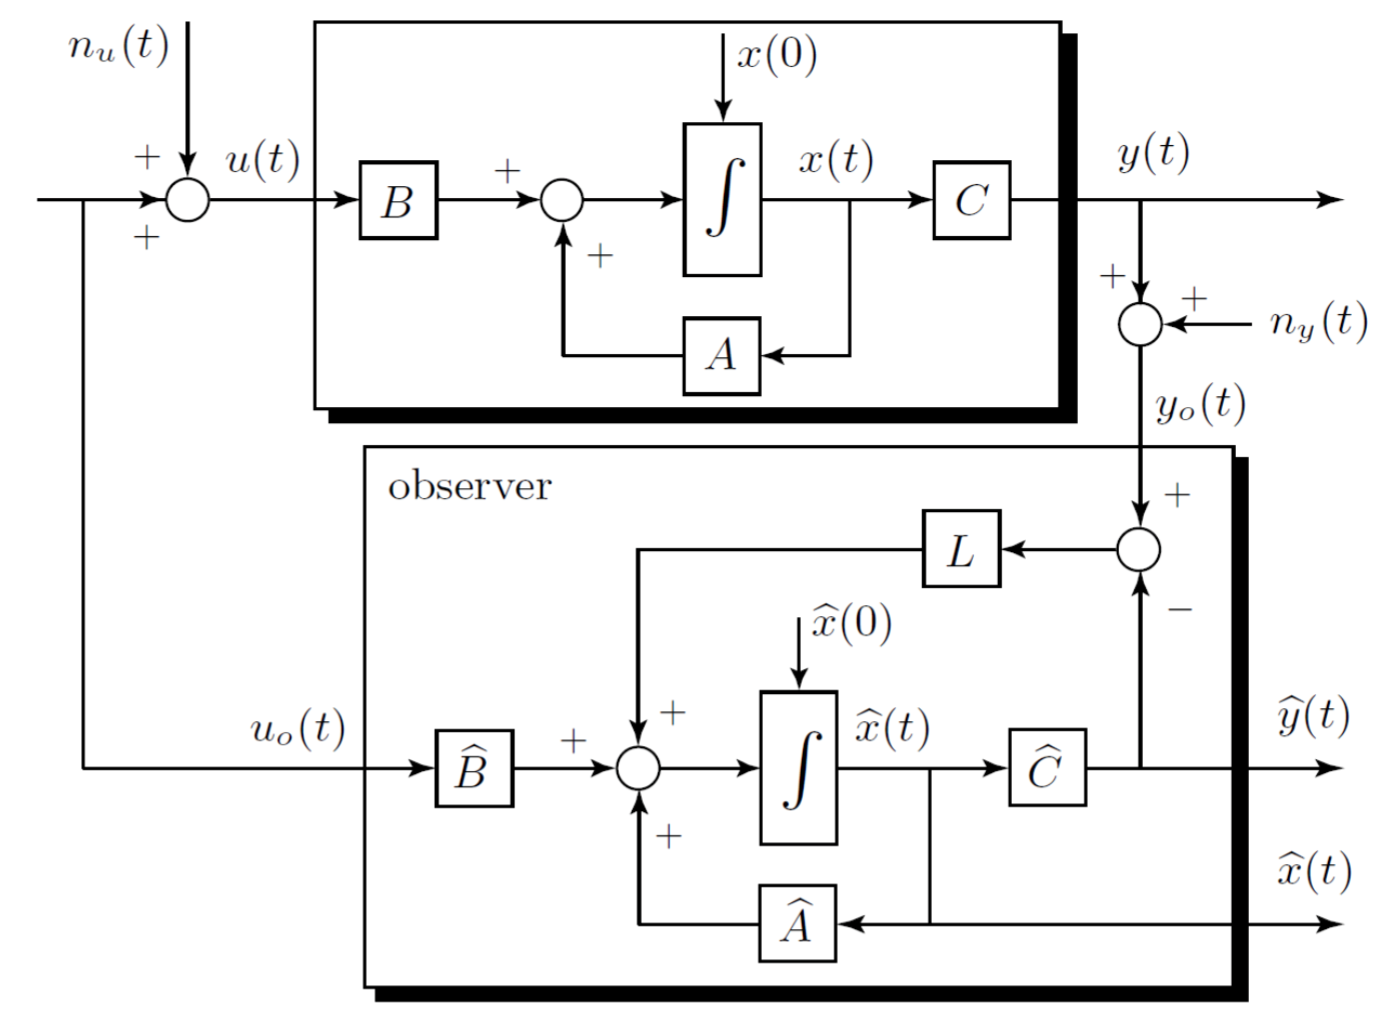
\includegraphics[width=0.6\columnwidth]{lqg}
\caption{Structure of a state observer.}
\label{fig:lqg}.
\end{figure}


\subsubsection{The LQG Controller}
The LQG controller uses the LQR approach and the concept of the observer and connect the two into a unique system. Starting from the solution of the LQR problem, that contained the controller $K$ and the observed signal $\hat{x}(t)$ from the observer, one can write as learned
\begin{equation}
u(t)=-K\cdot \hat{x}(t).
\end{equation}
Since we have now an estimate of $x(t)$, we can approach the problem with a normal LQR method. Let's define
\begin{equation}
\tilde{x}=\begin{pmatrix} x(t) \\ \hat{x}(t)\end{pmatrix}.
\end{equation}
By connecting the observer and the plant with the gain $-K$ one can actually analyze the open loop and the closed loop system conditions:
\subsubsection*{Open Loop Conditions}
For open loop conditions, we can write the state dynamics as
\begin{equation}
\frac{\text{d}}{\text{d}t}\tilde{x}(t)=\tilde{A}_{\text{open loop}}\cdot \tilde{x}(t)+\tilde{B}_{\text{open loop}}\cdot e(t).
\end{equation}
By looking at Figure \ref{fig:lqg2}, we can derive
\begin{equation}
\begin{split}
\tilde{A}_{\text{open loop}}&=\begin{pmatrix}
A&-B\cdot K\\
0&A-B\cdot K -L\cdot C
\end{pmatrix},\\
\tilde{B}_{\text{open loop}}&=\begin{pmatrix}
0\\
-L
\end{pmatrix},\\
\tilde{C}_{\text{open loop}}&=\begin{pmatrix}
C&0
\end{pmatrix}.
\end{split}
\end{equation}
\subsubsection*{Closed Loop Conditions}
For closed loop conditions, we can write the state dynamics as
\begin{equation}
\frac{\text{d}}{\text{d}t}\tilde{x}(t)=\tilde{A}_{\text{closed loop}}\cdot \tilde{x}(t)+\tilde{B}_{\text{closed loop}}\cdot e(t)
\end{equation}
and analogously it follows from Figure \ref{fig:lqg2} that
\begin{equation}
\begin{split}
\tilde{A}_{\text{closed loop}}&=\begin{pmatrix}
A&-B\cdot K\\
L\cdot C&A-B\cdot K -L\cdot C
\end{pmatrix},\\
\tilde{B}_{\text{closed loop}}&=\begin{pmatrix}
0\\
-L
\end{pmatrix},\\
\tilde{C}_{\text{closed loop}}&=\begin{pmatrix}
C&0
\end{pmatrix}.
\end{split}
\end{equation}
If one analyzes this in the frequency domain, one gets
\begin{equation}
\begin{split}
L_{\text{LQG}}(s)&=P(s)\cdot C(s)\\
&=\underbrace{C\cdot \left( s\cdot \mathbb{1}-A\right))^{-1}\cdot B}_{P(s)}\cdot \underbrace{K\cdot \left( s\cdot \mathbb{1} -(A-B\cdot K-L\cdot C)\right)^{-1}\cdot L}_{C(s)}
\end{split}
\end{equation}
and
\begin{equation}
T_{\text{LQG}}(s)=L_{\text{LQG}}(s)\cdot (\mathbb{1}+L_{\text{LQG}}(s))^{-1}.
\end{equation}
\begin{bmk}
\
\begin{itemize}
\item If the LQ regulator and the observer are stable, then so is the LQG closed loop.
\item If the LQ regulator and the observer are robust, nothing can be said about the robustness of the LQG closed loop. This means that we don't habe guarantee on robustness and it must be investigated a posteriori.
\end{itemize}

\end{bmk}

\subsubsection{Kochrezept}
\begin{enumerate}[(I)]
\item Find $K$: Solve a standard LQR problem with
\begin{equation}
\{A,B,Q=\bar{C}^T\cdot \bar{C},R\}
\end{equation}
\item Find $L$: Solve a standard LQR problem with
\begin{equation}
\{A^T,C^T,Q=\bar{B}\cdot \bar{B},R=q\cdot \mathbb{1}\}
\end{equation}
\item Use the \textsc{Matlab} command
\begin{verbatim}
K=lqr(A,B,C_tilde'*C_tilde,r*eye(m,m)),L=lqr(A',C',B_bar*B_bar',q*eye(p,p))'.
\end{verbatim}
\begin{bmk}
It must hold
\begin{itemize}
\item $\{ A,C\}$ completely observable
\item $\{A,\bar{B}\}$ completely controllable.
\end{itemize}
\end{bmk}

\end{enumerate}








\begin{figure}[h]
\centering
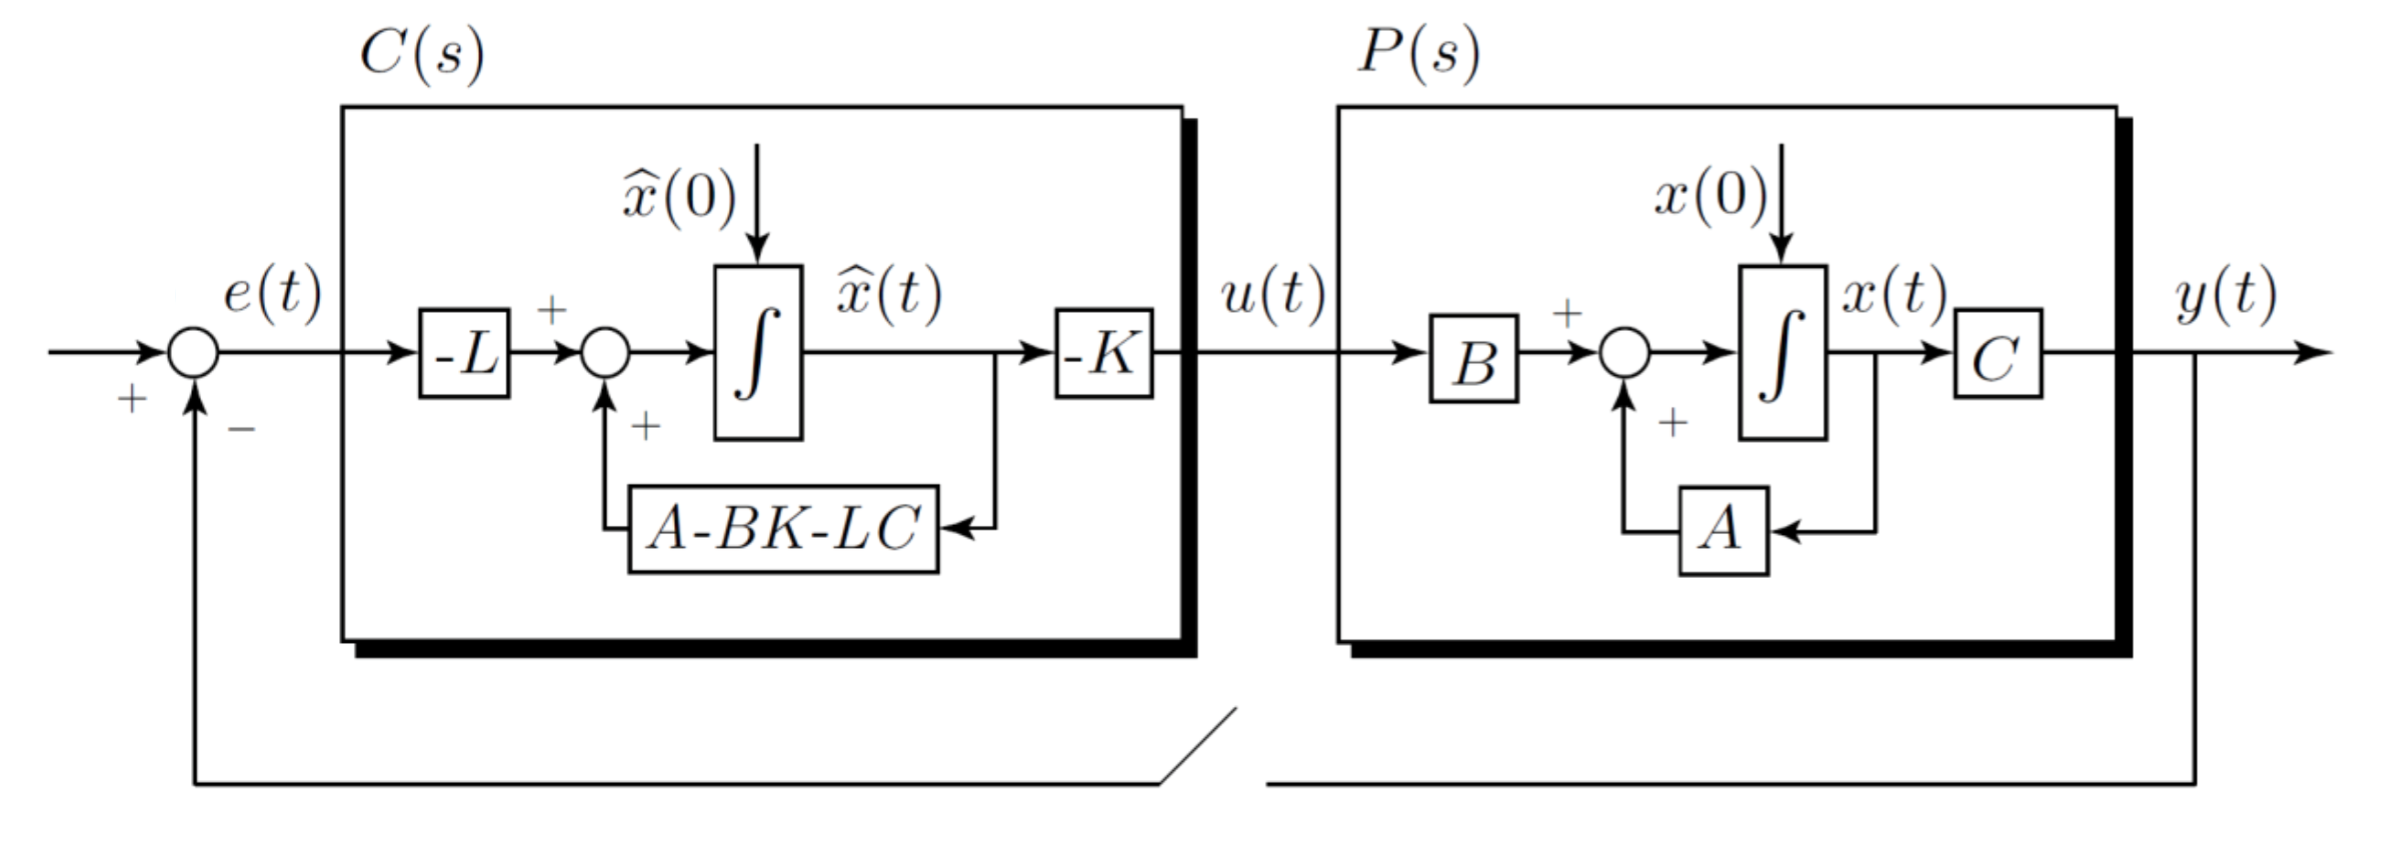
\includegraphics[width=\columnwidth]{lqg2}
\caption{Structure of LQG controller.}
\label{fig:lqg2}.
\end{figure}


\newpage

\subsubsection{Examples}
\begin{bsp}
The dynamics of a system are given as
\begin{equation*}
\begin{split}
\dot{x}_1(t)&=x_2(t)\\
\dot{x}_2(t)&=u(t)\\
y(t)&=x_1(t).
\end{split}
\end{equation*}
You want to design a state observer. The observer should use the measurements for $y(t)$ and $u(t)$ in order to estimate the state variables $\hat{x}(t)\sim x(t)$.
\begin{enumerate}[(a)]
\item Which dimension has the observer matrix $L$? Draw the signal diagram of such an observer.
\item Compute the observer matrix $L$ for $q=1$.
\item You have already computed a state feedback matrix $K=\begin{pmatrix} 1&1 \end{pmatrix}$ for the system above. What is the complete transfer function of the controller $C(s)$? Use $L=\begin{pmatrix} \sqrt{2} \\ 1 \end{pmatrix}$.
\end{enumerate}

\newpage
\begin{lsg}
\
\begin{enumerate}[(a)]
\item Since $C$ is a $1\times 2$ matrix and $L\cdot C$is of the same dimensions of $A$, $2\times 2$ matrix, $L$ is a $2 \times 1$ matrix, i.e.
\begin{equation*}
L=\begin{pmatrix} L_1 \\ L_2 \end{pmatrix}.
\end{equation*}
By adapting the general structure of an observer one gets Figure \ref{fig:lqg3}.

\begin{figure}[h]
\centering
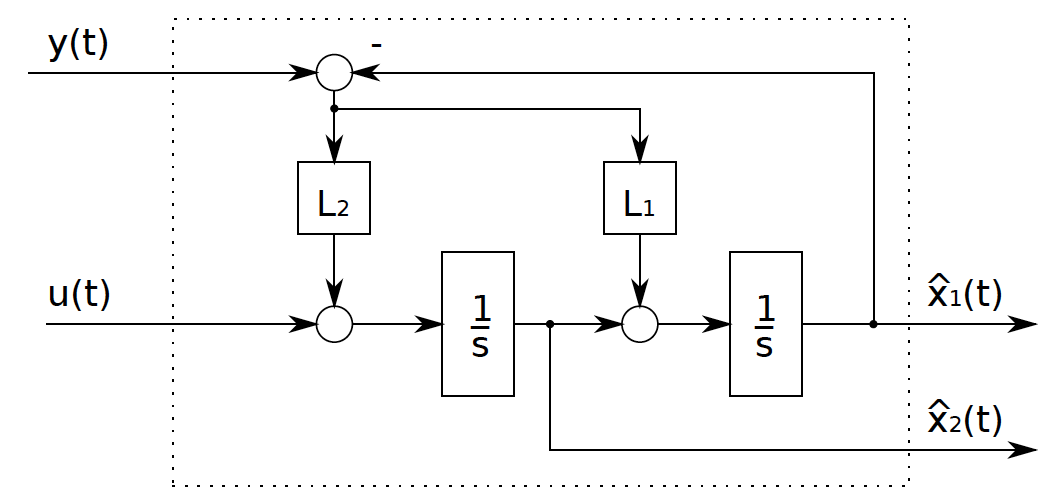
\includegraphics[width=0.6\columnwidth]{lqg3}
\caption{Structure of the state observer.}
\label{fig:lqg3}.
\end{figure}

\item First of all let's read the system matrices:
\begin{equation*}
\begin{split}
A&=\begin{pmatrix}
0&1\\ 0&0
\end{pmatrix}\\
B&=\begin{pmatrix}
0\\ 1\end{pmatrix}\\
C&=\begin{pmatrix} 1&0 \end{pmatrix} \\
D&=0.
\end{split}
\end{equation*}
Plugging these matrices into the Riccati equation one gets:
\begin{equation*}
\begin{split}
\frac{1}{q}\cdot \Psi \cdot C^T \cdot C \cdot \Psi - \Psi \cdot A^T -A\cdot \Psi - B\cdot B^T&=0\\
\Psi \cdot \begin{pmatrix} 1\\ 0\end{pmatrix}\cdot \begin{pmatrix} 1&0 \end{pmatrix} \cdot \Psi- \Psi \cdot \begin{pmatrix}
0&1\\ 0&0
\end{pmatrix}-\begin{pmatrix}
0&0\\ 1&0
\end{pmatrix}\cdot \Psi-\begin{pmatrix} 1\\ 0\end{pmatrix}\cdot \begin{pmatrix} 0&1\end{pmatrix}&=\begin{pmatrix} 0&0\\ 0&0 \end{pmatrix}\\
\begin{pmatrix}
\psi_1^2& \psi_1\cdot \psi_2 \\
\psi_1\cdot \psi_2 & \psi_2^2
\end{pmatrix}-\begin{pmatrix}
2\psi_2 & \psi_3 \\
\psi_3 &0
\end{pmatrix}-\begin{pmatrix}
0&0\\ 0&1
\end{pmatrix}&=\begin{pmatrix}
0&0\\ 0&0 
\end{pmatrix}.
\end{split}
\end{equation*}
The matrix $\Psi$ is symmetric and positive definite and with these informations we can compute its elements:
\begin{itemize}
\item From the last term of the equation one gets
\begin{equation*}
\psi_2^2=1 \Rightarrow \psi_2=\pm 1.
\end{equation*}
\item By plugging this into the first equation one gets $\psi_1=\pm \sqrt{2}$. Because the positive definite condition, one gets $\psi_1=\sqrt{2}$, $\psi_2=1$.
\item Because of the form of $C$ we don't care about $\psi_3$.
\end{itemize}
From these calculations it follows
\begin{equation*}
\begin{split}
L^T&=\frac{1}{q}\cdot C \cdot \Psi\\
&=\frac{1}{1}\cdot \begin{pmatrix} 1&0 \end{pmatrix} \cdot \begin{pmatrix}
\sqrt{2}&1\\
1&*
\end{pmatrix}\\
&=\begin{pmatrix}
\sqrt{2}&1
\end{pmatrix},
\end{split}
\end{equation*}
and so
\begin{equation*}
L=\begin{pmatrix} \sqrt{2}\\ 1\end{pmatrix}.
\end{equation*}
\item As it is shown in the theory, the formula to calculate the controller's transfer function reads
\begin{equation*}
C(s)=K\cdot (s\cdot \mathbb{1}-(A-B\cdot K -L\cdot C))^{-1}\cdot L.
\end{equation*}
By plugging in the found matrices one gets
\begin{equation*}
\begin{split}
(A-B\cdot K-L\cdot C)&=\begin{pmatrix}
0&1\\ 0&0 \end{pmatrix} -\begin{pmatrix} 0\\ 1 
\end{pmatrix}\cdot \begin{pmatrix} 1&1 \end{pmatrix} -\begin{pmatrix} \sqrt{2}\\ 1 \end{pmatrix} \cdot \begin{pmatrix} 1&0\end{pmatrix}\\
&=\begin{pmatrix}
0&1\\ 0&0 \end{pmatrix}- \begin{pmatrix} 
 0&0\\ 1&1
 \end{pmatrix}-\begin{pmatrix}
\sqrt{2}&0\\ 1 & 0 
\end{pmatrix}\\
&=\begin{pmatrix}
-\sqrt{2}&1\\
-2&-1
\end{pmatrix}.
\end{split}
\end{equation*}
It follows
\begin{equation*}
\begin{split}
(s\cdot \mathbb{1}-(A-B\cdot K -L\cdot C))^{-1}&=\begin{pmatrix}
s+\sqrt{2} & -1\\
2&s+1
\end{pmatrix}^{-1}\\
&=\frac{1}{(s+\sqrt{2})\cdot (s+1) +2}\cdot \begin{pmatrix}
s+1 & 1\\
-2&s+\sqrt{2}
\end{pmatrix}.
\end{split}
\end{equation*}
By plugging this into the formula one gets
\begin{equation*}
\begin{split}
C(s)&=K\cdot (s\cdot \mathbb{1}-(A-B\cdot K -L\cdot C))^{-1}\cdot L\\
&=\begin{pmatrix} 1&1 \end{pmatrix}\cdot \frac{1}{(s+\sqrt{2})\cdot (s+1) +2}\cdot \begin{pmatrix}
s+1 & 1\\
-2&s+\sqrt{2}
\end{pmatrix}\cdot \begin{pmatrix} \sqrt{2}\\ 1\end{pmatrix}\\
&=\frac{1}{(s+\sqrt{2})\cdot (s+1) +2}\cdot \begin{pmatrix}
s-1&s+1+\sqrt{2}
 \end{pmatrix}\cdot \begin{pmatrix} \sqrt{2}\\ 1\end{pmatrix}\\
&=\frac{1}{(s+\sqrt{2})\cdot (s+1) +2}\cdot (\sqrt{2}s-\sqrt{2}+s+1+\sqrt{2})\\
&=\frac{(\sqrt{2}+1)s+1}{(s+\sqrt{2})\cdot (s+1) +2}.
\end{split}
\end{equation*}
\end{enumerate}
\end{lsg}
\end{bsp}


\newpage
\begin{bsp}
You are working for your semester thesis at a project which includes a water reservoir. Your task is to determine the disturbance $d(t)$ that acts on the reservoir. Figure \ref{res_1} shows the situation. The only state of the system is the water volume $x(t)=V(t)$. The volume flows in the reservoir $V_{\text{in}}^*(t)$ are the known system input $u(t)$ and the unknown disturbance $d(t)>0$. The volume flow of the system is assumed to be only dependend on the water volume, i.e.
\begin{equation*}
V_{\text{out}}^*(t)=-\beta \cdot x(t).
\end{equation*}
The system output $y(t)$ is the water level $h(t)$. The model of this reservoir reads
\begin{equation}
\begin{split}
\frac{\text{d}x(t)}{\text{d}t}&=-\beta \cdot x(t) + u(t) + d(t),\\
y(t)&= \frac{1}{\alpha} \cdot x(t), \ \alpha>0, \ \beta>0.
\end{split}
\end{equation}




\begin{figure}[h!]
\centering
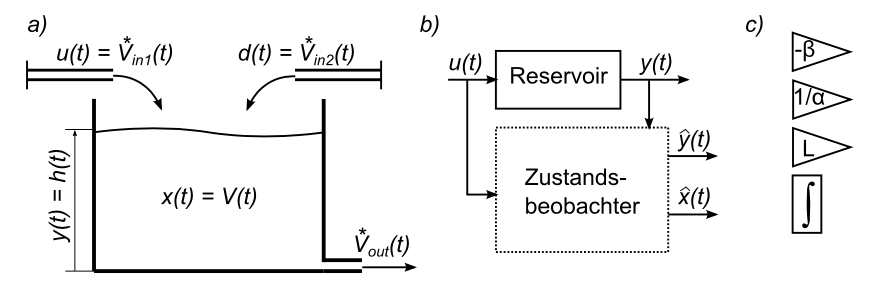
\includegraphics[width=0.75\columnwidth]{reservoir}
\caption{a) Drawing of the reservoir; b) Inputs and Outputs of the observer; c) Blocks for signal flow diagram.}
\label{fig:res_1}.
\end{figure}
The goal is to determine $d(t)$. Your supervisor has already tried to solve the model equations for $d(t)$: he couldn't determine the change in volume  $\frac{\text{d}x(t)}{\text{d}t}$ with enough precision. Hence, you want to solve this problem with a state observer.
\begin{enumerate}[(a)]
\item Draw the signal flow diagram of such a state observer. Use the blocks of Figure \ref{res_1}c).
\item The state feedback matrix $L$ is in this case some scalar value. Which value can $L$ be, in order to get an asymptotically stable state observer?
\item Introduce a new signal $\hat{d}(t)$ in the state observer. This should approximate the real disturbance $d(t)$.
\item Find the state space description of the observer with inputs $u(t)$ and $y(t)$ and output $\hat{d}(t)$.
\end{enumerate}

\newpage


\begin{lsg}
\
\begin{enumerate}[(a)]
\item The signal flow diagram can be seen in Figure \ref{fig:res_2}.
\begin{figure}[h!]
\centering
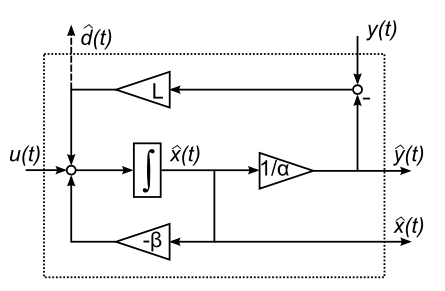
\includegraphics[width=0.75\columnwidth]{reserv}
\caption{Signal flow diagram of the state observer.}
\label{fig:res_2}.
\end{figure}
\item The stability of the ovserver depends on the eigenvalues of $A-L\cdot C$. In this case, since $A-L\cdot C $ is a scalar, $$A-L\cdot C<0$$ should hold. This leads to $$L>\frac{A}{C}$$. With the given informations it follows
$$L>-\frac{\beta}{\alpha}.$$
\item The dashed line in Figure \ref{fig:res_2} represents the new output $\hat{d}(t)$. The integrator in Figure \ref{fig:res_2} has now 3 inputs. The arrow from downwards from the reservoir is $V_{\text{out}}^*(t)$, the arrow from left is the input flow $u(t)=V_{\text{in1}}^*(t)$. If we simulate the system without the dashed arrow, there is a deviation between the measured $y(t)$ and the simulated $\hat{y}(t)$. This results from the extra inflow $d(t)=V_{\text{in}}^*(t)$, which is not considered in the simulation. 
\item The new state-space description reads
\begin{align*}
\frac{\text{d}\hat{x}(t)}{\text{d}t}&= \left(-\beta -\frac{L}{\alpha}\right)\cdot \hat{x}(t)+ (1)\cdot u(t) +(L)\cdot y(t)\\
\hat{d}(t)&=\left( -\frac{L}{\alpha}\right) \cdot \hat{x}(t)+(0)\cdot u(t)+(L)\cdot y(t).
\end{align*}
 
\end{enumerate}

\end{lsg}

\end{bsp}


\subsection{Extension of LQG}
\subsubsection{The LQGI}
As for the LQR the LQRI problem can be introduced, one can introduce a LQGI as well. The concept is really similar and the new matrices to compute are $K$ ,$K_I$ and $L$.
Please refer for the following computations to Figure \ref{fig:lqgi}.

\subsubsection*{Kochrezept}
\begin{enumerate}[(I)]
\item Find $K$ and $K_I$ by solving a standard LQR problem (see LQRI) with 
\begin{equation}
\{ \tilde{A},\tilde{B},\tilde{C},\tilde{D}\}
\end{equation}
\item Find $L$ by solving a standard LQR problem with
\begin{equation}
\{ \tilde{A}^T,\tilde{C}^T,Q=\bar{B}\cdot \bar{B}^T,R=q\cdot \mathbb{1}\}
\end{equation}
\end{enumerate}
This can be one more time analyzed with open loop and closed loop conditions:
\subsubsection*{Open Loop Conditions}
The state space description for open loop conditions reads
\begin{equation}
\begin{split}
\frac{\text{d}}{\text{d}t}\begin{pmatrix}
x(t)\\
\hat{x}(t)\\
v(t)
\end{pmatrix}&=\begin{pmatrix}
A & -B_u\cdot K & B_u\cdot K_I\\
0&A-B_u\cdot K-L\cdot C & B_u\cdot K_I\\
0&0&0
\end{pmatrix}\cdot 
\begin{pmatrix}
x(t)\\
\hat{x}(t)\\
v(t)
\end{pmatrix} +\begin{pmatrix}
0\\ -L \\ \mathbb{1}
\end{pmatrix}\cdot e(t)\\
y(t)&=\begin{pmatrix} C & 0 &0 \end{pmatrix} \cdot \begin{pmatrix}
x(t)\\
\hat{x}(t)\\
v(t)
\end{pmatrix}.
\end{split}
\end{equation}


\subsubsection*{Closed Loop Conditions}
The state space description for closed loop conditions reads
\begin{equation}
\begin{split}
\frac{\text{d}}{\text{d}t}\begin{pmatrix}
x(t)\\
\hat{x}(t)\\
v(t)
\end{pmatrix}&=\begin{pmatrix}
A & -B_u\cdot K & B_u\cdot K_I\\
L\cdot C&A-B_u\cdot K-L\cdot C & B_u\cdot K_I\\
-C&0&0
\end{pmatrix}\cdot 
\begin{pmatrix}
x(t)\\
\hat{x}(t)\\
v(t)
\end{pmatrix} +\begin{pmatrix}
B_u\\ B_u \\ \mathbb{1}
\end{pmatrix}\cdot r(t)\\
y(t)&=\begin{pmatrix} C & 0 &0 \end{pmatrix} \cdot \begin{pmatrix}
x(t)\\
\hat{x}(t)\\
v(t)
\end{pmatrix}.
\end{split}
\end{equation}

\begin{figure}[h]
\centering
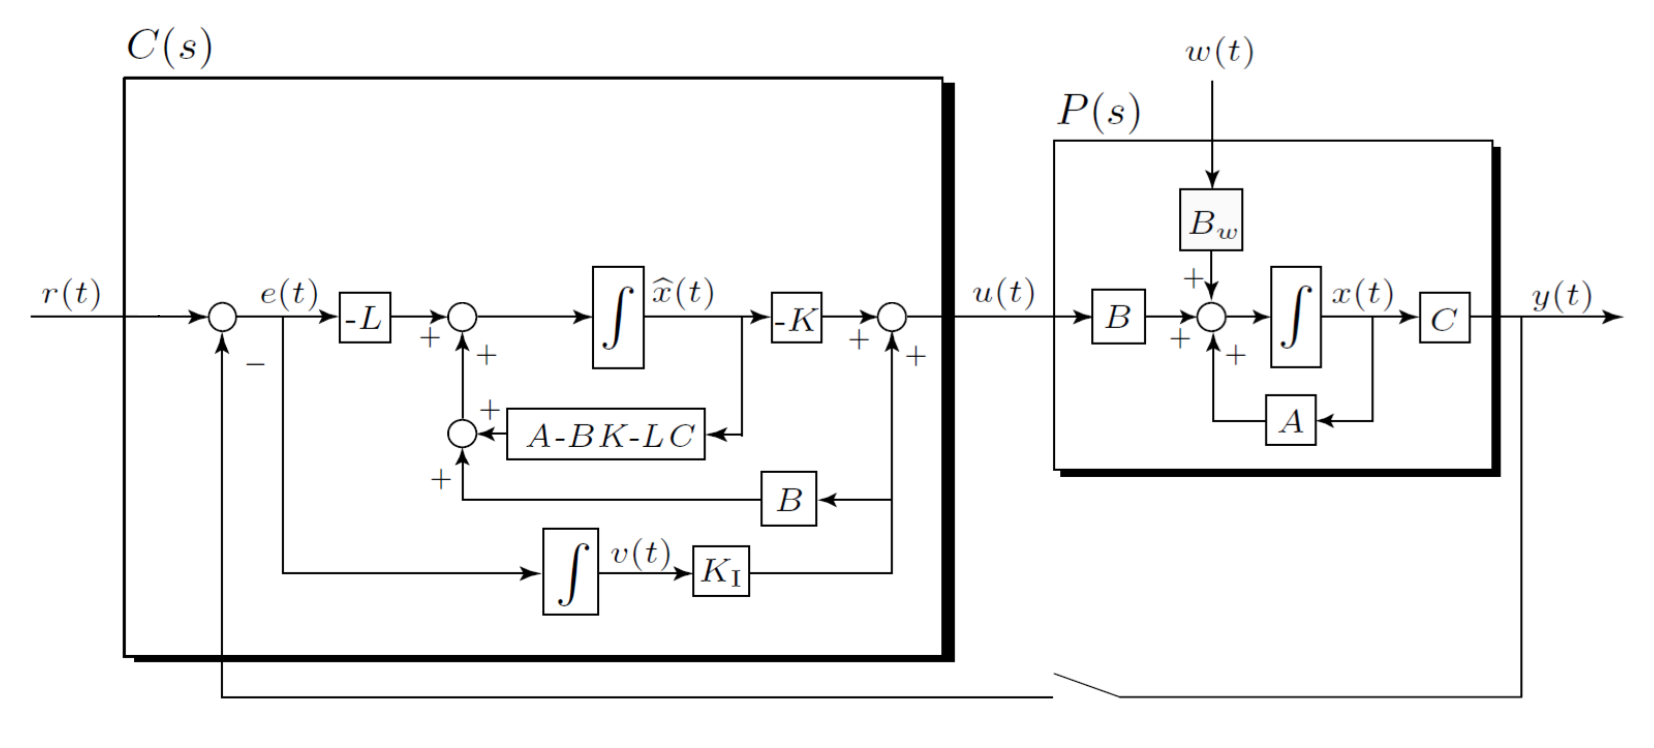
\includegraphics[width=\columnwidth]{lqgi}
\caption{Structure of LQGI controller.}
\label{fig:lqgi}.
\end{figure}
\newpage

\newpage
\pagebreak
\subsection{LTR}
With the methods we have learned so far, we have no guarantee about robustness. The goal of the LTR method is to improve the robustness of the system, in particular if an observer is introduced. 
\subsubsection{Definition}
The main idea is to design a LQR or an observer such that the system is enough \textit{good} and in a second step, design a LQG with tuning parameter, to improve the robustness. This can be seen in Figure \ref{fig:LTR}


\begin{figure}[h]
\centering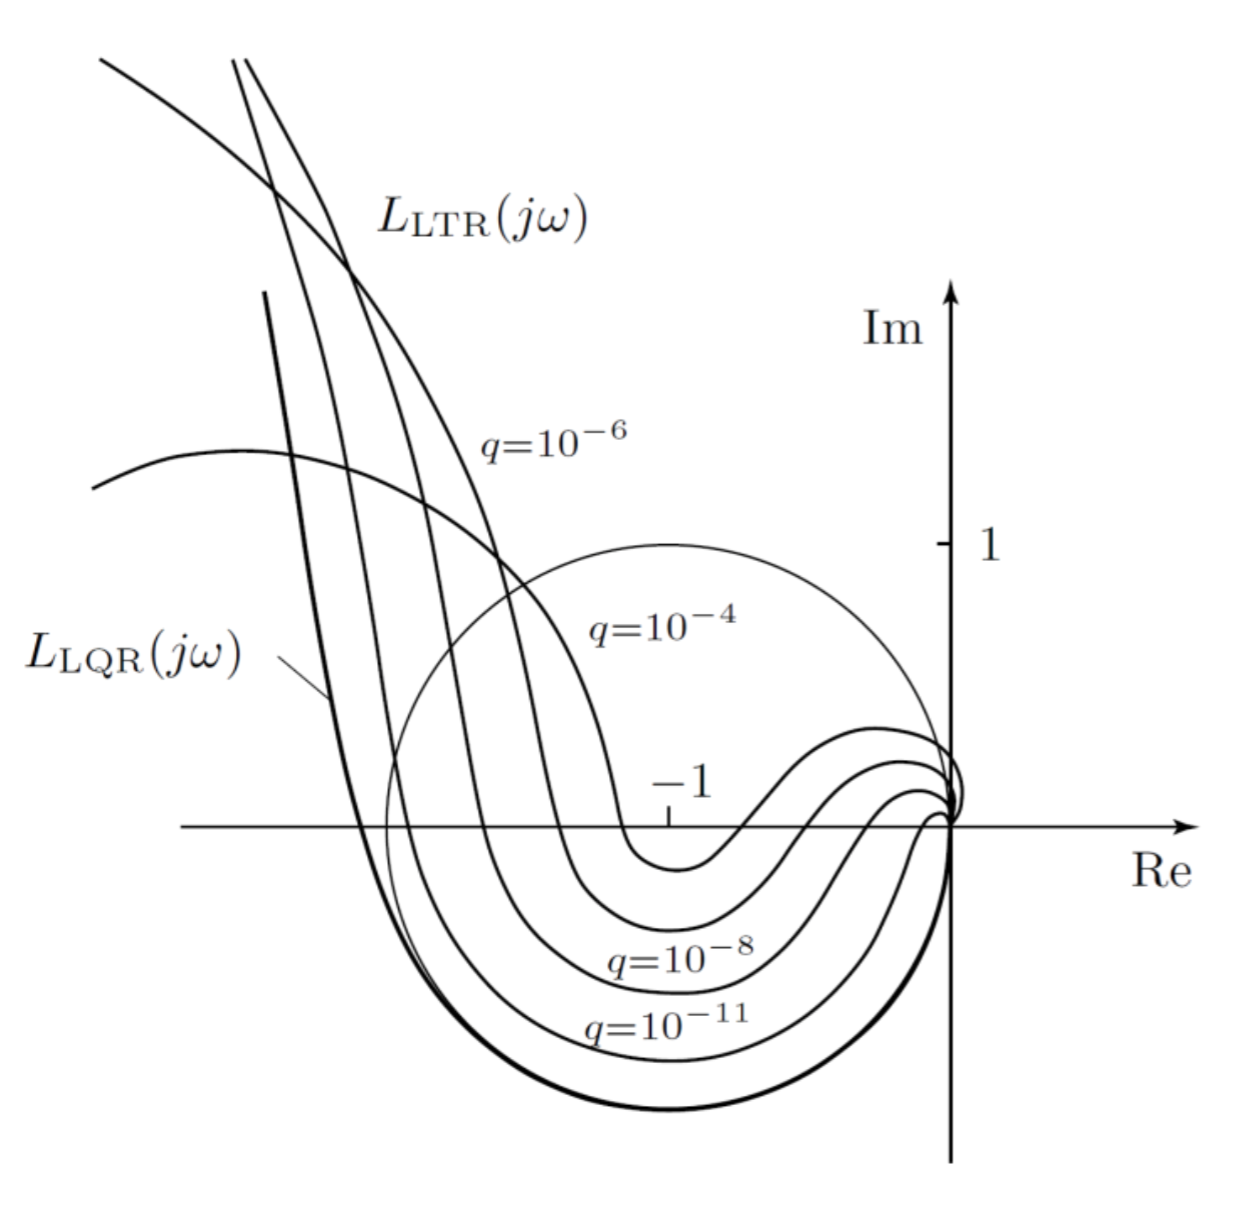
\includegraphics[width=0.5\columnwidth]{LTR}
\caption{LTR.}
\label{fig:LTR}
\end{figure}

\subsubsection{$\beta$ method}
In order to improve the robustness, the $\beta$ method is often chosen:
\subsubsection*{Kochrezept}
\begin{enumerate}[(I)]
\item LQR: Compute $K$ with
\begin{equation}
\frac{1}{r\cdot\beta}\cdot\Phi\cdot B\cdot B^\intercal\cdot \Phi-\Phi\cdot A-A^\intercal\cdot \Phi-Q=0,
\end{equation}
\begin{equation}
K=\frac{1}{r}\cdot B^\intercal\cdot \Phi.
\end{equation}
Matlab: \texttt{Phi = care(A,B,Q,beta*r*eye(nu))}, \texttt{K = 1/r*B'*Phi}.

\item LQG: Compute $L$ with
\begin{equation}
\frac{1}{q\cdot\beta}\cdot \Psi\cdot C^\intercal\cdot C\cdot \Psi-\Psi\cdot A^\intercal-A\cdot\Psi-\bar B\cdot \bar B^\intercal=0,
\end{equation}
\begin{equation}
L^\intercal=\frac{1}{q}\cdot C\cdot\Psi.
\end{equation}
Matlab: \texttt{Psi = care(A',C',B\_bar*B\_bar',beta*q*eye(ny))}, \texttt{L = (1/q*C*Psi)'}.
\end{enumerate}

\begin{bmk}
In order to compute $K$ and $L$ the command \texttt{lqr} was used so far. Since $\beta$ appears only in the Riccati equations for $\Phi$ and $\Psi$, one should first solve the Riccati equation with the command \texttt{care} and then just in a second step compute $K$ and $L$.
\end{bmk}


\subsubsection{LQG/LQR for $m\geq p$}
\begin{enumerate}
\item Modelization of the plant, linearization and normalization;
\item Definition of the specifications in frequency domain;
\item Design of the observer:
\begin{enumerate}
\item \texttt{Psi = care(A',C',B\_bar*B\_bar',beta*q*eye(ny))};
\item \texttt{L = (1/q*C*Psi)'};
\item Find \texttt{B\_bar*B\_bar'}$\in\mathbb{R}^{n\times n}$, $q>0$, and $\beta\leq 1$, s.t. the specifications are fulfilled.
\item Compute $L_\text{obs}$ with
\begin{equation}
L_\text{obs}(s)=C\cdot (s\cdot \mathbb{I}-A)^{-1}\cdot L;
\end{equation}
\end{enumerate}
\item Design of the  ``state feedback regulator'':
\begin{enumerate}
\item \texttt{K = lqr(A,B,C'*Q\_y*C,rho*R\_u)};
\item Find \texttt{Q\_y}$\in\mathbb{R}^{p\times p}$ and \texttt{R\_u}$\in\mathbb{R}^{m\times m}$ (often \texttt{Q\_y = eye(ny)} and \texttt{R\_u = eye(nu)});
\item Choose \texttt{rho} smaller until all the spezifications are fulfilled;
\item Loop gain:
\begin{equation}
L_\text{LTR}(s)=C\cdot (s\cdot \mathbb{I}-A)^{-1}\cdot B\cdot K\cdot(s\cdot\mathbb{I}-(A-B\cdot K-L\cdot C))^{-1}\cdot L;
\end{equation}
\end{enumerate}
\item Implement the controller.
\end{enumerate}


\subsubsection{LQG/LQR for $p\geq m$}
\begin{enumerate}
\item Modelization of the plant, linearization and normalization;
\item Definition of the specifications in frequency domain;
\item Design the LQR:
\begin{enumerate}
\item \texttt{Phi = care(A,B,Q,beta*q*eye(nu))};
\item \texttt{K = 1/r*B'*Phi};
\item Find \texttt{Q}$\in\mathbb{R}^{n\times n}$, $r>0$, and $\beta\leq 1$, s.t. the specifications are fulfilled;
\item Compute $L_\text{obs}$ with
\begin{equation}
L_\text{LQR}(s)=K\cdot (s\cdot \mathbb{I}-A)^{-1}\cdot B;
\end{equation}
\end{enumerate}
\item Design the LTR ``state feedback regulator'' :
\begin{enumerate}
\item \texttt{L = lqr(A',C',B*Q\_u*B',mu*R\_y)'};
\item Find \texttt{Q\_u}$\in\mathbb{R}^{m\times m}$ and \texttt{R\_y}$\in\mathbb{R}^{p\times p}$ (often \texttt{Q\_u = eye(nu)} and \texttt{R\_y = eye(ny)});
\item Choose \texttt{mu} smaller until all the specifications are fulfilled;
\item Loop gain:
\begin{equation}
L_\text{LTR}(s)=C\cdot (s\cdot \mathbb{1}-A)^{-1}\cdot B\cdot K\cdot(s\cdot\mathbb{1}-(A-B\cdot K-L\cdot C))^{-1}\cdot L;
\end{equation}
\end{enumerate}
\item Implement the controller.
\end{enumerate}

\newpage

\appendix
\section{Linear Algebra}
\subsection{Matrix-Inversion}\label{matrixinversion}
\begin{equation*}
A^{-1}=\frac{1}{\det(A)}\cdot\text{adj}(A),\qquad
\{\text{adj}(A)\}_{ij}=(-1)^{i+j}\cdot \det(A_{ij})
\end{equation*}
Special Cases:
\begin{itemize}
\item $n=2$:
\begin{equation*}
A=\begin{bmatrix} a & b \\ c & d \end{bmatrix} \quad \Rightarrow \quad 
A^{-1}=\frac{1}{a\cdot d-b\cdot c}\cdot\begin{bmatrix} d & -b \\ -c & a\end{bmatrix}
\end{equation*}
\item $n=3$:
\begin{equation*}
 A=
\begin {bmatrix}
	a & b & c \\
	d & e & f \\
	g & h & i
\end {bmatrix}\quad \Rightarrow \quad 
A^{-1}= \frac{1}{\det(A)}
\begin{bmatrix}
	e\cdot i-f\cdot h & c\cdot h-b\cdot i & b\cdot f-c\cdot e \\
	f\cdot g-d\cdot i & a\cdot i-c\cdot g & c\cdot d-a\cdot f \\
	d\cdot h-e\cdot g & b\cdot g-a\cdot h & a\cdot e-b\cdot d
\end{bmatrix}
\end{equation*}
\item $(a+b)^3=a^3+3a^2b+3ab^2+b^3$
\end{itemize}

\subsection{Differentiation with Matrices}
\[\dd{}{x} A\cdot x = A^T \]
\[ \dd{}{x} x^T \cdot A \cdot x = (A^T + A)\cdot x\]
\subsection{Matrix Inversion Lemma}\label{minvlemma}
\[[M+ v\cdot v^T]^{-1} = M^{-1} - \frac{1}{1+v^T\cdot M^{-1}\cdot v}\cdot M^{-1}\cdot v \cdot v^T \cdot M^{-1}\]

\newpage
\section{Rules}
\subsection{Trigo}
\begin{center}
\begin{tabular}{lrrrrrrr}
\toprule
\vspace{0.1cm}$\alpha [^\circ]$ & 0 & 30 & 45 & 60 & 90 & 120 & 180 \\ 
$\alpha [\text{rad}]$ & 0 & $\frac{\pi}{6}$ & $\frac{\pi}{4}$ & $\frac{\pi}{3}$ & $\frac{\pi}{2}$ & $\frac{2\pi}{3}$ & $\pi$ \\
\midrule
\vspace{0.1cm}$\sin(\alpha)$ & $0$ & $\frac{1}{2}$ & $\frac{\sqrt{2}}{2}$ & $\frac{\sqrt{3}}{2}$ & $1$ & $\frac{\sqrt{3}}{2}$ & $0$ \\
\vspace{0.1cm}$\cos(\alpha)$ & $1$ & $\frac{\sqrt{3}}{3}$ & $\frac{\sqrt{2}}{2}$ & $\frac{1}{2}$ & $0$ & $-\frac{1}{2}$ & $-1$ \\
\vspace{0.1cm}$\tan(\alpha)$ & $0$ & $\frac{\sqrt{3}}{3}$ & $1$ & $\sqrt{3}$ & $\pm \infty$ & $-\sqrt{3}$ & $0$ \\
$\cot(\alpha)$ & $\pm \infty$ & $\sqrt{3}$ & $1$ & $\frac{\sqrt{3}}{2}$ & $0$ & $-\frac{\sqrt{3}}{2}$ & $\pm \infty$ \\
\bottomrule
\end{tabular}
\end{center}
\subsection{Euler-Forms}
\[ e^{ix}= \cos(x) + i \cdot \sin(x)\]
\[ a+i\cdot b = |a + i \cdot b|\cdot e^{i\cdot\angle(a+i\cdot b)}\]
\[\sin(x)=\frac{1}{2i}(e^{ix}-e^{-ix})\]
\[\cos(x)=\frac{1}{2}(e^{ix}+e^{-ix})\]
\subsection{Derivatives}
\[(\log_a |x|)'=(\log_a e)\frac{1}{x}=\frac{1}{x\ln a}\]		% Formeln und Tafeln, S.37
\[(a^{cx})'=(c\ln a)a^{cx}\]
\[(\tan x)'=\frac{1}{\cos^2 x}=1+\tan^2 x\]
\[(\arcsin x)'=\frac{1}{\sqrt{1-x^2}}\]
\[(\arccos x)'=-\frac{1}{\sqrt{1-x^2}}\]
\[(\arctan x)'=\frac{1}{1+x^2}\]
\subsection{Logarithms}
 \[ \ln |y|\cdot C = \ln |y^C|\]
 \[ - \ln |r| = \ln|r^{-1}|\]
 \[ \ln(1) = \log(1) = 0\]
  \subsection{Magnitude and Phase}\label{betragphase}
 In the Bode diagram are magnitude and phase separate from each other. Magnitude and phase for complex fractions are:
  \[ \Big\vert \frac{a + i \cdot b}{c + i \cdot d}\Big\vert = \sqrt{\frac{a^2 + b^2}{c^2 + d^2}}\]
  \[ \angle \left( \frac{a + i \cdot b}{c + i \cdot d}\right) = \arg \left\{ \frac{a + i \cdot b}{c + i \cdot d}\right\}= \arctan \left( \frac{bc - ad}{ac + bd}\right)\]
  \[ \arg \left\{ a + i \cdot b\right\} = \arctan \left( \frac{b}{a}\right)\]
  \[ \arg \left\{ (a + i \cdot b)^c\right\} = c \cdot \arg \left\{ a + i \cdot b\right\}\]
  \[ \arg \left\{ \frac{c}{(a + i \cdot b)}\right\} = \arg \left\{ c\right\} - \arg \left\{ a + i \cdot b\right\}\]
  \subsection{dB-Skala}
  Typically the unit for the magnitude is dB:
  \[ |\Sigma(j \omega)|_{\textnormal{dB}}=20 \cdot \textnormal{log}_{10} |\Sigma (j \omega)|\]
  \[ |\Sigma (j \omega)| = 10^{\frac{|\Sigma(j \omega)|_{\textnormal{dB}}}{20}}\]
  \[ \frac{1}{X}\Big\vert_{\textnormal{dB}}= -X|_{\textnormal{dB}}\]
  \[ (X\cdot Y)|_{\textnormal{dB}} = X|_{\textnormal{dB}} + Y|_{\textnormal{dB}}\]
  \begin{center}
  \begin{tabular}[width=\columnwidth]{l|rrrrrrrrrr}
  \toprule
  Value& $0.001$&$0.01$ & $0.1$ & $0.5$ & $\frac{1}{\sqrt{2}}$ & $1$ & $\sqrt{2}$ & $2$ & $10$ & $100$ \\
  dB & $-60$ & $-40$ & $-20$ & $\approx -6$ & $\approx -3$ & $0$ &$\approx 3$ & $\approx 6$ & $20$ & $40$\\
  \bottomrule
  \end{tabular}
  \end{center}

\newpage
\section{MATLAB}
\subsection{General Commands}
\begin{center}\begin{tabular}{ll}
\toprule
Command & Description \\
\midrule
\texttt{A(i,j)} & Element of \texttt{A} in position \texttt{i} (row) and \texttt{j} (column) \\
\texttt{abs(X)} & Magnitude of all elements of \texttt{X} \\
\texttt{angle(X)} & Phase of all elements of \texttt{X} \\
\texttt{X'} & Complex conjugate and transpose of \texttt{X} \\
\texttt{X.'} & Transpose, not complex conjugate of \texttt{X} \\
\texttt{conj(X)} & Complex conjugate of all elements of \texttt{X}\\
\texttt{real(X)} & Realteil von allen Eintr\"age von \texttt{X}\\
\texttt{imag(X)} & Imaginary part of all elements of \texttt{X}\\
\texttt{eig(A)} & Eigenvalues of \texttt{A} \\ 
\texttt{[V,D]=eig(A)} & Eigenvalues \texttt{D} (diagonal elements), eigenvectors \texttt{V} (column vectors) \\
\texttt{s=svd(A)} & singular values of \texttt{A} \\
\texttt{[U,Sigma,V]=svd(A)} & Singular Values Decomposition of \texttt{A} \\
\texttt{rank(A)} & Rank of \texttt{A} \\
\texttt{det(A)} & Determinant of \texttt{A} \\
\texttt{inv(A)} & Inverse of \texttt{A} \\
\texttt{diag([a1,\ldots,an])} & Diagonalmatrix with \texttt{a1,\ldots,an} as diagonal elements\\
\texttt{zeros(x,y)} & Zero matrix of dimension \texttt{x}$\times$\texttt{y} \\
\texttt{zeros(x)} & Zero matrix of dimension \texttt{x}$\times$\texttt{x} \\
\texttt{eye(x,y)} & Identity matrix of dimension \texttt{x}$\times$\texttt{y} \\
\texttt{eye(x)} & Identity matrix of dimension \texttt{x}$\times$\texttt{x} \\
\texttt{ones(x,y)} & One-Matrix (all elements = 1) of dimension \texttt{x}$\times$\texttt{y} \\
\texttt{ones(x)} & One-Matrix (all elements = 1) of dimension \texttt{x}$\times$\texttt{x} \\
\texttt{max(A)} & Largest element in vector \texttt{A} (\texttt{A} Matrix: Max in column vectors) \\
\texttt{min(A)} & Smallest element in vector \texttt{A} (\texttt{A} Matrix: Max in column vectors) \\
\texttt{sum(A)} & Sum of elements of \texttt{A} (\texttt{A} Matrix: Sum row pro row) \\
\texttt{dim=size(A)} & Dimension of \texttt{A} (\texttt{size=[\#rows \#columns]})\\
\texttt{dim=size(A,a)} & \texttt{a=1}: \texttt{dim=\#rows}, \texttt{a=2}: \texttt{dim=\#columns}, sonst \texttt{dim=1}\\
\texttt{t=a:i:b} & \texttt{t=[a,a+i,a+2i,\ldots,b-i,b]} (row vector) \\
\texttt{y=linspace(a,b)} & row vector with 100 ``linear-spaced'' points in range \texttt{[a,b]} \\
\texttt{y=linspace(a,b,n)} & row vector with \texttt{n} ``linear-spaced'' points in range \texttt{[a,b]} \\
\texttt{y=logspace(a,b)} & row vector with 50 ``logarithmically-spaced'' points in range \texttt{[10\^{}a,10\^{}b]} \\
\texttt{y=logspace(a,b,n)} & row vectors with \texttt{n} ``logarithmically-spaced'' points in range \texttt{[10\^{}a,10\^{}b]} \\
\texttt{I=find(A)} & \texttt{I}: Index of non zero elements of \texttt{A} \\
\texttt{disp(A)} & Print on screen of \texttt{A} (String: \texttt{'name'}) \\
\bottomrule
\end{tabular}
\end{center}


\newpage
\subsection{Control Systems Commands}
\begin{center}
\begin{tabular}{ll}
\toprule
Befehl & Beschreibung \\
\midrule
\texttt{sys=ss(A,B,C,D)} & State-Space M. with \texttt{A,B,C,D} in time domain \\
\texttt{sys=ss(A,B,C,D,Ts)} & State-Space M. with \texttt{A,B,C,D} and sampling \texttt{Ts} (discrete-time) \\
\texttt{sys=zpk(Z,P,K)} & State-Space M. with zeros \texttt{Z}, poles \texttt{P} and gain \texttt{K} \\
\texttt{sys=zpk(Z,P,K,Ts)} & State-Space M. with zeros \texttt{Z}, poles \texttt{P}, gain \texttt{K} and sampling \texttt{Ts} \\
\texttt{sys=tf([bm \ldots b0],[an \ldots a0])} & Transfer function with  \texttt{bn} in numerator and \texttt{an} in denom. \\
\texttt{P=tf(sys)} & \ Transfer function of \texttt{sys} \\
\texttt{P.iodelay=\dots} & Insers to \texttt{P} delay.\\
\texttt{pole(sys)} & Poles of System \\
\texttt{zero(sys)} &  Zeros og System \\
\texttt{[z,p,k]=zpkdata(sys)} & \texttt{z}: Zeros, \texttt{p}: Poles, \texttt{k}: static gain\\
\texttt{ctrb(sys)} or \texttt{ctrb(A,b)} & Controllability Matrix \\
\texttt{obsv(sys)} or \texttt{obsv(A,c)} & Observability Matrix \\
\texttt{series(sys1,sys2)} & series of \texttt{sys1} and \texttt{sys2} \\
\texttt{feedback(sys1,sys2)} & \texttt{sys1} with  \texttt{sys2} as (negative) Feedback \\
\texttt{[Gm,Pm,Wgm,Wpm]=margin(sys)} &
\texttt{Gm}: gain margin, \texttt{Pm}: phase margin, \texttt{Wpm}: crossover freq. \\
\texttt{[y,t]=step(sys,Tend)} & \texttt{y}: step response von \texttt{sys} until \texttt{T}, \texttt{t}: time\\
\texttt{[y,t]=impulse(sys,Tend)} & \texttt{y}: impulse response of \texttt{sys} until \texttt{Tend}, \texttt{t}: time\\
\texttt{y=lsim(sys,u,t)} & Simulation of \texttt{sys} with input \texttt{u} for the time\texttt{t} \\
\texttt{sim('Simulink model',Tend)} & Simulation of \texttt{Simulink Model'} until \texttt{Tend} \\
\texttt{p0=dcgain(sys)} & static gain ($P(0)$) \\
\texttt{K=lqr(A,B,Q,R)} & Gain Matrix \texttt{K} (solution of the LQR-Problem) \\
\texttt{[X,L,K]=care(A,B,Q)} & \texttt{X}: solution of the Riccati equation, \texttt{G}: Gain matrix \\
\texttt{Paug=augw(G,W1,W3,W2)} & Space State M. for $\mathcal{H}_\infty$ \\
\texttt{[K,Cl,gamma]=hinfsyn(Paug)} & $\mathcal{H}_\infty$ : \texttt{K}: Controller \\
\texttt{fr=evalfr(sys,f)} & \texttt{sys} evaluated in \texttt{f} $(s=f)$ \\
\texttt{sysd=c2d(sys,Ts,method)} & Discretization of \texttt{sys} with \texttt{method} with Sampling Time \texttt{Ts} \\
\bottomrule
\end{tabular}\end{center}

\newpage
\subsection{Plot and Diagrams}
\begin{center}\begin{tabular}{ll}
\toprule
Befehl & Beschreibung \\
\midrule
\texttt{nyquist(sys)} & Nyquist diagram of the system \texttt{sys} \\
\texttt{nyquist(sys,\{a,b\})} & Nyquis diagramm in interval \texttt{[a,b]} of the system \texttt{sys}\\
\texttt{bode(sys)} & Bode diagram of the system \texttt{sys}\\
\texttt{bode(sys,\{a,b\})} & Bode diagram in intervall \texttt{[a,b]} of the system \texttt{sys}\\
\texttt{bodemag(sys)} & Bode diagram (just magnitude) of the system \texttt{sys}\\
\texttt{bodemag(sys,\{a,b\})} & Bode diagram (just magnitude) in interval \texttt{[a,b]} of the system.  \texttt{sys}\\
\texttt{rlocus(sys)} & Root Locus diagram\\
\texttt{impulse(sys)} & Impulse Response of the system \texttt{sys}\\
\texttt{step(sys)} & Step response of the system \texttt{sys}\\
\texttt{pzmap(sys)} & Poles and zeros mapping of the  system \texttt{sys} \\
\texttt{svd(sys)} & Singular values dynamics of the dystem \texttt{sys} \\
\texttt{plot(X,Y)} & Plot of \texttt{Y} as function of \texttt{X} \\
\texttt{plot(X,Y,\ldots,Xn,Yn)} & Plot of \texttt{Yn} as function of \texttt{Xn} (for all \texttt{n})\\
\texttt{stem(X,Y)} & Discrete plot of \texttt{Y} as function of \texttt{X} \\
\texttt{stem(X,Y,\ldots,Xn,Yn)} & Discrete plot of \texttt{Yn} as function of \texttt{Xn} (for all \texttt{n}) \\
\texttt{xlabel('name')} & Name of the \texttt{x}-Axis \\
\texttt{ylabel('name')} & Name of the \texttt{y}-Axis \\
\texttt{title('name')} & Title of the plot\\
\texttt{xlim([a b])} & Range for the \texttt{x}-Axis (Plot between \texttt{a} and \texttt{b}) \\
\texttt{ylim([a b])} & Range for the \texttt{y}-Axis (Plot between \texttt{a} and \texttt{b}) \\
\texttt{grid on} & Grid \\
\texttt{title('name')} & Title of the plot \\
\texttt{legend('name1',\ldots,'name')} & Legend \\
\texttt{subplot(m,n,p)} & Grid \texttt{m$\times$n}, Plot in Position \texttt{p} \\
\texttt{semilogx(X,Y)} & Logarithmitic Plot with \texttt{y}-Axis linear \\
\bottomrule
\end{tabular}\end{center}








\end{document}




